\documentclass[12pt, fullpage]{article}
\usepackage{uhthesis2019}
\usepackage{graphicx}
\usepackage{geometry}
\usepackage{amsmath}
\usepackage{adjustbox}
\usepackage{booktabs}
\usepackage{placeins}
\usepackage{subcaption}
\usepackage{floatrow}
\newcommand{\GG}[1]{}
\usepackage{multicol}
\usepackage{multirow}
\usepackage{natbib}
\usepackage{siunitx}
\newcolumntype{d}{S[input-symbols = ()]}
\usepackage{lscape}
\usepackage{lscape}
\newcommand{\ts}{\textsuperscript}
\usepackage{threeparttablex}
\floatsetup[table]{capposition=top}
\floatsetup[figure]{capposition=top}
\usepackage{caption}
\captionsetup[table]{name=TABLE}
\renewcommand{\thetable}{\Roman{table}}
\captionsetup[table]{skip=3pt}
\usepackage{makecell}
\usepackage{longtable}
\usepackage{tabularx}
\renewcommand{\tabularxcolumn}{m}
\usepackage{threeparttable}
\newcommand{\note}[1]{\flushleft\footnotesize{#1}}

\renewcommand{\thetable}{\arabic{table}}  
\renewcommand{\thefigure}{\arabic{figure}}
\newcommand{\source}[1]{\caption*{Source: {#1}} }
% *****************************************************************
% Estout LaTeX wrapper
% *****************************************************************

%%Original code developed by Jörg Weber: see
%% https://www.jwe.cc/2012/03/stata-latex-tables-estout/
%% andwho
%% https://www.jwe.cc/blog/


\let\estinput=\input % define a new input command so that we can still flatten the document

\newcommand{\estwide}[3]{
        \vspace{.75ex}{
            \begin{tabular*}{\textwidth}{@{\extracolsep{\fill}}l*{#2}{#3}}
            \toprule
            \estinput{#1}
            \bottomrule
            \addlinespace[.75ex]
            \end{tabular*}
            }
        }   


\newcommand{\estauto}[3]{
        \vspace{.75ex}{
            %\textsymbols% Note the added command here
            \begin{tabular}{l*{#2}{#3}}
            \toprule
            \estinput{#1}
            \bottomrule
            \addlinespace[.75ex]
            \end{tabular}
            }
        }

% Allow line breaks with \ in specialcells
\newcommand{\specialcell}[2][c]{%
    \begin{tabular}[#1]{@{}c@{}}#2\end{tabular}
}

\newcommand{\sym}[1]{\rlap{#1}}% Thanks David Carlisle


%%%%%%%%%%% End of wrapper %%%%%%%%%%%%%%%%%%%%%
    
%%%%%%%%%%% TiKz %%%%%%%%%%%%%%%%%%%%%
\usepackage{tikz}
\usetikzlibrary{shapes.geometric, arrows}

\tikzstyle{startstop} = [rectangle, rounded corners, minimum width=3cm, minimum height=1cm,text centered, draw=black, fill=red!30]

\tikzstyle{io} = [trapezium, trapezium left angle=70, trapezium right angle=110, minimum width=3cm, minimum height=1cm, text centered, text width =5cm, draw=black, fill=blue!30]

\tikzstyle{process} = [rectangle, minimum width=3cm, minimum height=1cm, text centered, text width =5cm, draw=black, fill=orange!30]

\tikzstyle{decision} = [diamond, minimum width=3cm, minimum height=1cm, text centered, draw=black, fill=green!30]

\tikzstyle{arrow} = [thick,->,>=stealth]

\begin{document}

\pagenumbering{roman}
\title{Essays on Applied Microeconomics}
\author{Hussain Hadah}
\degree{Doctor of Philosophy}{dissertation}
\department{Economics}
\college{College of Liberal Arts and Social Sciences}
    \chair{Chinhui Juhn}
    \cochair{Vikram Maheshri}
    \firstreader{Willa Friedman}
    \secondreader{Yona Rubinstein}
    \threereadersfalse
    \fourreadersfalse
    \fivereadersfalse
    \submitdate{May 2023}
    \figurelisttrue
    \tablelisttrue
\makecoverpages

\newpage
\pagebreak

\noindent\begin{tabular}{ll}
\makebox[2.5in]{\hrulefill} & \makebox[2.5in]{\hrulefill}\\
Chinhui Juhn & Vikram Maheshri\\[8ex]% adds space between the two sets of signatures
\makebox[2.5in]{\hrulefill} & \makebox[2.5in]{\hrulefill}\\
Willa Friedman & Yona Rubinstein\\ [8ex]
\end{tabular}


\begin{dedication}
\textit{Four score and seven years ago our fathers brought forth on this continent, a new nation, conceived in Liberty, and dedicated to the proposition that all men are created equal.}

\textit{Now we are engaged in a great civil war, testing whether that nation, or any nation so conceived and so dedicated, can long endure. We are met on a great battle-field of that war. We have come to dedicate a portion of that field, as a final resting place for those who here gave their lives that that nation might live. It is altogether fitting and proper that we should do this.}

\textit{But, in a larger sense, we can not dedicate -- we can not consecrate -- we can not hallow -- this ground. The brave men, living and dead, who struggled here, have consecrated it, far above our poor power to add or detract. The world will little note, nor long remember what we say here, but it can never forget what they did here. It is for us the living, rather, to be dedicated here to the unfinished work which they who fought here have thus far so nobly advanced. It is rather for us to be here dedicated to the great task remaining before us -- that from these honored dead we take increased devotion to that cause for which they gave the last full measure of devotion -- that we here highly resolve that these dead shall not have died in vain -- that this nation, under God, shall have a new birth of freedom -- and that government of the people, by the people, for the people, shall not perish from the earth.}

\begin{flushright}
Abraham Lincoln \\
November 19, 1863
\end{flushright}
\end{dedication}

\begin{acknowledgements}
\singlespacing{
    Lorem ipsum dolor sit amet, consectetur adipiscing elit, sed do eiusmod tempor incididunt ut labore et dolore magna aliqua. Mi proin sed libero enim sed faucibus turpis in eu. Feugiat vivamus at augue eget arcu dictum. Sit amet dictum sit amet justo donec. Vitae nunc sed velit dignissim sodales ut eu sem integer. Aliquam etiam erat velit scelerisque in dictum non consectetur a. Et sollicitudin ac orci phasellus egestas tellus. Maecenas pharetra convallis posuere morbi leo urna molestie. Erat nam at lectus urna duis convallis. Turpis egestas sed tempus urna.
}
\end{acknowledgements}

\begin{abstract}
    \doublespacing
    Lorem ipsum dolor sit amet, consectetur adipiscing elit, sed do eiusmod tempor incididunt ut labore et dolore magna aliqua. Mi proin sed libero enim sed faucibus turpis in eu. Feugiat vivamus at augue eget arcu dictum. Sit amet dictum sit amet justo donec. Vitae nunc sed velit dignissim sodales ut eu sem integer. Aliquam etiam erat velit scelerisque in dictum non consectetur a. Et sollicitudin ac orci phasellus egestas tellus. Maecenas pharetra convallis posuere morbi leo urna molestie. Erat nam at lectus urna duis convallis. Turpis egestas sed tempus urna.
    \cleardoublepage
    \singlespacing
\end{abstract}

%Optional Copyright Page
\copyrighttrue
\makecontentspages

\pagenumbering{arabic}

\section[\bf \uppercase{The Impact of Hispanic Last Names and Identity on Labor Market Outcomes}]{The Impact of Hispanic Last Names and Identity on Labor Market Outcomes}

\subsection{Introduction}\label{sec:intro}

There is a plethora of evidence of ethnic and racial discrimination in the labor market \citep{bayer2018divergent, charles2008prejudice, card1992school, fryer2004causes, rubinstein2014pride, bertrand2004emily, juhn1991accounting}. Hispanics constitute a large and growing portion of the population in the United States. As the number of Hispanics keeps increasing in the labor force, identifying whether they face ethnic discrimination grows in importance. Consequently, questions on assimilation and mobility grow in importance \citep{chettyUnitedStatesStill2014, chettyEffectsExposureBetter2016,chettyFadingAmericanDream2017,abramitzkyImmigrantsAssimilateMore2020a, abramitzkyNationImmigrantsAssimilation2014,abramitzkyCulturalAssimilationAge2016,chettyWhereLandOpportunity2014}, how identity could shift public opinions toward trade \citep{grossmanIdentityPoliticsTrade2021}, and how racial and gender attitudes affect the racial and gender earnings gaps \citep{charlesPrejudiceWagesEmpirical2008,charlesEffectsSexismAmerican2018}. Thus, it is important to understand whether a person's ethnicity affects their labor market outcomes.

In this paper, I answer the following questions. Does having a Hispanic last name affect labor market outcomes? What is the effect of identifying as Hispanic on earnings? Moreover, I aim to show that comparing Hispanic Whites to non-Hispanic Whites might create an artificially higher earnings gap since the two groups differ on many observable characteristics. Others have attempted to compare how native-born White Hispanics fare to non-Hispanic Whites and foreign-born Hispanics. In \citet{antman2020ethnic,antmanEthnicAttritionObserved2016,antmanEthnicAttritionObserved2016a,antmanEthnicAttritionAssimilation2020}, the authors compare the health and educational outcomes of Hispanic Whites to non-Hispanic Whites and native-born Hispanics to foreign-born Hispanics. They find gaps in education and health between Hispanics and Whites. They also find that native-born Hispanics are more likely than their foreign-born counterparts to report poor health. \citet{davilaChangesRelativeEarnings2008}, the authors documents many gaps in labor market outcomes between Hispanics and Whites. They attribute a big part of this gap to differences in education, experience, immigration status, and regional differences. 

The US population is growing in diversity. The proportion of non-Whites has increased by more than 10 percentage points from 1995 to 2019 (see figure \ref{fig:1}), and the number of Hispanics has grown by 9 percentage points over the same period (see figure \ref{fig:2}). Native-born White Hispanic men earn 21\% less than White men \citep{duncan2018identifying}. However, a substantial portion of the earnings gap is due to educational differences between Hispanics and Whites \citep{duncan2006hispanics, duncan2018socioeconomic}. Therefore, understanding discrimination against Hispanics and their children is an important task. Discrimination against Hispanics has a couple of negative consequences. First, if Hispanics face a substantial labor market penalty for their ethnic identity, it could hinder assimilation and integration. Second, a significant labor market penalty contributes to the growing wage gap between Whites and other minority groups. In this paper, I examine the role of having a Hispanic last name and identifying as Hispanic on labor market outcomes. 


Identifying discrimination is difficult because of factors that affect labor market outcomes that are unobservable to economists---like innate ability. Also, I should be able to disentangle skills differentials between Hispanics and non-Hispanic Whites. To causally identify ethnic discrimination against Hispanics and its effects on labor market outcomes, a researcher should compare two identical people that only differ in their last name. Since this approach is unfeasible, researchers took different approaches. \citet{bertrand2004emily} and \citet{fryer2004causes} conducted audit studies to examine the effect of Black sounding names on employment discrimination. This approach, however, has its drawbacks. Audit studies only observe callbacks, not wages. 

I will use a method developed by \citet{rubinstein2014pride} in this research. I will compare children from intermarriages. More precisely, I will reach children of Hispanic fathers and White mothers (henceforth HW) to children of White fathers and Hispanic mothers (henceforth  WH). This approach stems from the fact that marriages are not random. Couples match on several observable characteristics like income, schooling, socio-economic background, etc. \citep{averettBetterWorseRelationship2008, averettEconomicRealityBeauty1996, beckerTheoryMarriagePart1973, beckerTheoryMarriagePart1974, beckerTreatiseFamily1993, browningCollectiveUnitaryModels2006, chiapporiFatterAttractionAnthropometric2012}. Children of HW and WH marriages have more similar observable characteristics than children of homogeneous marriages--- i.e., White fathers-White mothers and Hispanic fathers-Hispanic mothers. Moreover, children from a Hispanic father and White mother household will have a Hispanic last name from their fathers, allowing me to test for ethnic signals on annual log earnings.

Using the Current Population Survey (CPS) from 1994 to 2019 and the 1970-1990 US censuses, I will estimate the effect of having a Hispanic last name on the labor market outcomes. In other words, I will approximate the variation in labor market perception of ethnic signals, in this case having a Hispanic last name, on annual log earnings. I also study the effect of identifying as Hispanic on labor market outcomes. 

To retrieve the effect of having a Hispanic last name, I compare the children of inter-ethnic marriages between Whites and Hispanics. I find that while men born to White father-Hispanic mothers earn less than men born to Hispanic father-White mothers, this gap is entirely explained by educational differences. Thus, I do not find a significant effect of having a Hispanic last name. Finally, I find that men identifying as Hispanic earn significantly less than those who do not, even when I control ancestry and education. 

A long list of economic papers investigated taste-based discrimination, statistical discrimination, and Black-White and gender earnings gaps that date back to the seminal work of \citet{becker2010economics}. \citet{bayer2018divergent} investigated the Black-White wage gap's narrowing and then divergence. \citet{card1992school} argued that the Black-White wage gap narrowed from 1960 to 1980 due to improvement in the quality of Black schools, and \citet{juhn1991accounting} showed that skills play a big part in the Black-White wage gap. Moreover,  \citet{charles2008prejudice} provided evidence that 25\% of the Black-White wage gap is due to prejudice. \citet{black1995discrimination} introduced a search model showing that with a taste for discrimination, minorities earn less than the majority group even when hired by an unprejudiced firm. In comparison, \citet{altonji2001employer} found that firms do not statistically discriminate based on race and ethnicity. Little has been done, however, about discrimination against Hispanics, which offers an opportunity to exploit the observable racial similarities between Hispanics and Whites.

This is not the first attempt to use names as signals for race and ethnicity \citep{fryer2004causes, rubinstein2014pride, bertrand2004emily}. \citet{fryer2004causes} point out that names can be a predictor of a person's race. Specifically, they provide a rising pattern among Blacks having different names than Whites. They did, however, find that having a Black name, after controlling for the home environment at birth, does not affect their labor market outcomes. \citet{rubinstein2014pride} compared the children of mixed marriages between Sephardic and Ashkenazis in Israel. They found that workers with Sephardic last names earn substantially less than those with an Ashkenazi last name. \citet{bertrand2004emily} conducted an audit study by sending employers identical resumes that differ in the ethnic and racial signal of a name (Black sounding name versus a White sounding one). They found that resumes with Black-sounding names received substantially fewer callbacks than their White counterparts. 

The rest of the paper is organized as follows. Section \ref{sec:data} provides an overview of the data and summary statistics of the sample I am using. Section \ref{sec:emp_model} introduces a formal empirical model. I go over the results in section \ref{sec:results}. Finally, I offer a brief conclusion in section \ref{sec:con}.

\subsection{Data}\label{sec:data}

For this paper, I will use two data sets. The Integrated Public Use Microdata Series (IPUMS) Current Population Survey (CPS) Annual Social and Economic (ASEC) \citep{cps2019} and the 1970 to 1990 US censuses \citep{acs2019}. 

I use the CPS' rich data set to study the effect of having a Hispanic last name on a person's labor market outcomes. I take advantage of the fact that the CPS asks for parents' place of birth, ethnicity, and race. The data spans the period between 1994--- the earliest sample to ask about a parent's place of birth--- to 2019. Moreover, since the CPS does not provide data on parents' characteristics, essential to determine the family background, I use the census to construct synthetic parents. The census offers a more significant sample of potential parents. Similar to the CPS, the 1970 to 1990 censuses ask about the person's place of birth and the individual's race and ethnicity. I employ this information to construct "synthetic parents" using a method developed by \citet{rubinstein2014pride}. 

I construct the synthetic parents by linking husbands and wives in the census data to each other. I assume that parents have children between the ages of 25 and 40. I then link these synthetic parents using the year they were surveyed to the year of birth of the "children" in the CPS sample.

\subsection{Children of the four parents' types}
I will use the CPS for my primary analysis of the effect of having a Hispanic last name on earnings. I restrict my sample to Whites, United States-born citizens aged 25 to 40 and born between 1970 to 1990. Taking advantage of data on parents' place of birth, I divide the sample into four groups depending on their parent's ethnicity. Mothers or fathers are Hispanic if they were born in a Spanish-speaking country and Puerto Rico, and White if they were born in the United States.\footnote{The list of Spanish Speaking countries include: Argentina, Bolivia, Chile, Colombia, Costa Rica, Cuba, Dominican Republic, Ecuador, El Salvador, Guatemala, Equatorial Guinea, Honduras, Mexico, Nicaragua, Panama, Paraguay, Peru, Spain, Uruguay, Venezuela.} Therefore, an observation can be the product of four types of parents: 
\begin{enumerate}
\item White father and White mother (hereafter WW) 
\item White father and Hispanic mother (hereafter WH)
\item Hispanic father and White mother (hereafter HW)
\item Hispanic father and Hispanic mother (hereafter HH).
\end{enumerate}
The distribution of the four types of children is presented in figure \ref{fig:dist}. The majority of the sample, 95.14\%, is WW children. The second biggest group is HH, which constitutes 3.36\% of the sample. Inter-ethnic children, WH and HW, make up 1.78\% of the sample with 60,147 observations. Even though WH and HW are only 1.78\% of the sample, I have plenty of observations to carry out an analysis. The summary statistics for the children of the four types of marriages are presented in table \ref{tab:c&p1}. Children of WW marriages (column i) do better on every measure while children of HH parents (column iv) do worse than other children on every measure. 

On the one hand, WW children are more educated, with approximately 14 years of education for men and women. man and woman WW children have an employment rate of 95\%. They have log hourly earnings of 2.557 for men and 2.435 for women. Also, their annual log earnings are 10.529 for men and 10.297 for women.

On the other hand, children of HH marriages have an average of 12.898 and 13.204 years of education for men and women, respectively. HH men and women have an employment rate of 93\%. Their annual log earnings are 10.365 and 10.175 for men and women, respectively. 

Inter-ethnic children, WH and HW, have lower educational attainment and income than WW children, but they are better than HH children. Also, WH and HW are comparable, unlike WW and HH children. These two groups are important to my analysis. Children of HW are going to be the treatment group. HW's children have a Hispanic father, who will carry his Hispanic last name. At the same time, the WH children have White fathers and will take his non-Hispanic, or White, last name. A first glance at the summary statistics of these two groups, table \ref{tab:c&p1} columns (ii) and (iii) can show that they are different from the children of non-intermarriages. 

WH children have an average of 13.366 and 13.741 years of education for men and women. The employment rate for men is 94.5\% and for women 95.0\%. HW man and woman children obtained 13.072 and 13.270 years of schooling. Men's employment rate is 92.7\% and women's 93.1\%.

In panel D of table \ref{tab:c&p1}, I present the rates at which members of each group self-identify as Hispanic \footnote{Hispanic self-identification is observed when an individual notes that they are Hispanic on the CPS questionnaire}. The vast majority of HH children, 97\%, identify as Hispanic. There is considerable attrition in Hispanic identification of inter-ethnic children. Among WH children, 82.1\% of men and 85.0\% of women identified as Hispanic. Among HW children, 87.9\% of men and 85.9\% of women identified as Hispanic. These results align with the findings of a substantial body of literature that noted this attrition among children of immigrants, especially those coming from inter-ethnic marriages \citep{duncan2017complexity, duncan2018identifying, duncan2020new, antman2020ethnic}. Finally, a small portion of WW children, 6\%, identified as Hispanic. These 6\% of WW children are most likely third generation--- or more--- immigrants. For my analysis, I dropped the WW observations identified as Hispanic to compare with non-Hispanic Whites.

In columns (v) and (vi), I calculate the differences in means between HH-WW (column v) and HW-WH (column vi). Overall, HH children do worse than WW children. HH has one less year of education compared to WW, 2.1 percentage points less likely to be employed, HH men earn 16.4\% less than WW men, and HH women make 12.3\% less than WW women. Therefore, these two groups, HH and WW, are different in many observable.

The differentials between WH and HW are not as severe as the ones between HH and WW. HW children are still worse off than WH but are way better than HH. HW men attain 0.294 fewer years of education than WH men. HW women achieve 0.471 fewer years of schooling than WH women. HW children are 1.8-1.9 percentage points less likely to be employed. HW men earn the same annual earnings as WH men, and HW women earn 10.3\% less. These differences show that HW and WH children are different from children of homogeneous marriages and, thus, are more comparable.

Moreover, in table \ref{tab:c&p2}, I present the summary statistics for the four types but limit the sample to those that only identify as Hispanic\footnote{Limiting the sample to those that identify as Hispanic only affects WH, HW, and HH. Members of the WW group are not affected by this restriction.}. The same pattern discussed above between HH--WW and HW--WH persists. The one difference is that those who identify as Hispanic do slightly worse.
 %In columns five and six of table \ref{tab:c1}, I present the gaps between HH and WW children and HW and WH children, respectively. The gap between HH and WW children (column five) shows a consistent story, HH children are worse in education and work more. HH children have more kids. While the gap between HW and WH does not have a clear-cut direction. Even though WH children obtain more years of education and have a higher employment rate, HW and WH men have the same fertility rates. HW women have a higher fertility rate than WH women. WH and HW women have the same employment rate.
 
\subsection{Synthetic parents}

Using the 1970 and 1990 censuses, I constructed a panel of synthetic parents. The sample includes married White men and women. Even though the census asks a person whether they are Hispanic or not, I took advantage of the questions on place of birth to create a proxy for ethnicity. I consider a Hispanic person as White and born in a Spanish-speaking country. Consequently, Whites in the sample are people who are White and native-born. Using the information provided in the census, I can link husbands and wives with each other. I assume that parents have children between the ages of 25 and 45. Therefore, my sample consists of married White men and women that were born in the 1930 to 1965 cohorts\footnote{The construction of "synthetic parents" follows the method used by \citet{rubinstein2014pride}.}.

I show the distribution of the four types of couples in table \ref{tab:mat1}. White husbands and White wives (WW) make up the majority of couples in the sample, 98.18\% (681,206 couples). Hispanic husbands and wives (HH) are the second largest group making up 1.04\% (7,193 couples)of all couples. White husbands and Hispanic wives (WH) couples are 0.40\% (2,750 couples) of the sample while Hispanic husbands and White wives (HW) are 0.39\% (2,710 couples). 

I present the summary statistics of the four types of synthetic parents in table \ref{tab:c&p1}'s parent's panel. WW couples have higher education, 11.9 years for husbands and 11.8 for wives. As a household, WW couples have 25.194 years of schooling. Husbands in HH marriages have 8.5 years of education, while women have 8.2 years of schooling. As a household, HH couples have 17.539 years of education.

WH husbands have 10.3 years of education, while wives have an average of 9.6 years, the lowest of any group. WH household attained a total of 22.308 years of schooling in total. HW husbands and wives obtained 9.7 and 9.8 years of education, respectively. HW household attained a total of 21.473 years of schooling in total.

In columns (v) and (vi) of table \ref{tab:c&p1}, I calculated the differences in means between HH-WW households and HW-WH households. An HH Hispanic husband attained 3.779 fewer years of education than a WW husband. While an HH wife acquired 3.876 fewer years of schooling than a White WW wife. The total educational difference between HH and WW households equals 7.655 years of education. The educational differences between HW and WH are less severe than those between HH and WW. A Hispanic husband in intermarriage attained 1.560 fewer years of schooling than a White husband in intermarriage. A White wife in intermarriage attained 0.726 years of education, more than a Hispanic wife in intermarriage. The difference in total years of education between HW and WH households is 0.835, which is an 89\% decrease from the HH--WW gap. These differences show that couples that intermarry are better and different than those that do not.

%In table \ref{tab:p1} columns five and six, I provide the  HH-WW and HW-WH gaps. WW couples are more educated and earn more than HH couples. Also, WH husbands are more educated and earn more than HW husbands. In comparison, WH wives are more educated than HW wives. Even though White husbands in intermarriages are more educated and earn more than husbands in HW marriages, they are more comparable to each other than the non-intermarriage couples.

\subsection{Empirical Strategy}\label{sec:emp_model}
In this section, I will present two empirical strategies. The first empirical strategy will estimate the effect of having a Hispanic last name on annual log earnings. The second empirical strategy will estimate the effect of identifying as Hispanic on log yearly earnings.

The difference in means between Hispanics and non-Hispanic Whites could result from discrimination. It can also be caused by differences in innate abilities, skills, and parental investments during infancy. To avoid these threats to identification, I compare children of intermarriages, HW and WH. WH and HW children are equally Hispanic physically but provide employers/labor market with different signals.\footnote{WH and HW children are both half White, half Hispanic.} WH children will have a non-Hispanic last name, while HW children will have a Hispanic last name. This is a method developed by \citet{rubinstein2014pride}.

\subsection{Estimating the effect of having a Hispanic last name}

Let $Y_{it}$ be the annual log earnings of person $i$ at time $t$. $WH_{i}$, $HW_{i}$ and $HH_{i}$ are indicator variables for the type of parents person $i$ has. $X_{it}$ is a vector of controls, $\gamma_{t}$ are year fixed effects and $\phi_{it}$ represents the error term. The equation for this strategy is written as follows:
\begin{equation} \label{eq:1a}
Y_{it} = \beta_{1} WH_{i} +\beta_{2} HW_{i} + \beta_{3} HH_{i} + X_{it} \pi + \gamma_{t}+\phi_{it}
\end{equation}

$\beta_{1}, \beta_{2}$ and $\beta_{3}$ are the coefficients of interest in this specification. They estimate the earnings gaps between the three groups and children of White-White parents. The difference between $\beta_{1}$ and $\beta_{2}$ captures the effect of having a Hispanic last name. This comes from the fact that the WH and HW children are similar. On the one hand, WH children will have a White father and carry his White last name. On the other hand, HW children will have a Hispanic father and carry his Hispanic last name. Therefore, \textit{ceteris paribus}, the difference will capture the effect of having a Hispanic last name.

\subsection{Estimating the effect of identifying as Hispanic}

In this section, I will present an estimation strategy that would allow me to capture the effect of identifying as a Hispanic. The empiricism in the section follows the theoretical identity model developed by \citet{akerlof2000economics}. 

Let $Y_{it}$ be the annual log earnings of person $i$ at time $t$. $WH_{i}$, $HW_{i}$ and $WW_{i}$ are indicator variables for the type of parents person $i$ has. $X_{it}$ is a vector of controls, $\gamma_{t}$ are year fixed effects and $\phi_{it}$ represents the error term. The addition to the previous model is the $Hispanic_{i}$ indicator variable. $Hispanic_{i}$ is equal to one if a person identifies as Hispanic and zero otherwise. I interact this term with the $WH_{i}$, $HW_{i}$ and $HH_{i}$.  The regression is presented in the following equation.

\begin{align} \label{eq:iden}
Y_{it} &= \beta_{1} HW_{i} +  \beta_{2} WH_{i} + \beta_{3} HH_{i} +\\
& \beta_{4} WH_{i} \cdot Hispanic_{i} + \beta_{5} HW_{i}\cdot Hispanic_{i} +  \beta_{6} HH_{i} \cdot Hispanic_{i}+ \nonumber \\
&X_{it} \pi + \gamma_{t}+\phi_{it} \nonumber
\end{align}

The coefficients of interest from equation \ref{eq:iden} are $\beta_{4}$, $\beta_{5}$ and $\beta_{6}$. The interaction terms capture the earnings gaps between members of $WH_{i}$, $HW_{i}$, and $WW_{i}$ that identify as Hispanic and White WW children. 

\subsection{Results and Discussion}\label{sec:results}

In this section, I present the results from estimating the two specifications in equations \ref{eq:1a} and \ref{eq:iden}. The results are shown in tables \ref{tab:lastnamereg} and \ref{tab:identreg}. All estimations are done on a sample of White, native-born men between the ages of 25 and 40 employed for full-time full-year (FTFY) and are waged and salaried workers.

I find that the earnings gaps between WH and WW are 8.8\%, 14.1\% between HW and WW, and 16.1\% between HH and WW. Moreover, the difference in earnings between HW and WH children, which captures the effect of having a Hispanic last name, equals a statistically significant 5.3 percentage points. Meaning by comparing inter-ethnic children, a person with a Hispanic last name earns 5.3 percentage points less than someone with a White last name. However, more than half of the earnings gaps could be explained by educational differences between WW children and WH, HW, and HH. When I control for education, the gap between the three groups and WW is cut between 50-64.0\%. Furthermore, the last name effect decreases to a statistically insignificant 1.6 percentage points earnings gap.

I also find a significant earnings gap between those that identify as Hispanic and WW children. The gaps between WH, HW, and HH that identify as Hispanic and WW are, respectively, 13.4\%, 16.4\%, and 10.6\%. The difference between WH and HW that identify as Hispanic---captures the last name effect of those that identify as Hispanic--- is equal to 3 percentage points and is statistically insignificant. Controlling for education explains a big part of the gap. The gaps between WH, HW, and HH that identify as Hispanic and WW after controlling for education are 6.4\%, 10.8\%, and 6.2\%. The WH--WW and HH--WW gaps for those identifying as Hispanic become statistically insignificant after controlling for education. Finally, the difference between WH and HW that identify as Hispanic that identifies as Hispanic remains statistically insignificant but increases to 4.3 percentage points.

\subsection{The effect of having a Hispanic last name on labor market outcomes}

I provide the results to the estimation of equation \ref{eq:1a} in table \ref{tab:lastnamereg}. The sample in this analysis includes full-time, full-year, and waged and salaried men, and I control for hours worked and age and include year fixed effects (FE). Column one in table \ref{tab:lastnamereg} is the results without controlling for education. Overall, there is big Hispanic--White earnings gaps. Children of White father-Hispanic mothers (WH) earn 8.8\% less than children of White fathers-White mothers (WW) families. The gap between children of Hispanic father-White mothers (HW) and WW children is 14.1\%. The gap between children of Hispanic father-Hispanic mothers (HH) and WW children is 16.1\%. Therefore, Hispanic children, inter-ethnic or children of homogeneous HH marriages, face a substantial earnings gap.

The difference between the estimates of WH and HW would capture the effect of having a Hispanic last name. A WH child will have a White last name since their father is White, while an HW child will have a Hispanic last name like their Hispanic father. When I take the difference between HW and WH, I find a statistically significant gap of 5.3 percentage points, which means that an inter-ethnic person with a Hispanic last name earns 5.3 percentage points less than a similar inter-ethnic person but with a White last name.

The literature on the earnings gaps shows that educational differences could explain a big part of these gaps \citep{duncan2006hispanics, duncan2017complexity, duncan2018identifying, duncan2020new}. Therefore, I run the equation \ref{eq:1a}, but this time I control for education. The regression results are in column two of table \ref{tab:lastnamereg}. The sample includes full-time, full-year, and waged and salaried men, and I control for hours worked and age and include year fixed effects (FE). The gap between WH and WW is 4.4\%, a reduction of 50\% from the baseline after controlling for education. The earning gaps between HW and HH, and WW were respectively reduced by 58\% and 64\%. After controlling for education, an HW man earns 5.9\% less than a WW man, and an HH man earns 5.8\% less. The effect of having a Hispanic last name on earnings decreased to 1.6 percentage points and became statistically insignificant after controlling for education.

Therefore, Hispanics face big earnings gaps when compared to Whites. By comparing the children of intermarriages, I could study the impact of having a Hispanic last name on earnings. Having a Hispanic last name carries a cost in the labor market. A person with a Hispanic last name earns 5.3 percentage points less than someone with a White name. However, educational differences between Hispanics and Whites could explain more than 50\% of the earning gaps and all of the Hispanic last name costs.

\subsection{The effect of identifying as Hispanic on labor market outcomes}

In this section, I present the results of equation \ref{eq:iden} that estimates the effect of identifying as Hispanic on annual log earnings. I show the results in table \ref{tab:identreg}. The sample is restricted to full-time full-year (FTFY) salaried and waged men. I control for age and hours worked and include year fixed effects.

I run the estimating equation without controlling for education in table \ref{tab:identreg} column 1. I find that those that identify as Hispanic face a big earnings gap compared to those that do not. A WH man that identifies as Hispanic earns 13.4\% less than a WW man. An HW man who identifies as Hispanic makes 16.4\% less than a WW man, and an HH man who is determined as Hispanic earns 10.6\% less than a WW man. Comparing the coefficients of the interaction terms to those of the $WH_{i}$, $HW_{i}$, and $HH_{i}$ shows that members of the three groups that do not identify as Hispanic earn about the same as WW.
Moreover, the difference between $HW_{i} \cdot Hispanic_{i}$  and $WH_{i} \cdot Hispanic_{i}$ captures the effect of having a Hispanic last name and identifying as Hispanic compared to having a White last name and identifying as Hispanic. A person with a Hispanic last name that identifies as Hispanic earns 3 percentage points less than a person that identifies as Hispanic but has a White last name. The difference, however, is statistically insignificant.

In table  \ref{tab:identreg} column 2, I show the results of equation \ref{eq:iden} while controlling for education. Education explains all the identity costs for members of WH and HH. Also, controlling for education decreases the earnings gap for identifying as Hispanic and being a member of HW by 34.1\%. An HW member that identifies as Hispanic earns 10.8\% less than a WW man. Furthermore, the difference between $HW_{i} \cdot Hispanic_{i}$  and $WH_{i} \cdot Hispanic_{i}$ increases to 4.3 percentage points but remains statistically insignificant.
\subsection{Discussion}
 
 The results presented in tables \ref{tab:lastnamereg} and \ref{tab:identreg} have an implication that affects how Hispanic-White earnings gaps should be calculated. First, A big portion of the earnings gaps could be explained by education. However, more unobservable characteristics, like innate ability, could affect earnings outcomes. Therefore, comparing Hispanics to Whites could yield inflated gaps since the two groups are different. The reduced form regression of this approach could be written as:
 
 \begin{equation} \label{eq:naive}
 Y_{it} = \beta_{1} Hispanic_{i} + X_{it}^{\prime} + \gamma_{t}+\phi_{it}
 \end{equation}
 
 Where $Y_{it}$ in equation \ref{eq:naive} is the annual log earnings of person $i$ at time $t$. $Hispanic_{i}$ is a dummy variable equal to one if person $i$ is Hispanic and zero otherwise. $X_{it}$ is a vector of controls, $\gamma_{t}$ is time fixed effects and $\phi_{it}$ is the error term.
 
 From equation \ref{eq:naive}, $\beta_{1}$ estimates the earnings gap between Hispanics and Whites. When calculating the equation, before controlling for education, I find an earnings gap that is equal to 15.6\%. This gap is close to the gap between HH and WW. After controlling for education, the gap decreases by more than half and becomes 6\%, which is also similar to the gap between HH and WW after controlling for education. Since differences between Whites and Hispanics, on the observable and unobservables are large, estimating the gap HW-WH could provide us with a bound on how much of the discrimination against Hispanics is taste-based. 
 
The point estimate of the difference between HW and WH from equation \ref{eq:1a} is equal to 1.3 percentage points. The upper bound of the confidence interval is equivalent to 4.5 percentage points. Therefore, I can put an upper bound on the portion of the Hispanic-White earnings gap that could be explained by taste based discrimination. In this case, the upper bound is equal to 4.5 percentage points.

\subsection{Conclusion}\label{sec:con}

As the Hispanic population keeps growing in the United States, studying discrimination against this group is also important. In this paper, I investigate discrimination against Hispanics in the labor market. More specifically, I explore the effect of having a Hispanic last name and identifying as Hispanic on annual log earnings. 

I compare the children of inter-ethnic marriages to study the labor market impact of having a Hispanic last name. The earning gap between WH and WW is 8.8\%, 14.1\% between HW and WW, and 16.1\% between HH and WW. When I compare the earnings of HW and WH children, which captures the effect of having a Hispanic last name, HW children earn 5.3\% less than WH children. Thus, by comparing inter-ethnic children, a person with a Hispanic last name makes 5.3\% less than someone with a White last name. Controlling for education, however, explains more than half of the earnings gaps between WW children and WH, HW, and HH. When I control for education, the gap between the three groups and WW is cut between 50-64.0\%. Furthermore, the last name effect decreases to a statistically insignificant 1.6\% earnings gap.

I also find that men who identify as Hispanic earn significantly less than those who do not, even when I control ancestry and education. The gaps between WH, HW, and HH that identify as Hispanic and WW are, respectively, 13.4\%, 16.4\%, and 10.6\%. Controlling for education explains a big part of the gap. The gaps between WH, HW, and HH that identify as Hispanic and WW after controlling for education are 6.4\%, 10.8\%, and 6.2\%. 

\pagebreak
\newpage

\section[\bf \uppercase{The Effect of Racial and Ethnic Attitudes on Hispanic Identity in the U.S}]{The Effect of Racial and Ethnic Attitudes on Hispanic Identity in the U.S}

\subsection{Introduction}\label{sec:intro}
 
How should we count the sizes of various groups defined by race, ethnicity, and gender? Recent Censuses have allowed individuals to check off multiple categories regarding race and ethnicity, reflecting a US population that has become increasingly multi-racial and multi-ethnic.\footnote{For a discussion of the implications of multiple ethnic and racial categories and the future of the multi-racial and multi-ethnic demography of the United States see \citet{bratterMultiracialIdentificationRacial2018,albaGreatDemographicIllusion2020}.} How individuals self-identify into various categories has significant political consequences on policy and economic research focusing on outcome gaps.

In this paper, I examine the determinants of self-identification as ``Hispanic'' among immigrants from Spanish-speaking countries. I focus on how much prejudice in the place a person lives in impacts their identity decisions.  \citet{akerlofEconomicsIdentity2000} posit that actions have benefits and costs that are identity dependent. For example, an individual can engage in seemingly self-destructive behavior such as self-starvation if being thin accords with the proscription of being a woman. Adopting a specific identity then shapes people's decisions, investments, and well-being in potentially profound ways. 

Understanding the determinants of self-identification is vital for at least three reasons. First, the rates of self-identification by the group may have consequences for political representation and the distribution of resources. Second, how individuals identify may impact measured changes in labor market outcomes among groups differentiated by race and ethnicity.  \citet{antmanEthnicAttritionObserved2016} show that among Mexican immigrants, the least economically successful self-identify as being of Mexican origin, while the most successful do not. As a result, Mexican immigrants' assimilation rates could appear slower than other groups. Third, to the extent that individuals react to prejudice by not identifying with the group targeted by bias; the standard analyses that attempt to attribute some component of an ethnic gap in outcomes will be biased.

Most research on race and ethnicity relies on self-reported race and ethnic identity measures. Given the prominence of identity in contemporary American society and politics and the increase in the number of Hispanics in the United States, questions on assimilation and mobility \citep{chettyUnitedStatesStill2014,abramitzkyNationImmigrantsAssimilation2014}, how identity could shift public opinions toward trade \citep{grossmanIdentityPoliticsTrade2021}, and how racial and gender attitudes affect the racial and gender earnings gaps \citep{charlesPrejudiceWagesEmpirical2008,charlesEffectsSexismAmerican2018} are increasingly important.\footnote{The number of Hispanics in the United States almost doubled between 1994 and 2021. Based on data from the Current Population Survey, the number of Hispanics increased from 9\% in 1994 to 17\% in 2021.} \footnote{For more on mobility\citet{chettyEffectsExposureBetter2016,chettyFadingAmericanDream2017,chettyWhereLandOpportunity2014} and \citet{abramitzkyImmigrantsAssimilateMore2020a,abramitzkyCulturalAssimilationAge2016,chettyWhereLandOpportunity2014} for more on assimilation.}

In order to explore how individual characteristics and social attitudes toward Hispanics affect the self-reported identity of persons with Hispanic ancestry in the United States, I use identity and ancestry information from the Current Population Survey (CPS), along with a proxy for state-level bias from Harvard's Project Implicit Association Test. I motivate my analysis with a simple model in the vein of \citet{akerlofEconomicsIdentity2000}. The model makes explicit a path through which actions affect individuals' utility via their identity. This model also introduces an externality where the actions of others have different effects on a person's well-being and identity. Therefore, if a person has the ability to choose their identity credibly, then they will choose it in order to maximize their outcomes.

Measuring identity choices outside of a laboratory is challenging because I must observe and construct objective and self-reported measures of identity. I use data from the birthplace of a person and their ancestry to construct an objective measure of identity. I find the self-reported measure of identity to be correlated to individual and parental characteristics. I also find that they are associated with variables on discrimination and racial attitudes that reflect the social environment. 

Among the people of Hispanic ancestry, I find that higher state-level bias against people with darker skin is correlated to lower self-reported Hispanic identity among Hispanic immigrants. I use data on the Implicit Association Test (IAT), which measures the implicit biases of participants, as a proxy for prejudice. The IAT data is retrieved from Harvard's Project Implicit \citep{greenwaldMeasuringIndividualDifferences1998}. The implicit bias toward minorities, as measured by IAT, is widely used by psychologists and is growing in use among economists. IAT scores were shown to be correlated with economic outcomes \citep{chettyRaceEconomicOpportunity2020,gloverDiscriminationSelfFulfillingProphecy2017}, voting behavior \citep{friesePredictingVotingBehavior2007}, and health \citep{leitnerRacialBiasAssociated2016}. I find that a one standard deviation increase in bias is associated with a seven percentage points decrease in the self-reported Hispanic identity among first-generation immigrants. Additionally,  a one standard deviation increase in bias is associated with 13 percentage points decrease in the self-reported Hispanic identity among second-generation immigrants. Further, a one standard deviation increase in bias is correlated with a 15 percentage points drop in self-reported Hispanic identity among second-generation Hispanic children with parents born in a Spanish speaking country. Among third-generation Hispanic children with grandparents that were all born in a Spanish speaking country, a one standard deviation increase in bias is associated with 14 percentage points decrease in self-reported Hispanic identity. These results align with the findings of \citet{charlesEffectsSexismAmerican2018} that sexism experienced by women at the place and time of birth (background sexism) and sexism experienced by women where they currently live (residential sexism) is correlated with lower wages and labor force participation. I also find that state-level bias is uncorrelated with migration decisions and is correlated with a higher probability of interethnic marriage formations.

This paper contributes to three different strands of the literature. First, there is a growing theoretical and empirical economic literature on racial and ethnic identities. \citet{krantonDeconstructingBiasSocial2020} used an experimental lab design to deconstruct group biases and found significant preferences toward in-group reported identities. \citet{bonomiIdentityBeliefsPolitical2021} posit a model with class and cultural identities. They showed how cultural or class salient issues could increase polarization and affects distributive policies. \citet{fryerEmpiricalAnalysisActing2010a} introduced a theory where black pupils would punish their peers when they strive for economic success by ``Acting White.'' There is an abundance of empirical studies investigating the effect of identity on many outcomes. \citet{giulianoManagerRaceRace2009} found that non-White managers hire more Whites and fewer Black employees. In \citet{giulianoRacialBiasManagerEmployee2011}, they found that employees of a certain race experience better outcomes when their manager shares the same race. \citet{baguesDoesGenderComposition2017} showed that having more women present on hiring committees for academic jobs in Italy and Spain did not decrease the gender gap. \cite{aslundSeekingSimilarityHow2014} found that immigrant managers hired more immigrant employees than native managers. Others have looked at the effect of distinct Black names and Hispanic last names on labor market outcomes \citep{bertrandAreEmilyGreg2004,fryerCausesConsequencesDistinctively2004a,hadahImpactHispanicLast2020}. \citet{gershensonWhoBelievesMe2016} found that non-Black teachers had lower expectations of Black students, and \citet{deeTeacherMeDoes2005} showed that teachers had different evaluations when teacher and student did not share the same race. \footnote{Other works include \citet{jardinaWhiteIdentityPolitics2019} reported that in the United States, people that identify more with a `White' identity were more likely to support protectionist policies. Using a large experiment, \citet{alesinaImmigrationRedistribution2018} showed that by simply invoking the identity of native \emph{versus} immigrant, voters supported less redistribution. \citet{watersBlackIdentitiesWest2001} finds that West Indian immigrants in the US, especially second-generation, that keep their identity and resist assimilation into American culture (Americanization) were more likely to succeed economically. \citet{grossmanIdentityPoliticsTrade2021} constructed a theoretical model to explain what led to the recent de-liberalization of trade. More specifically, they investigated whether voters' opinion of globalization is a function of their own self-interest and the self-interest of people that share their identity. The model showed that under some circumstances, as in changes in political and cultural conditions, more people would identify with the `broad nation.' Their support for trade policies would hinge on the welfare of other members of the `broad nation' and not their self-interest. Consequently, this increased the support for protectionist policies.}

The second strand of the literature this paper fits in is the economics of immigration and assimilation. \citet{abramitzkyCulturalAssimilationAge2016} measured the speed at which immigrants from Europe, Asia, and Latin America assimilate in the United States. They find that assimilation increases over time.\footnote{For more on immigrant assimilation, see \citet{abramitzkyLeavingEnclaveHistorical2020,abramitzkyIntergenerationalMobilityImmigrants2019,abramitzkyDiscriminationReturnsCultural2020,abramitzkyNationImmigrantsAssimilation2014}} \citet{foukaImmigrantsAmericansRace2022} investigated the effect of the inflow of Black Americans migrating from the South to the North on the assimilation of European immigrants. The authors found that immigrants in places that received more Black migrants assimilated faster.  \citet{mengIntermarriageEconomicAssimilation2005} studied the effect of intermarriage on assimilation and found that immigrants that intermarry earn significantly more than those in an endogamous marriage.

Other researchers studied the assimilation of Hispanic immigrants. \citet{antecolUnhealthyAssimilationWhy2006} documented an interesting puzzle where non-native-born Hispanics have better health outcomes than native-born Hispanics, and \citet{trejoWhyMexicanAmericans1997} showed that Mexican men earn substantially less than Whites.\footnote{The Hispanic health paradox has led many researchers to try to explain it \citep{giuntellaAssimilationHealthEvidence2016,giuntellaAccelerationImmigrantUnhealthy2017,giuntellaReasonImmigrationImmigrants2018,giuntellaWhyDoesHealth2017a,antmanEthnicAttritionObserved2016,antmanEthnicAttritionAssimilation2020}.} \citet{smithAssimilationLatinoGenerations2003} offered a more optimistic view of the assimilation of Hispanic immigrants. The longer Hispanic and Latino immigrants spent in the US, the more they could close the educational gap with White men. Moreover, some of the poor showings of how well Hispanic immigrants assimilate in the United States could be explained by ethnic attrition and the use of self-reported Hispanic identity to study Hispanics \citep{duncanComplexityImmigrantGenerations2017,duncanWhoRemainsMexican2011,mengIntermarriageEconomicAssimilation2005,duncanIdentifyingLaterGenerationDescendants2018,duncanSocioeconomicIntegrationImmigrant2018,antmanEthnicAttritionObserved2016,antmanEthnicAttritionAssimilation2020}. The ethnic attrition was driven by the children of inter-ethnic marriages \citep{mengIntermarriageEconomicAssimilation2005,duncanEthnicIdentificationIntermarriage2005}. Once the attrition was accounted for, Hispanic immigrants would appear healthier, and thus more assimilated than previously thought \citep{antmanEthnicAttritionObserved2016,antmanEthnicAttritionAssimilation2020}. 

The third strand this paper fits in is the research on attitudes and discrimination toward minorities. \citet{charlesPrejudiceWagesEmpirical2008,charlesEffectsSexismAmerican2018} found that attitudes toward Black people (prejudice) and women (sexism) are correlated with the racial and gender gaps. \citet{chettyRaceEconomicOpportunity2020} found that higher implicit bias toward Black People, captured by Implicit Association Test (IAT) scores, is associated with lower income ranks and, thus, lower intergenerational mobility. \citet{gloverDiscriminationSelfFulfillingProphecy2017} also found that bias, measured by Implicit Association Test (IAT) scores, of grocery stores' managers negatively affected minority job performance. \citet{bursztynImmigrantNextDoor2022} showed that the exposure to Arab-Muslims decreased the non-Arab-Muslim Whites' implicit bias toward Arab-Muslims. 

This paper is most closely related to \citet{antmanEthnicAttritionObserved2016,antmanIncentivesIdentifyRacial2015,antmanAmericanIndianCasinos2021} where the authors studied the ethnic attrition of Hispanic immigrants and how minorities change their self-reported identity to changes in policies.\footnote{Ethnic attrition is when a person with Hispanic ancestry fails to self-identify as Hispanic.} Taking into consideration the ethnic attrition that \citet{antmanEthnicAttritionObserved2016} document, I investigate the determinants of what drives a person to self-report, or not, their Hispanic identity. I aim to decompose some of the complexity associated with endogenous identity by exploring some of the personal and environmental determinants of identity. The empirical analysis in this paper documents how some observable, i.e., personal characteristics and societal attitudes, affect the self-reported identity of Hispanics. 

The rest of this paper will be structured as follows. First, I will introduce a theoretical model in section (\ref{sec:model}). Second, I will describe the data I use in section (\ref{sec:data}). Third, I will introduce an empirical model in section (\ref{sec:empstrat}). Fourth, I will discuss the results in section (\ref{sec:results}). Finally, I will conclude in section (\ref{sec:conc}). 

\subsection{Theoretical Model}\label{sec:model}

I introduce a model of identity in the spirit of \citet{akerlofEconomicsIdentity2000}. A person belongs to some ethnic group, and their actions either affirm or deny their ethnic identity. Actions that deviate from what is proscribed of the ethnic identity are costly. 

Formally, a person $i$ belongs to ethnic group $e_i \in \{H, NH\}$, where $H$ is Hispanic and $NH$ is non-Hispanic. Agent $ i$'s utility depends on their actions and the extent to which their actions affirm their identity $I_i$:

\begin{equation}
U_i = U_i(\pmb{a_i}, \pmb{a_{-i}}, I_i)\label{eq:util}
\end{equation}

A person's identity, $I_i$, is influenced by their own actions, the actions of others, and the behavior proscribed by their ethnicity. I write this as:

\begin{equation}
I_i = I_i(\pmb{a_i}, \pmb{a_{-i}}; \pmb{B}_{e_{i}})\label{eq:identity}
\end{equation}

Where $\pmb{a_i}$ is the actions of person $i$, $\pmb{a_{-i}}$ is the actions of others, and $I_i$ is the identity function. Each group has an associated set of behaviors that society proscribes them to conform to, which I denote as $\pmb{B}_{e_{i}}$.\footnote{\citet{akerlofEconomicsIdentity2000} refer to $B_{e_{i}}$ as proscription.}

A person $i$ chooses action $a_i$ that maximizes their utility function given ethnic group $e_i$, proscribed appropriate behavior $\pmb{B}_{e_{i}}$, and the actions of others $\pmb{a_{-i}}$. This implies the following first-order condition (F.O.C.):

\begin{equation}
\frac{\partial U_i}{\partial a_i} + \frac{\partial U_i}{\partial I_i} \cdot \frac{d I_i}{d a_i} = 0\label{eq:foc}
\end{equation}

Whose solution $a_{i}^{\star}$ yields utility $U_{i}^{\star}$. Now, suppose a person can choose their ethnic identity at a cost of $c$. They will do so if $\tilde{U_{i}}^{\star} \geq  U_{i}^{\star} + c$. Where $\tilde{U_{i}}^{\star}$ is the utility obtained from optimal actions $\tilde{a_i^{\star}}$ under the counterfactual ethnicity. 

That is $i$ will change identities when the benefits of doing so $\tilde{U_{i}}^{\star} - U_{i}^{\star}$ exceed the costs $c$. These net benefits are non-zero only if $\frac{d I_i}{d a_i} \neq 0$. This suggests that an empirical analysis of the determinants of identity choice should focus on: (1) individual characteristics that would lead to different $a_i$ under different identities, (2) contextual characteristics that would lead to different $a_{-i}$ under different identities, and (3) the analysis should focus on a sample of the population with small $c$. From the empirical analysis, I could investigate the characteristics that would affect $i$'s actions to take different identities from point (1). These characteristics could be the generation immigrants belong to, whether their parents are interethnic or endogamous, etc. I could also investigate how different state-level biases could affect identity. Finally, restricting the sample to people with a small cost of changing identity $c$ guarantees that I do not include populations that would never change identities otherwise---for example, non-Hispanic Whites with no Hispanic ancestry.

\subsection{Data}\label{sec:data}

\subsubsection{Measuring Hispanic Identity}\label{subsec:cps}

I use multiple datasets to measure Hispanic identity and prejudice. The first dataset I use to measure Hispanic identity is the Integrated Public Use Microdata Series (IPUMS) Current Population Survey (CPS) \citep{floodsarahIntegratedPublicUse2021a}. The CPS is a comprehensive dataset collected monthly by the United States Census Bureau and the Bureau of Labor Statistics. \linebreak The survey is of US households to measure unemployment, and the monthly survey is of more than 65,000 households.

The richness of the CPS allows me to link household members with each other. Coupled with the fact that the CPS started asking respondents for the birthplace of their parents beginning in 1994, I could perfectly identify, and construct, a dataset of first-, second-, and third-generation Hispanic immigrants. This will consequently allow me to build an objective measure of the Hispanic identity of minors under the age 17 living with their parents. This objective measure of identity---unlike the self-reported measure where respondents answer affirmatively when asked if they are Hispanic or Latino---depends on the birthplaces of the individual, their two parents, and four grandparents. Thus, the three identifiable generations are: 1) first-generation immigrants that were born in a Spanish-speaking country with both parents also being born in a Spanish-speaking country, 2) second-generation immigrants are native-born citizens to at least one parent that was born in a Spanish-speaking country, 3) third-generation immigrants are native-born citizens to two native-born parents and at least one grandparent that was born in a Spanish speaking country.\footnote{I restrict first-generation immigrants whose parents were born in a Spanish country to avoid including naturally born US citizens that were born abroad to US parents.} I restrict the sample to Hispanic Whites, first-, second-, and third-generation immigrants who are 17-year-old and younger and still live with their parents between 2004 and 2021. I present the summary statistics of the sample in table (\ref{tab:sumstat1}). 

The overall sample is 49\% female, and 91\% of the sample self-reportedly identifies as Hispanic---answered yes to the question ``are you Latino/Hispanic?''. The average age is 8.6-year-old. Almost 14\% of mothers have a college degree, and 14\% of fathers have a college degree. Finally, the average family income in the sample was \$39,882. I provide the rest of the summary statistics for the overall sample and broken down by generation in table (\ref{tab:sumstat1}). 

As previously stated, data on the objective Hispanic measure is not readily available. Consequently, it is hard to identify the different generations of Hispanics in the United States using public-use data. Therefore, much of the literature studying Hispanics relied on a self-reported measure of Hispanic identity. A person is identified as Hispanic if they answer affirmatively whether they are Hispanic, Spanish, or Latino. Using self-reported identity to check the assimilation and intergenerational mobility of Hispanics in the United States ignores that some immigrants might decide not to identify as Hispanic. 

\begin{table}[H]

\caption{CPS Summary Statistics\label{tab:sumstat1}}
\centering
\begin{threeparttable}
\begin{tabular}[t]{lcccc}
\toprule
\multicolumn{1}{c}{ } & \multicolumn{1}{c}{\textbf{Overall}} & \multicolumn{3}{c}{\textbf{By Generation}} \\
\cmidrule(l{3pt}r{3pt}){2-2} \cmidrule(l{3pt}r{3pt}){3-5}
\textbf{Characteristic} & \makecell[l]{\textbf{All Sample} \\N = 1,131,828} & \makecell[c]{\textbf{First} \\N=119,778} & \makecell[c]{\textbf{Second} \\N=761,450} & \makecell[c]{\textbf{Third} \\N=254,699}\\
\midrule
Female & 0.49 & 0.48 & 0.49 & 0.49\\
Hispanic & 0.91 & 0.96 & 0.94 & 0.82\\
Age & \makecell[c]{8.6 \\(5.1)} & \makecell[c]{11.5 \\(4.3)} & \makecell[c]{8.3 \\(5.0)} & \makecell[c]{7.9 \\(5.0)}\\
\makecell[l]{College Graduate: \\ \hspace{1em}Father} & 0.14 & 0.15 & 0.11 & 0.23\\
\makecell[l]{College Graduate: \\ \hspace{1em}Mother} & 0.14 & 0.15 & 0.11 & 0.22\\
\makecell[l]{Total Family Income \\\hspace{1em}(1999 dollars)} & \makecell[c]{39,882 \\(48,692)} & \makecell[c]{31,927 \\(38,804)} & \makecell[c]{36,726 \\(45,353)} & \makecell[c]{53,000 \\(58,984)}\\
\bottomrule
\multicolumn{5}{l}{\rule{0pt}{1em}\textsuperscript{*} Mean\ \ (SD)}\\
\end{tabular}
\begin{tablenotes}
\item[1] The sample includes children ages 17 and below who live in intact families. First-generation Hispanic immigrant children that were born in a Spanish speaking county. Native born second-generation Hispanic immigrant children with at least one parent born in a Spanish speaking country. Finally, native born third-generation Hispanic immigrant children with native born parents and at least one grand parent born in a Spanish speaking country.
\item[2] Data source is the 2004-2021 Current Population Survey.
\end{tablenotes}
\end{threeparttable}
\end{table}


To avoid the problem introduced above, I will use the information on the place of birth, parents' place of birth, and place of birth of grandparents to construct an objective Hispanic measure.\footnote{Following the works of \citet{antmanEthnicAttritionObserved2016,antmanEthnicAttritionAssimilation2020}.} The advantage is that the Current Population Survey (CPS) asks respondents about their parent's place of birth; I can link children that are 17-year-old and younger that still live with their parents to their parents and identify four generations of Hispanic immigrants. 


Furthermore, I can identify three generations of Hispanic immigrants. Figure (\ref{fig:diag}) offers a visual representation of the algorithm I used to determine the different generations. The different generations are defined according to the following: 

\begin{enumerate}
\item A person is a first-generation if they are born in a Spanish-speaking country with non-US-born parents
\item A person is a second-generation Hispanic if they are born in the US and at least one parent is born in a Spanish speaking country
\item A person is a third-generation Hispanic if they are born in the US, both parents are the US born, and they have at least one grandparent that is born in a Spanish speaking country
\end{enumerate}

Moreover, using the place of birth of parents and grandparents, I can objectively identify their ethnic ancestry. Consequently, I can identify different types of parents and grandparents. Using the place of birth of parents data, I can divide parents of second-generation children into three objective types: 
\begin{enumerate}
\item Objectively Hispanic-father-Hispanic-mother (HH)
\item Objectively Hispanic-father-White-mother (HW)
\item Objectively White-father-Hispanic-mother (WH)
\end{enumerate}

Similarly, using the place of birth of grandparents, I can divide grandparents of third-generation children into 15 objective types: (1) objectively Hispanic paternal grandfather-Hispanic paternal grandmother-Hispanic maternal grandfather-Hispanic maternal grandmother (HHHH); (2) objectively White paternal grandfather-Hispanic paternal grandmother-Hispanic maternal grandfather-Hispanic maternal grandmother (WHHH); (3) objectively Hispanic paternal grandfather-White paternal grandmother-Hispanic maternal grandfather-Hispanic maternal grandmother (HWHH), etc...


\begin{center}
\begin{figure}[H]
\caption{Diagram of the Three Different Generations of Hispanic Immigrants}
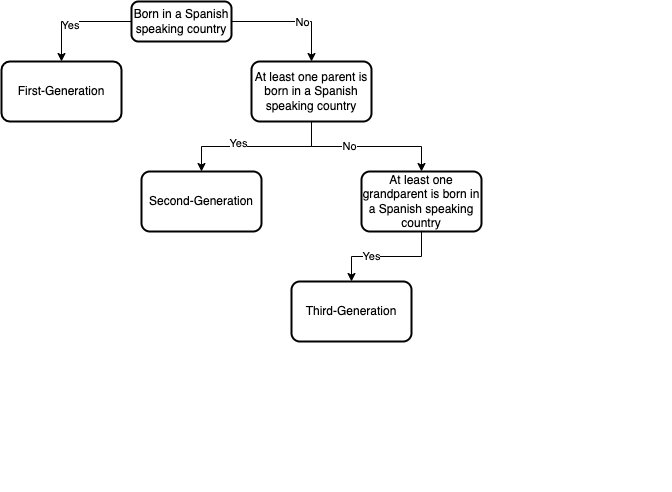
\includegraphics[width=\textwidth, height=9cm]{figure/diag.png} 
\label{fig:diag}
\end{figure}
\hfill%
\end{center}

My analysis depends on a sub sample of the US population, I show in table (\ref{tab:hispbygen}) that I have enough observations in each generation. Consistent with the literature on ethnic attrition among Hispanics, I find significant attrition among third-generation Hispanic immigrants.\footnote{In \citet{duncanIdentifyingLaterGenerationDescendants2018,duncanSocioeconomicIntegrationImmigrant2018, antmanEthnicAttritionObserved2016,antmanEthnicAttritionAssimilation2020}, the authors find substantial attrition among Hispanics.} These results are displayed in table (\ref{tab:hispbygen}): most first- and second-generation Hispanic immigrants self-reportedly identified as Hispanic. Among first-generation Hispanic immigrants, 96\% of the group self-reportedly identified as Hispanic. Among second-generation Hispanic immigrants, 95\% of the group self-reportedly identified as Hispanic. Attrition rates increase drastically after the second-generation, with 85\% of third-generation Hispanic immigrants identifying as Hispanic. That is more than three folds increase in attrition rates. Most of the attrition among third-generation Hispanics is driven by attrition among the children of inter-ethnic marriages.

\begin{table}[H]

\caption{Hispanic Self-identification by Generation \label{tab:hispbygen}}
\centering
\resizebox{\linewidth}{!}{
\fontsize{12}{14}\selectfont
\resizebox{\linewidth}{!}{
\begin{threeparttable}
\begin{tabular}[t]{>{}lcccc}
\toprule
  & Self-identify as Hispanic & Self-identify as non-Hispanic & \% Self-identify as Hispanic & \% Self-identify as non-Hispanic\\
\midrule
\textbf{1st Gen.} & 114657 & 5121 & 0.96 & 0.04\\
\textbf{2nd Gen.} & 712916 & 48534 & 0.94 & 0.06\\
\hspace{1em}\textbf{Hispanic on:} &  &  &  & \\
\hspace{1em}\hspace{1em}\textbf{Both Sides} & 516551 & 19318 & 0.96 & 0.04\\
\hspace{1em}\hspace{1em}\textbf{One Side} & 196365 & 29216 & 0.87 & 0.13\\
\addlinespace
\textbf{3rd Gen.} & 209206 & 45493 & 0.82 & 0.18\\
\hspace{1em}\textbf{Hispanic on:} &  &  &  & \\
\hspace{1em}\hspace{1em}\textbf{Both Sides} & 55401 & 2245 & 0.96 & 0.04\\
\hspace{1em}\hspace{1em}\textbf{One Side} & 52879 & 17371 & 0.75 & 0.25\\
\bottomrule
\end{tabular}
\begin{tablenotes}
\item[1] The samples include children ages 17 and below who live in intact families. First-generation Hispanic immigrant children that were born in a Spanish speaking county. Native born second-generation Hispanic immigrant children with at least one parent born in a Spanish speaking country. Finally, native born third-generation Hispanic immigrant children with native born parents and at least one grandparent born in a Spanish speaking country.
\item[2] Data source is the 2004-2021 Current Population Survey.
\end{tablenotes}
\end{threeparttable}}}
\end{table}


\begin{figure}[H]
\begin{center}

\caption{Bias and Self-reported Hispanic Identity in the Least and Most Biased Places}

% first
\begin{subfigure}{.9\textwidth}
\caption{Skin Tone Implicit Association Bias Over Time}
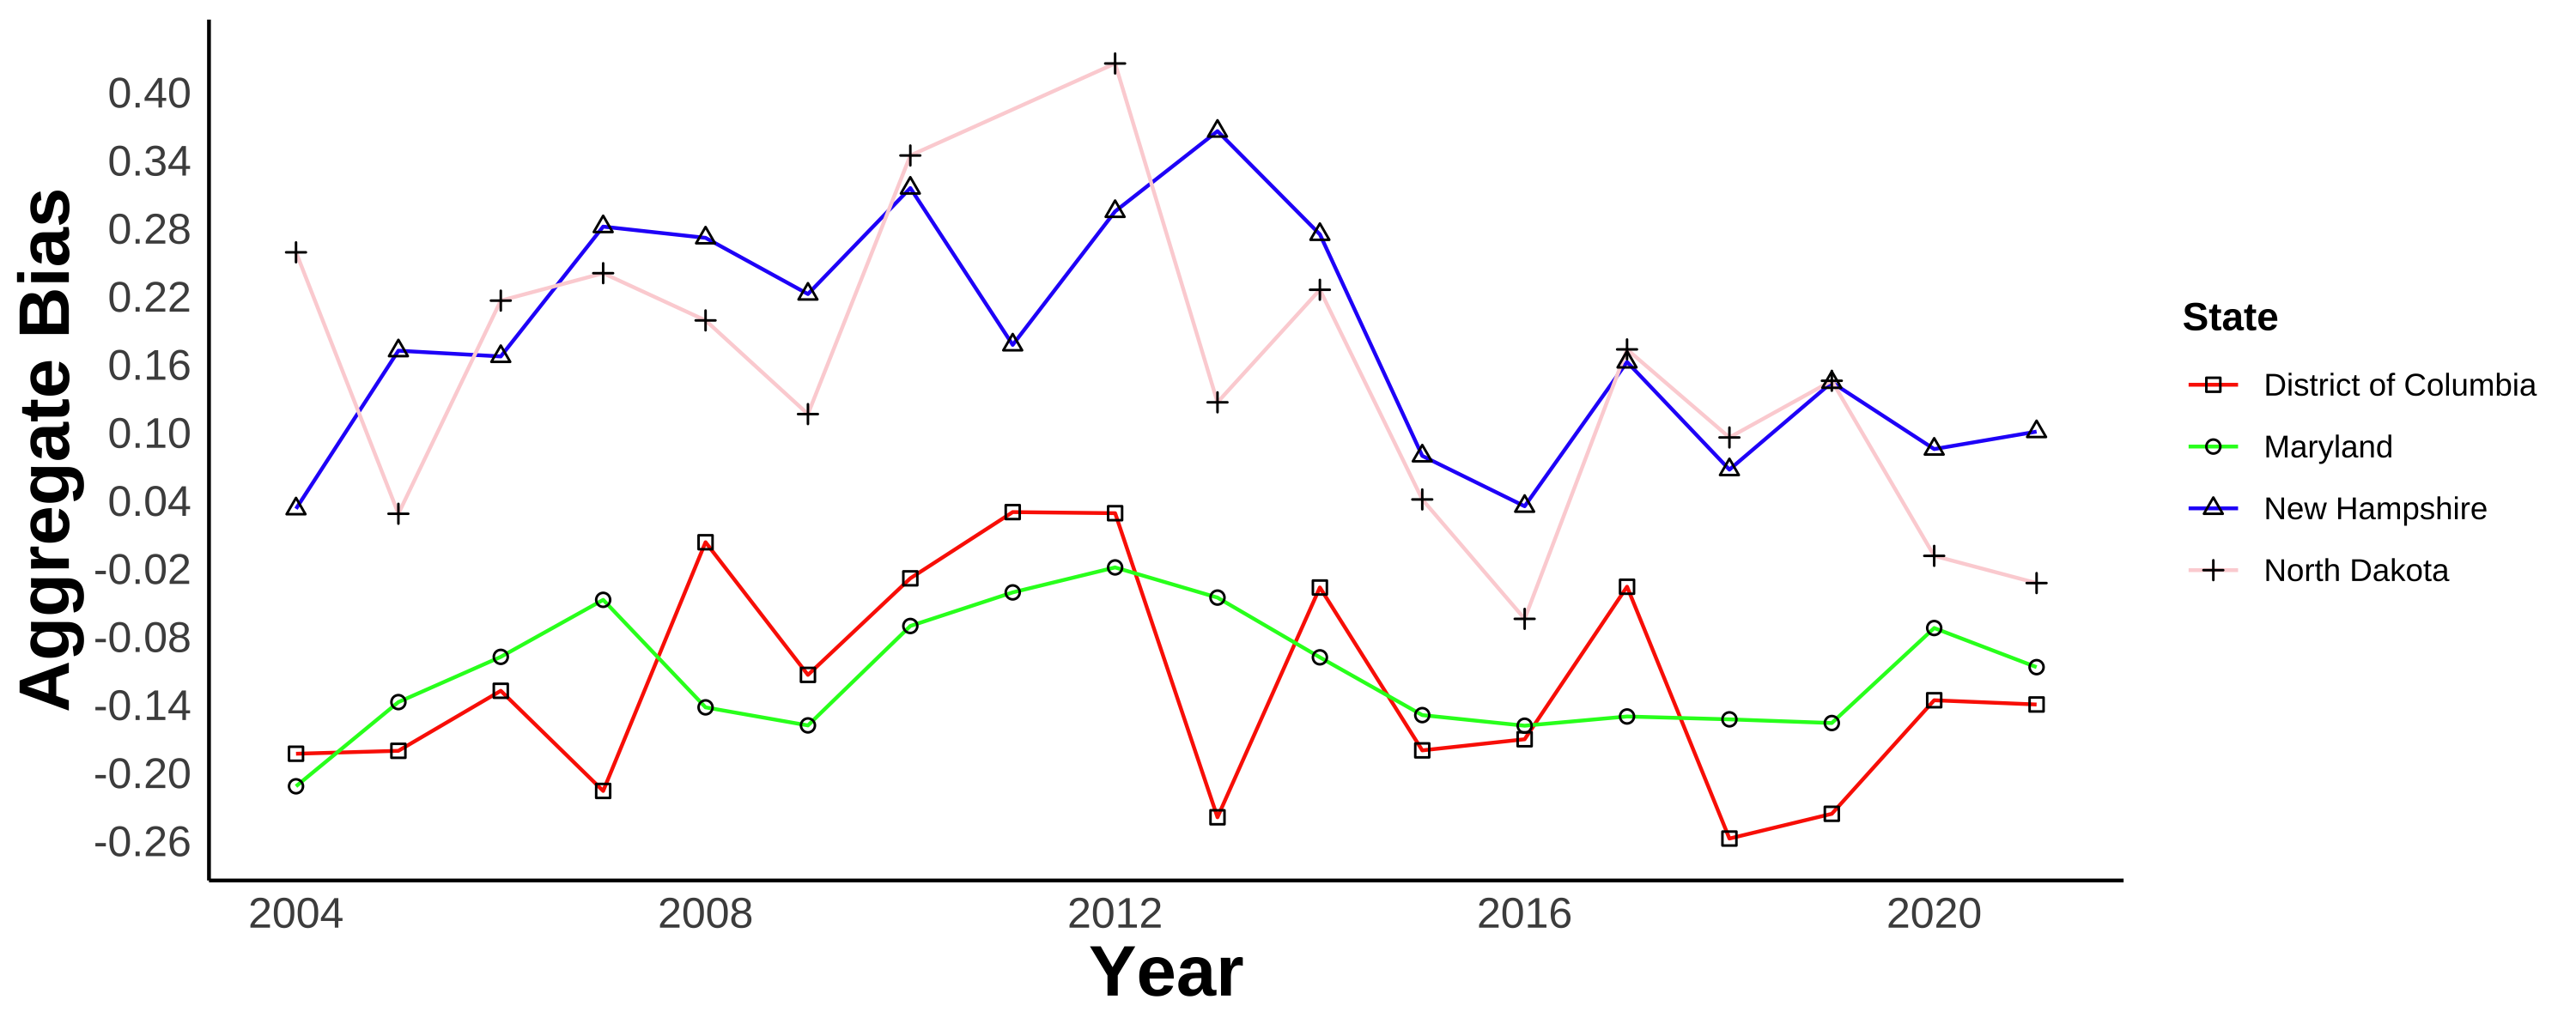
\includegraphics[width=.9\linewidth]{figure/Bias_twostates.png} 
\label{fig:skiniat}
\end{subfigure}
% Second
\begin{subfigure}{.9\textwidth}
\caption{Self-reported Hispanic Identity Over Time}
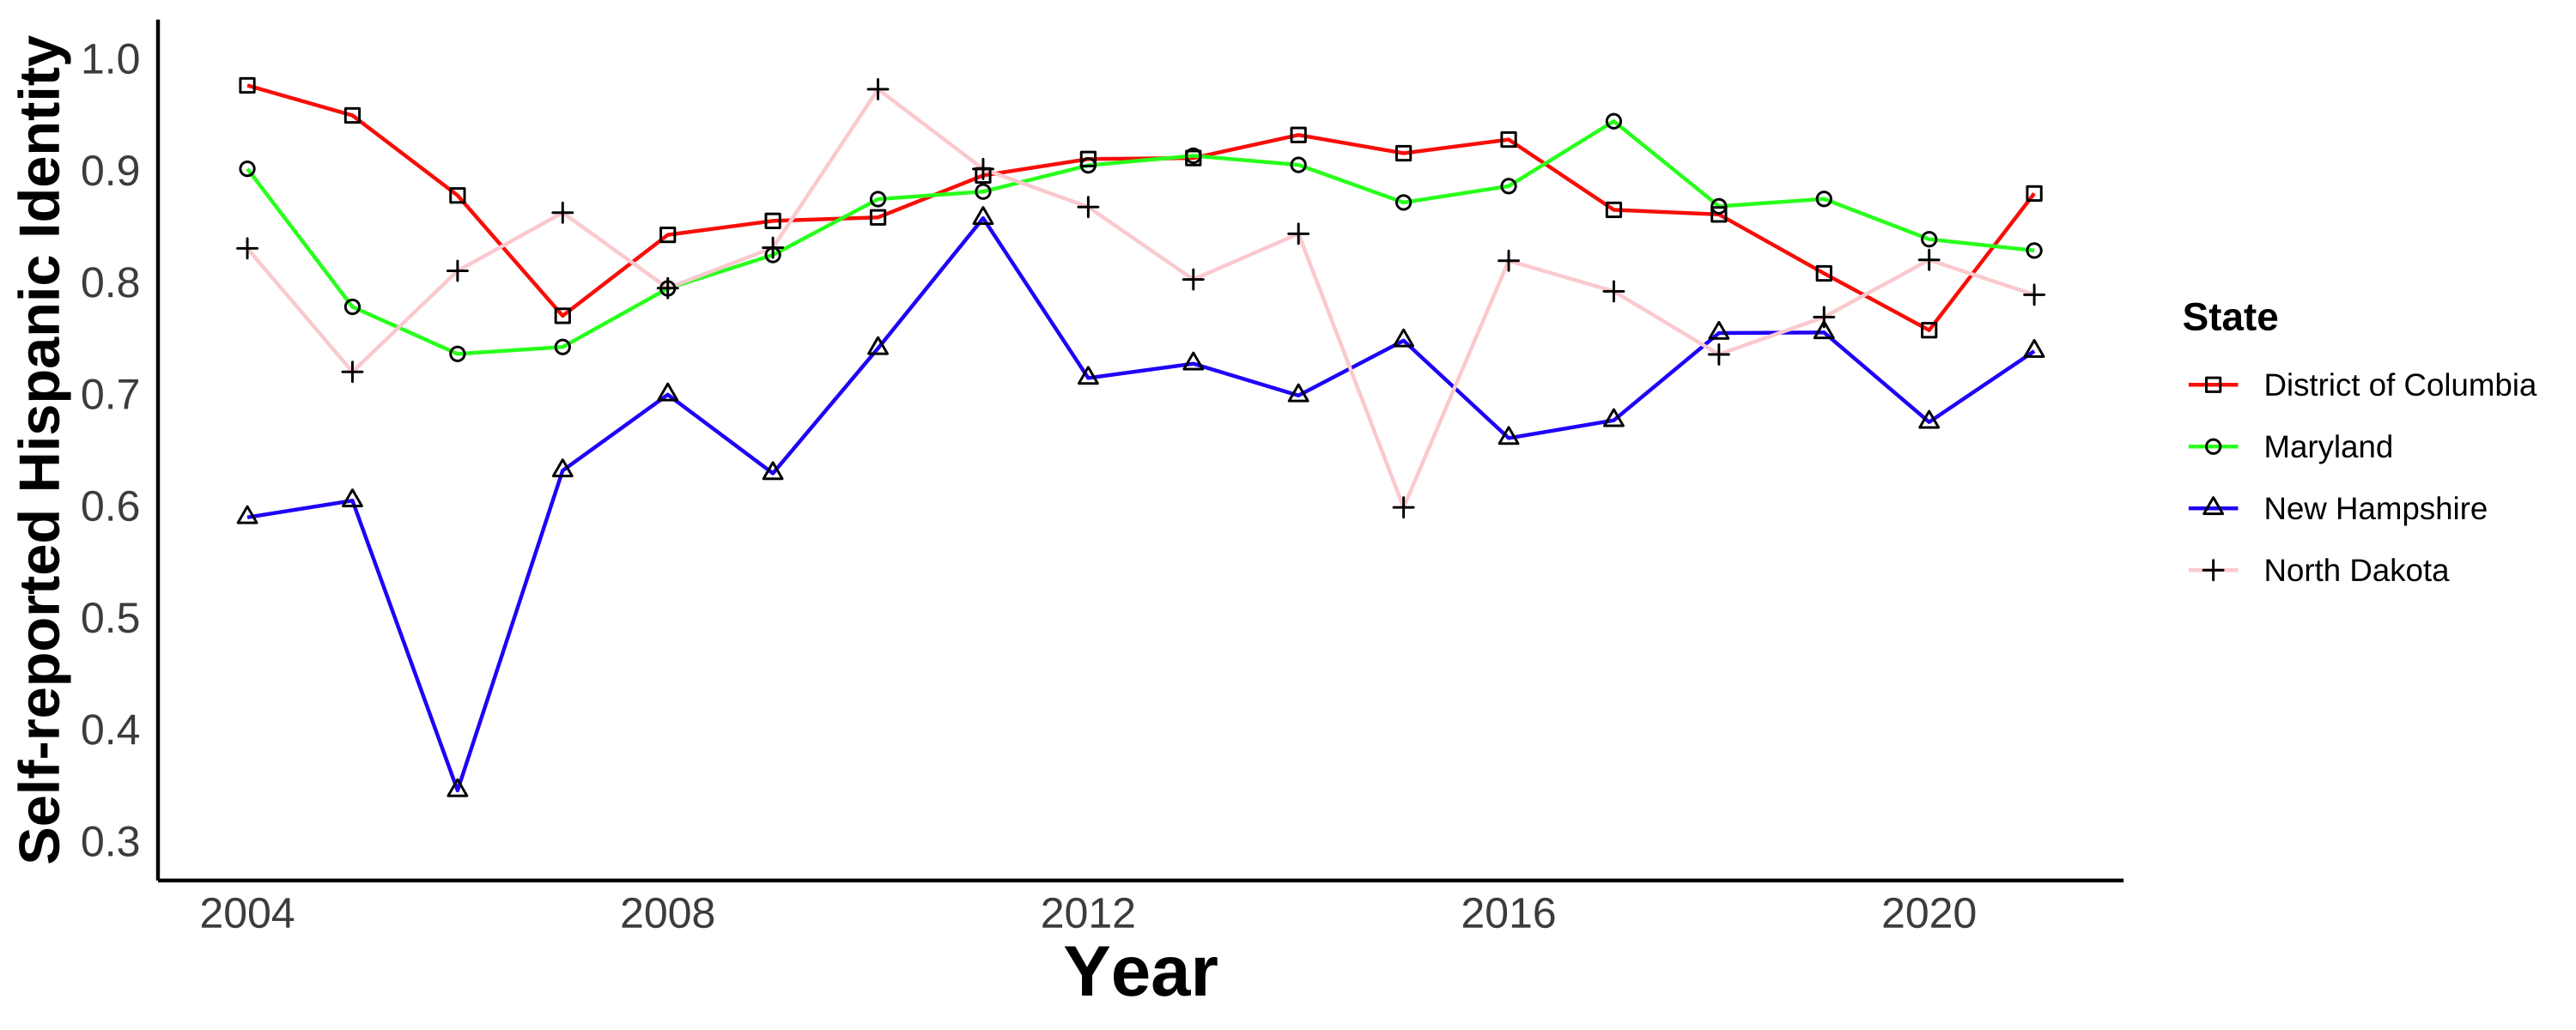
\includegraphics[width=.9\linewidth]{figure/Bias_twostates-hisp.png} 
\label{fig:hispanic-twostates}
\end{subfigure}
\flushleft\footnotesize{\note{These two panels show the trends in implicit bias (panel a) and self-reported Hispanic identity among Hispanic immigrants (panel b) of the least and most biased places in the data. The District of Colombia is the least biased geographical area, and North Dakota is the most biased. The bias units are in standard deviations. Self-reported Hispanic identity is among first, second, and third-generation Hispanic immigrants aged 17 and younger still living in intact families.}\\
\note{Bias data is from the 2004-2021 Harvard's Project Implicit Association Test scores. Identity data is from the 2004-2021 Current Population Survey (CPS).}}
\end{center}
\end{figure}

\pagebreak
\newpage

\begin{center}
\begin{figure}[H]
\caption{Maps of State-level Implicit Association Test Bias Over Time Measure with Census Division Regional Boundaries}
\label{fig:skiniat-maps}
% first
\begin{subfigure}{.3\textwidth}
\caption{State-level Bias in 2004}
\centering
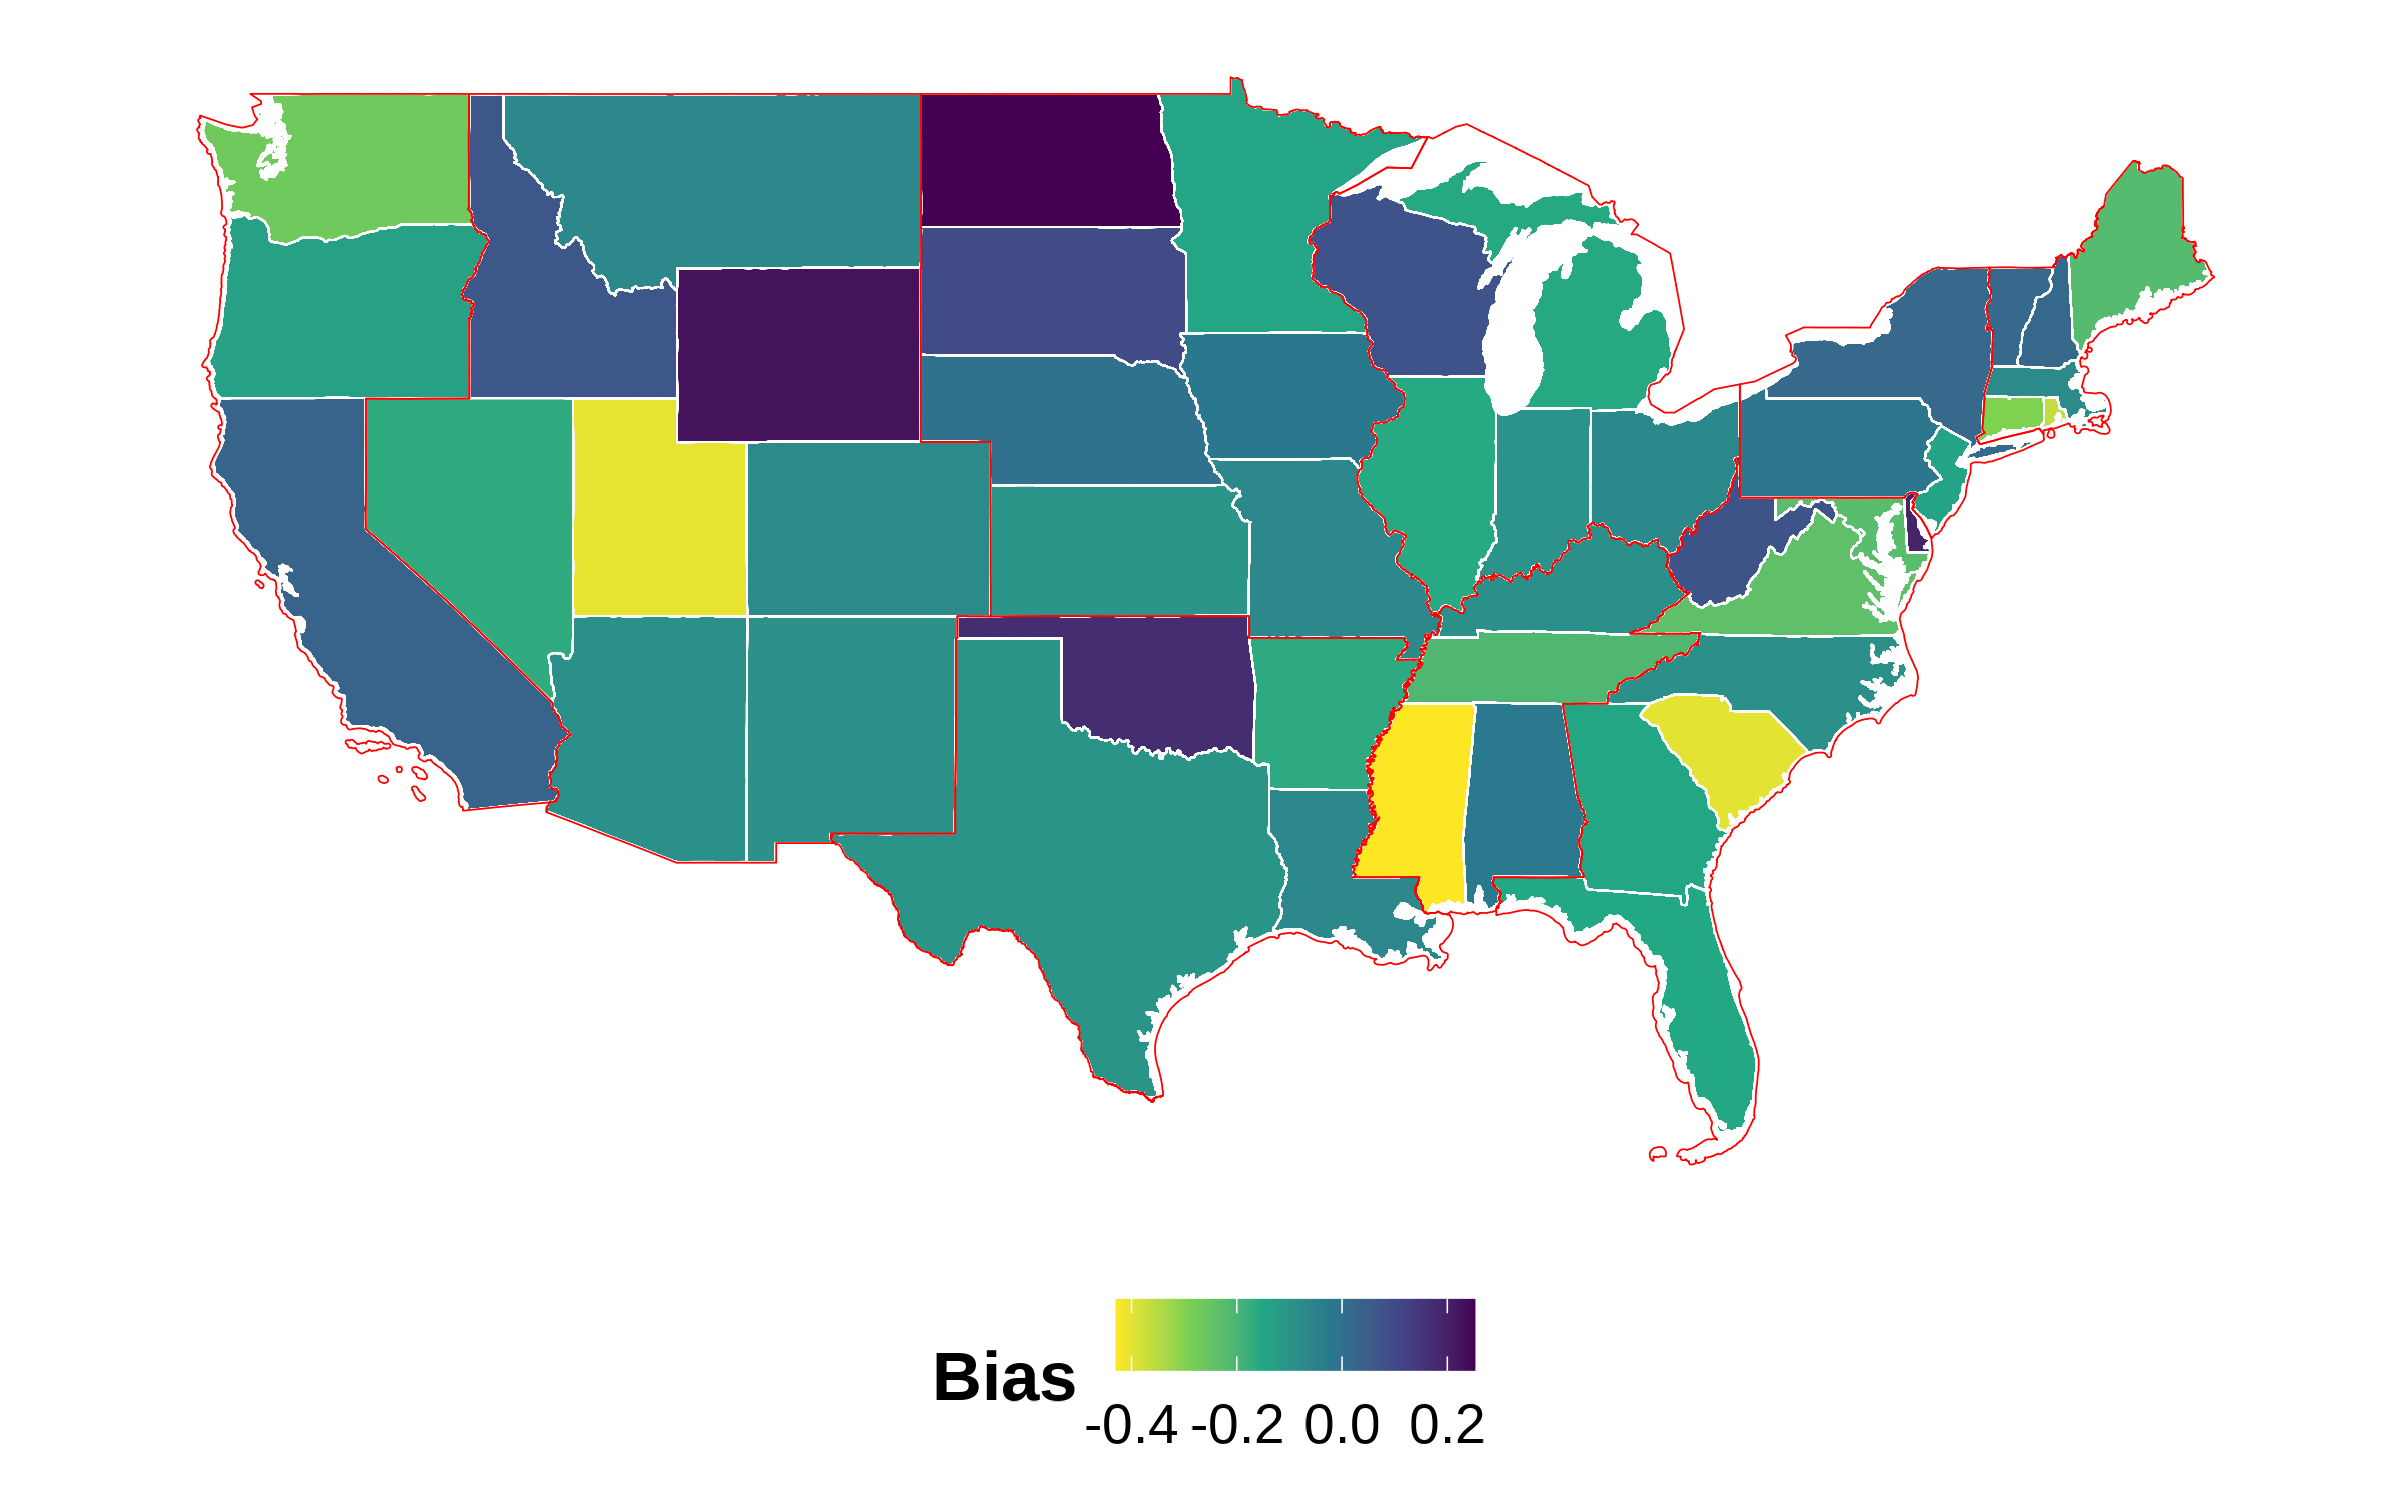
\includegraphics[width=\linewidth]{figure/2004skinmap.png} 
\label{fig:skiniat-map-2004}
\end{subfigure}
\hfill%
% Second
\begin{subfigure}{.3\textwidth}
\caption{State-level Bias in 2006}
\centering
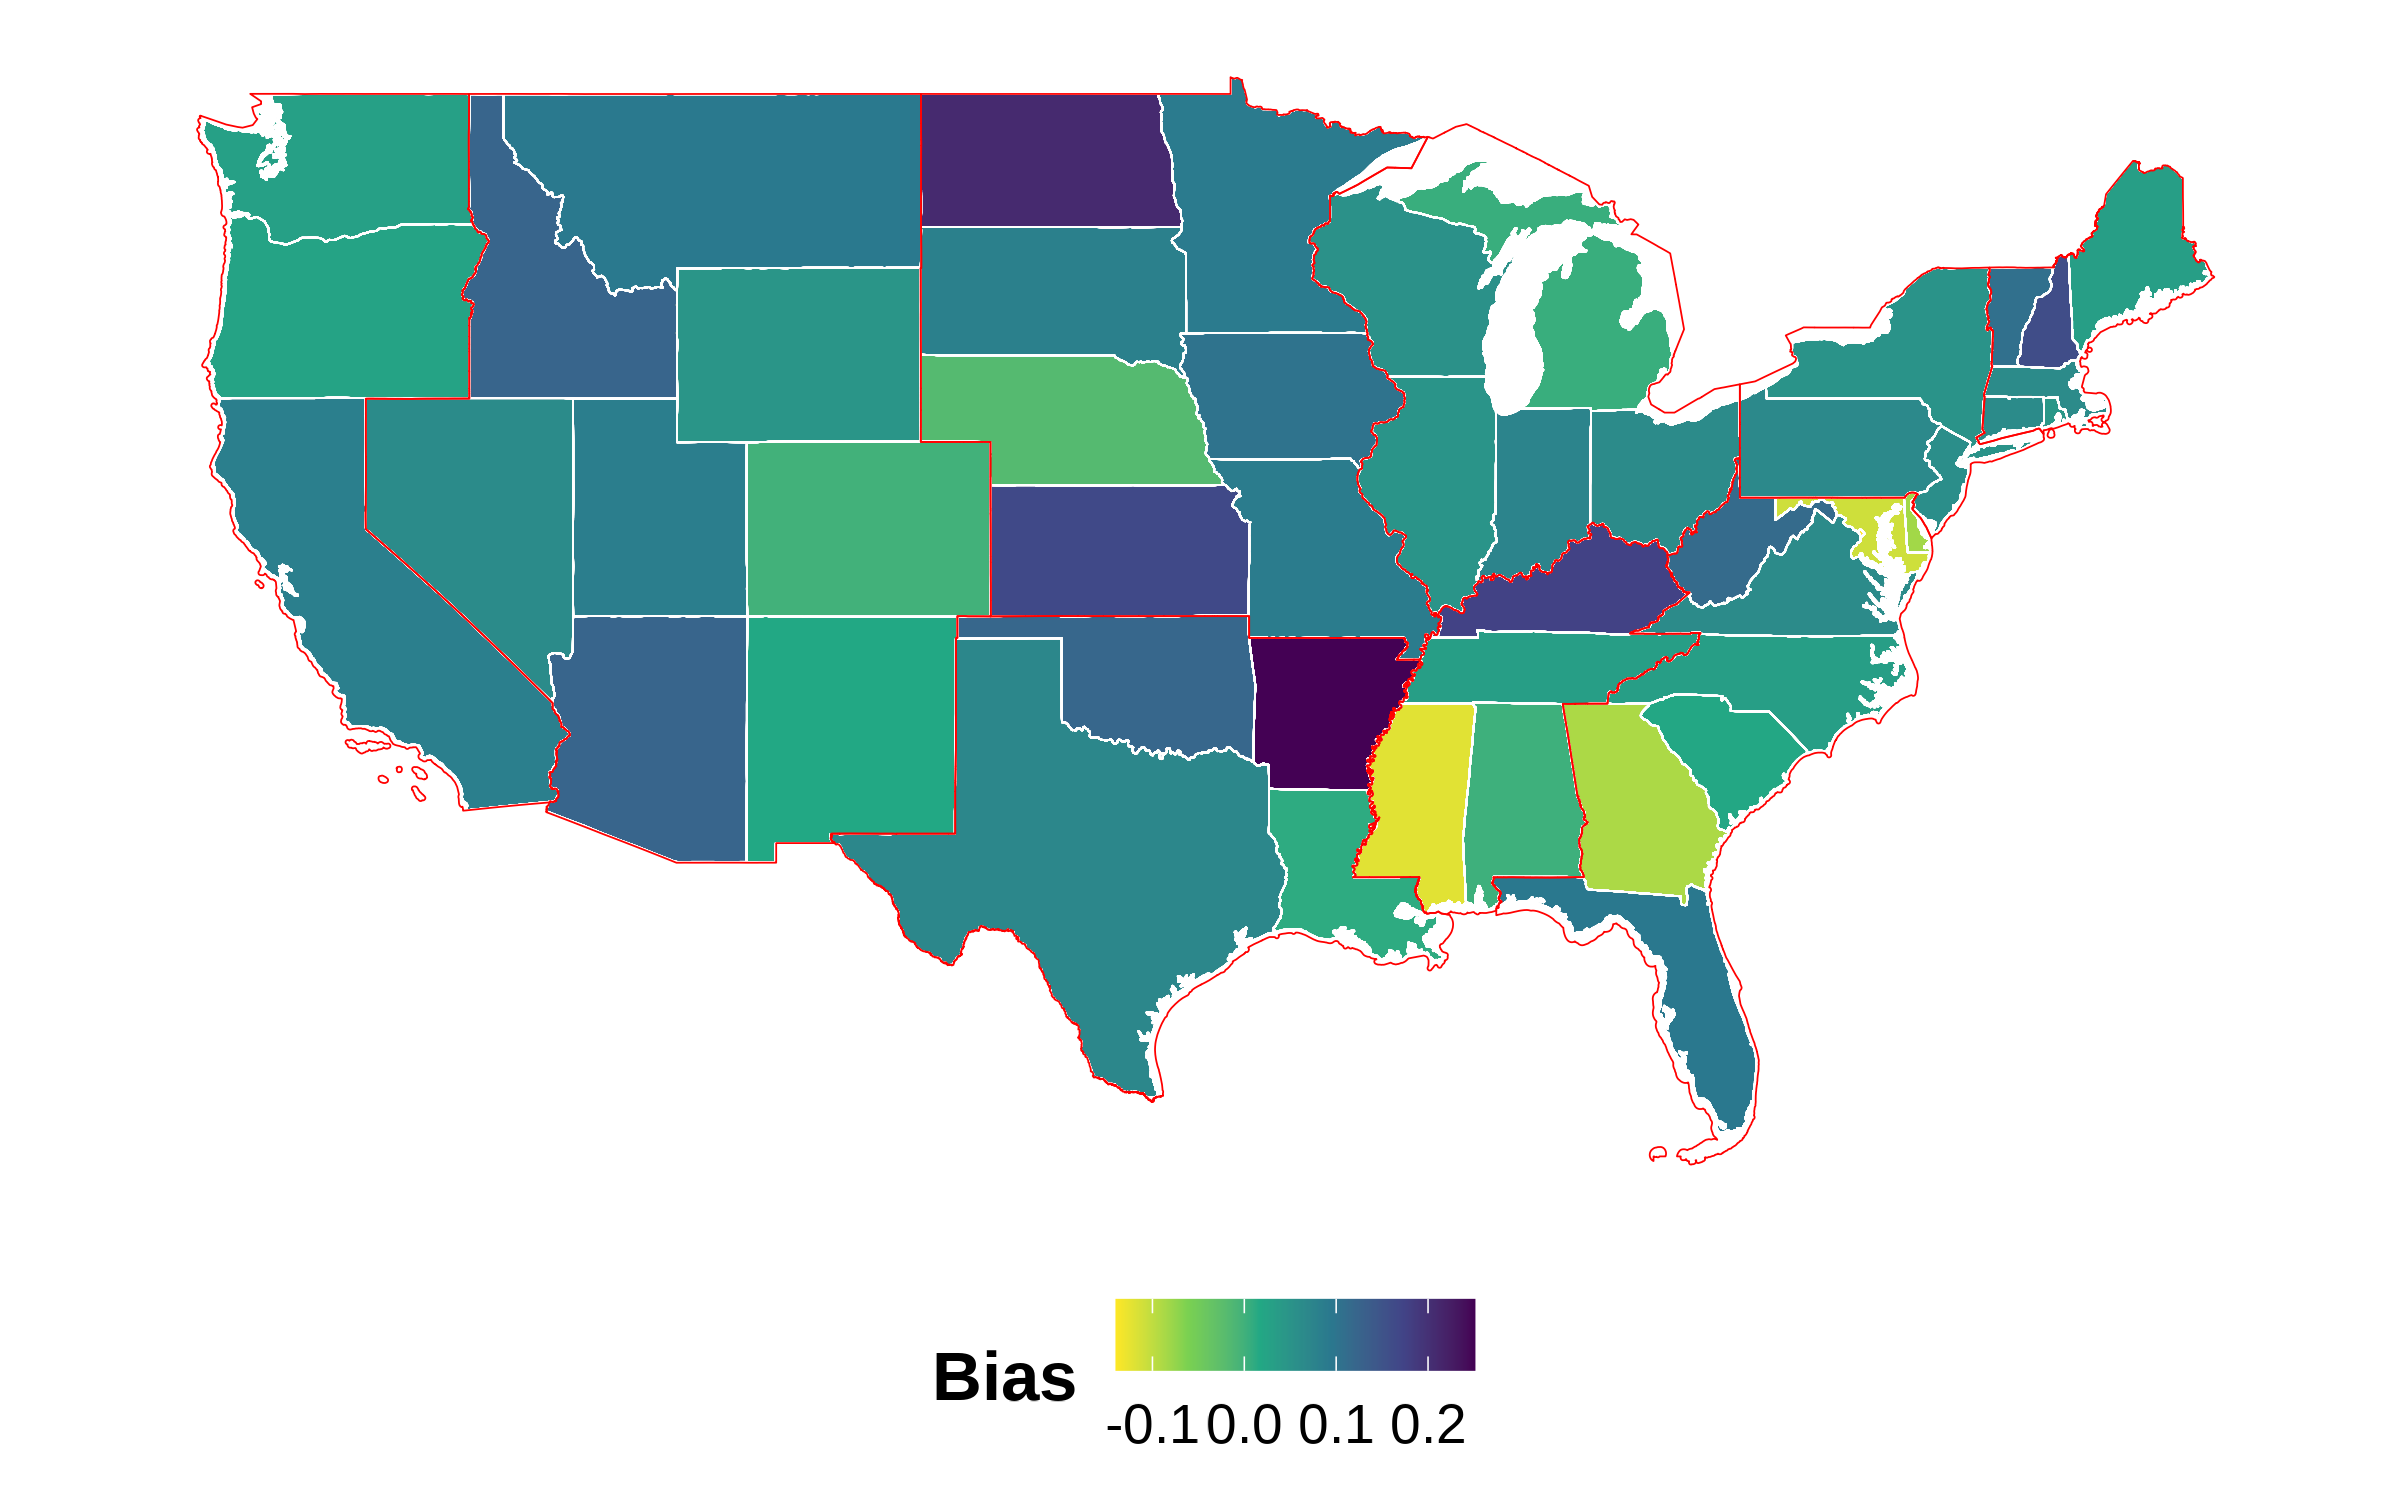
\includegraphics[width=\linewidth]{figure/2006skinmap.png} 
\label{fig:skiniat-map-2006}
\end{subfigure}
\hfill%
% third
\begin{subfigure}{.3\textwidth}
\caption{State-level Bias in 2008}
\centering
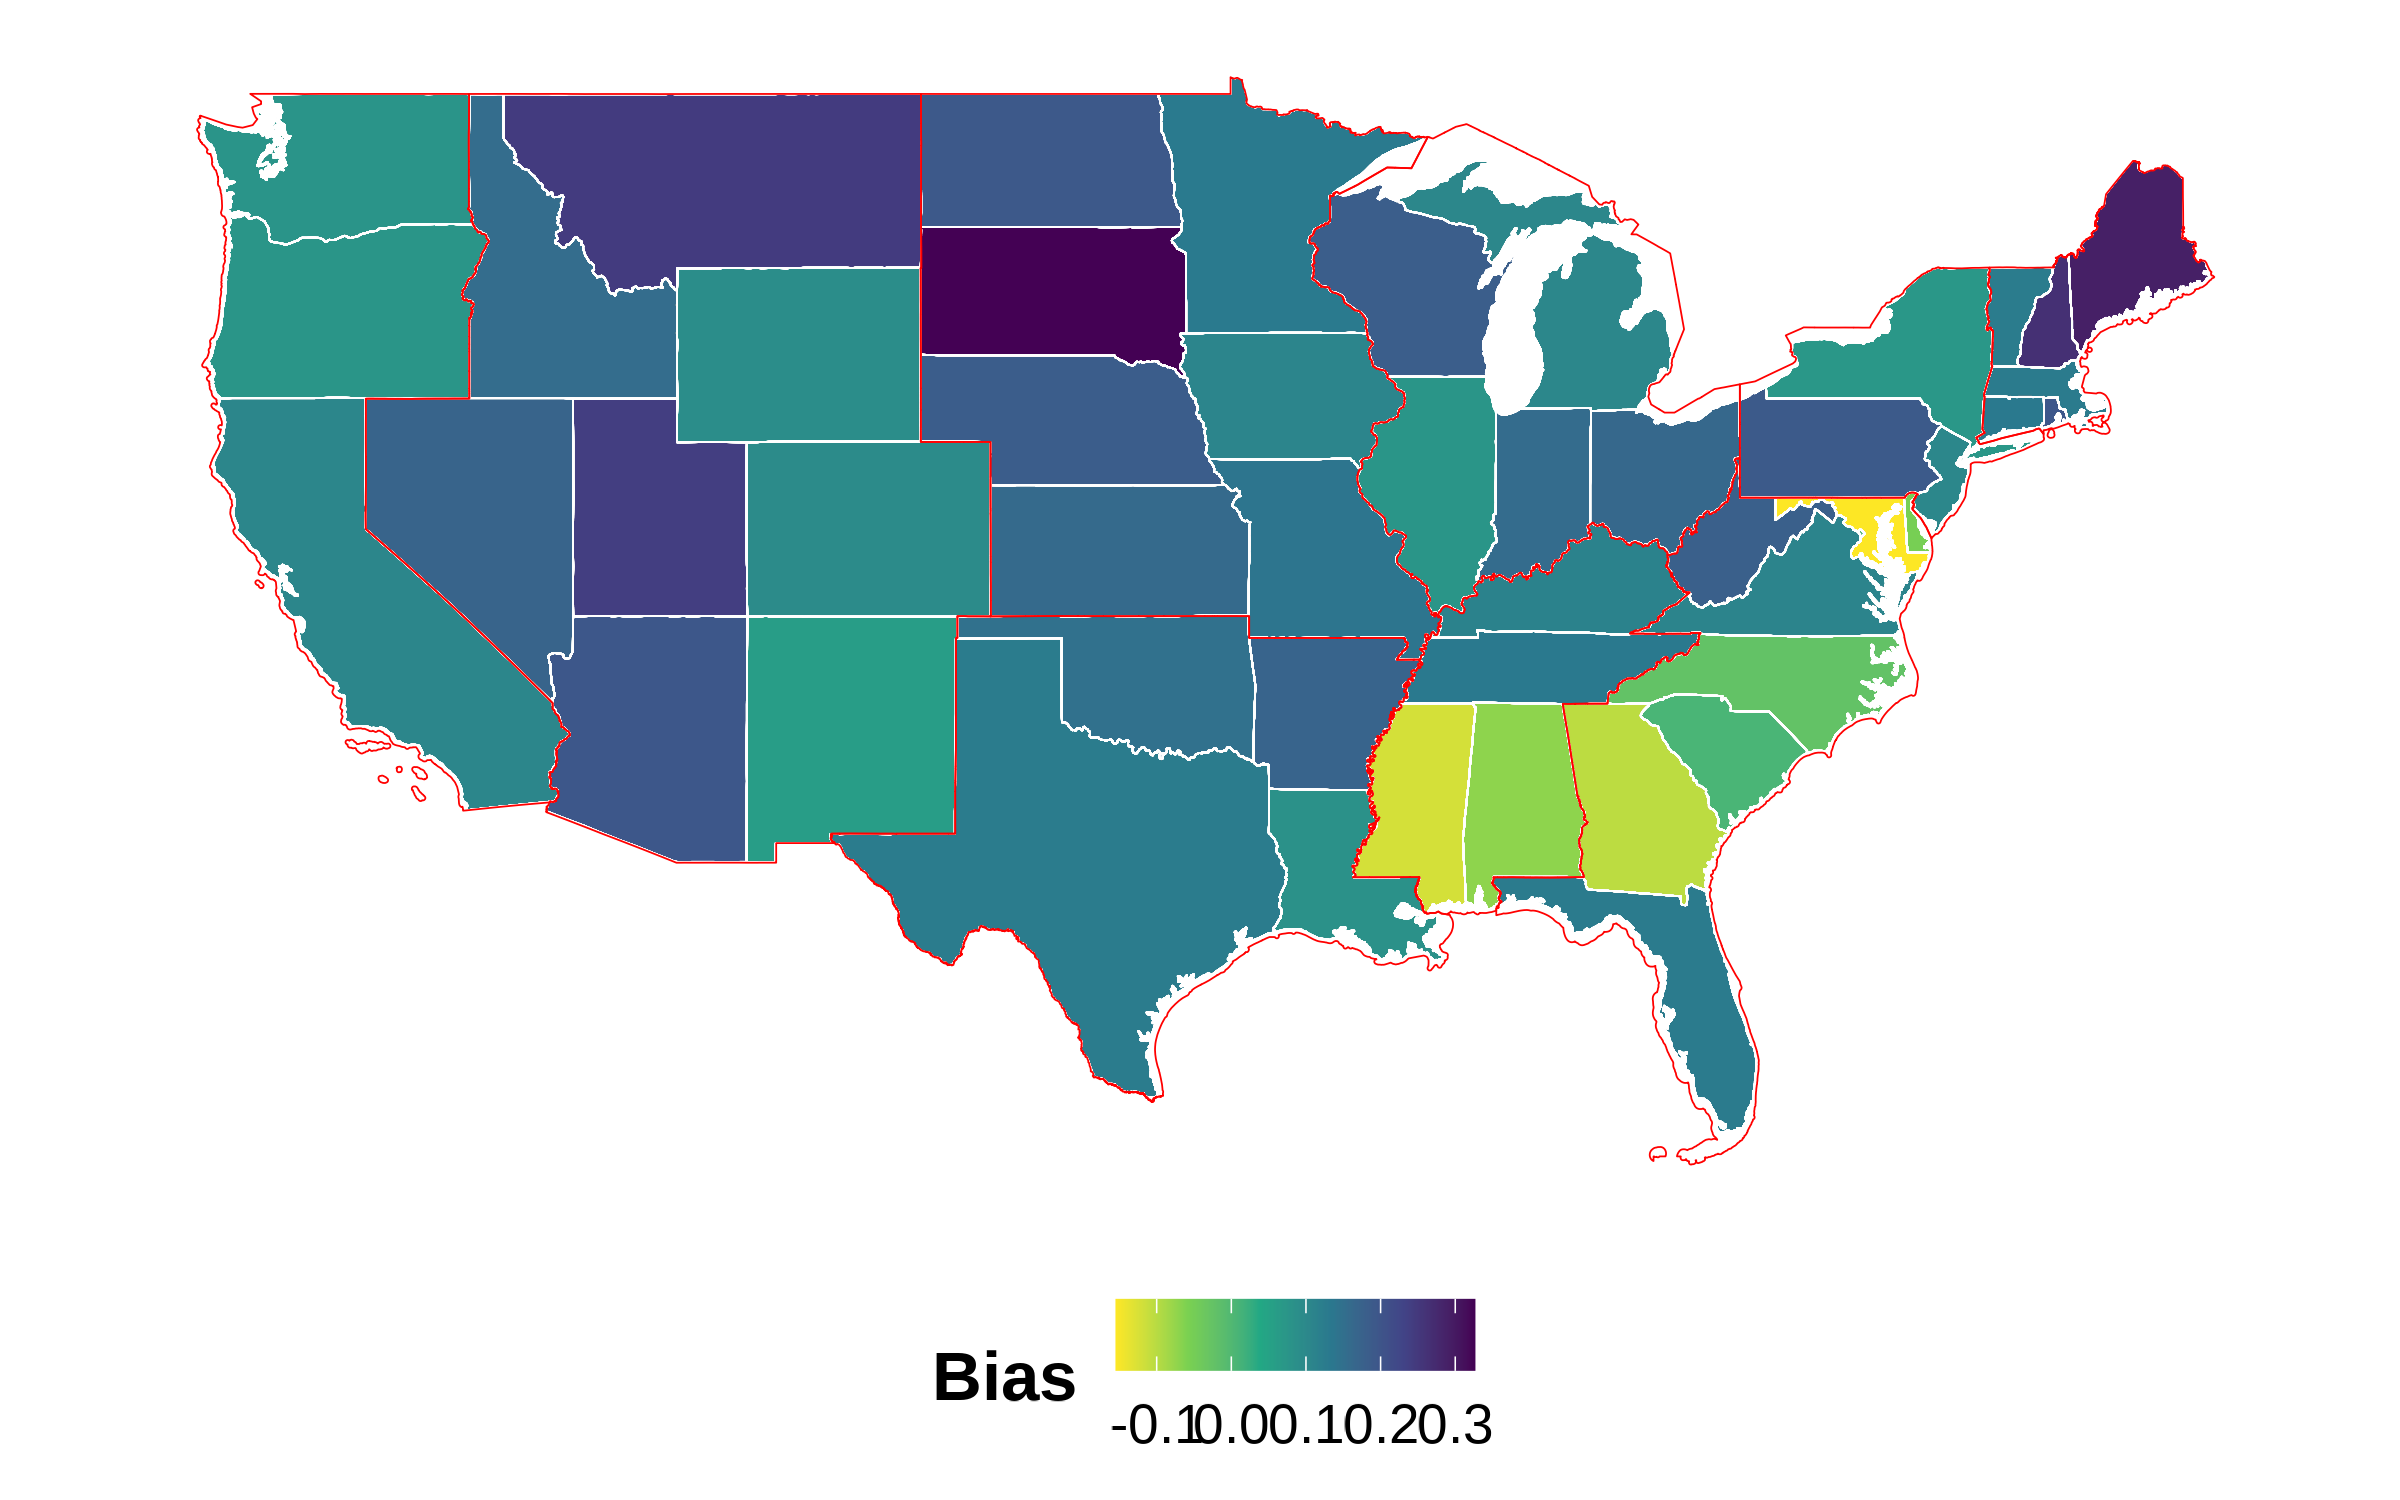
\includegraphics[width=\linewidth]{figure/2008skinmap.png} 
\label{fig:skiniat-map-2008}
\end{subfigure}
\hfill%
% fourth
\begin{subfigure}{.3\textwidth}
\caption{State-level Bias in 2010}
\centering
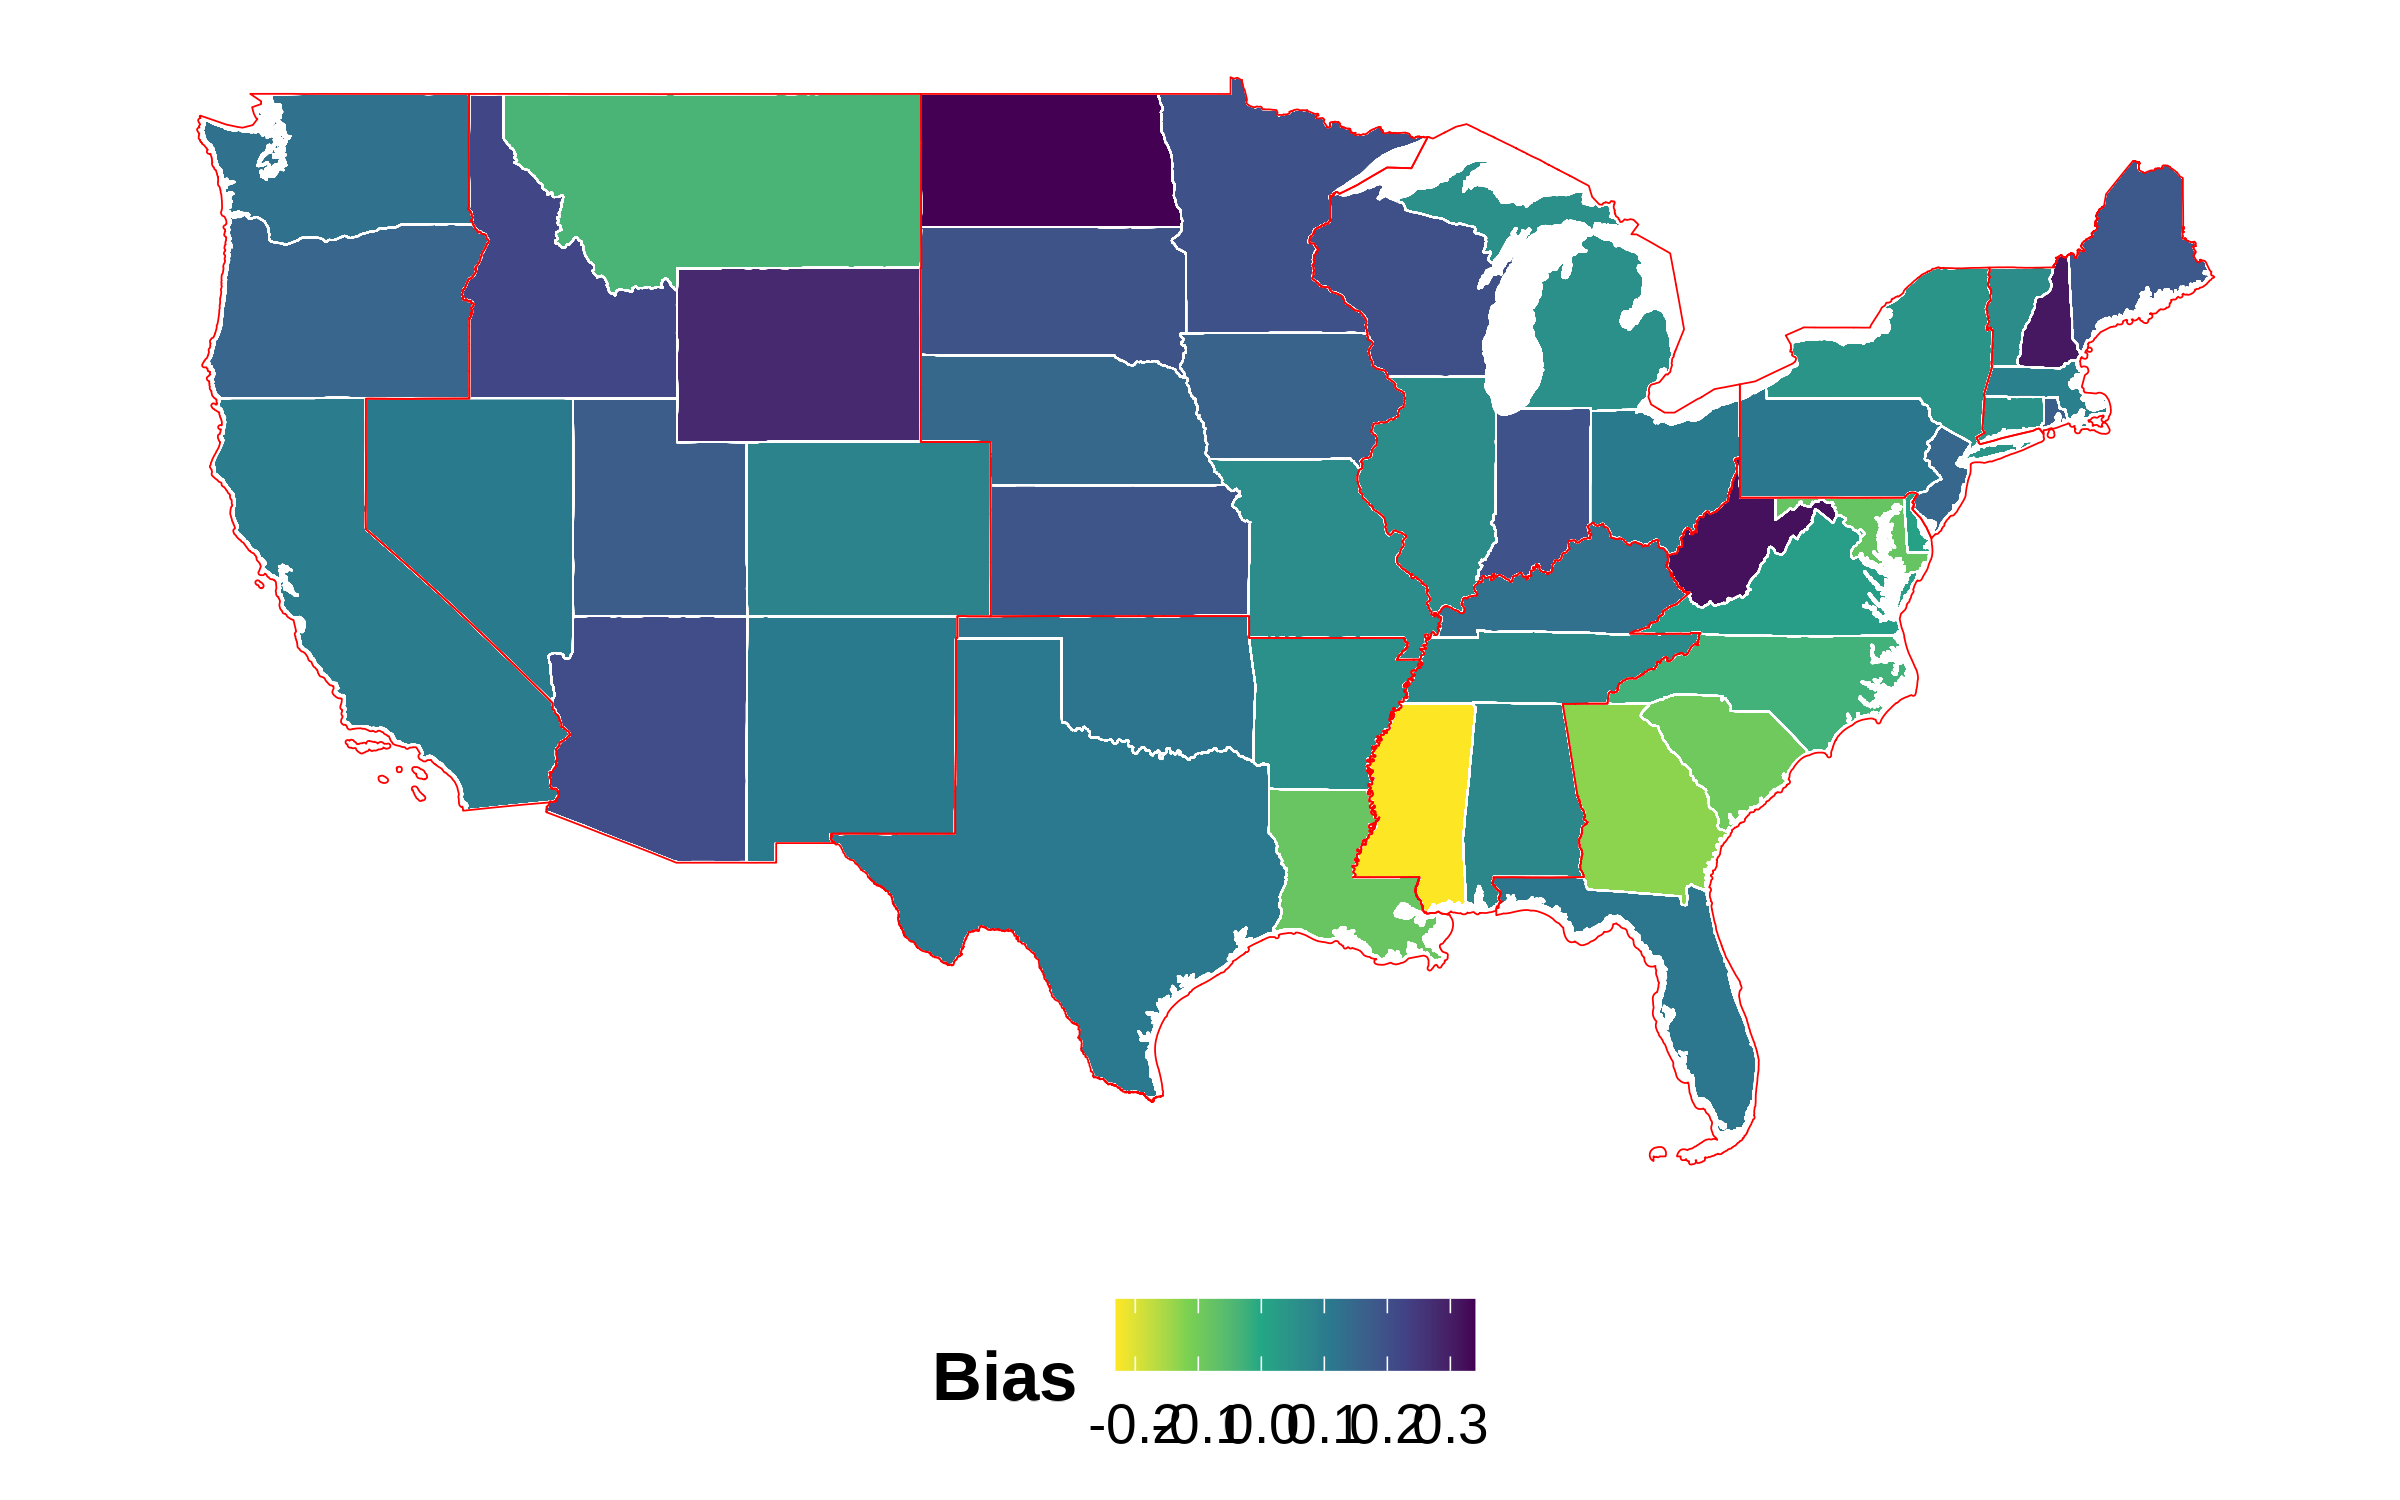
\includegraphics[width=\linewidth]{figure/2010skinmap.png} 
\label{fig:skiniat-map-2010}
\end{subfigure}
\hfill%
% fifth
\begin{subfigure}{.3\textwidth}
\caption{State-level Bias in 2012}
\centering
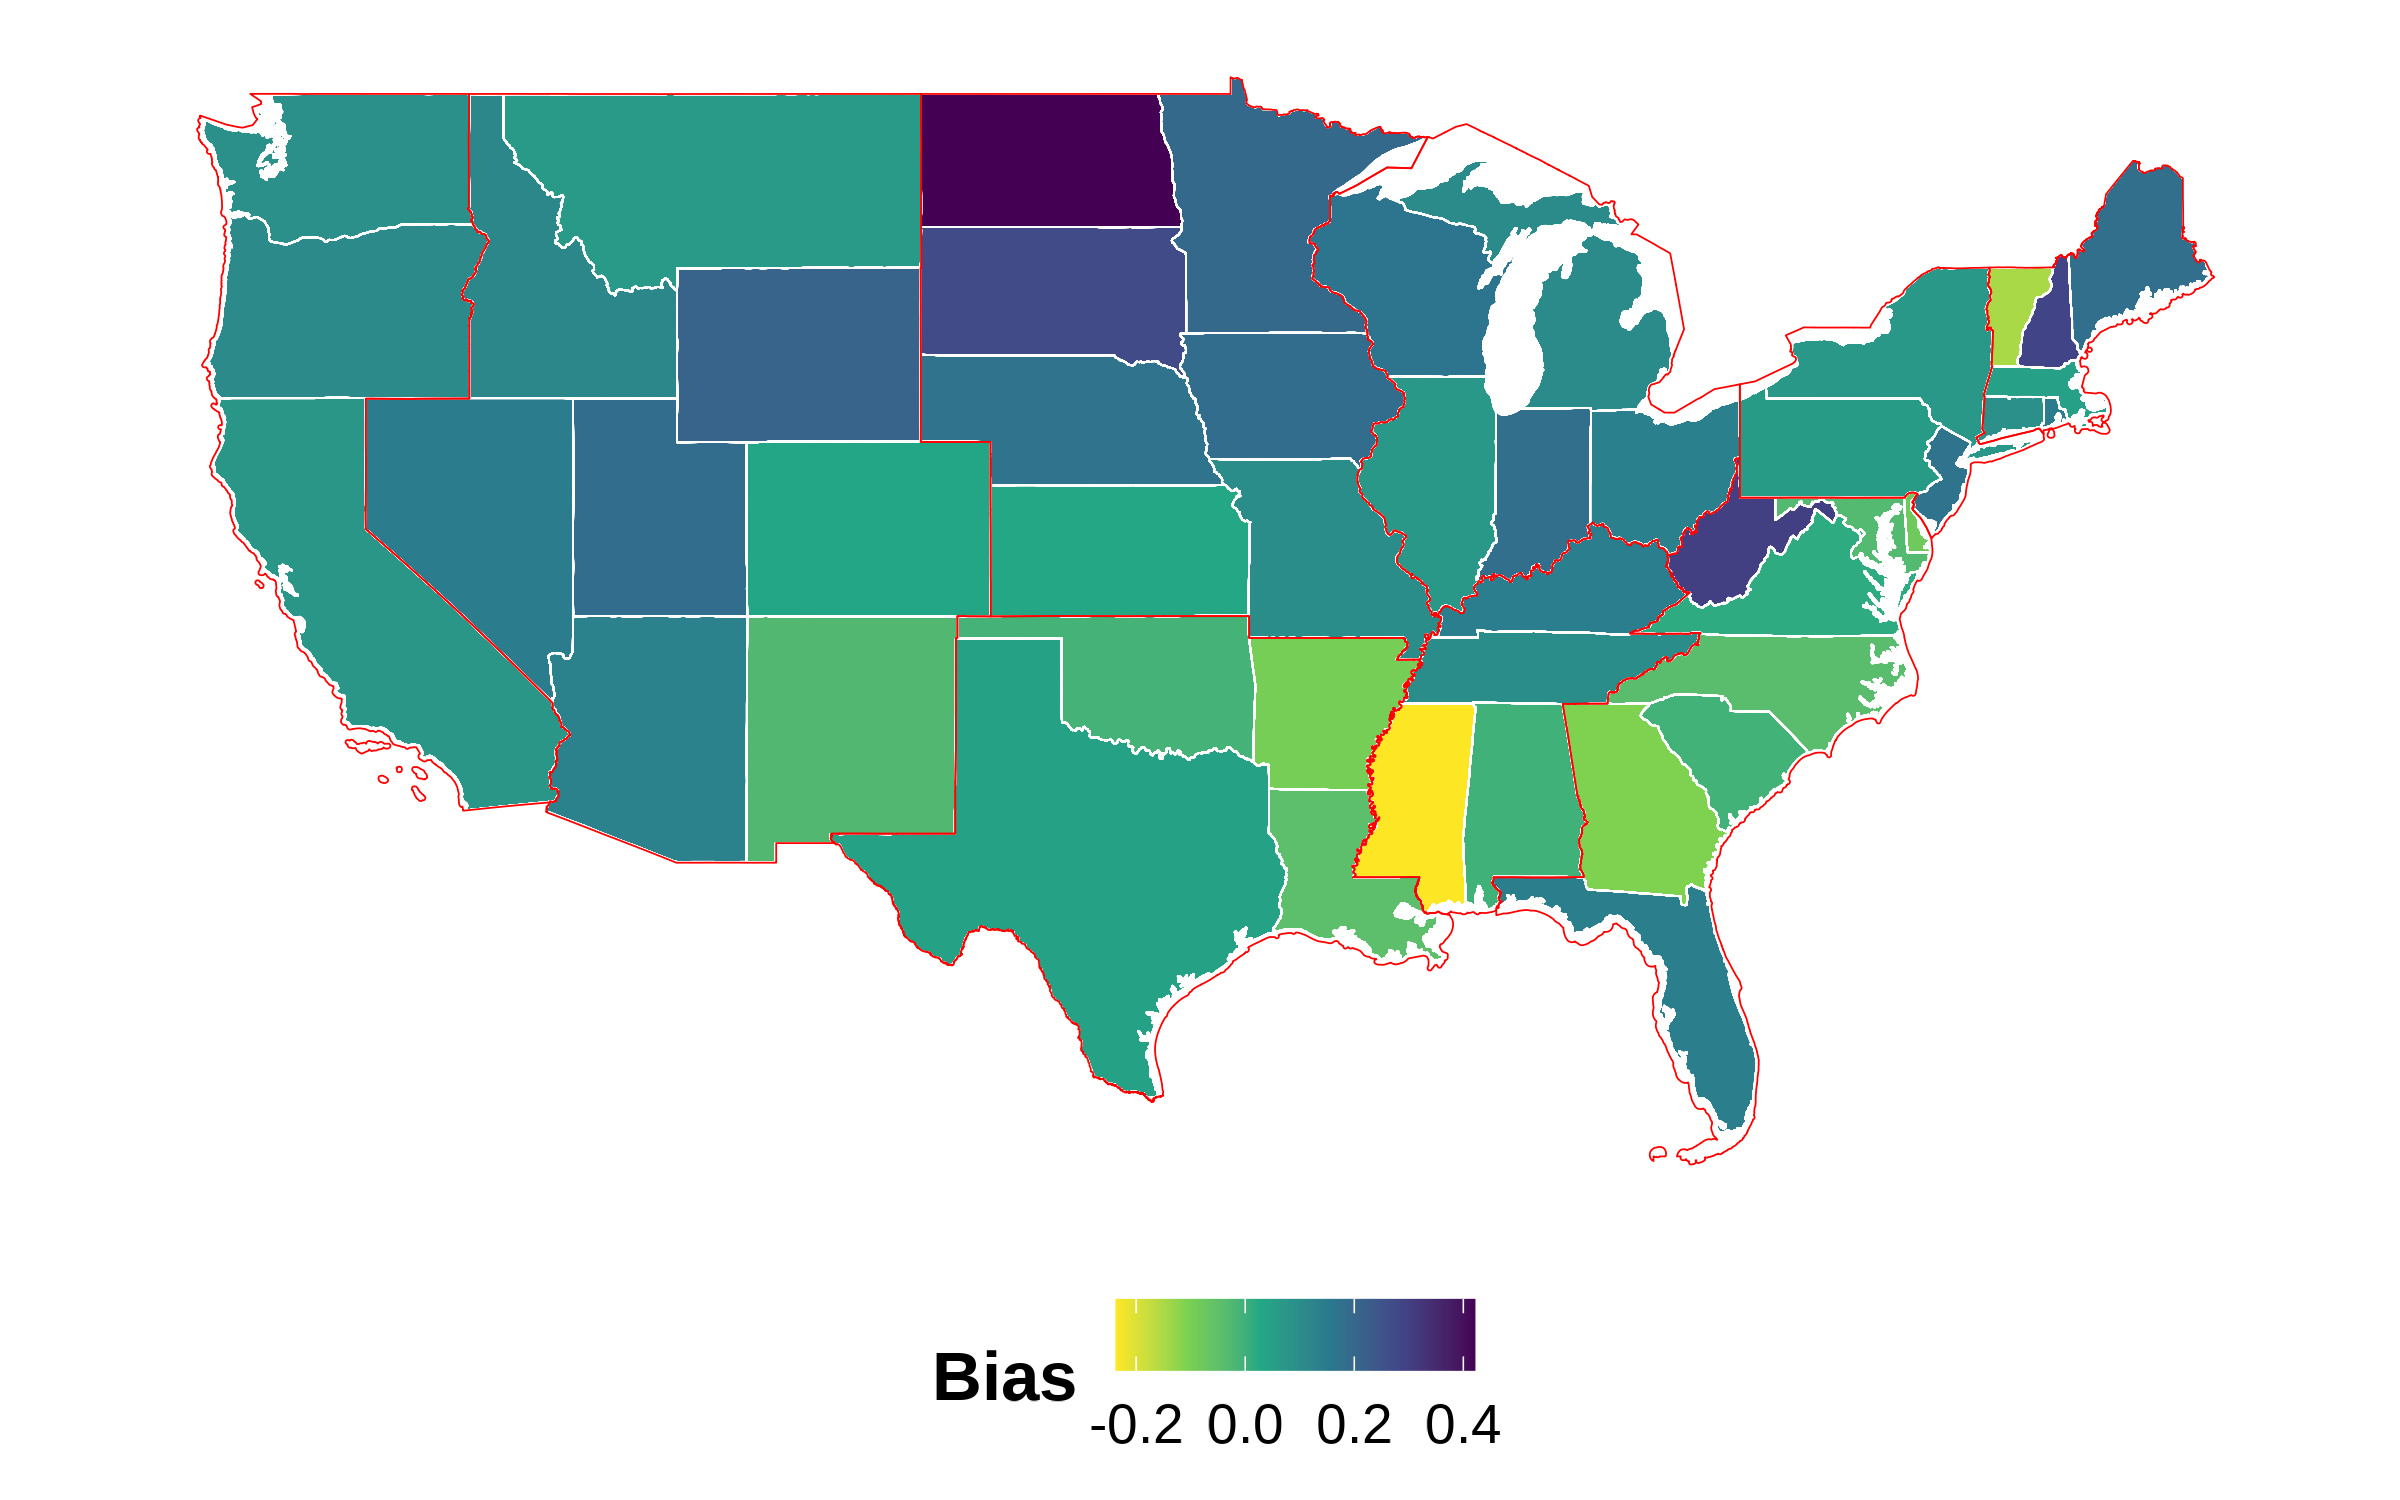
\includegraphics[width=\linewidth]{figure/2012skinmap.png} 
\label{fig:skiniat-map-2012}
\end{subfigure}
\hfill%
% sixth
\begin{subfigure}{.3\textwidth}
\caption{State-level Bias in 2014}
\centering
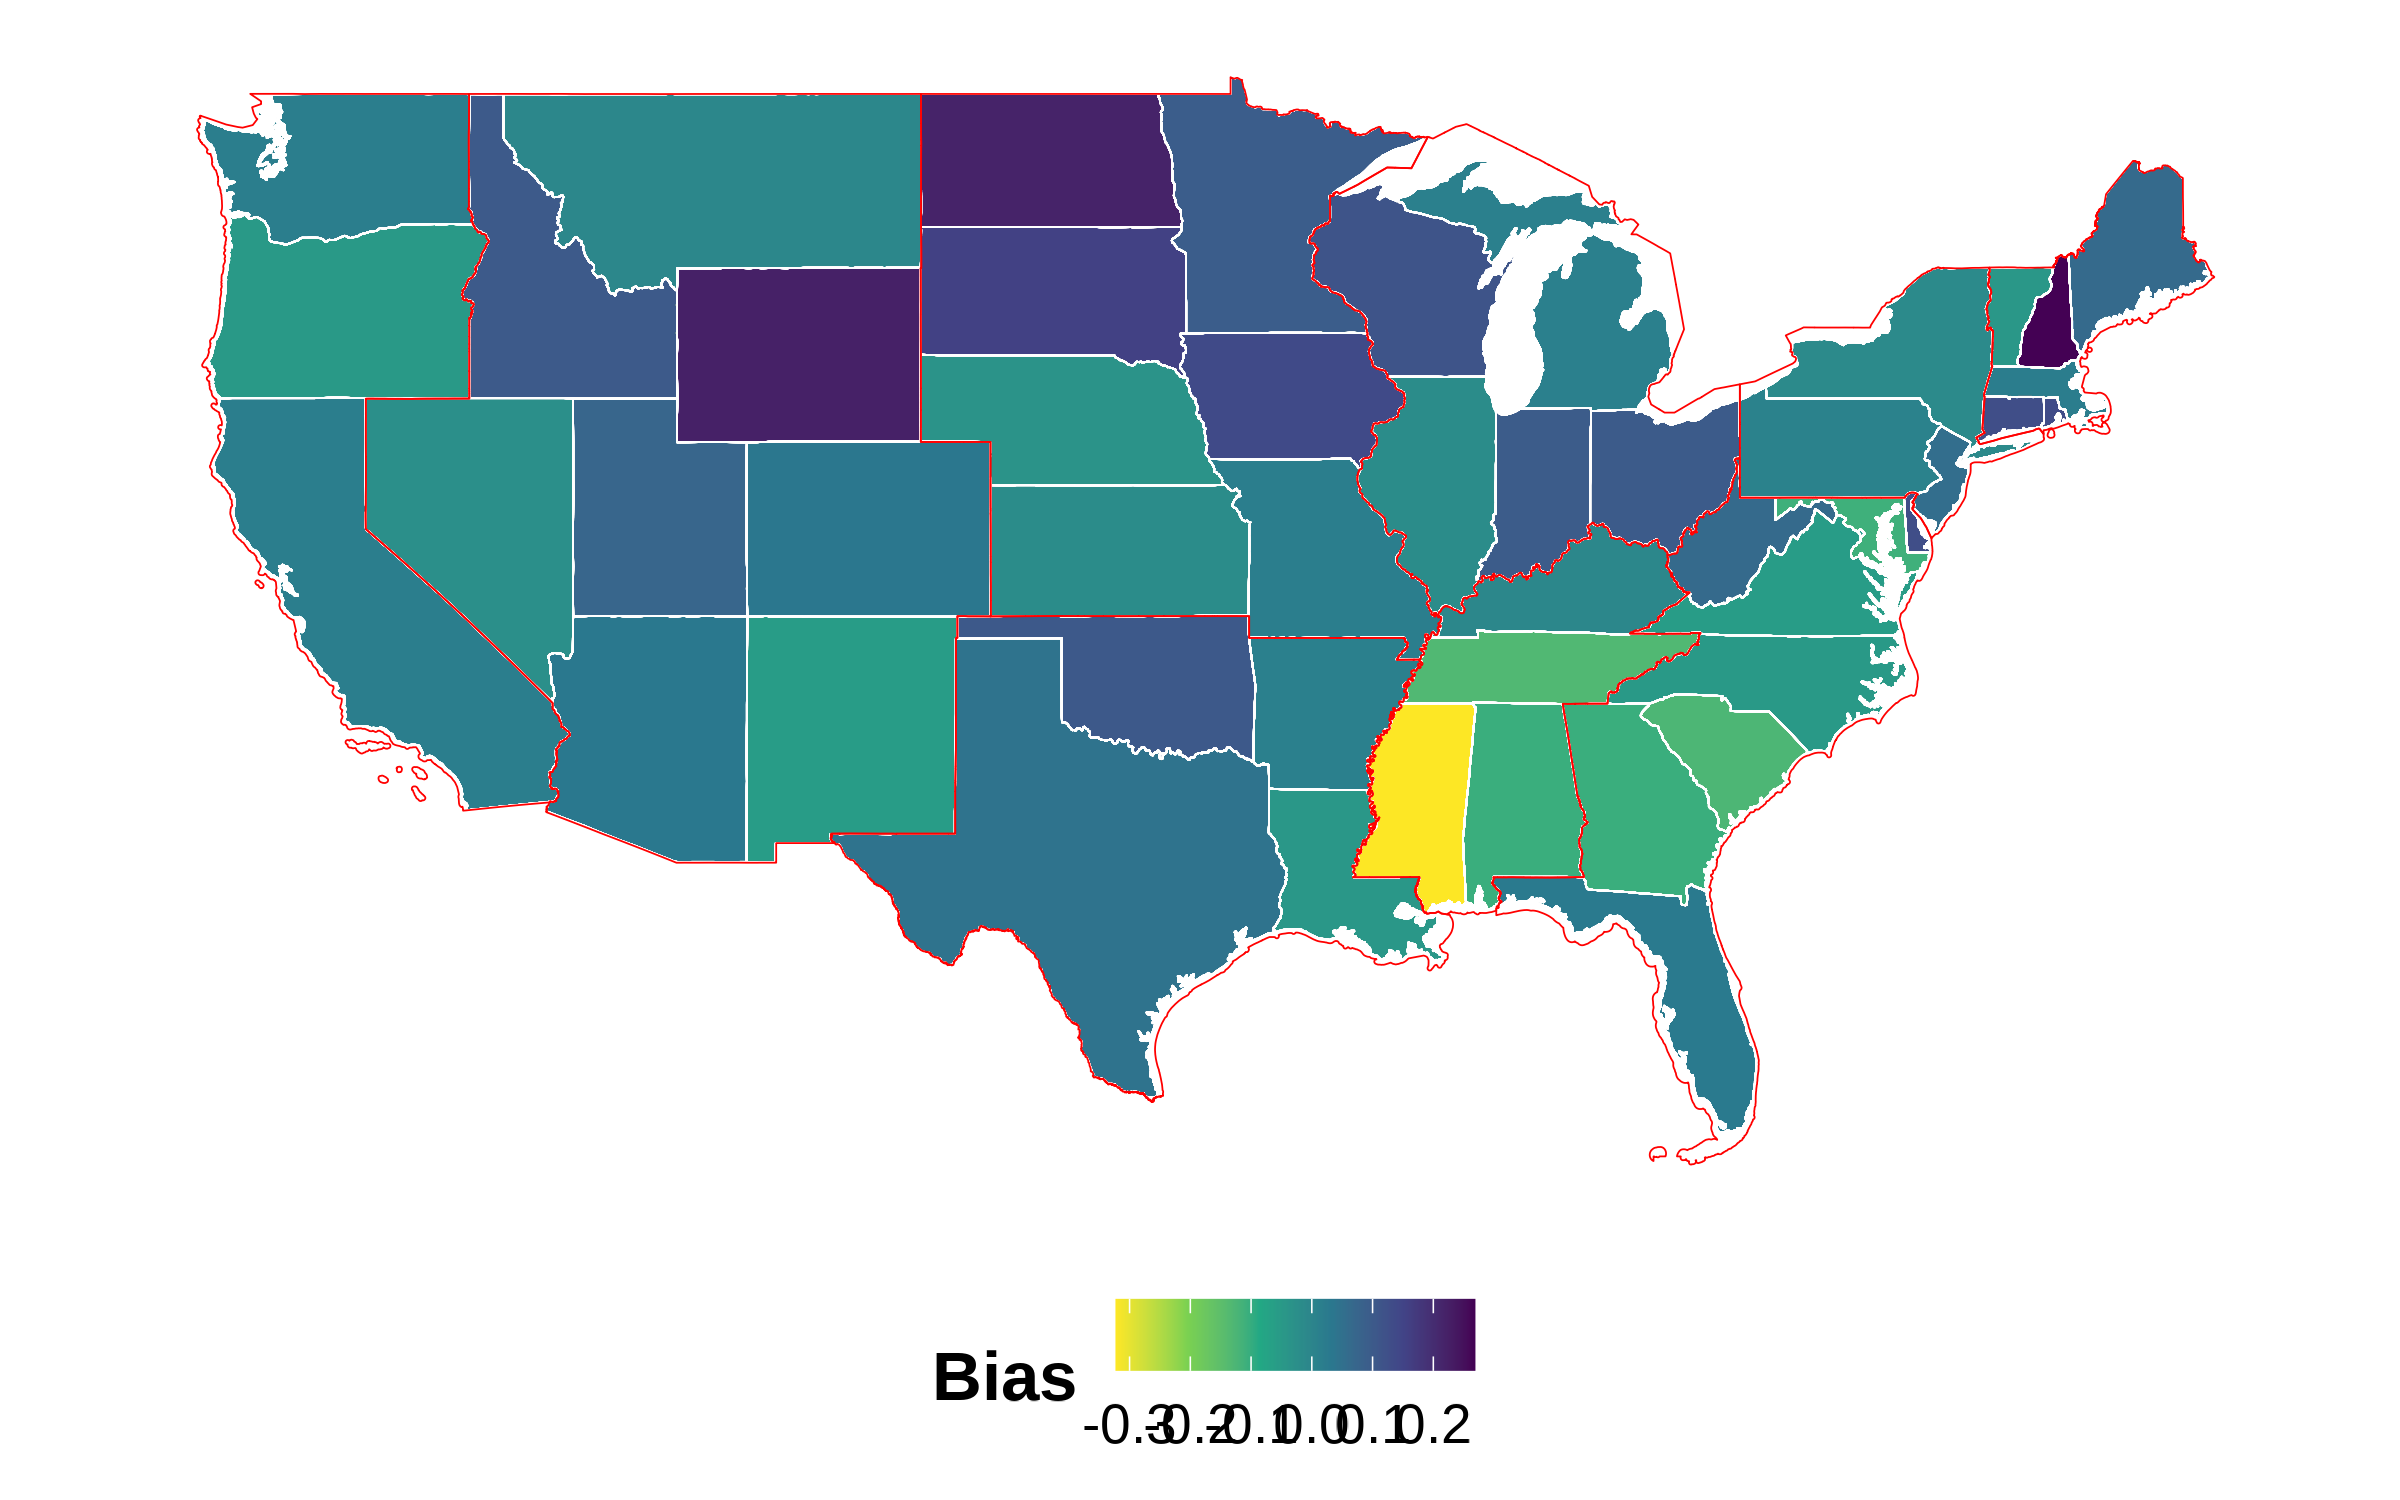
\includegraphics[width=\linewidth]{figure/2014skinmap.png} 
\label{fig:skiniat-map-2014}
\end{subfigure}
\hfill%
% seventh
\begin{subfigure}{.3\textwidth}
\caption{State-level Bias in 2016}
\centering
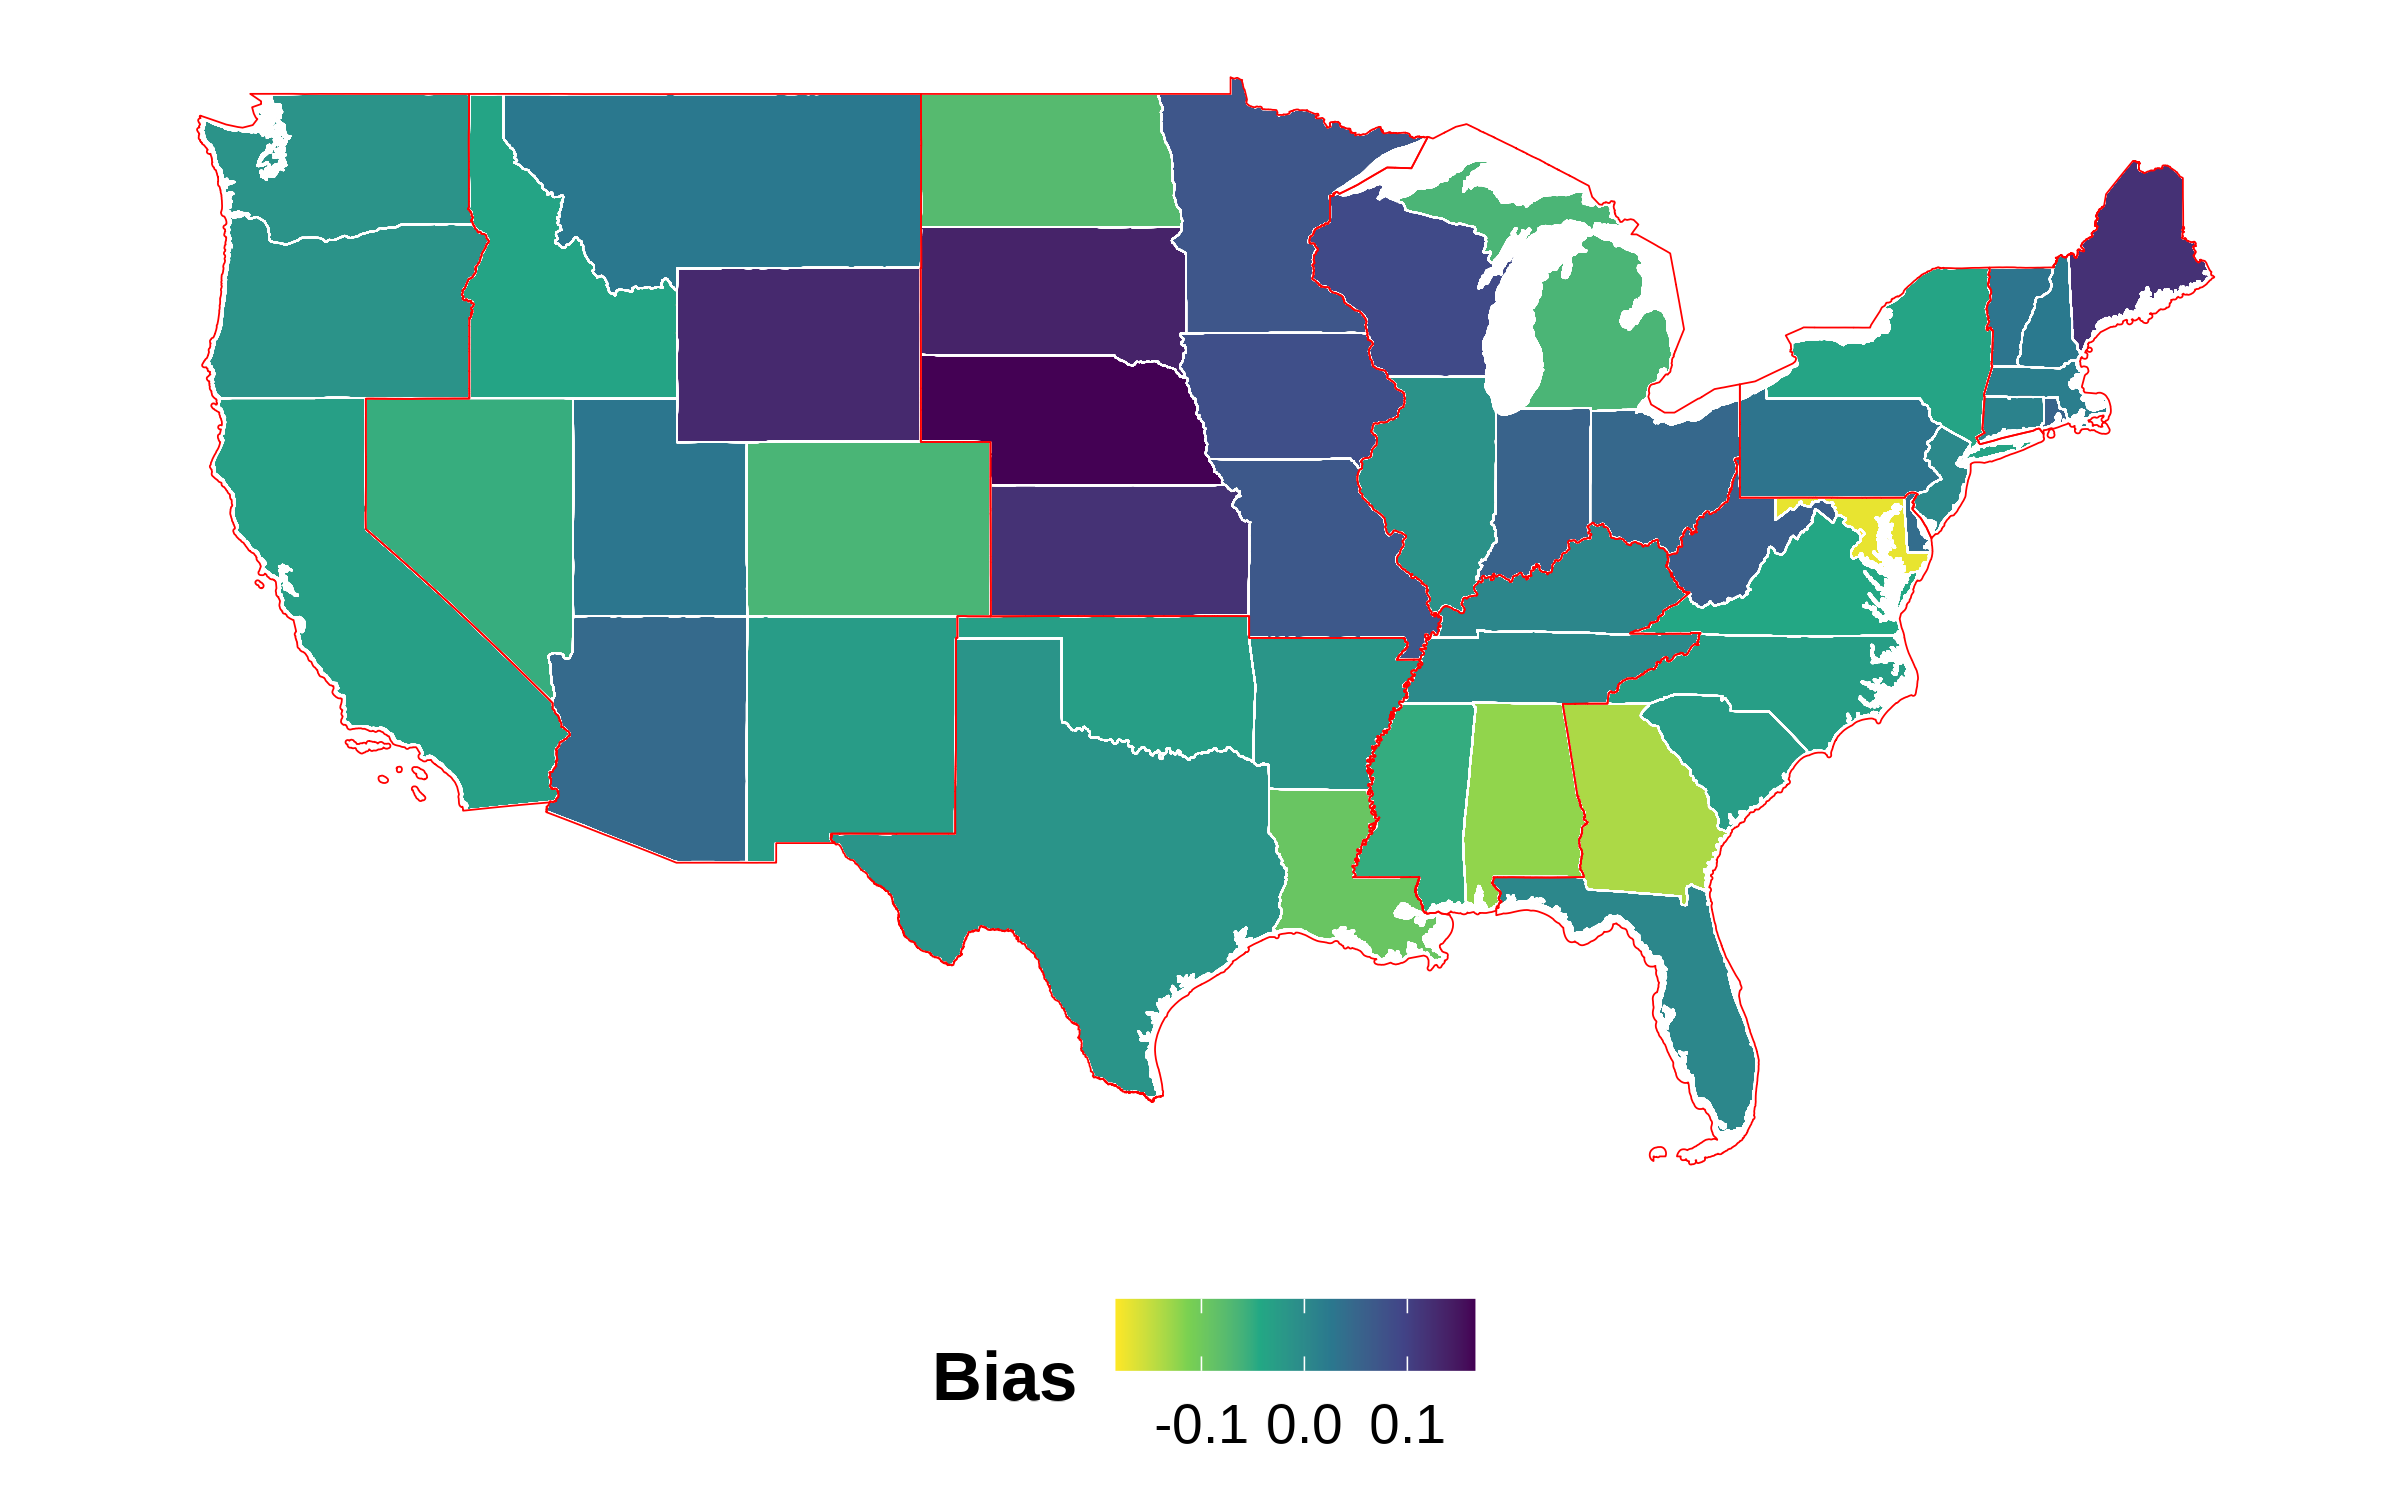
\includegraphics[width=\linewidth]{figure/2016skinmap.png} 
\label{fig:skiniat-map-2016}
\end{subfigure}
\hfill%
% eigth
\begin{subfigure}{.3\textwidth}
\hspace{1cm}
\caption{State-level Bias in 2018}
\centering
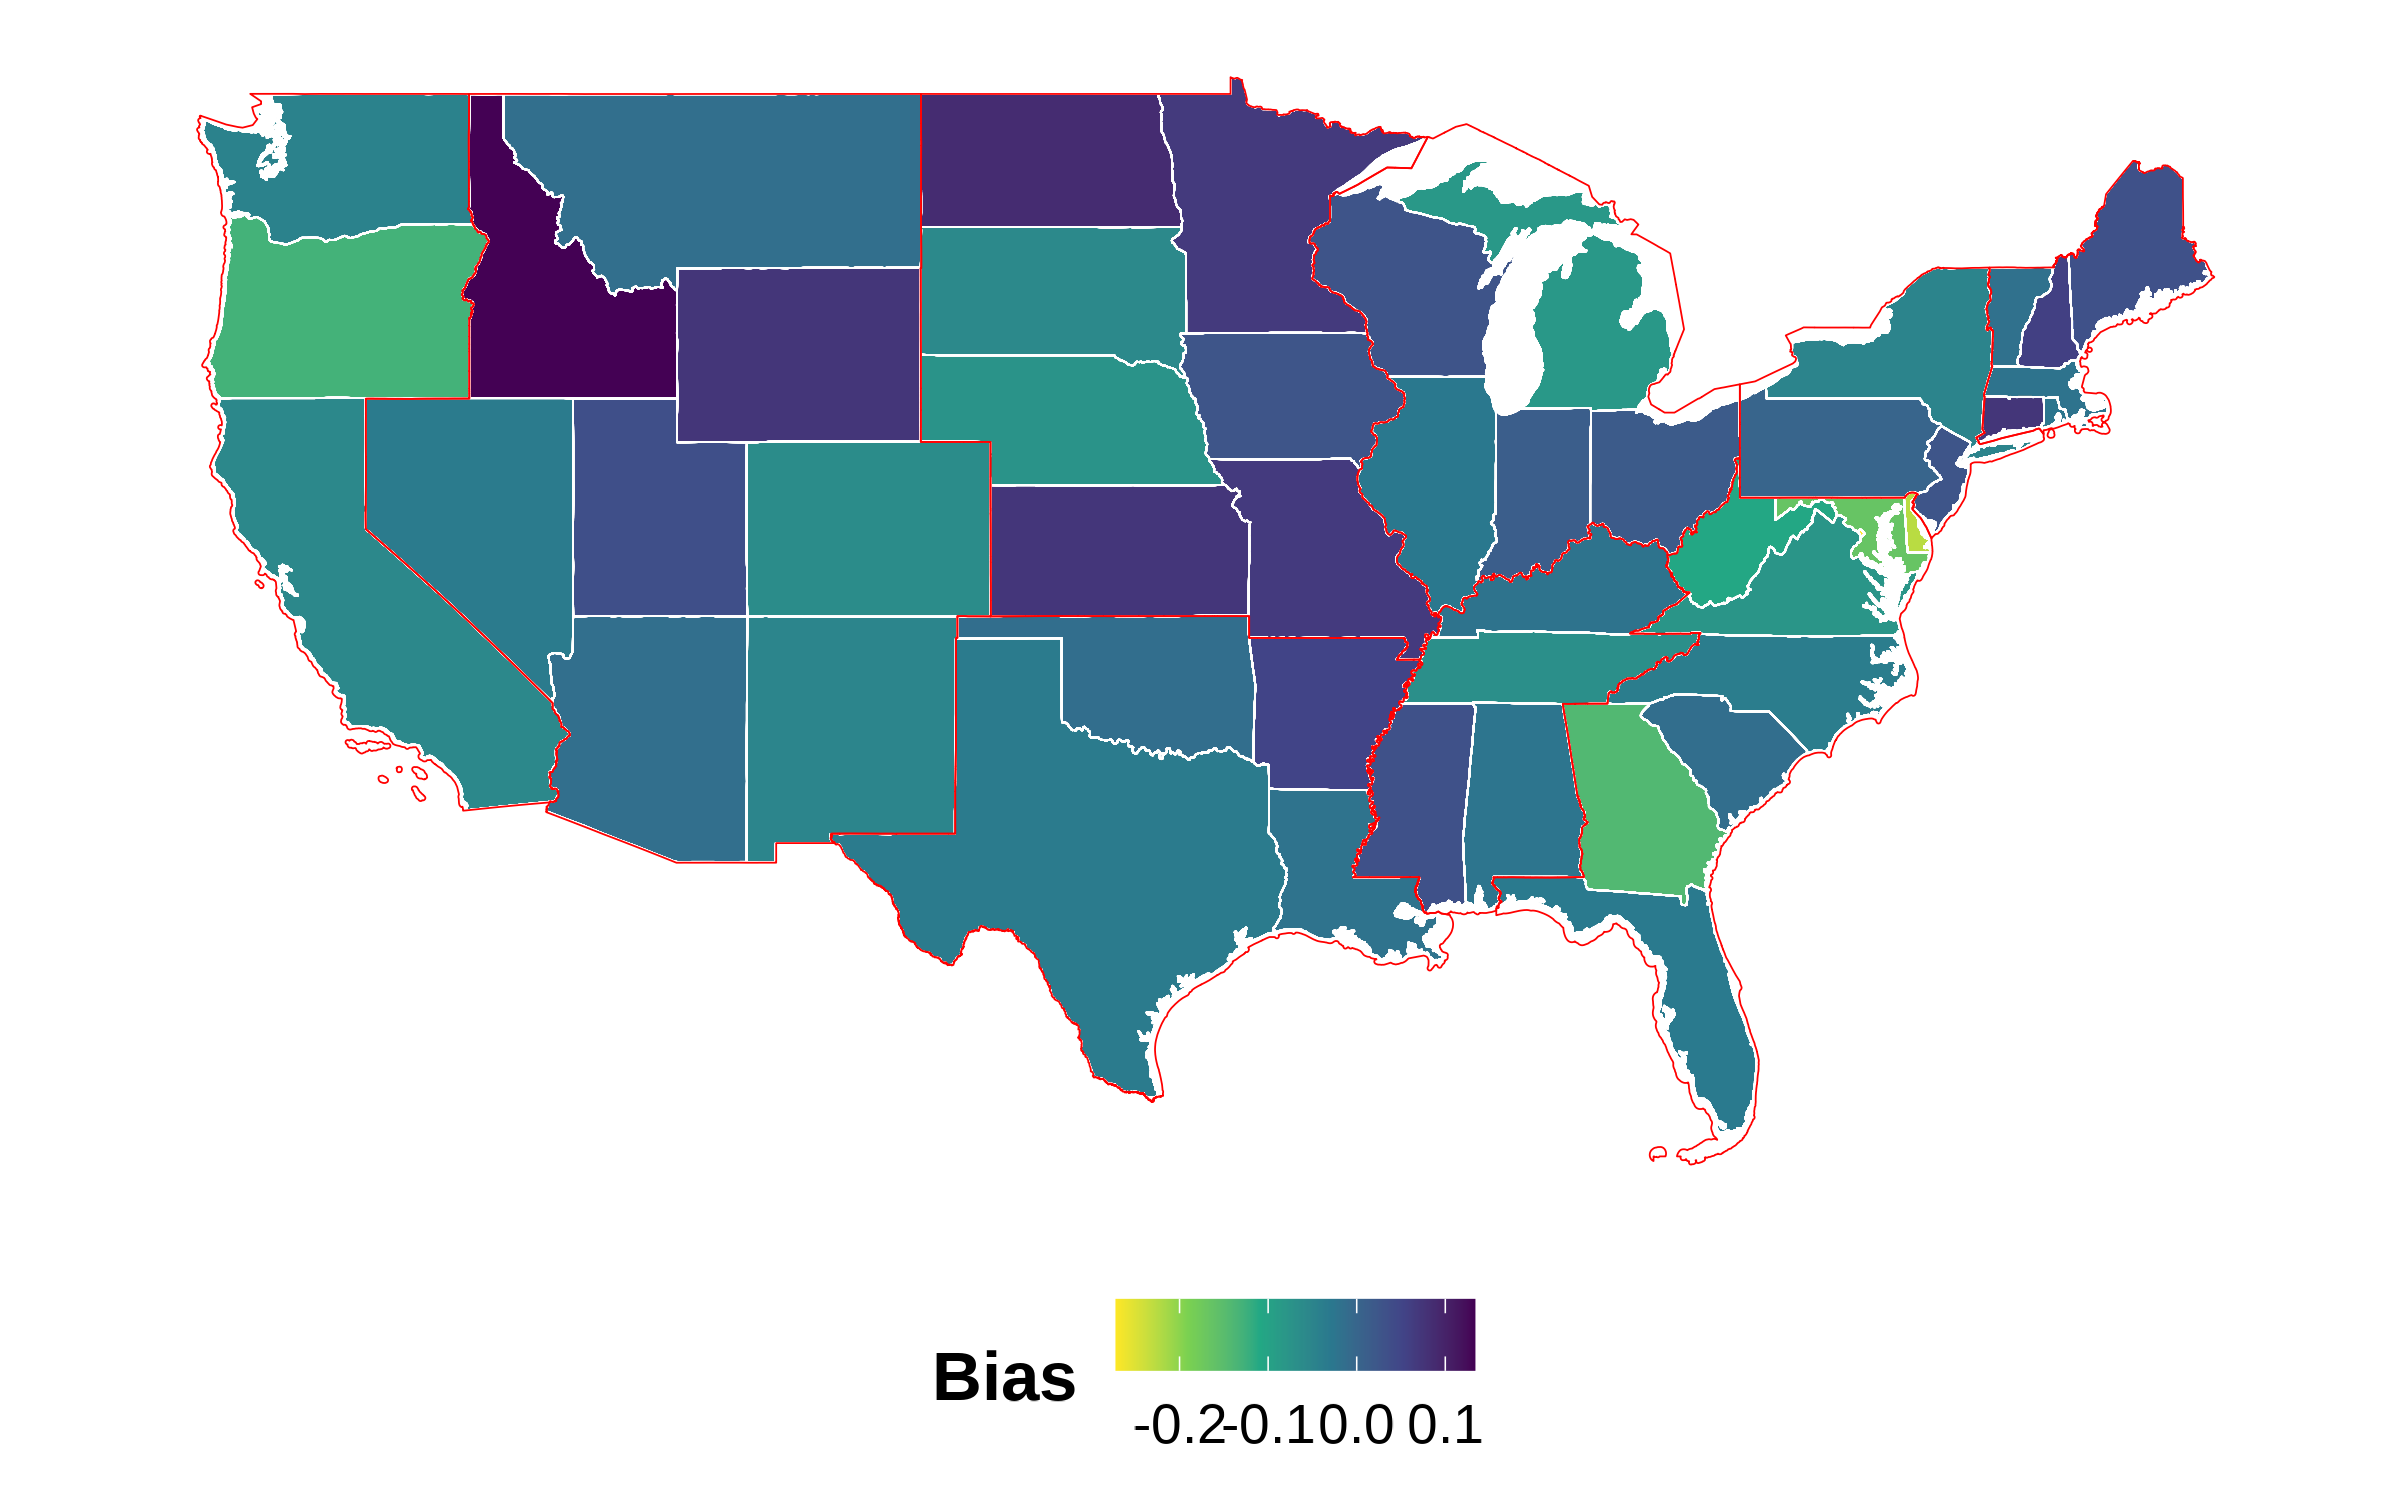
\includegraphics[width=\linewidth]{figure/2018skinmap.png} 
\label{fig:skiniat-map-2018}
\hfill%
\end{subfigure}
\flushleft\footnotesize{\note{In this figure, I show the state-level implicit bias in different years in the sample. Each panel presents state-level bias during a certain year. The boundaries in red represent the different Census divisions in the United States. Notice how there is a variation across states with-in a region.}}
\end{figure}
\end{center}



\newpage
\pagebreak

\begin{center}
\begin{figure}[H]
\caption{Maps of State-level Implicit Association Test Bias 2004-2021 Measure with Census Division Regional Boundaries}
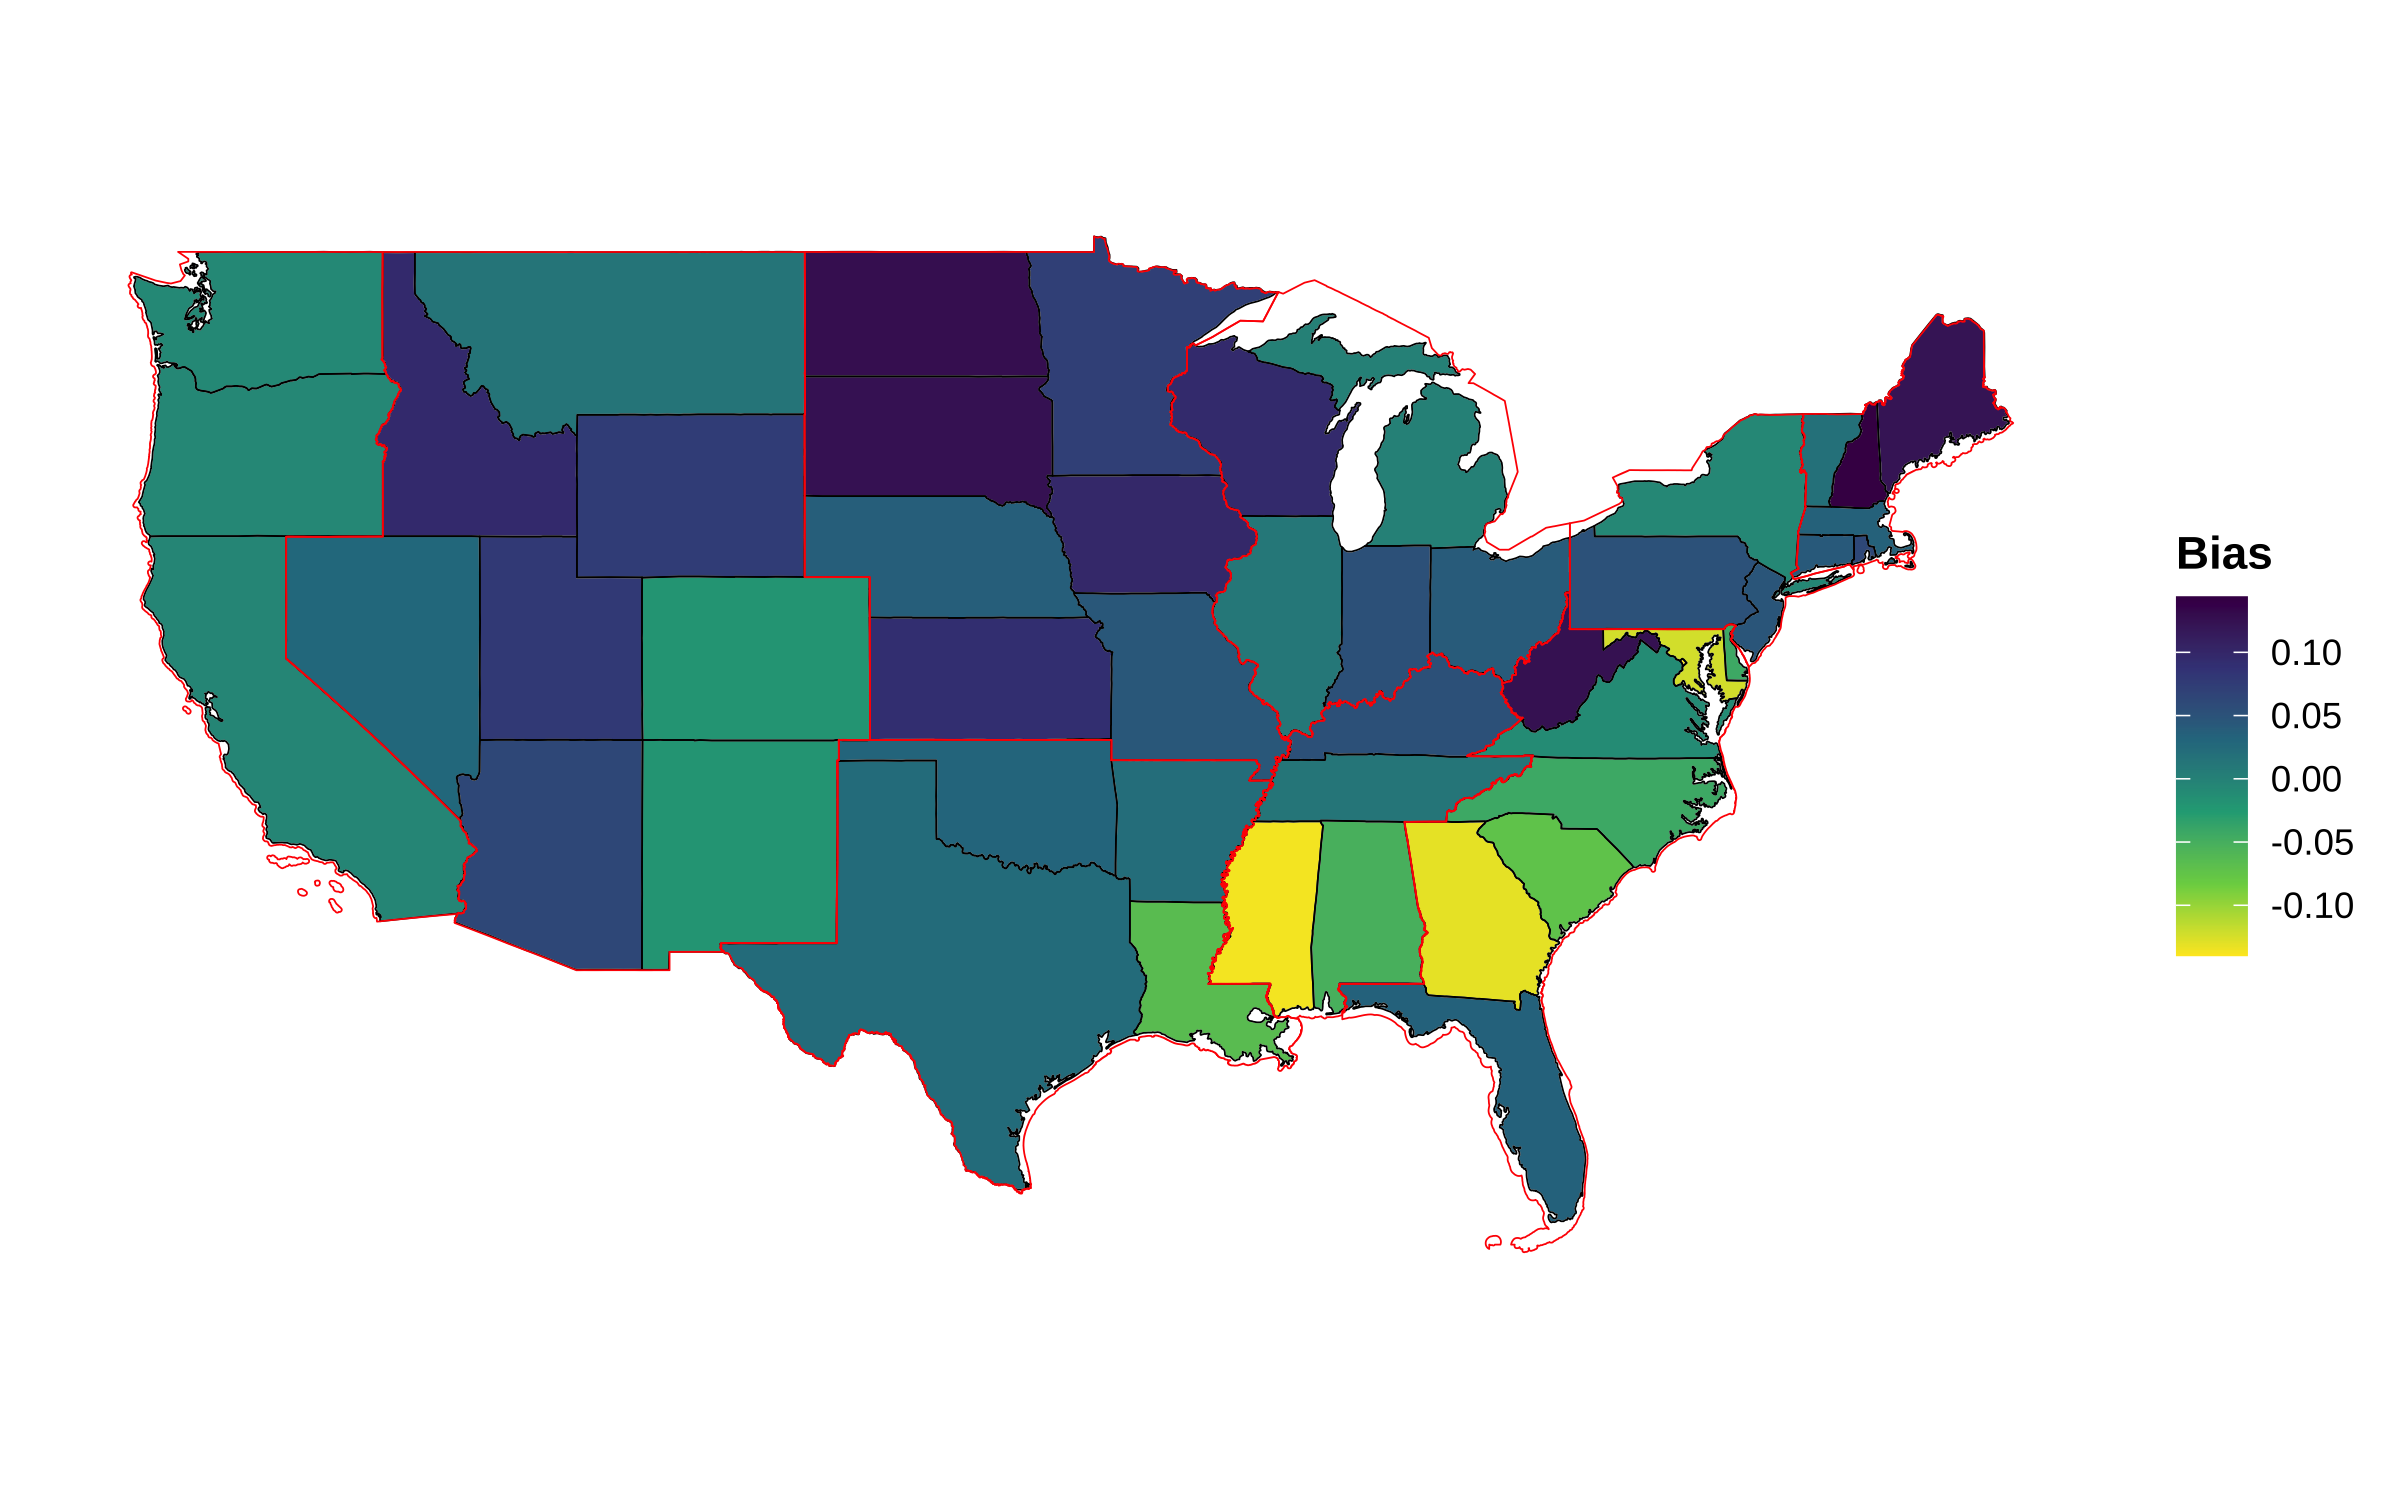
\includegraphics[width=\textwidth]{figure/skinmap_all.png} 
\label{fig:iat-map-all}
\flushleft\footnotesize{\note{In this figure, I show the state-level implicit bias in the sample of IAT tests from 2004 to 2021. The boundaries in red represent the different Census divisions in the United States. Notice how there is a variation across states with-in a region.}}
\end{figure}
\end{center}

\subsubsection{Measuring Prejudice}

The implicit association test measures how people associate concepts---for example, Black and dark-skinned people---and evaluations---good, bad. Respondents are asked to quickly match words into categories shown on a screen. I provide a few examples of what a test taker would see on a skin tone implicit association test by Harvard's Project Implicit in figure (\ref{fig:iatexamples}). 

% Therefore, the innovation of such a test lies in the fact that it could measure the attitudes and beliefs of people that they would be unwilling to report on a survey. For example, a person could believe that Black and White people are equally as likely to be good samaritans. However, their automatic association could show that Black people are associated with violence.

I use skin tone implicit association test data to construct a state-level prejudice \citep{greenwaldMeasuringIndividualDifferences1998}. This measure has been used in the social sciences, especially in psychology. Previous work has shown that IAT test scores are hard to manipulate \citep{egloffPredictiveValidityImplicit2002} and are correlated to economic outcomes \citep{chettyRaceEconomicOpportunity2020,gloverDiscriminationSelfFulfillingProphecy2017}, voting behavior \citep{friesePredictingVotingBehavior2007}, and health \citep{leitnerRacialBiasAssociated2016}. Moreover, \citet{bursztynImmigrantNextDoor2022} show that exposure to Arab and Muslim immigrants is predictive of lower IAT scores. I offer a graphical representation of the bias measure over time in the most and least biased places in (\ref{fig:skiniat}). A lower score implies less light-skin bias, whereas a higher score implies more discrimination against dark-skinned people. One-half of a standard deviation increase in bias is equivalent to the moving from Washington DC to North Dakota in 2012. I also show the state-level average bias over time in the maps in figure (\ref{fig:skiniat-maps}) and the overall average from 2004 to 2021 in figure (\ref{fig:iat-map-all}).

Participating in the IAT, an online test, is voluntary. Therefore, the samples are not random and might suffer from selection bias in who decides to take the exam. However,  bias reflected by Implicit Association Test (IAT) scores has been used as a proxy for prejudiced attitudes in an area \citet{chettyRaceEconomicOpportunity2020}. I provide a summary statistics of the sample in table (\ref{tab:sumstat-iat}). The average age of an Implicit Association Test (IAT) test taker is 28 years. Of the test takers, 68\% are women, and 62\% are Whites or 56\% non-Hispanic Whites. The test takers are highly educated. I also present the demographics of the representative Current Population Survey (CPS) sample over the same period in table (\ref{tab:sumstat-iat}). The CPS and IAT samples are different demographically, with the IAT sample being more female, less White, and with higher levels of education.


\begin{table}[H]

\caption{Skin Tone Implicit Association Test (IAT) Scores and Current Population Survey (CPS) Samples \label{tab:sumstat-iat}}
\centering
\begin{threeparttable}
\begin{tabular}[t]{>{}lcc}
\toprule
\multicolumn{1}{c}{ } & \multicolumn{1}{c}{IAT} & \multicolumn{1}{c}{CPS} \\
\cmidrule(l{3pt}r{3pt}){2-2} \cmidrule(l{3pt}r{3pt}){3-3}
Characteristic & N = 1,519,309 & N = 29,981,618\\
\midrule
\textbf{Age} & \makecell[c]{28 \\ (11)} & \makecell[c]{38 \\ (23)}\\
\textbf{Female} & 0.68 & 0.51\\
\textbf{White} & 0.62 & 0.81\\
\textbf{Non-Hispanic White} & 0.56 & 0.68\\
\textbf{Hispanic} & 0.14 & 0.13\\
\textbf{Education Levels} &  & \\
\hspace{1em}Bachelor's degree & 0.17 & 0.14\\
\hspace{1em}High school dropout & 0.10 & 0.33\\
\hspace{1em}High school graduate & 0.09 & 0.23\\
\hspace{1em}Master's degree & 0.12 & 0.06\\
\hspace{1em}Other & 0.48 & 0.21\\
\hspace{1em}Professional degree & 0.05 & 0.02\\
\textbf{Bias} & \makecell[c]{0.30 \\ (0.42)} & \\
\bottomrule
\multicolumn{3}{l}{\rule{0pt}{1em}\textsuperscript{*} Mean (SD)}\\
\end{tabular}
\begin{tablenotes}
\item[a] Data source is the 2004-2021 Harvard's Project Implicit Association Test scores and 2004-2020 Current Population Survey (CPS).
\end{tablenotes}
\end{threeparttable}
\end{table}


\subsection{Empirical Strategy}\label{sec:empstrat}

\subsubsection{The Determinants of Hispanic Identity} % (fold)
\label{sub:the_determinants_of_hispanic_identity}

I first estimate if state-level bias is correlated with self-reported Hispanic identity. Let $H^g$ be the self-reported Hispanic identity variable for a person from the $g^{th}$ generation, where $g \in \{1,2,3\}$, and $X$ be a vector of controls. I estimate different specifications for each generation $g$. The regression I will estimate is as follows:

\begin{align}
H_{ist}^g &= \beta_1^g Bias_{st} +\beta_2^g DadCollegeGrad_{ist}+\beta_3^g MomCollegeGrad_{ist}
           + \beta_4^g Woman_{ist} \nonumber\\
           &+ X_{ist}^g\pi + \gamma_{rt} 
           + \varepsilon_{ist}; 
           \text{where } g \in \{1,2,3\} \label{eq:identity_reg_bias}
\end{align}

Where $H^g_{ist}$ is the self-reported identity of person $i$ (whether the answer to ``Are you of Hispanic or Latino origin?'' was yes or no) that lives in state $s$ and was interviewed in year $t$, $Bias_{st}$ is the average bias in state $s$ at year $t$, $DadCollegeGrad_{ist}$ and $MomCollegeGrad_{ist}$ are indicator variables equal to 1 if the parents of person $i$ are college graduates and zero otherwise, and $Woman_{ist}$ is dummy variable that is equal to one if person $i$ is a woman. $X_{ist}^g$ is a vector of controls. Additionally, $\gamma_{rt}$ is region-time fixed effects that controls for region $\times$ year specific shocks. The region $\times$ year also controls for systematic differences between regions in the overall Hispanic population, or bias toward Hispanics, even if they vary over time.

The coefficient of interest in equation (\ref{eq:identity_reg_bias}), $\beta_1^g$, captures the relationship between state-level bias and self-reported Hispanic identity.  If $\beta_1^g > 0$, then individuals living in a state with higher bias would be more likely to self-report Hispanic identity. The coefficient $\beta_1^g$ captures the with-in region and across state variation in bias which could be seen in figures (\ref{fig:iat-map-all}), (\ref{fig:skiniat}), and (\ref{fig:hispanic-twostates}). In other words, I am estimating the relationship between bias and self-reported Hispanic identity by comparing states with-in a region to each other.

It could be the case that the desire to self-identify as Hispanic differs depending on the particular type of parents or grandparents. Consequently, I will further explore the relationship between bias and self-reported Hispanic identity by estimating the same equation by parents' and grandparents' types. I present another specification where I estimate the heterogeneous effect of bias on the different kinds of second- and third-generation immigrants by type of parents and grandparents, equation (\ref{eq:identity_reg_bias}). For example, I could estimate a regression on a sample of second-generation immigrants by parental type, where parental types depend on parental place of birth. I first estimate a model on a sample of second-generation immigrants by parents' types, then on third-generation immigrants by grandparents' types: 

\begin{align}
H_{ist}^2 &= \beta_1^2 Bias_{st} + \sum_{n}\delta_n^2 I_{\{ParentType_{ist} = n\}}  \label{eq:identity_reg_bias_interaction_2} \\
&+\sum_{m} \alpha_m^2 Bias_{st} \times I_{\{ParentType_{ist} = m\}} \nonumber \\
&+ \beta_3^2 DadCollegeGrad_{ist} + \beta_4^2 MomCollegeGrad_{ist} \nonumber \\ 
&+ \beta_5^2 Woman_{ist} + X_{ist}^2\pi + \gamma_{rt} + \varepsilon_{ist} \nonumber
\end{align}

\begin{align}
H_{ist}^3 &= \beta_1^3 Bias_{st} + \sum_{n}\delta_n^3 I_{\{GrandParentType_{ist} = n\}}  \label{eq:identity_reg_bias_interaction_3} \\
&+\sum_{m} \alpha_m^3  Bias_{st} \times I_{\{GrandParentType_{ist} = m\}} \nonumber \\
&+ \beta_3^2 DadCollegeGrad_{ist} + \beta_4^2 MomCollegeGrad_{ist} \nonumber \\ 
&+ \beta_5^2 Woman_{ist} + X_{ist}^2\pi + \gamma_{rt} + \varepsilon_{ist} \nonumber
\end{align}

Where $H_{ist}^2$ and $H_{ist}^3$ are the self-reported identity of second and third-generation person $i$ that lives in state $s$ at time $t$. Regressions (\ref{eq:identity_reg_bias_interaction_2}) and (\ref{eq:identity_reg_bias_interaction_3}) include the state-year average bias, indicator variables $I_{\{ParentType_{ist} = n\}}$ and $I_{\{GrandParentType_{ist} = n\}}$, and the interaction between the bias and parental and grandparent type. The variable ~$I_{\{ParentType_{ist} = n\}}$ ~includes three categories of parents: 1) father born in a Spanish Speaking country and mother born in a Spanish-speaking country, or Hispanic-Hispanic (HH) and I will use as the reference category, 2) father born in a Spanish Speaking country and mother born in the US, or Hispanic-White (HW), 3) father born in the US and mother born in a Spanish speaking country, or White-Hispanic (WH). Thus, indicator variable $I_{\{ParentType_{ist} = WH \}}$ is equal to one if the person $i$ has an objectively White father-Hispanic mother, and zero otherwise. The variable $I_{\{GrandParentType_{ist} = n\}}$ includes 15 possible combinations of the types of grandparents: 1) paternal grandfather born in a Spanish-speaking country, paternal grandmother born in a Spanish-speaking country, maternal grandfather born in a Spanish speaking country, and maternal grandmother born in a Spanish speaking country (HHHH) and I will use as the reference category, 2) paternal grandfather born in a Spanish speaking country, paternal grandmother born in a Spanish speaking country, maternal grandfather born in a Spanish speaking country, and maternal grandmother born in the US (HHHW), 3) paternal grandfather born in a Spanish speaking country, paternal grandmother born in a Spanish speaking country, maternal grandfather born in in the US, and maternal grandmother born in the US (HHWW), etc. 

The coefficients of interest in equation (\ref{eq:identity_reg_bias_interaction_2}), $\alpha_n^2$, capture the relationship between state-level bias and self-reported Hispanic identity by parents' type of second-generation immigrants. In other words, $\alpha_n^2$ estimates the difference in self-reported Hispanic identity between children of Hispanic-White (HW) and White-Hispanic (WH) and the reference group Hispanic-Hispanic (HH) and its relationship with bias. For example, if $\alpha_1^2$, the coefficient of the indicator variable $I_{\{ParentType_{ist} = White-Hispanic (WH)\}}$, is $\alpha_1^2 > 0$, then the difference between the child of an objectively White father and Hispanic mother (WH) and objectively Hispanic father and Hispanic mother (HH) is positively correlated with state-level bias. Consequently, an increase in bias is associated with higher self-reported Hispanic identity among objectively White father and Hispanic mother (WH) children compared to objectively Hispanic father and Hispanic mother (HH) children. 

Furthermore, the coefficients of interest in equation (\ref{eq:identity_reg_bias_interaction_3}), $\alpha_m^3$, captures the relationship between state-level bias and self-reported Hispanic identity by grandparents' type of third-generation immigrants. For example, if $\alpha_1^3$, the coefficient of the indicator ~variable \newline $I_{\{GrandParentType_{ist} = Hispanic-Hispanic-White-White (HHWW)\}}$, ~is ~$\alpha_1^3 > 0$. In this case, the difference between the child of objectively Hispanic-Hispanic-White-White grandparents (HHWW) and objectively Hispanic-Hispanic-Hispanic-Hispanic (HHHH) grandparents is positively correlated with state-level bias. Consequently, an increase in bias is correlated with higher self-reported Hispanic identity among objectively Hispanic-Hispanic-White-White (HHWW) children compared to objectively Hispanic-Hispanic-Hispanic-Hispanic (HHHH). 

\begin{center}
\begin{figure}[H]
\centering
\caption{Relationship Between Self-Reported Hispanic Identity and Bias: By Generation}
\label{plot01-regression-gen}
%First graph
\begin{subfigure}{.48\textwidth}
\caption{All Generations}
\centering
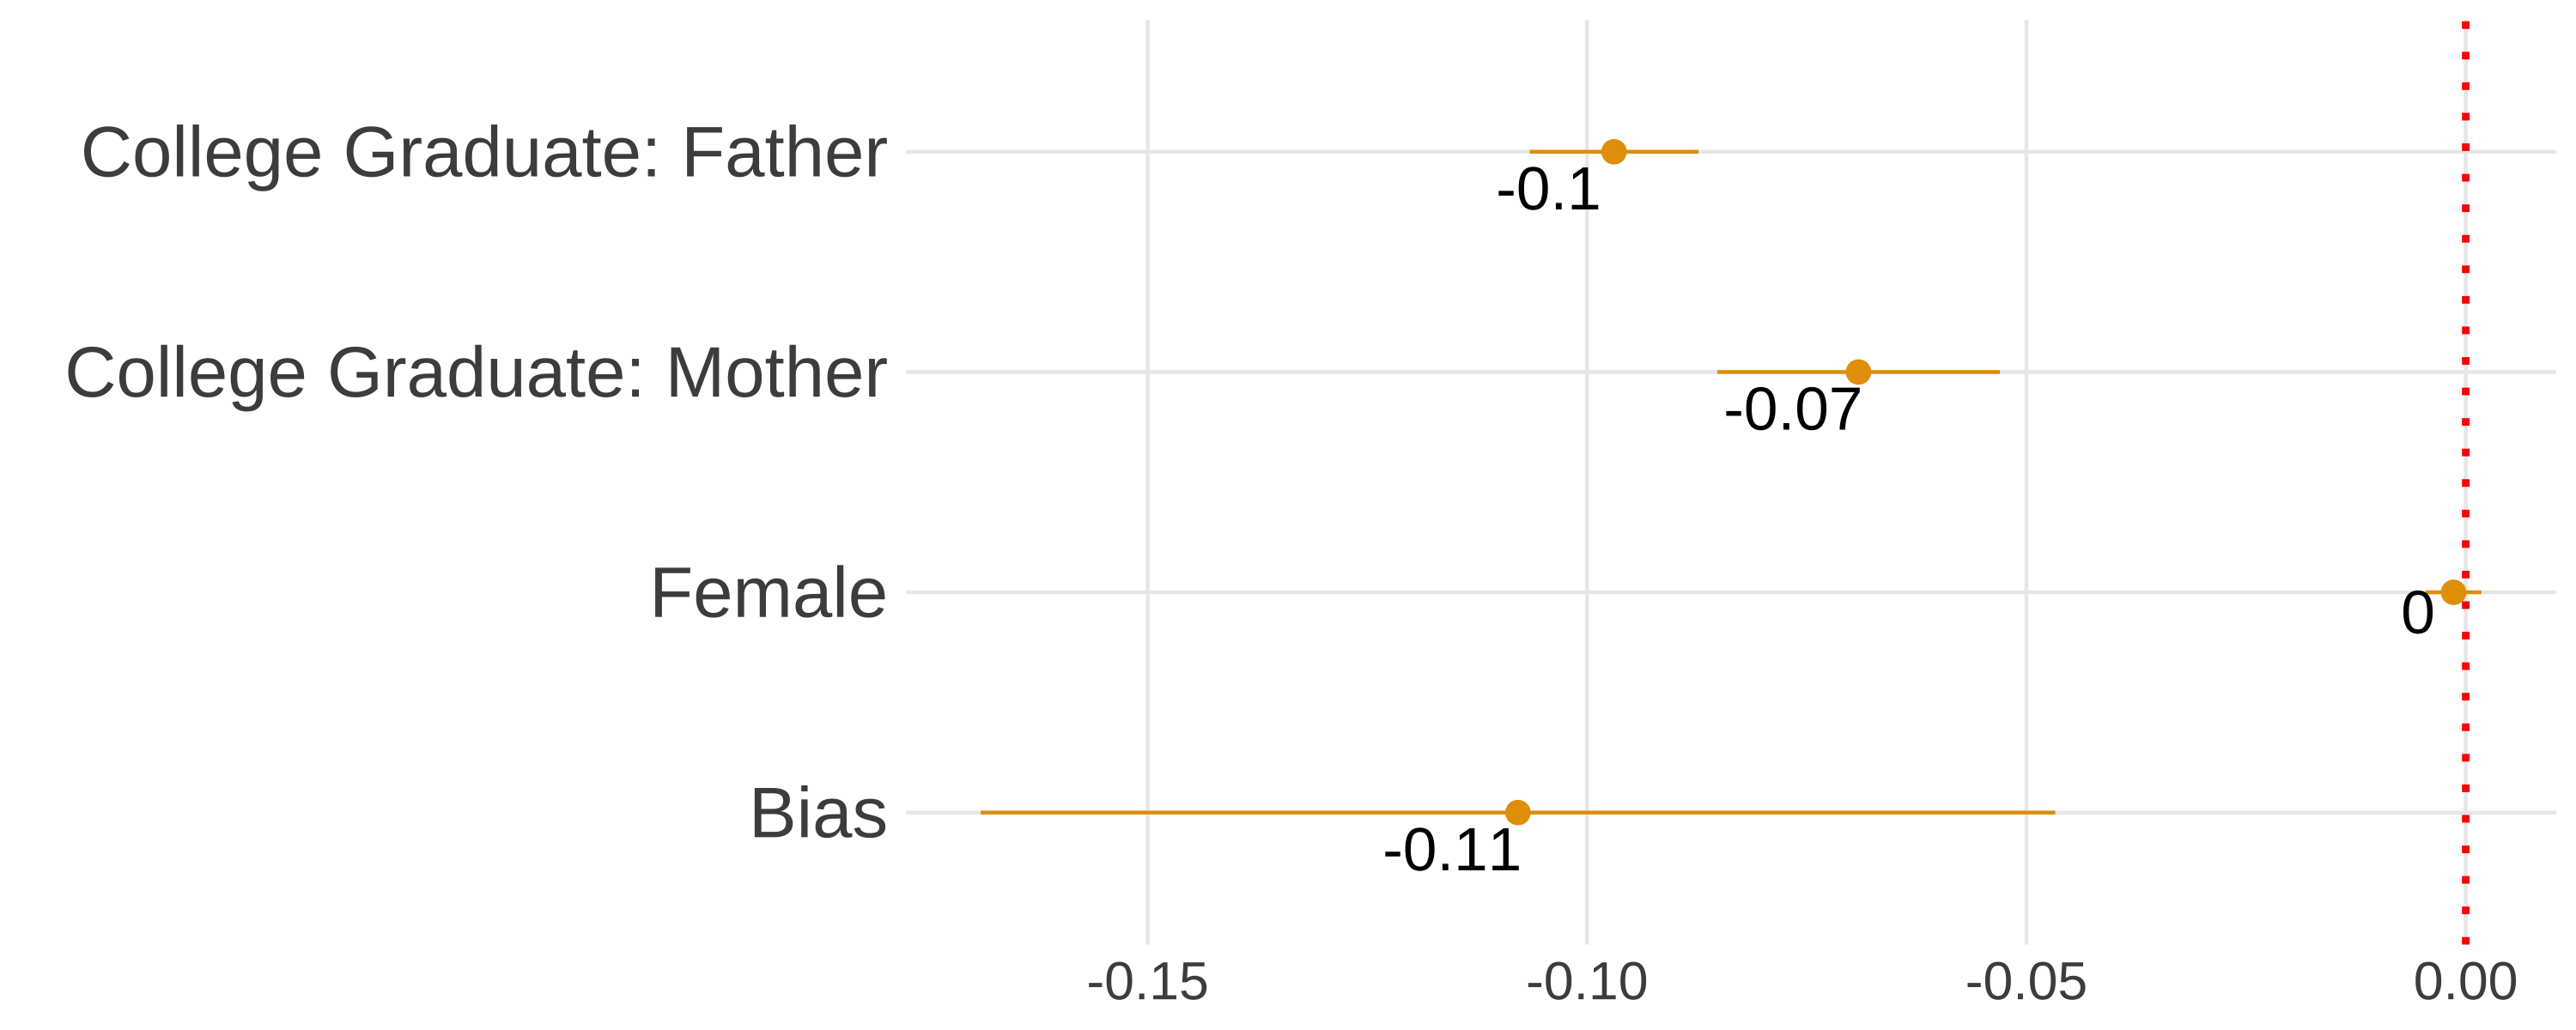
\includegraphics[width=.9\linewidth]{figure/skin-iat-regression-all-gens.png}
\end{subfigure}
\centering
%Second graph
\begin{subfigure}{.48\textwidth}
\caption{First-Generation}
\centering
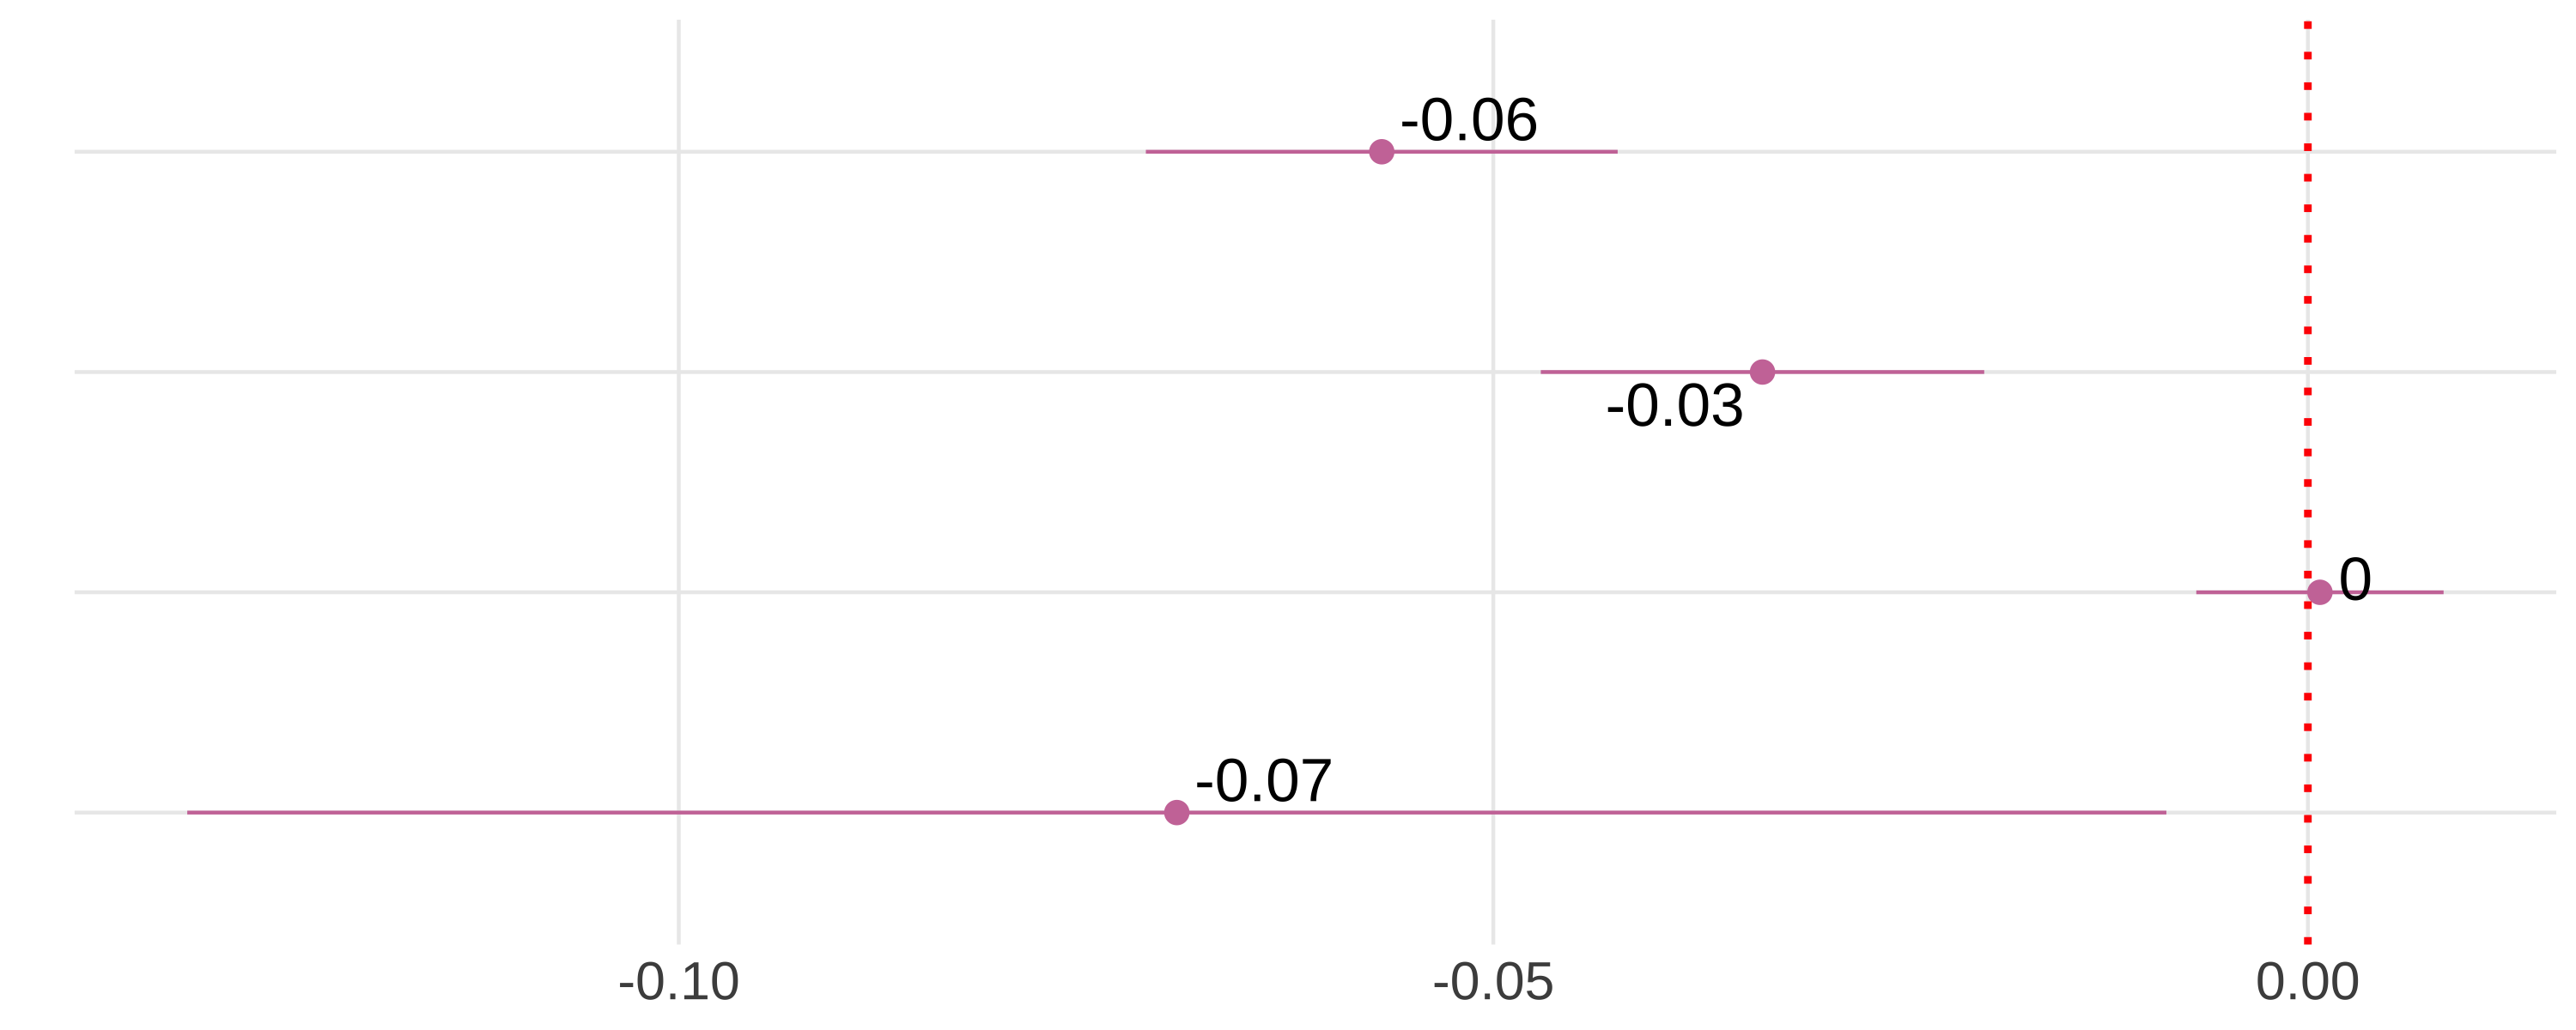
\includegraphics[width=.9\linewidth]{figure/skin-iat-regression-first-gen.png}
\end{subfigure}
%Third Graph
\begin{subfigure}{.48\textwidth}
\caption{Second-Generation}
\centering
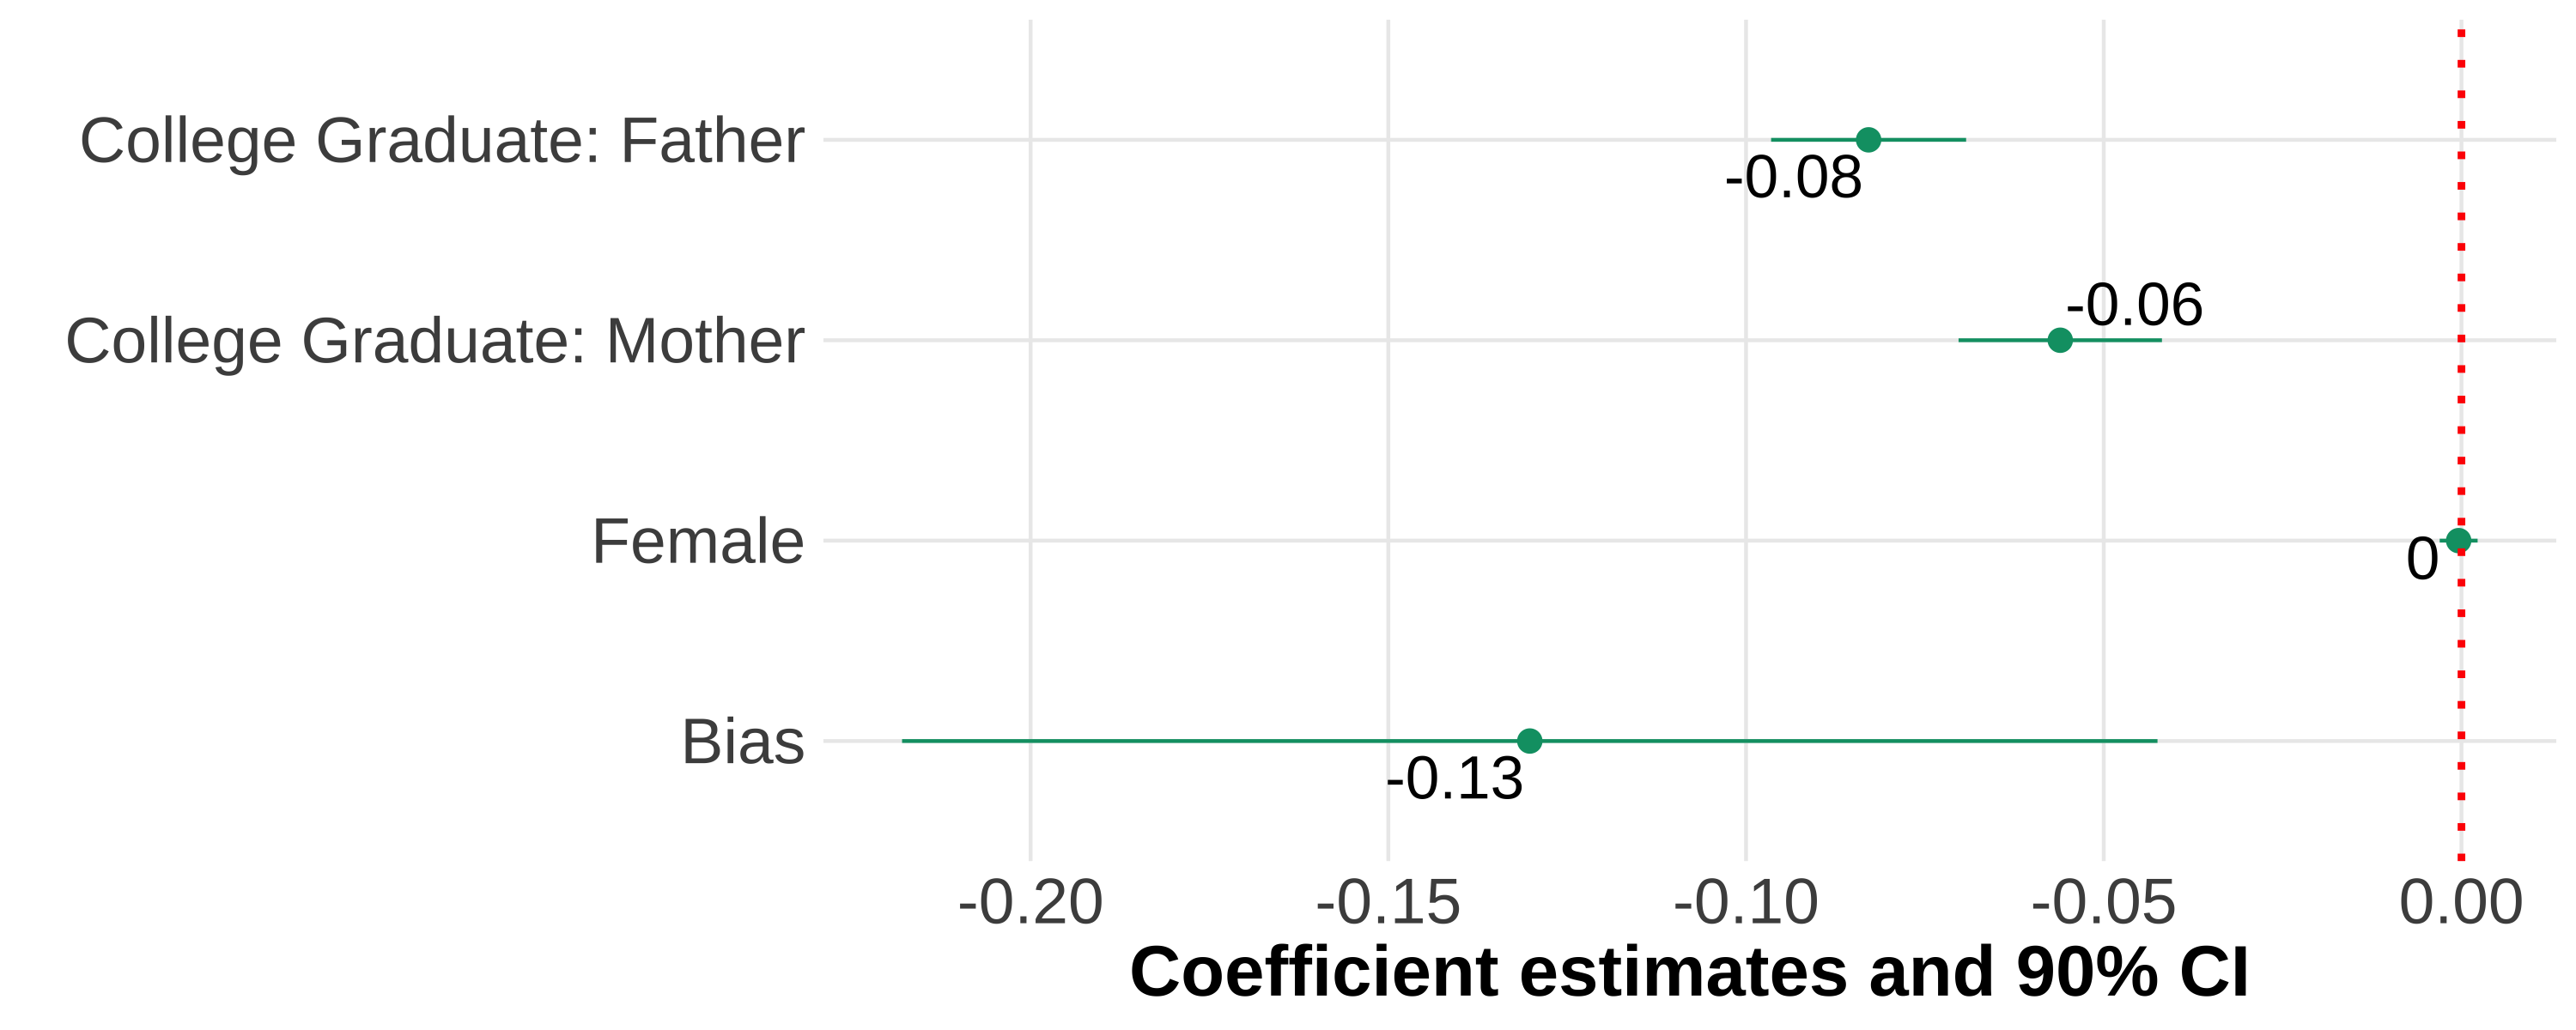
\includegraphics[width=.9\linewidth]{figure/skin-iat-regression-second-gen.png}
\end{subfigure}
%Fourth Graph
\begin{subfigure}{.48\textwidth}
\caption{Third-Generation}
\centering
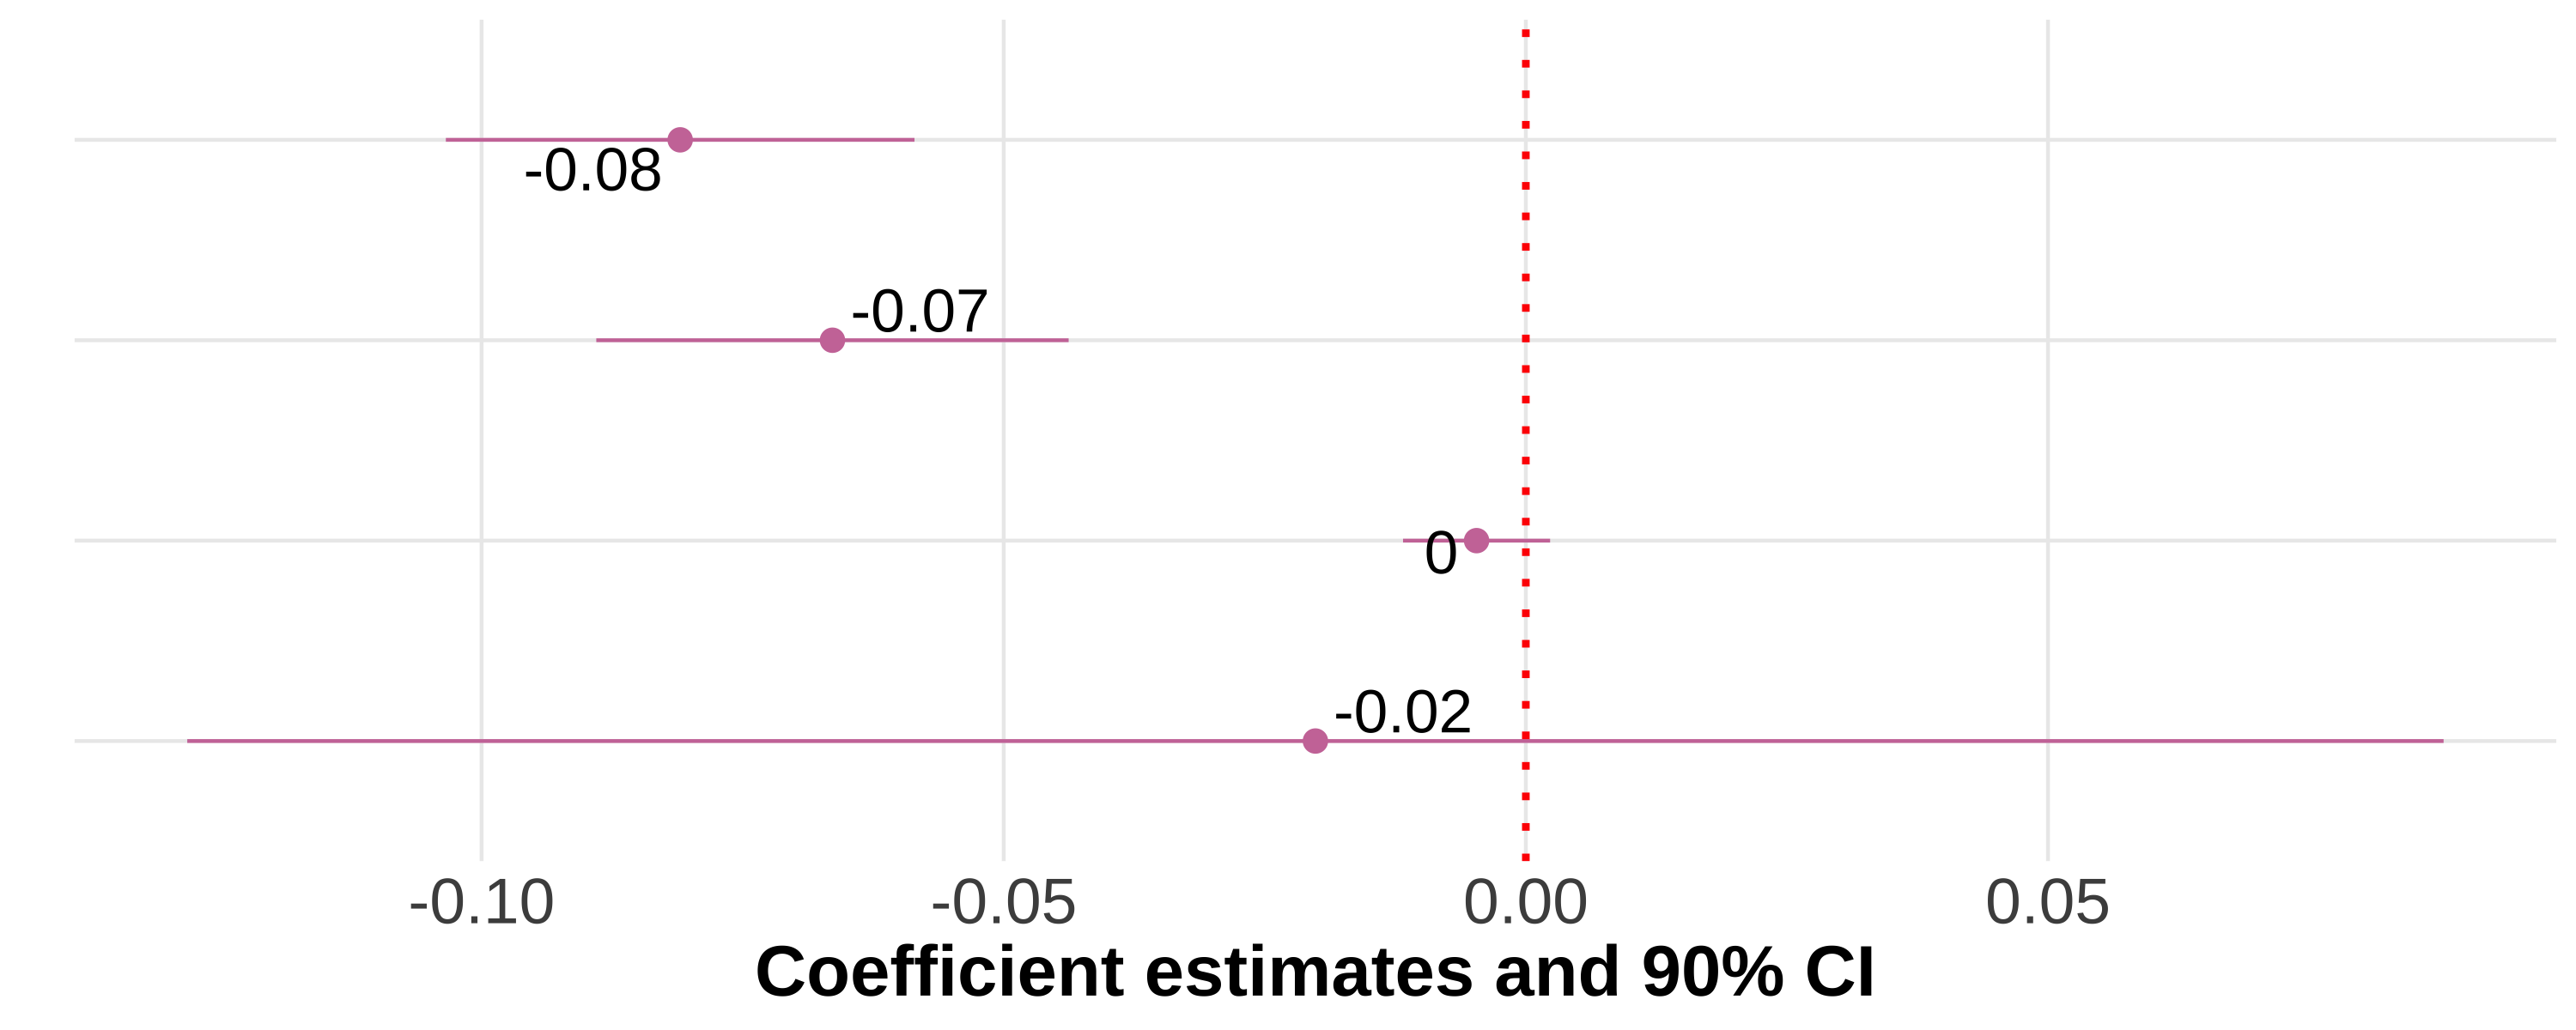
\includegraphics[width=.9\linewidth]{figure/skin-iat-regression-third-gen.png}
\end{subfigure}
\flushleft\footnotesize{\note{I show four panels of estimating equation (\ref{eq:identity_reg_bias}). I include region $\times$ year fixed effects with controls for sex, quartic age, and parental education. The dependent variable is self-reported Hispanic identity and the independent variable is state-level bias. Each panel is the results from the same regression but on different samples that are divided by generation. Standard errors are clustered on the state level. The samples include first-, second-, and third-generation Hispanic children ages 17 and below who live in intact families. First-generation Hispanic immigrants are children that were born in a Spanish-speaking county. Native-born second-generation Hispanic immigrants are children with at least one parent born in a Spanish-speaking country. Finally, native-born third-generation Hispanic immigrants are children with native-born parents and at least one grandparent born in a Spanish-speaking country.}}
\end{figure}
\end{center}

\begin{center}
\begin{figure}[H]
\centering
\caption{Relationship Between Self-Reported Hispanic Identity and Bias: By Parental Types}
\label{plot01-regression-byparent}
%First graph
\begin{subfigure}{.48\textwidth}
\caption{Second-Generation (All Parental Types)}
\centering
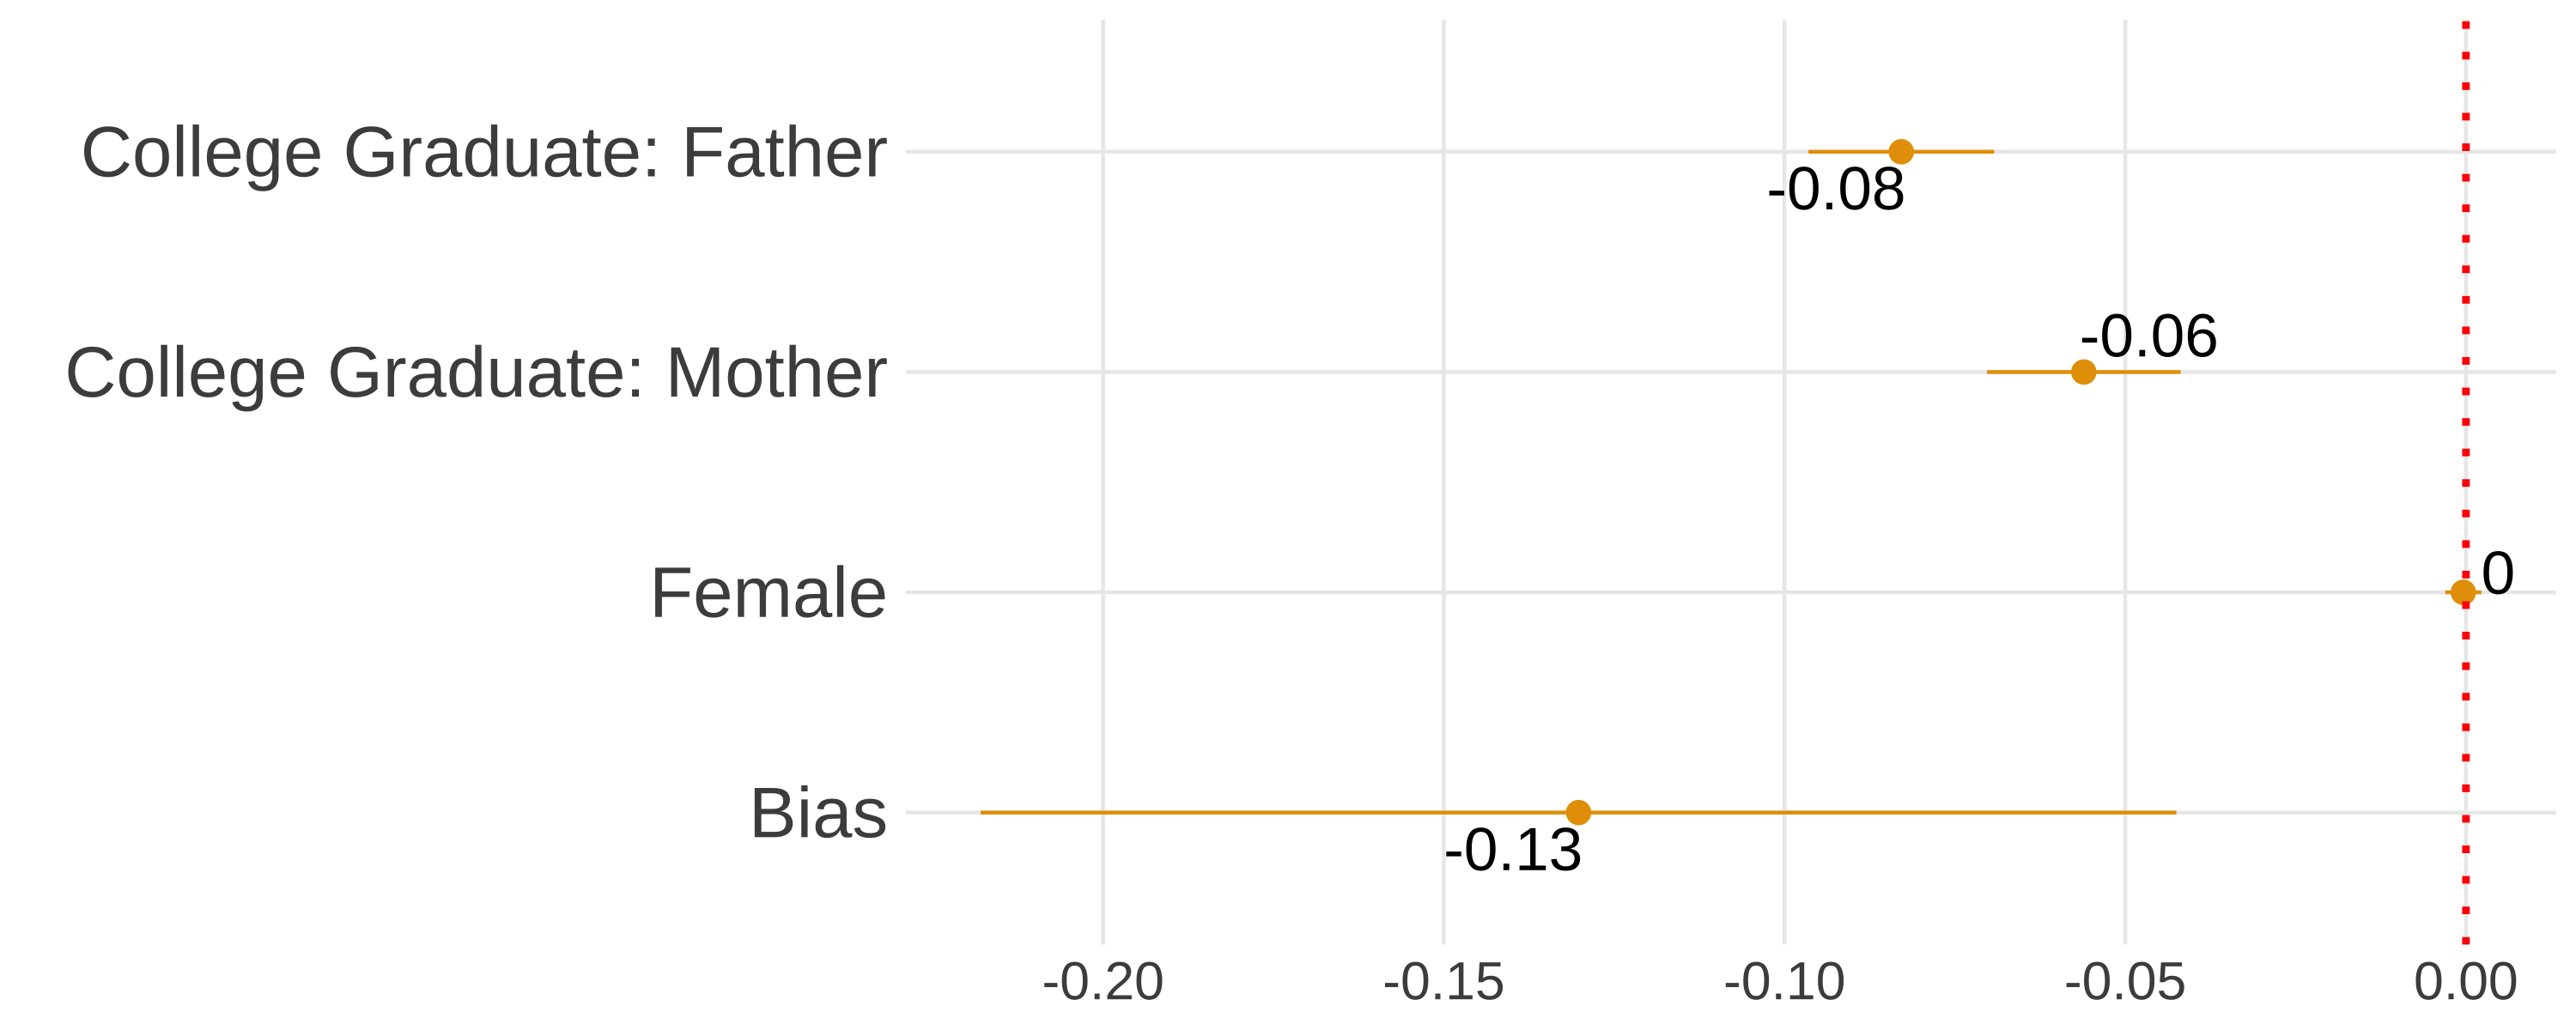
\includegraphics[width=.9\linewidth]{figure/by-parents-regs-all.png}
\end{subfigure}
\centering
%Second graph
\begin{subfigure}{.48\textwidth}
\caption{Hispanic Fathers-Hispanic Mothers}
\centering
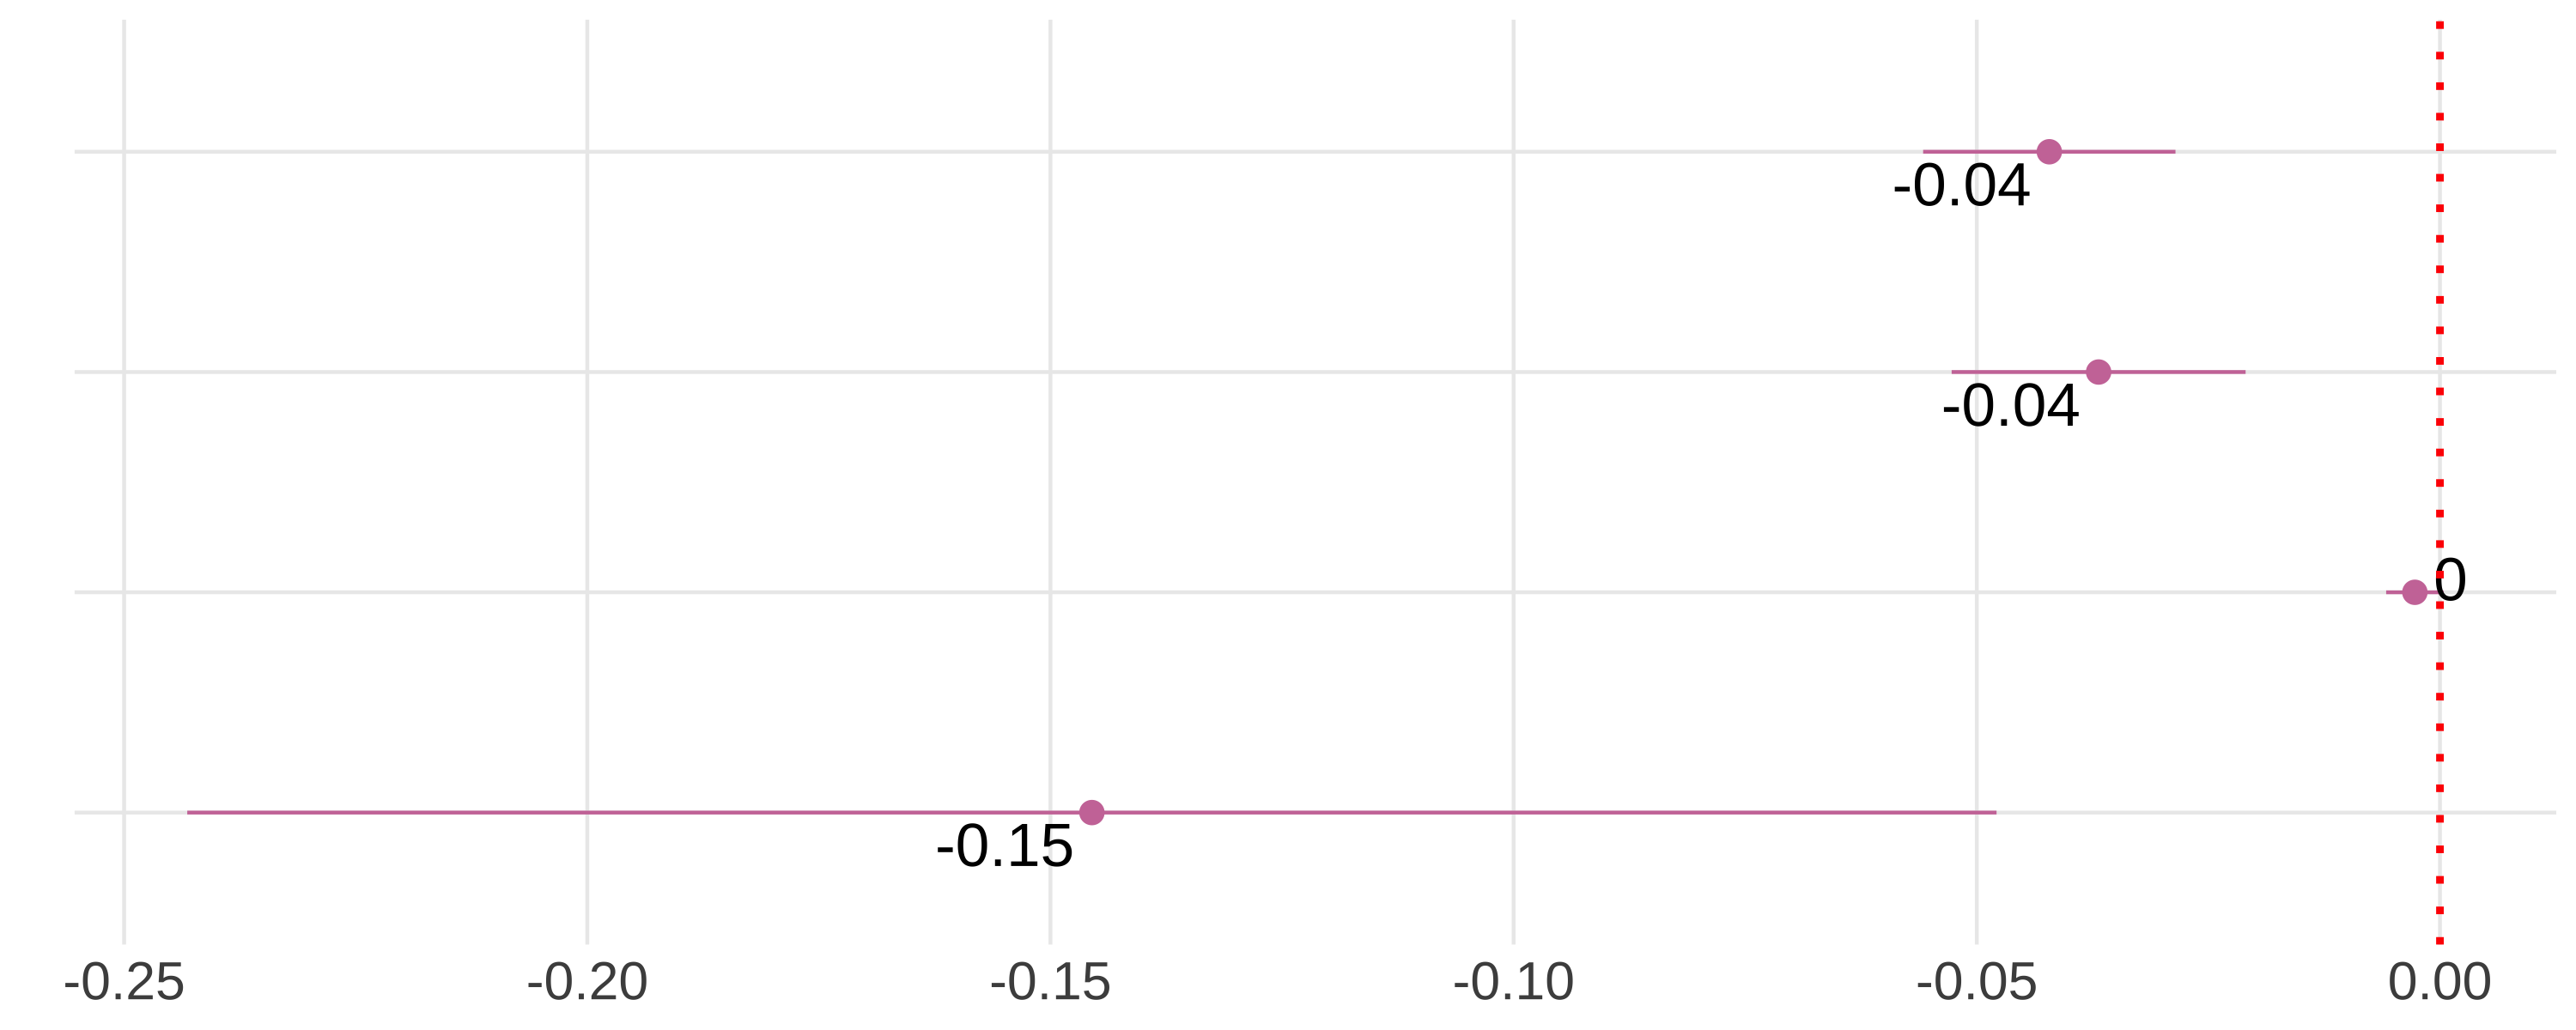
\includegraphics[width=.9\linewidth]{figure/by-parents-regs-hh.png}
\end{subfigure}
%Third Graph
\begin{subfigure}{.48\textwidth}
\caption{Hispanic Fathers-White Mothers}
\centering
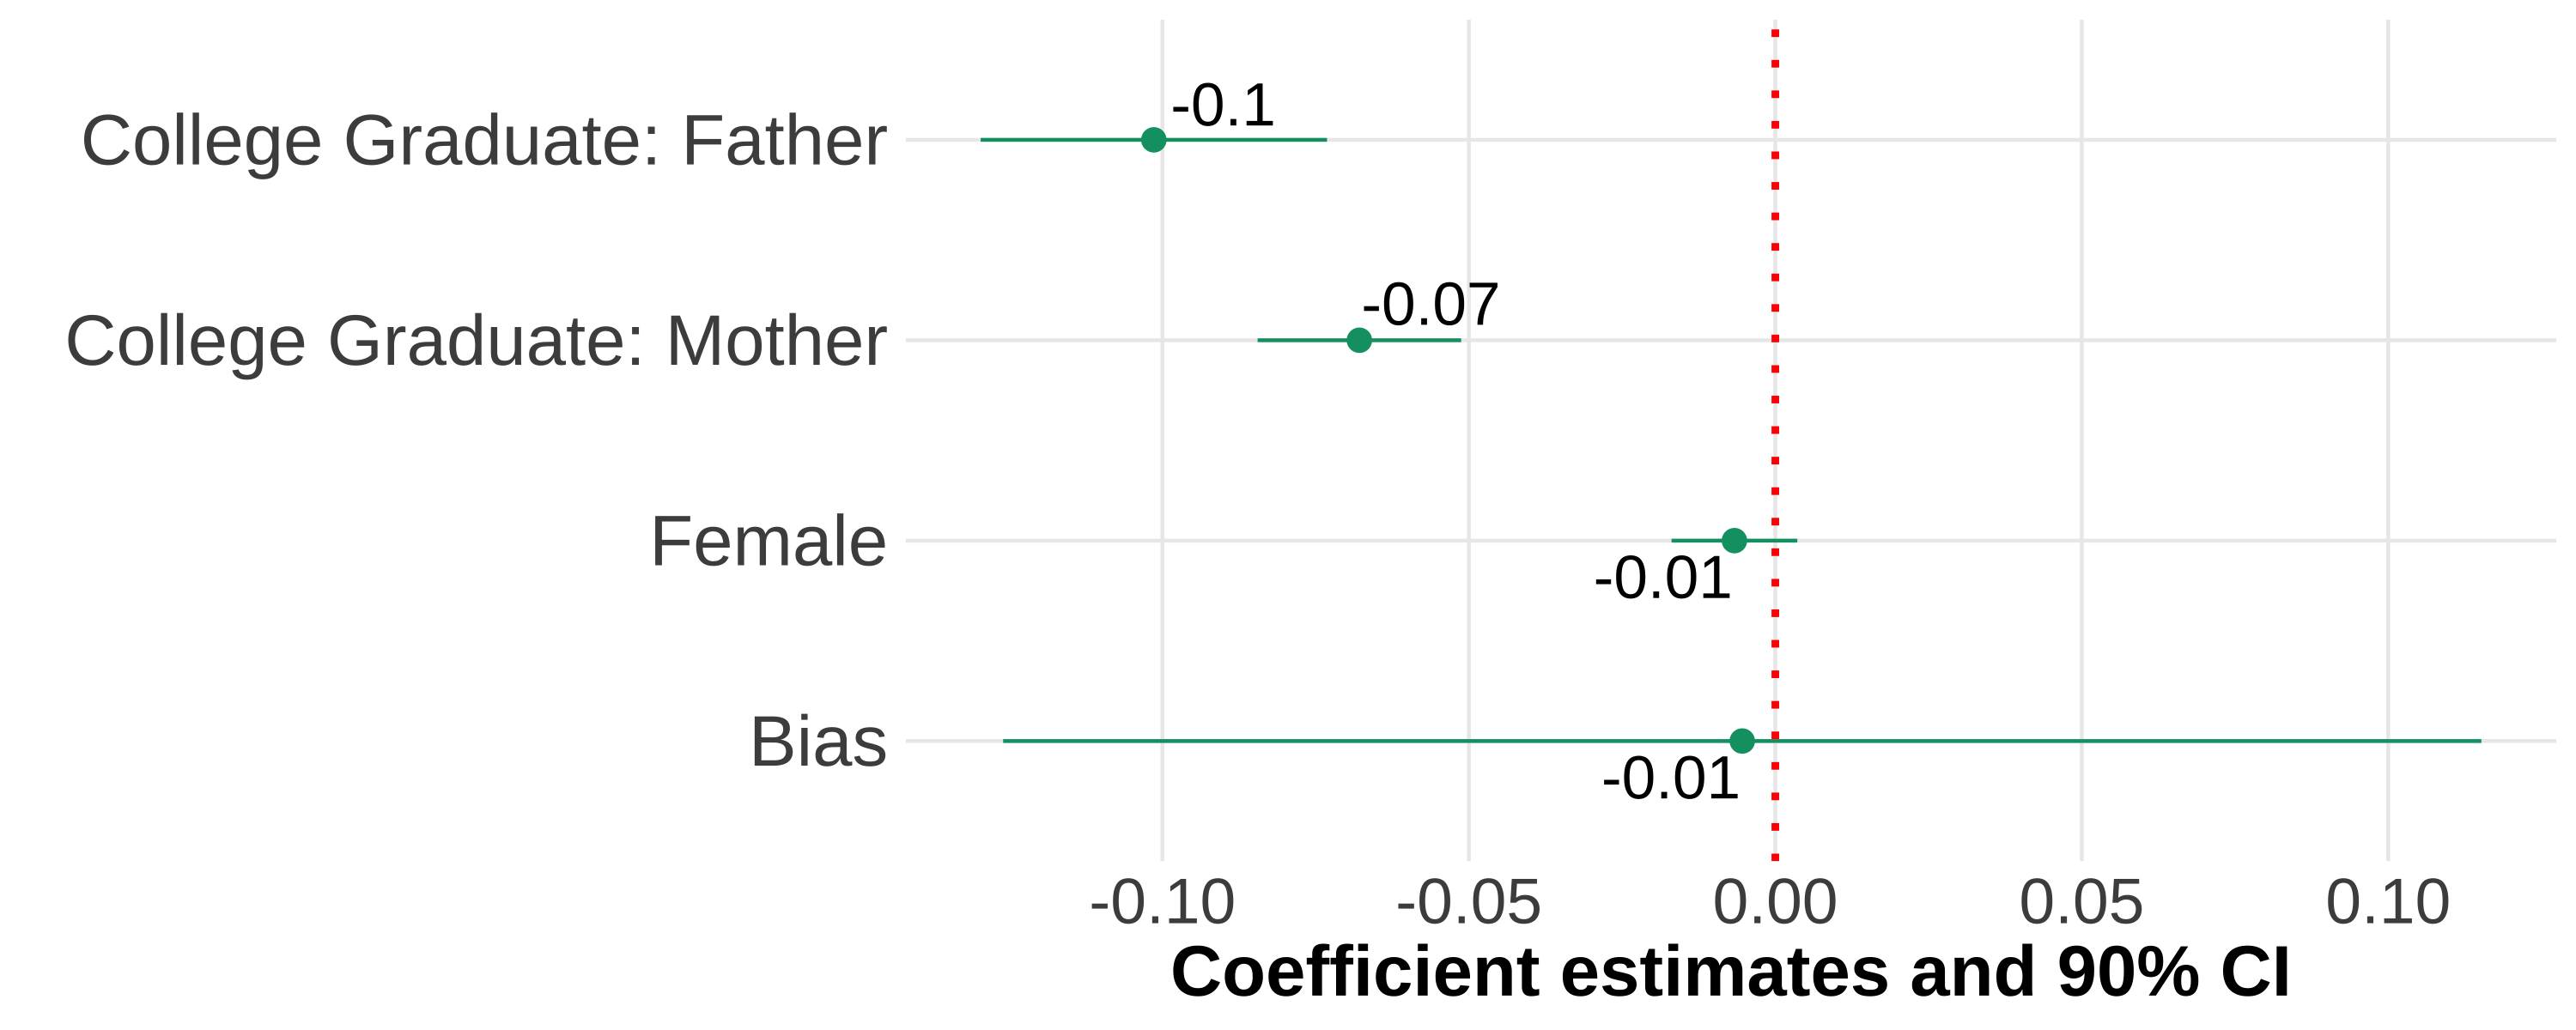
\includegraphics[width=.9\linewidth]{figure/by-parents-regs-hw.png}
\end{subfigure}
%Fourth Graph
\begin{subfigure}{.48\textwidth}
\caption{White Fathers-Hispanic Mothers}
\centering
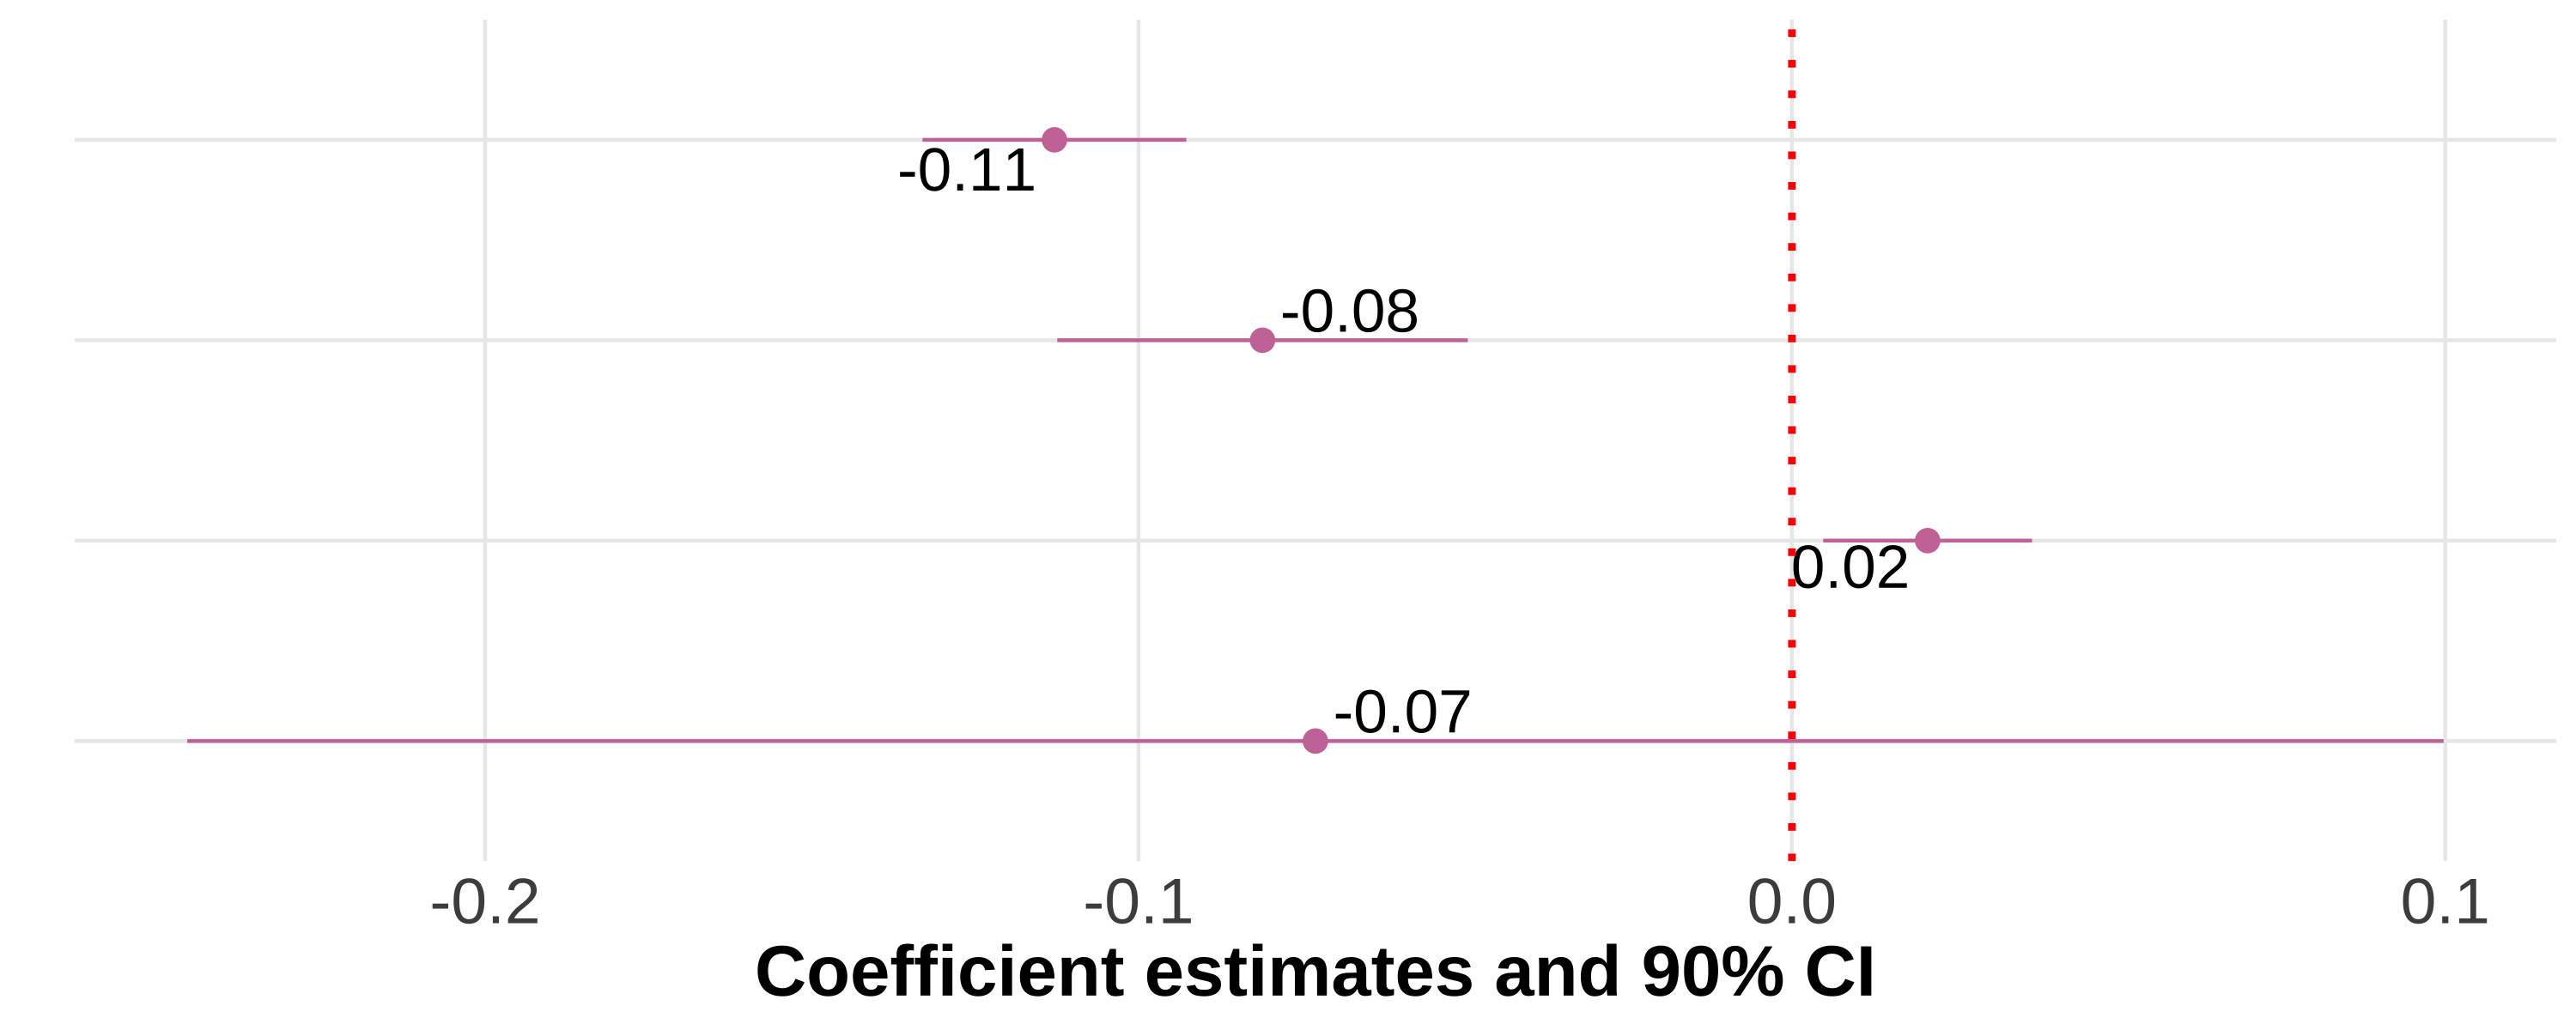
\includegraphics[width=.9\linewidth]{figure/by-parents-regs-wh.png}
\end{subfigure}
\flushleft\footnotesize{\note{I show four panels of estimating equation (\ref{eq:identity_reg_bias}). I include region $\times$ year fixed effects with controls for sex, quartic age, and parental education. The dependent variable is self-reported Hispanic identity and the independent variable is state-level bias. Each panel results from the same regression but on different samples divided by parents' types. Standard errors are clustered on the state level. The samples include second-generation Hispanic children ages 17 and below who live in intact families. Native-born second-generation Hispanic immigrant children with at least one parent born in a Spanish-speaking country.}}
\end{figure}
\end{center}

\subsubsection{Estimating the Relationship Between Bias, Interethnic Marriages, and Migration} % (fold)
\label{sub:the_determinants_of_hispanic_identity}

I will investigate the relationship between state-level bias and interethnic marriages. To this scope, the regressions for the estimation will be as follow:

\begin{align}
HH_{ist}^2 &= \beta_1^2 Bias_{st} + X_{ist}^2\pi + \gamma_{rt} 
            + \varepsilon_{ist} \nonumber \\
HW_{ist}^2 &= \beta_1^2 Bias_{st} + X_{ist}^2\pi + \gamma_{rt} 
            + \varepsilon_{ist}  \label{eq:inter-hw} \\
WH_{ist}^2 &= \beta_1^2 Bias_{st} + X_{ist}^2\pi + \gamma_{rt} 
            + \varepsilon_{ist}  \nonumber
\end{align}

Where $ HH_{ist}^2$, $ HW_{ist}^2$, and $ WH_{ist}^2$ are variables representing the type of parents of a second-generation Hispanic immigrant $i$ in state $s$ at time $t$. $HH_{ist}^2$ represents Hispanic-husband-Hispanic-wife couples, $HW_{ist}^2$ represents Hispanic-husband-White-wife couples, and $WH_{ist}^2$ represents White-husband-Hispanic-wife couples. $Bias_{st}$ is the average bias in state $s$ at time $t$, and $X_{ist}^2$ is a vector of partner-specific controls that would affect a marriage match that includes the wife's and husband's education, age, and year of immigration to the United States. 

There are two ways to estimate the effect of bias on the probability of an interethnic marriage forming. One way is by estimating equations (\ref{eq:inter-hw}) in three separate linear probability models. Another way is by estimating an ordered multinomial logistic regression. The dependent variable in the logistic regression will be an ordinal variable with a value of (1) zero corresponding to an endogenous marriage; (2) one corresponding to an interethnic Hispanic-husband-White-wife marriage; (3) two corresponding to an interethnic White-husband-Hispanic-wife marriage. The coefficient of interest from (\ref{eq:inter-hw}) is $\beta_1$, which estimates the effect of bias on the probability of forming an interethnic marriage. If $\beta_1 < 0$, higher bias is correlated with lower log odds of an interethnic marriage forming.

The relationship between bias and interehnic marriage could also be estimated using the following regression. 

\begin{align}
Interethnic_{ist}^2 &= \beta_1^2 Bias_{st} + X_{ist}^2\pi + \gamma_{rt} 
            + \varepsilon_{ist}  \label{eq:inter-interethnic} 
\end{align}

Where $Interethnic_{ist}^2$ is an indicator variable that is equal to one if a couple are interethnic, i.e. Hispanic husband-White wife or White husband-Hispanic wife. I could estimate equation (\ref{eq:inter-interethnic}) using a linear probability model. 

I am also interested in investigating the relationship between state-level bias and migration. For this purpose, I use the following specifications to estimate the relationship between state-level bias and migration:
\begin{align}
BirthPlaceMigration_{ist}^2 &= \beta_1^2 Bias_{st} 
                   + X_{ist}^2\pi + \gamma_{rt} 
                   + \varepsilon_{ist} \label{eq:migration-3} \\
BirthPlaceMigration_{ilb}^2 &= \beta_1^2 Bias_{lb} 
                   + X_{ilb}^2\pi + \gamma_{lb} 
                   + \varepsilon_{ilb} \label{eq:migration-4}
\end{align}

Where $BirthPlaceMigration_{ist}^2$ is an indicator variable equal to one if person $i$ in state $s$ at the interview $t$ lives in a state that is different from their state of birth and zero otherwise. $BirthPlaceMigration_{ilb}^2$ is an indicator variable that is equal to one if person $i$ in birth state $l$ does not currently live in the same state they lived in at the year of birth $b$ and zero otherwise. The analysis of equations (\ref{eq:migration-3}) and (\ref{eq:migration-4}) is restricted to second-generation Hispanic immigrants with both parents born in a Spanish speaking country. The coefficient of interest from the regressions is $\beta_1^2$, which captures the effect of bias on migration.

Furthermore, to study the relationship between bias and the migration variables introduced above, I use two different ways to define the bias variable. In the first definition from equation (\ref{eq:migration-3}), I estimate the relationship between the average bias in state $s$ at the time of the interview $t$ and $BirthPlaceMigration_{ist}^2$. In the Second specification from equation (\ref{eq:migration-4}), I estimate the relationship between the average bias in state of birth $l$ at the year of birth $b$ on $BirthPlaceMigration_{ilb}^2$. 

I will also estimate the selection into states based on bias levels. In other words, I want to estimate whether there's a relationship between the difference in state-level bias between the state $i$ is currently living in and their birth state and self-reported Hispanic identity. The estimation equation for the relationship is:

\begin{align}
Y_{ist} &= \beta_0 + \beta_1^2 Hispanic_{ist} +
                   X_{ist}^2\pi
                   + \varepsilon_{ist} \label{eq:migration-5}
\end{align}

Where $Y_{ist} \equiv Bias_{ist} -  Bias_{ilb}$, $Bias_{ist}$ is $i$'s state-level bias in state $s$ at the time of interview $t$, and  $Bias_{ilb}$ is $i$'s state-level bias in state of birth $l$ at the birth year $b$. The analysis is restricted to second-generation Hispanic immigrants with both parents born in a Spanish speaking country `that migrated from the state they were born in $b$ to another state $s$. The coefficient of interest is $\beta_1^2$, which captures whether a person that self-reports Hispanic identity self-selects and migrates into states that are more or less biased. For example, if $\beta_1^2>0$, then a person who self-reports Hispanic identity, compared to a person that does not, moves from states with less bias to a state with more bias.

\subsection{Results and Discussion} % (fold)
\label{sec:results}

In this section, I will present and discuss the results that I find to answer the following question. Is Hispanic self-identification associated with attitudes toward ethnic minorities in places individuals live in? Is the probability of an interethnic marriage associated with attitudes toward ethnic minorities? Are migration decisions associated with attitudes toward ethnic minorities in places they live in?

\subsection{Relationship between Attitudes and Identity}\label{sub:the_determinants_of_identity}

I find that state-level bias is negatively correlated with self-reported Hispanic identity. I find that a one standard deviation increase in state-level bias is correlated with 7 percentage points decrease in self-reported Hispanic identity among first-generation Hispanic immigrants and 13 percentage points decrease in self-reported Hispanic identity among second-generation Hispanic immigrants. I also find a negative correlation between bias and self-reported Hispanic identity in second-generation Hispanic immigrants children of parents born in a Spanish-speaking country and third-generation Hispanic immigrants children of four grandparents born in a Spanish-speaking country.

\begin{table}[H]

\caption{Relationship Between Bias and Self-Reported Hispanic Identity: By Generation \label{regtab-bygen-01}}
\centering
\resizebox{0.8\textwidth}{!}{
\begin{threeparttable}
\begin{tabular}[t]{lcccc}
\toprule
  & \specialcell{(1) \\ All Gens \\ $H_{ist}$} & \specialcell{(2) \\  First Gen \\ $H^1_{ist}$} & \specialcell{(3) \\  Second Gen \\ $H^2_{ist}$} & \specialcell{(4) \\  Third Gen \\ $H^3_{ist}$}\\
\midrule
Bias & \num{-0.10}** & \num{-0.07}* & \num{-0.13}** & \num{-0.02}\\
 & (\num{0.04}) & (\num{0.04}) & (\num{0.05}) & (\num{0.07})\\
Female & \num{0.00} & \num{0.00} & \num{0.00} & \num{0.00}\\
 & (\num{0.00}) & (\num{0.00}) & (\num{0.00}) & (\num{0.00})\\
College Graduate: Mother & \num{-0.05}*** & \num{-0.03}*** & \num{-0.06}*** & \num{-0.07}***\\
 & (\num{0.01}) & (\num{0.01}) & (\num{0.01}) & \vphantom{1} (\num{0.01})\\
College Graduate: Father & \num{-0.06}*** & \num{-0.06}*** & \num{-0.08}*** & \num{-0.08}***\\
 & (\num{0.01}) & (\num{0.01}) & (\num{0.01}) & (\num{0.01})\\
\midrule
N & \num{844481} & \num{85390} & \num{560100} & \num{198991}\\
Mean & \num{0.91} & \num{0.96} & \num{0.94} & \num{0.82}\\
Year $\times$ Region FE & X & X & X & X\\
\bottomrule
\multicolumn{5}{l}{\rule{0pt}{1em}* p $<$ 0.1, ** p $<$ 0.05, *** p $<$ 0.01}\\
\end{tabular}
\begin{tablenotes}
\small
\item[1] \footnotesize{Each column is an estimation of a heterogeneous effect of regression (\ref{eq:identity_reg_bias}) by 
                      generation with region × year fixed effects. 
                      I include controls for sex, quartic age, fraction of Hispanics in a state, and parental education.
                      I also added parents' (HH, HW, and WH) and grandparents' (HHHH, HHHW, HHWH, etc.) type dummy variables to the regression
                      on second and third generation immigrants, where H is objectively Hispanic (born in a Spanish Speaking Country) and W is objectively White (native born). 
                      Standard errors are clustered on the state level.}
\item[2] \footnotesize{The samples include children ages 17 and below who live in intact families. 
                      First-generation Hispanic immigrant children that were born in a 
                      Spanish speaking county. Native born second-generation Hispanic 
                      immigrant children with at least one parent born in a Spanish speaking 
                      country. Finally, native born third-generation Hispanic immigrant children 
                      with native born parents and at least one grandparent born in a Spanish 
                      speaking country.}
\item[3] \footnotesize{Data source is the 2004-2021 Current Population Survey.}
\end{tablenotes}
\end{threeparttable}}
\end{table}



I show the results of estimating equation (\ref{eq:identity_reg_bias}) using the different specifications by generation in figure (\ref{plot01-regression-gen}). Each panel evaluates a different specification with controls for parental education, sex, age, fraction of Hispanic people in a state, and region $\times$ year fixed effect. Panel (A) of the figure (\ref{plot01-regression-gen}) includes the results of estimating equation (\ref{eq:identity_reg_bias}) on the overall sample---i.e. pooling first-, second-, and third-generations together. I find that state-level bias is associated with a ten percentage points decrease in self-reported Hispanic identity. Panel (B) of figure (\ref{plot01-regression-gen}) includes the results of estimating equation (\ref{eq:identity_reg_bias}) on a sample of first-generation Hispanic immigrants. I find a negative relationship between state-level bias and self-reported Hispanic identity. A one standard deviation increase in bias is correlated with a six percentage points decrease in self-reported Hispanic identity. Panel (C) of figure (\ref{plot01-regression-gen}) includes the results of estimating equation (\ref{eq:identity_reg_bias}) on a sample of second-generation Hispanic immigrants. I find a negative relationship between state-level bias and self-reported Hispanic identity among second-generation immigrants. A one standard deviation increase in bias is correlated with a ten percentage points decrease in self-reported Hispanic identity. Panel (D) of figure (\ref{plot01-regression-gen}) includes the results of estimating equation (\ref{eq:identity_reg_bias}) on a sample of third-generation Hispanic immigrants. I find no statistically significant relationship between bias and self-reported Hispanic identity among third-generation immigrants. 

In table (\ref{regtab-byparent-01}), I provide the results of estimating equation (\ref{eq:identity_reg_bias}) on a sample of second-generation immigrants separately for each parent type---Spanish speaking country born father-Spanish speaking country born mother (HH), a native-born father-Spanish speaking country born mother (WH), and Spanish speaking country born father-native born mother (HW)---with region $\times$ year fixed effects. I find a significant negative correlation between bias and endogenous Hispanic identity among second-generation Hispanic immigrant children of endogamously Hispanic parents---both the father and mother were born in Spanish speaking country. A one standard deviation increase in bias is correlated with a 15 percentage points reduction in the self-reported Hispanic identity of second-generation Hispanic immigrant children of the Hispanic father-Hispanic mother (HH) (table \ref{regtab-byparent-01} column 2). The result is statistically significant. A one standard deviation increase in bias is correlated with a one percentage points decrease in the Hispanic identity of second-generation Hispanic immigrant children of the Hispanic father-White mother (HW) (table \ref{regtab-byparent-01} column 3). The result is statistically insignificant. A one standard deviation increase in bias is correlated with a seven percentage points decrease in the Hispanic identity of second-generation Hispanic immigrant children of the White father-Hispanic mother (WH) (table (\ref{regtab-byparent-01}) column 4). The results are statistically insignificant.

The results above indicate that attitudes are not correlated with the self-reported Hispanic identity of third-generation immigrants. One reason for this finding is that first and second-generation immigrants aim to integrate and assimilate into their new community, while third-generation immigrants are already assimilated. The results are consistent with the findings of \citet{abramitzkyImmigrantsAssimilateMore2020a} where they show that second-generation immigrants would change their foreign-sounding names to fit in and assimilate. 

Furthermore, I estimate another specification of equation (\ref{eq:identity_reg_bias}) by the number of grandparents that are objectively Hispanic---born in a Spanish-speaking country---and are third-generation Hispanic immigrants. For example, suppose a person has two grandparents born in a Spanish-speaking country. In that case, they have two `Hispanic' grandparents, and I will estimate a specification for all of those that belong to this group. The result of evaluating the effect of bias on people with one objectively Hispanic grandparent is in table (\ref{regtab-bygrandparents}) column (1), with two objectively Hispanic grandparents is in table (\ref{regtab-bygrandparents}) column (2), with three objectively Hispanic grandparents is in table (\ref{regtab-bygrandparents}) column (3), and with four objectively Hispanic grandparents is in table (\ref{regtab-bygrandparents}) column (4). I find a statistically significant relationship between and self-reported Hispanic identity among third-generation Hispanic immigrants with four objectively Hispanic grandparents. A one standard deviation increase in bias is associated with 14 percentage points decrease in the likelihood of a third-generation Hispanic immigrant with four objectively Hispanic grandparents to self-report Hispanic identity. Bias has no significant effect on children of interethnic grandparents.  

\begin{table}[H]

\caption{Relationship Between Bias and Self-Reported Hispanic identity Among Second-Generation Hispanic Immigrants: By Parental Type \label{regtab-byparent-01}}
\centering
\resizebox{0.9\textwidth}{!}{
\begin{threeparttable}
\begin{tabular}[t]{lcccc}
\toprule
\multicolumn{1}{c}{Parents Type} & \multicolumn{1}{c}{All} & \multicolumn{1}{c}{\makecell[c]{Both Parents \\ from Spanish \\ Speaking Country \\ (HH)}} & \multicolumn{1}{c}{\makecell[c]{Father \\ from Spanish \\ Speaking Country \\ (HW)}} & \multicolumn{1}{c}{\makecell[c]{Mother  \\ from Spanish \\ Speaking Country \\ (WH)}} \\
\cmidrule(l{3pt}r{3pt}){1-1} \cmidrule(l{3pt}r{3pt}){2-2} \cmidrule(l{3pt}r{3pt}){3-3} \cmidrule(l{3pt}r{3pt}){4-4} \cmidrule(l{3pt}r{3pt}){5-5}
  & \specialcell{(1) \\ $H^2_{ist}$} & \specialcell{(2) \\ $H^2_{ist}$} & \specialcell{(3) \\ $H^2_{ist}$} & \specialcell{(4) \\ $H^2_{ist}$}\\
\midrule
Bias & \num{-0.13}** & \num{-0.15}** & \num{-0.01} & \num{-0.07}\\
 & (\num{0.05}) & (\num{0.06}) & (\num{0.07}) & (\num{0.10})\\
Female & \num{0.00} & \num{0.00} & \num{-0.01} & \num{0.02}**\\
 & (\num{0.00}) & (\num{0.00}) & (\num{0.01}) & (\num{0.01})\\
College Graduate: Mother & \num{-0.06}*** & \num{-0.04}*** & \num{-0.07}*** & \num{-0.08}***\\
 & (\num{0.01}) & (\num{0.01}) & (\num{0.01}) & (\num{0.02})\\
College Graduate: Father & \num{-0.08}*** & \num{-0.04}*** & \num{-0.10}*** & \num{-0.11}***\\
 & (\num{0.01}) & (\num{0.01}) & (\num{0.02}) & (\num{0.01})\\
\midrule
N & \num{560100} & \num{405116} & \num{88421} & \num{66563}\\
Year $\times$ Region FE & X & X & X & X\\
Mean & \num{0.94} & \num{0.96} & \num{0.9} & \num{0.83}\\
\bottomrule
\multicolumn{5}{l}{\rule{0pt}{1em}* p $<$ 0.1, ** p $<$ 0.05, *** p $<$ 0.01}\\
\end{tabular}
\begin{tablenotes}
\small
\item[1] \footnotesize{Each column is an estimation of a heterogeneous effect of regression (\ref{eq:identity_reg_bias}) by 
                      type of parents with region × year fixed effects. 
                      I include controls for sex, quartic age, fraction of Hispanics in a state, and parental education.
                      Standard errors are clustered on the state level.}
\item[2] \footnotesize{The samples include second-generation Hispanic children ages 17 and below who live in intact families. 
                      Native born second-generation Hispanic 
                      immigrant children with at least one parent born in a Spanish speaking 
                      country.}
\item[3] \footnotesize{Column (1) includes the results to regression (\ref{eq:identity_reg_bias}) on all second-generation immigrants, 
                                        column (2) includes the results to regression (\ref{eq:identity_reg_bias}) on second-generation immigrants that who has a father and mother that were born in a Spanish speaking country (HH),
                                        column (3) includes the results to regression (\ref{eq:identity_reg_bias}) on second-generation immigrants that who has a father that was born in a Spanish speaking country and a native born mother (HW), and
                                        column (4) includes the results to regression (\ref{eq:identity_reg_bias}) on second-generation immigrants that who has a native born father and a mother that was born in a Spanish speaking country (WH).}
\item[4] \footnotesize{Data source is the 2004-2021 Current Population Survey.}
\end{tablenotes}
\end{threeparttable}}
\end{table}


\begin{center}
\begin{figure}[H]
\caption{Relationship Between Bias and Self-reported Identity on Second-Generation Hispanics: Interaction}
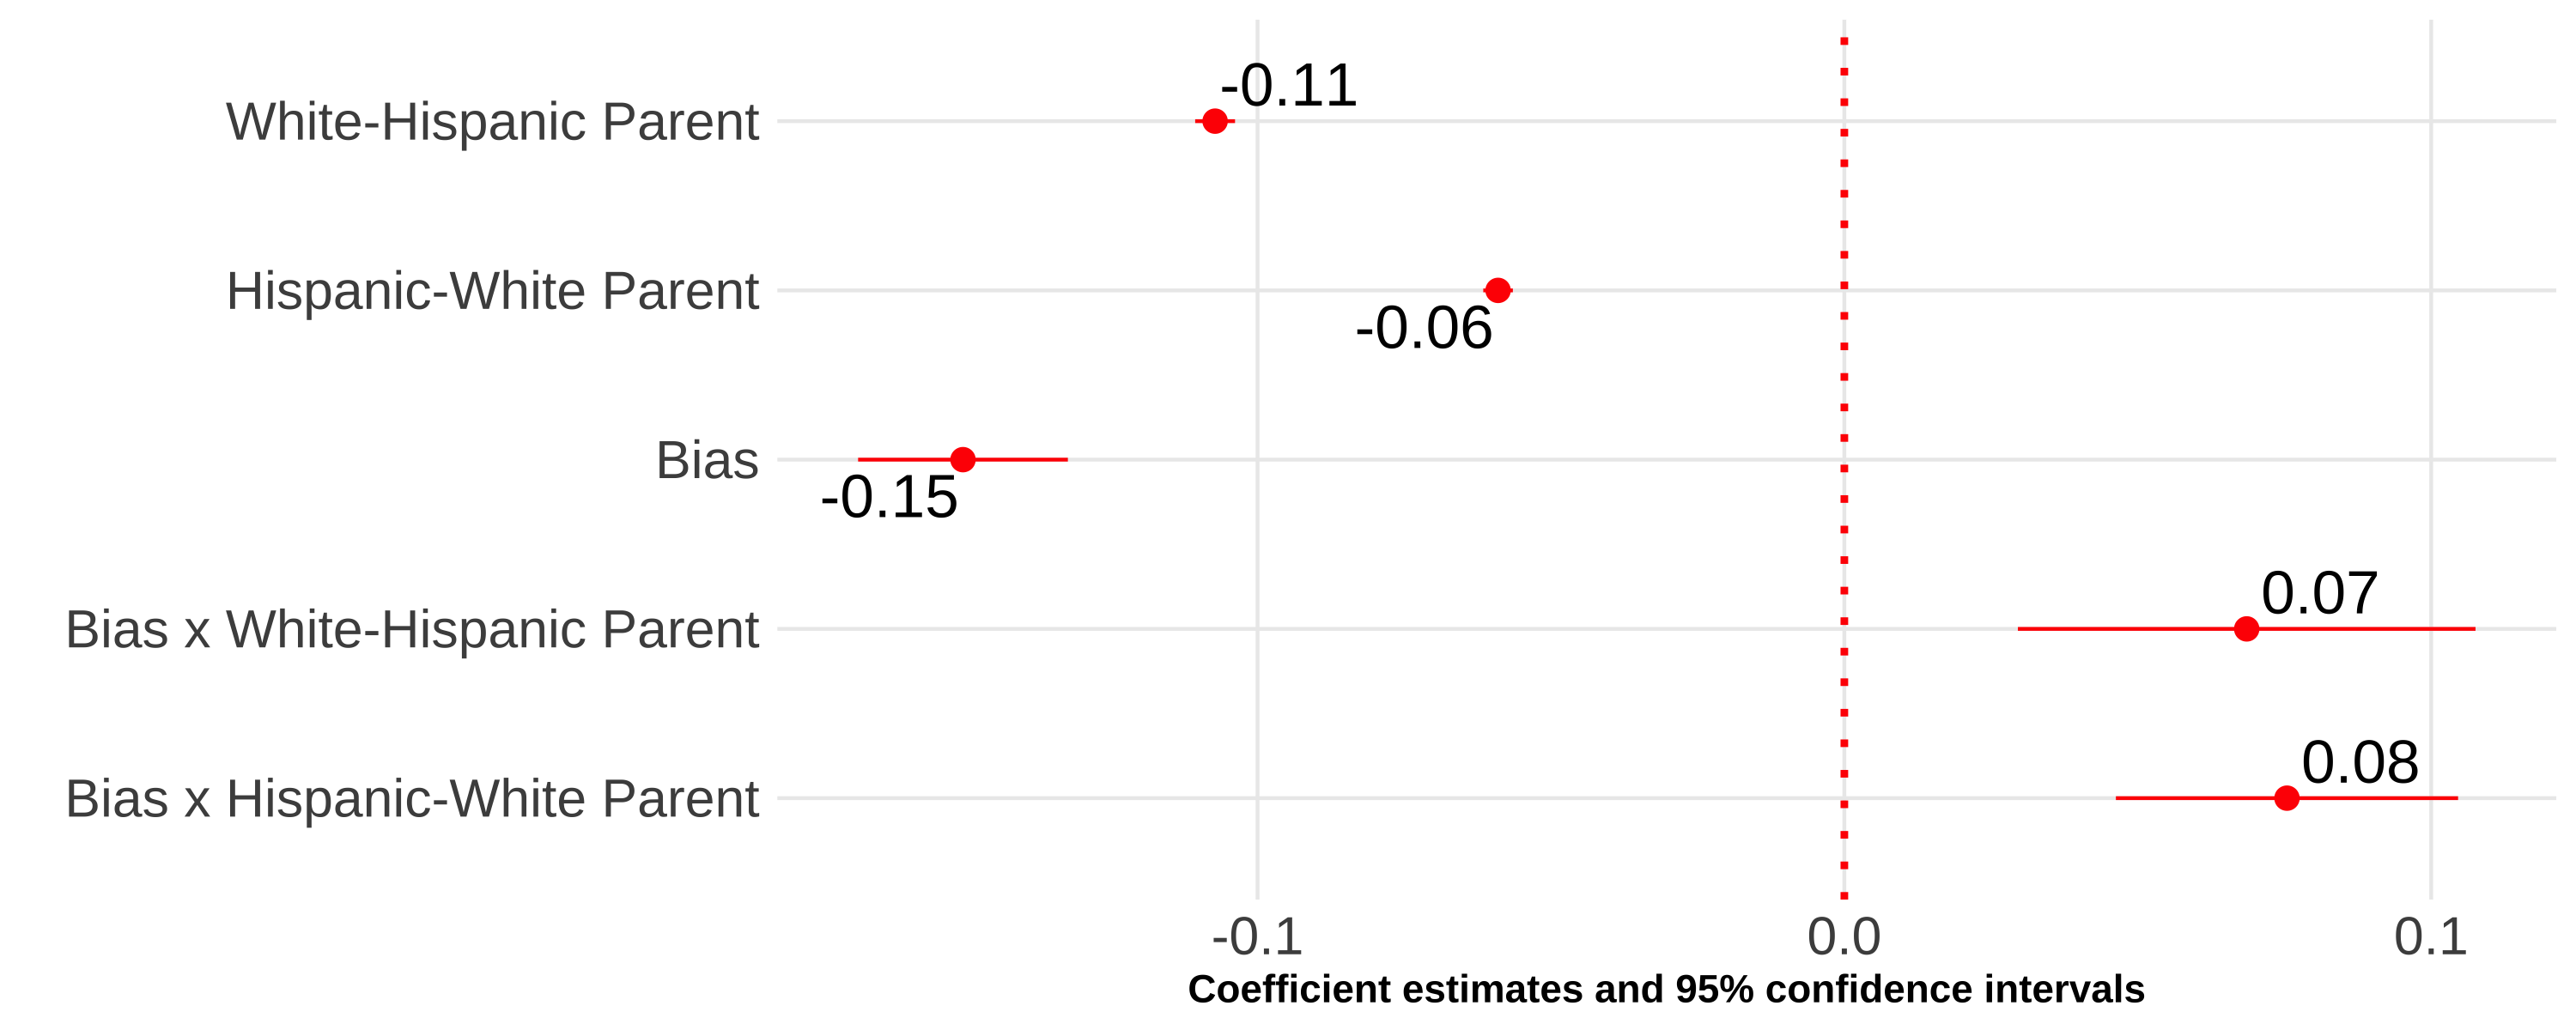
\includegraphics[width=\textwidth]{figure/skin-iat-regression-interaction-bygen-plot-second.png} 
\label{fig:reg-interaction-second}
\flushleft\footnotesize{\note{I show four panels of estimating equation (\ref{eq:identity_reg_bias_interaction_2}). I include region $\times$ year fixed effects with controls for sex, quartic age, faction of Hispanics in a state, and parental education. Each panel is the results from the same regression but is presented with different combinations of grandparents' types. Robust standard errors are reported. The samples include second-generation Hispanic children ages 17 and below who live in intact families. Native-born second-generation Hispanic immigrant children with at least one parent born in a Spanish-speaking country.}}
\end{figure}
\end{center}

\begin{table}[H]

\caption{Relationship Between Bias and Self-Reported Hispanic identity Among Third-Generation Hispanic Immigrants: By Grandparental Type \label{regtab-bygrandparents}}
\centering
\resizebox{0.8\textwidth}{!}{
\begin{threeparttable}
\begin{tabular}[t]{lcccc}
\toprule
\multicolumn{1}{c}{ } & \multicolumn{4}{c}{Number of Hispanic Grandparents} \\
\cmidrule(l{3pt}r{3pt}){2-5}
  & \specialcell{(1) \\ One} & \specialcell{(2) \\ Two} & \specialcell{(3) \\ Three} & \specialcell{(4) \\ Four}\\
\midrule
Bias & \num{-0.04} & \num{0.03} & \num{0.19} & \num{-0.14}*\\
 & (\num{0.11}) & (\num{0.09}) & (\num{0.26}) & (\num{0.07})\\
Female & \num{-0.01} & \num{0.00} & \num{-0.01} & \num{0.00}\\
 & (\num{0.01}) & (\num{0.01}) & (\num{0.01}) & (\num{0.01})\\
College Graduate: Mother & \num{-0.11}*** & \num{-0.07}*** & \num{0.02} & \num{-0.02}\\
 & (\num{0.03}) & (\num{0.02}) & (\num{0.02}) & (\num{0.01})\\
College Graduate: Father & \num{-0.11}*** & \num{-0.08}*** & \num{0.02} & \num{-0.03}*\\
 & (\num{0.03}) & (\num{0.01}) & (\num{0.01}) & (\num{0.01})\\
\midrule
N & \num{55051} & \num{74100} & \num{12194} & \num{57646}\\
Year $\times$ Region FE & X & X & X & X\\
\bottomrule
\multicolumn{5}{l}{\rule{0pt}{1em}* p $<$ 0.1, ** p $<$ 0.05, *** p $<$ 0.01}\\
\end{tabular}
\begin{tablenotes}
\small
\item[1] \footnotesize{Each column is an estimation of equation (\ref{eq:identity_reg_bias}) restricted to third-generation Hispanic immigrants by 
                      number of Hispanic grandparents with region × year fixed effects. 
                      I include controls for sex, quartic age, fraction of Hispanics in a state, and parental education.
                      Standard errors are clustered on the state level.}
\item[2] \footnotesize{The samples include third-generation Hispanic children ages 17 and below who live in intact families. 
                      Native born third-generation Hispanic 
                      immigrant children with at least one grandparent born in a Spanish speaking 
                      country.}
\item[3] \footnotesize{Data source is the 2004-2021 Current Population Survey.}
\end{tablenotes}
\end{threeparttable}}
\end{table}



\begin{figure}[H]
\centering
\caption{Relationship Between Bias and Self-reported Identity on third-generation Hispanics: Interaction}
\label{fig:reg-interaction-third}
\begin{subfigure}{.48\textwidth}
\centering
\caption{White Paternal Grandfather and White Paternal Grandmother Combinations}
\label{fig:reg-interaction-third-a}
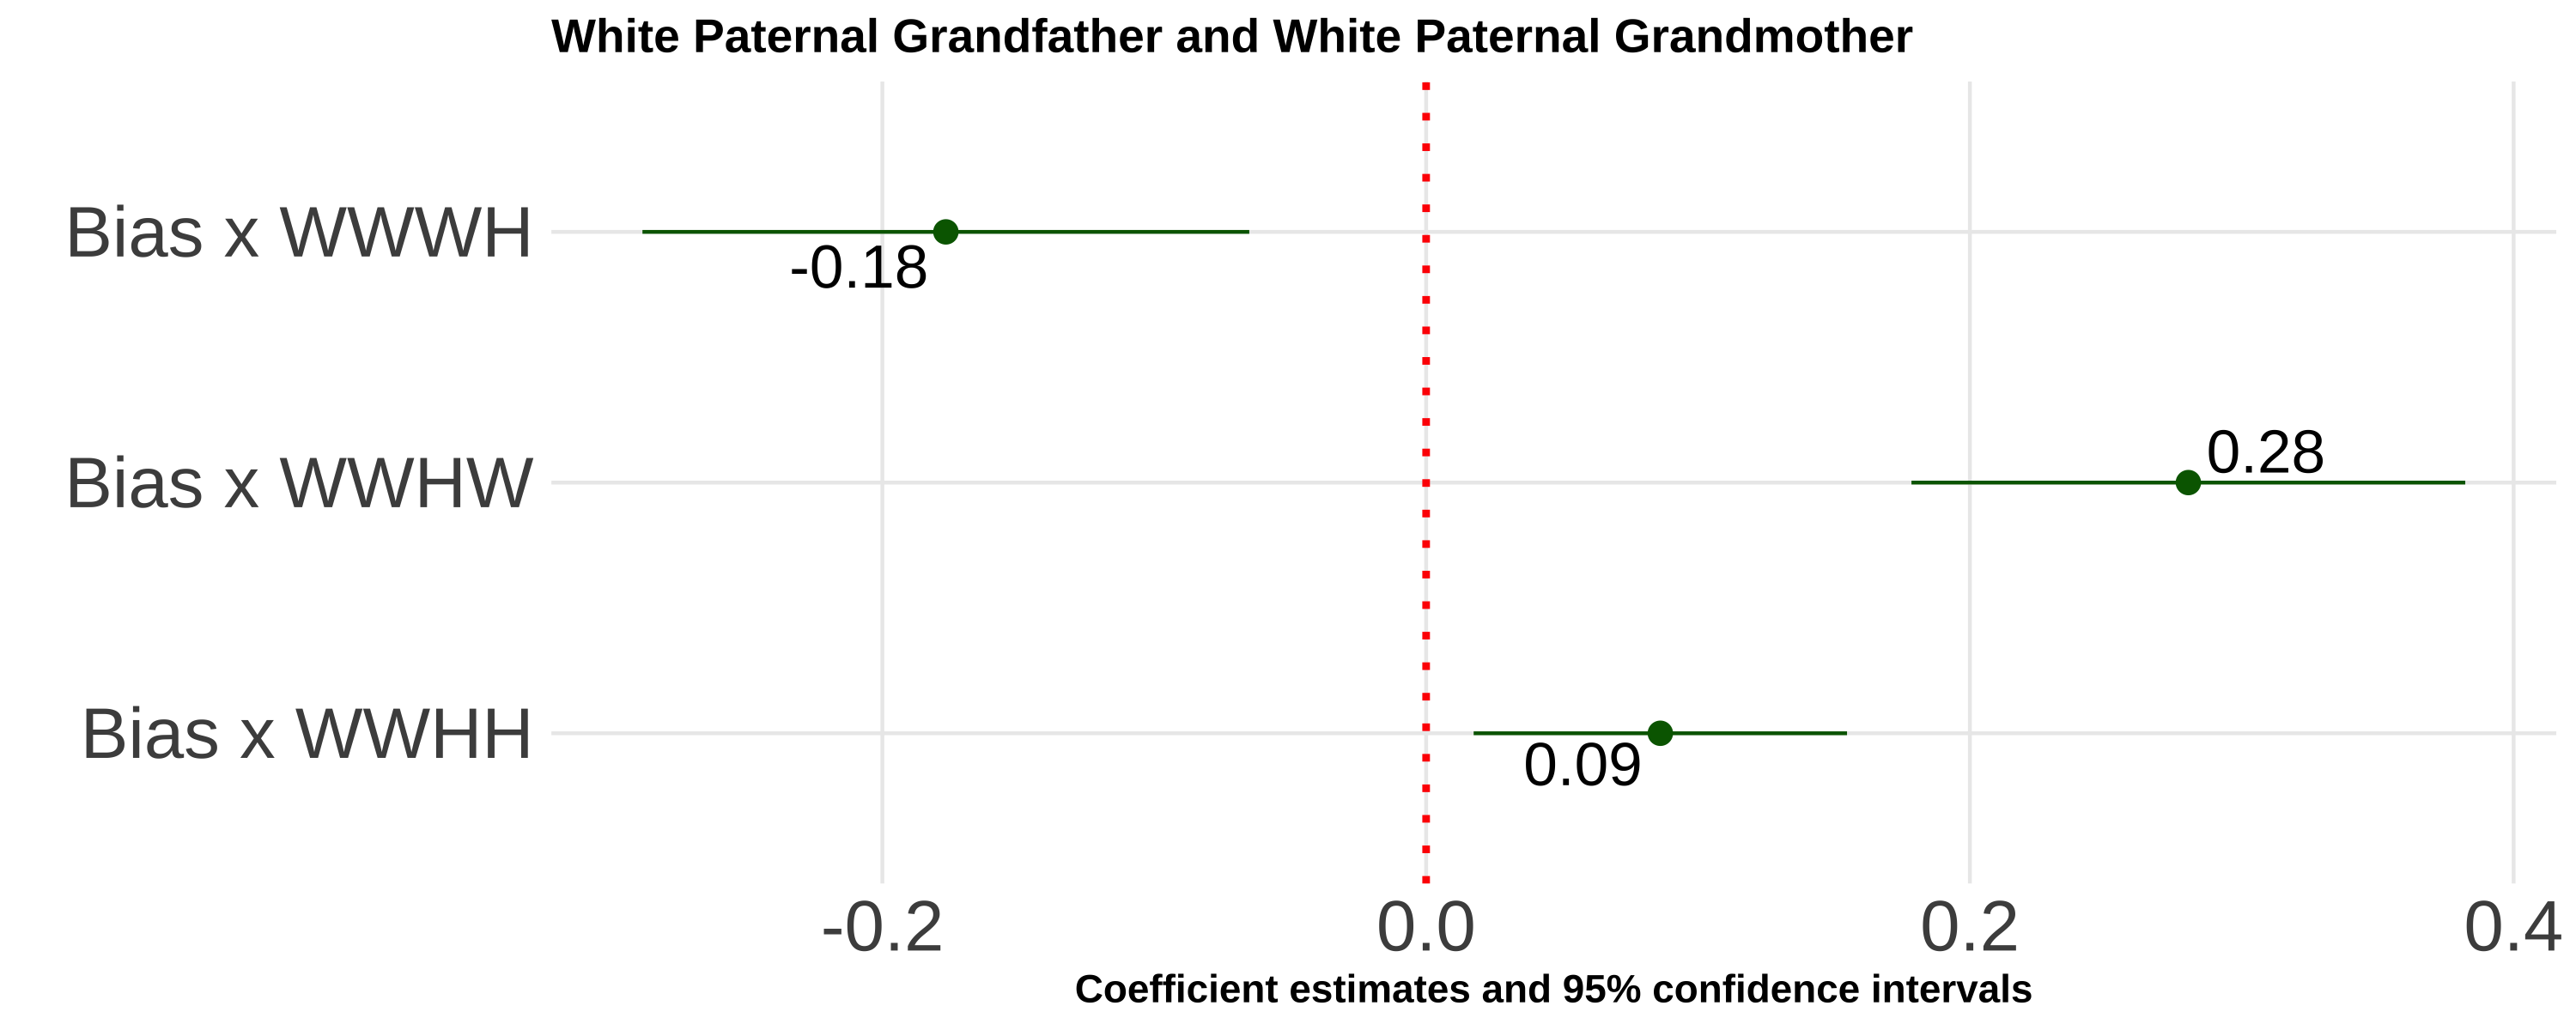
\includegraphics[width=.9\linewidth]{figure/skin-iat-regression-interaction-bygen-plot-WW.png}
\end{subfigure}
\centering
%Second graph
\begin{subfigure}{.48\textwidth}
\centering
\caption{Hispanic Paternal Grandfather and Hispanic Paternal Grandmother Combinations}
\label{fig:reg-interaction-third-b}
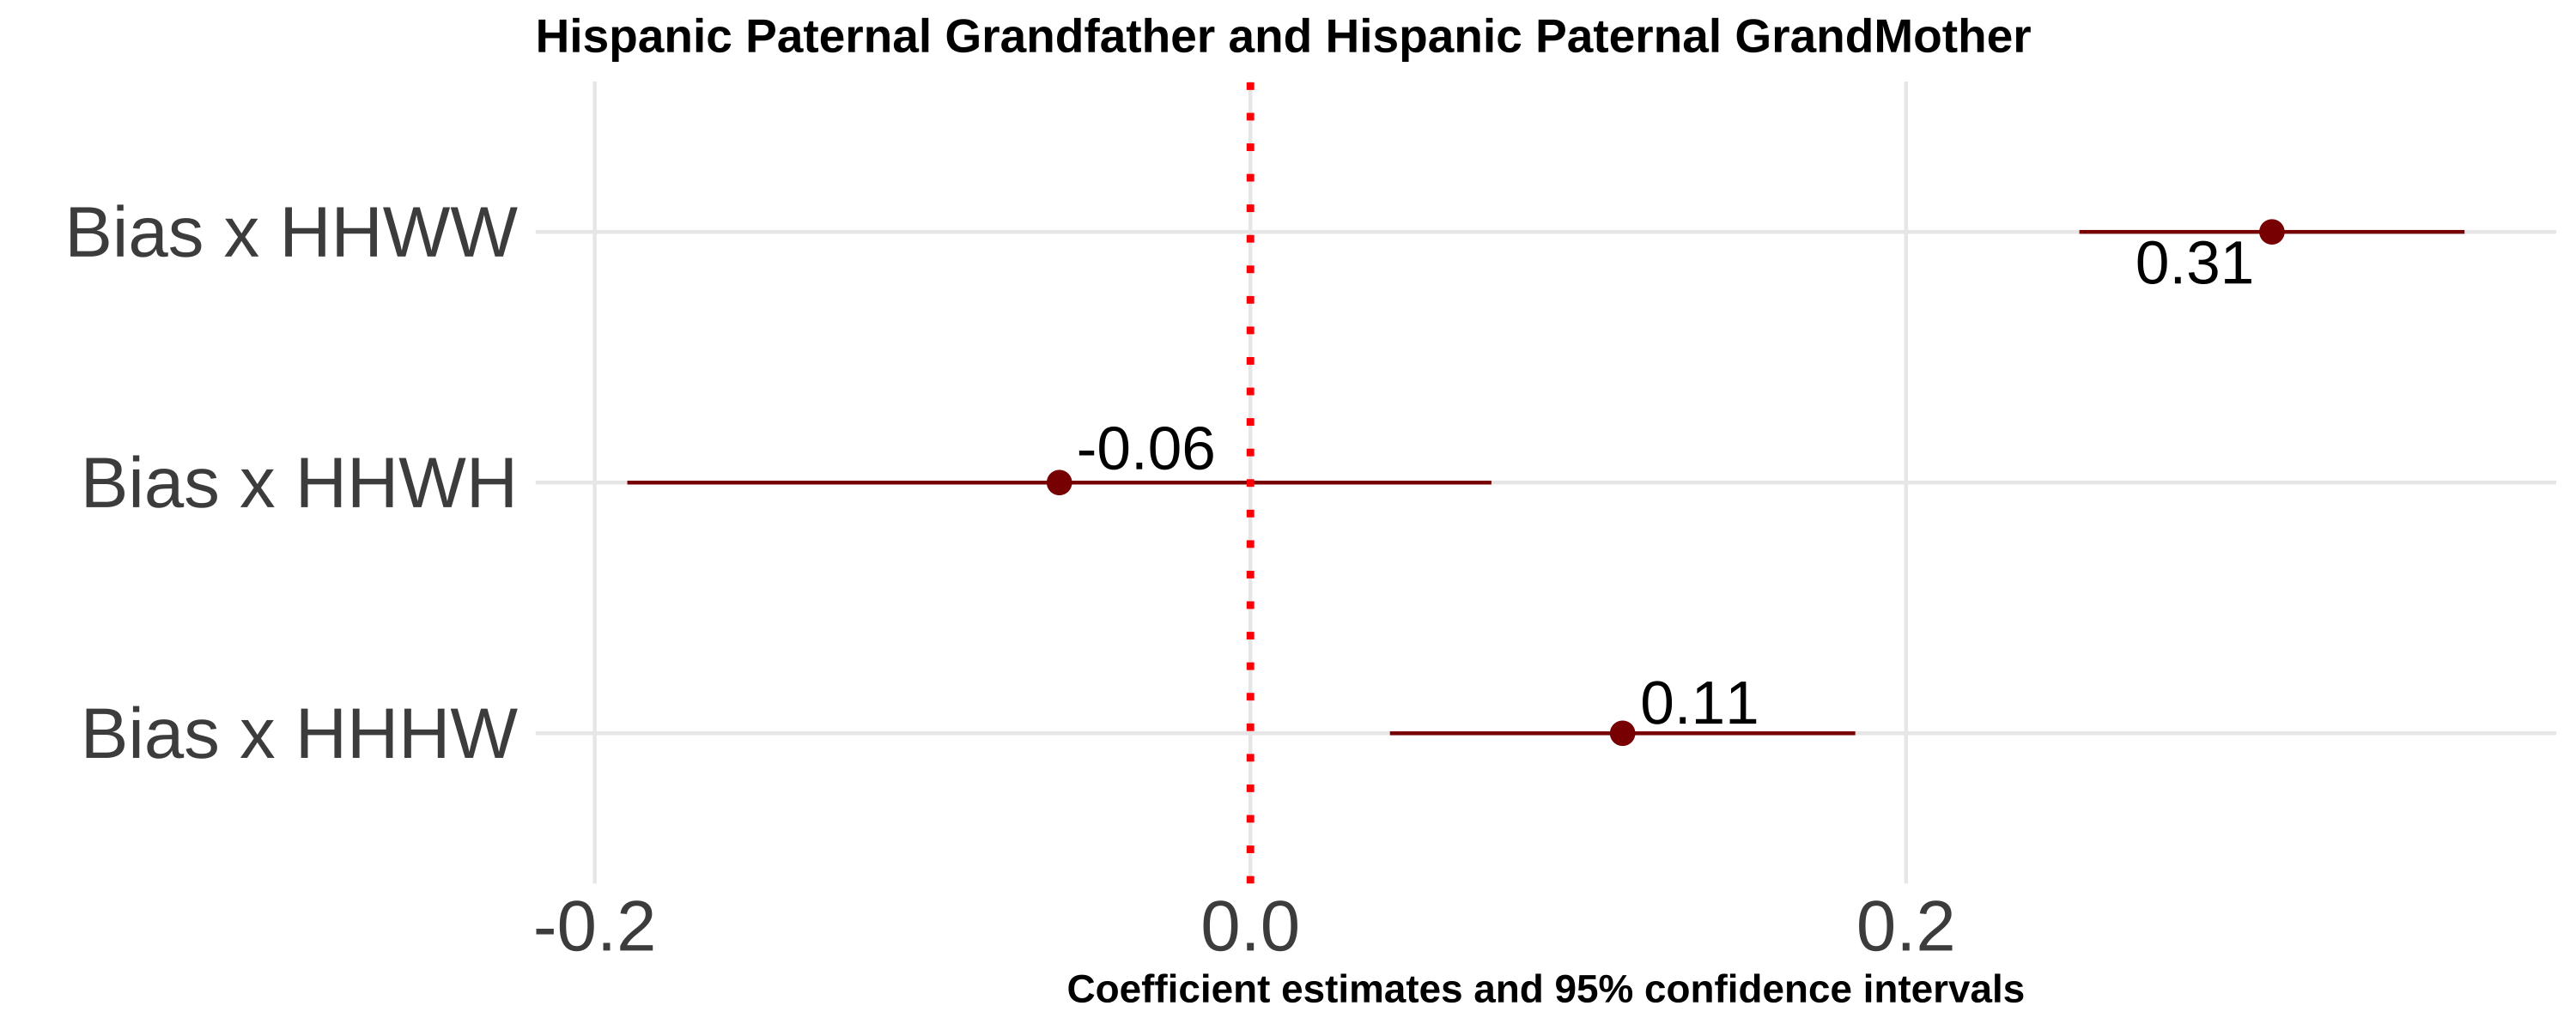
\includegraphics[width=.9\linewidth]{figure/skin-iat-regression-interaction-bygen-plot-HH.png}
\end{subfigure}
%Third
\begin{subfigure}{.48\textwidth}
\centering
\caption{Hispanic Paternal Grandfather and White Paternal Grandmother Combinations}
\label{fig:reg-interaction-third-c}
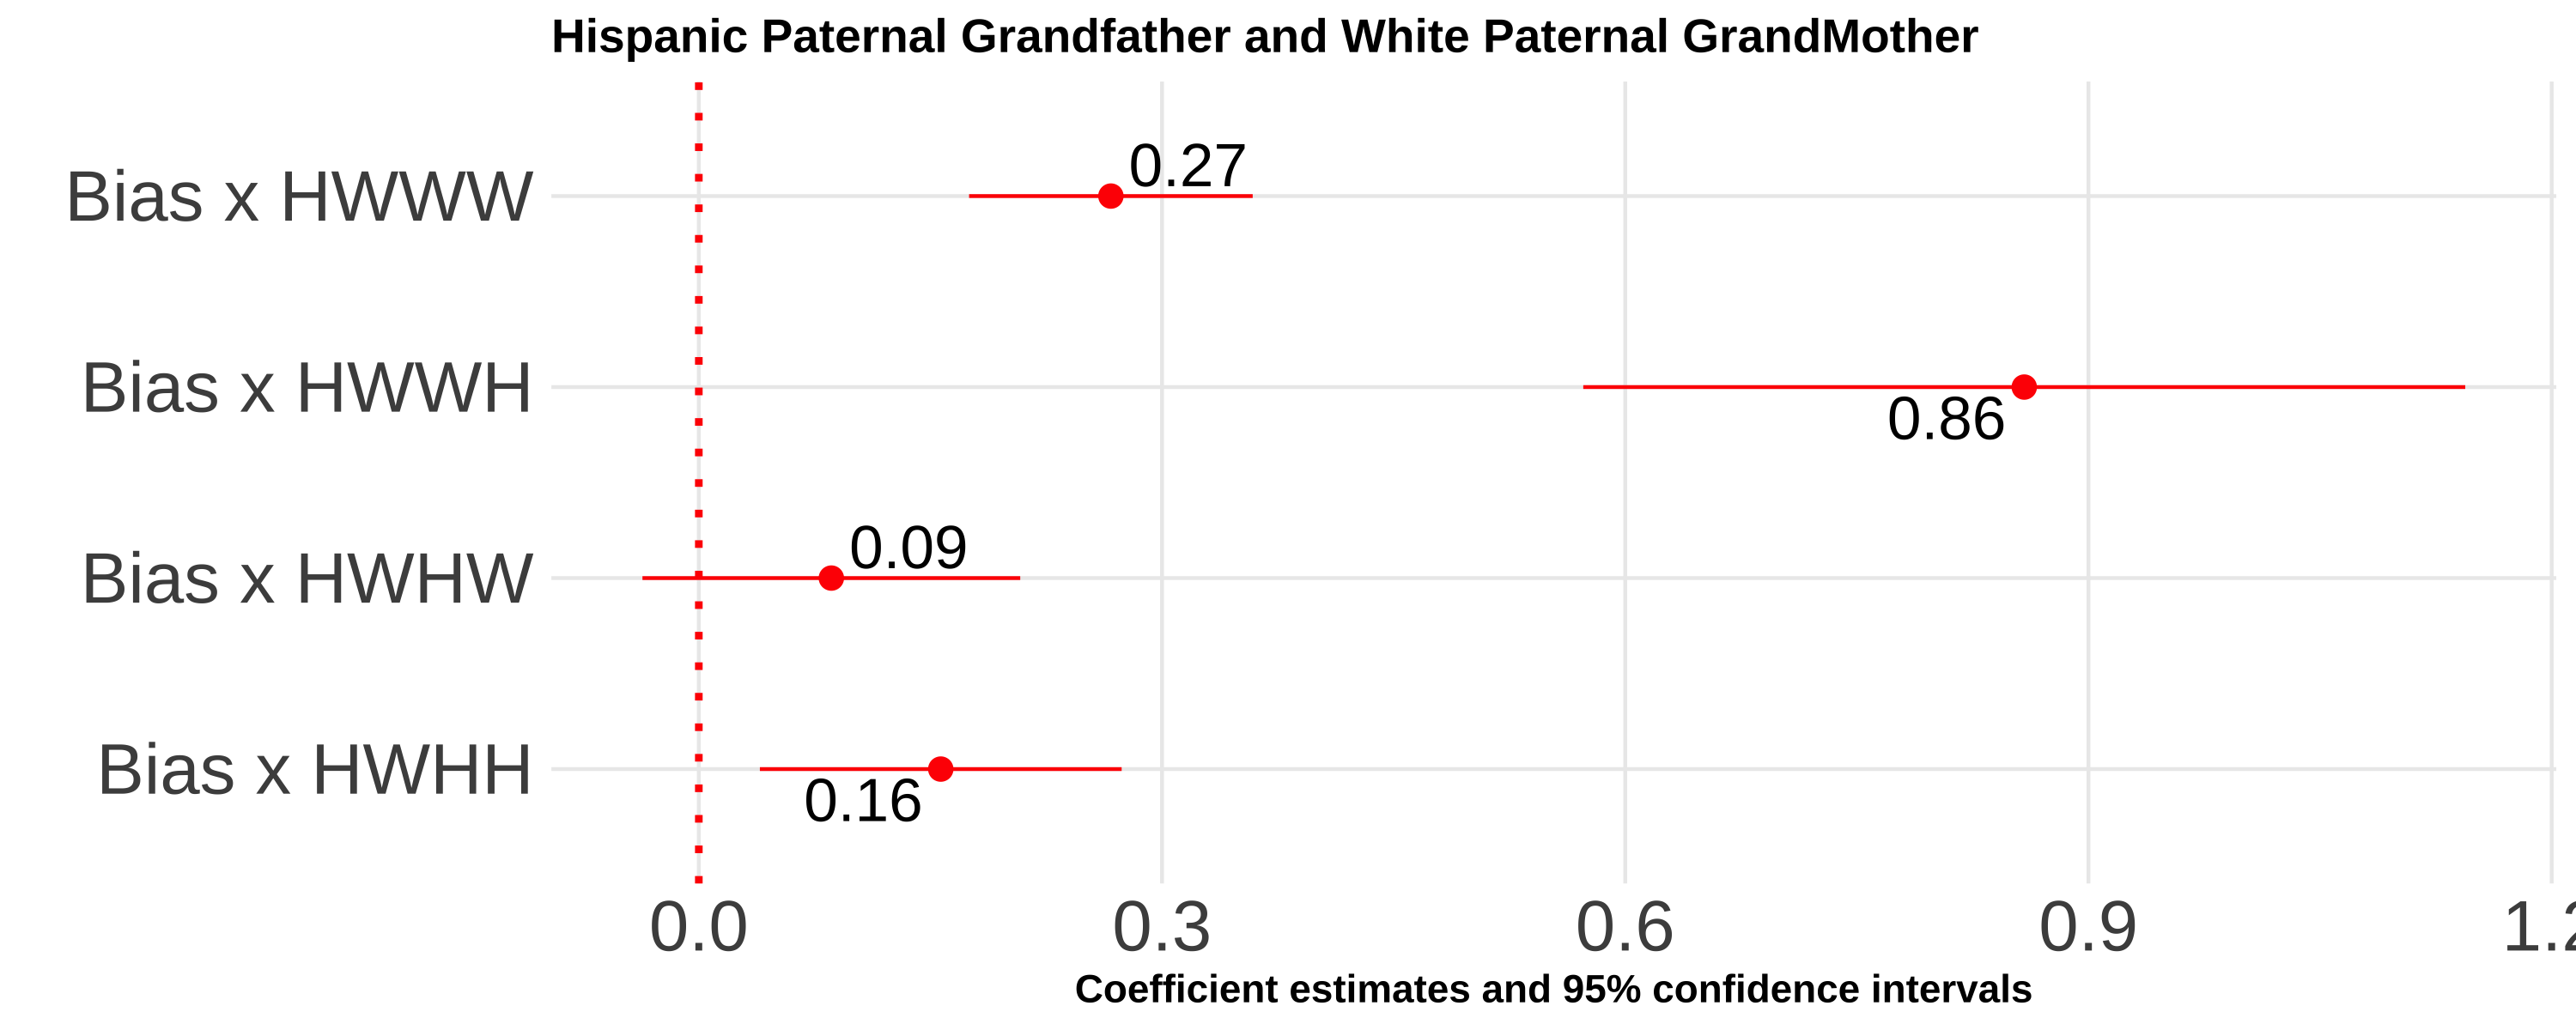
\includegraphics[width=.9\linewidth]{figure/skin-iat-regression-interaction-bygen-plot-HW.png}
\end{subfigure}
% Fourth
\begin{subfigure}{.48\textwidth}
\centering
\caption{White Paternal Grandfather and Hispanic Paternal Grandmother Combinations}
\label{fig:reg-interaction-third-d}
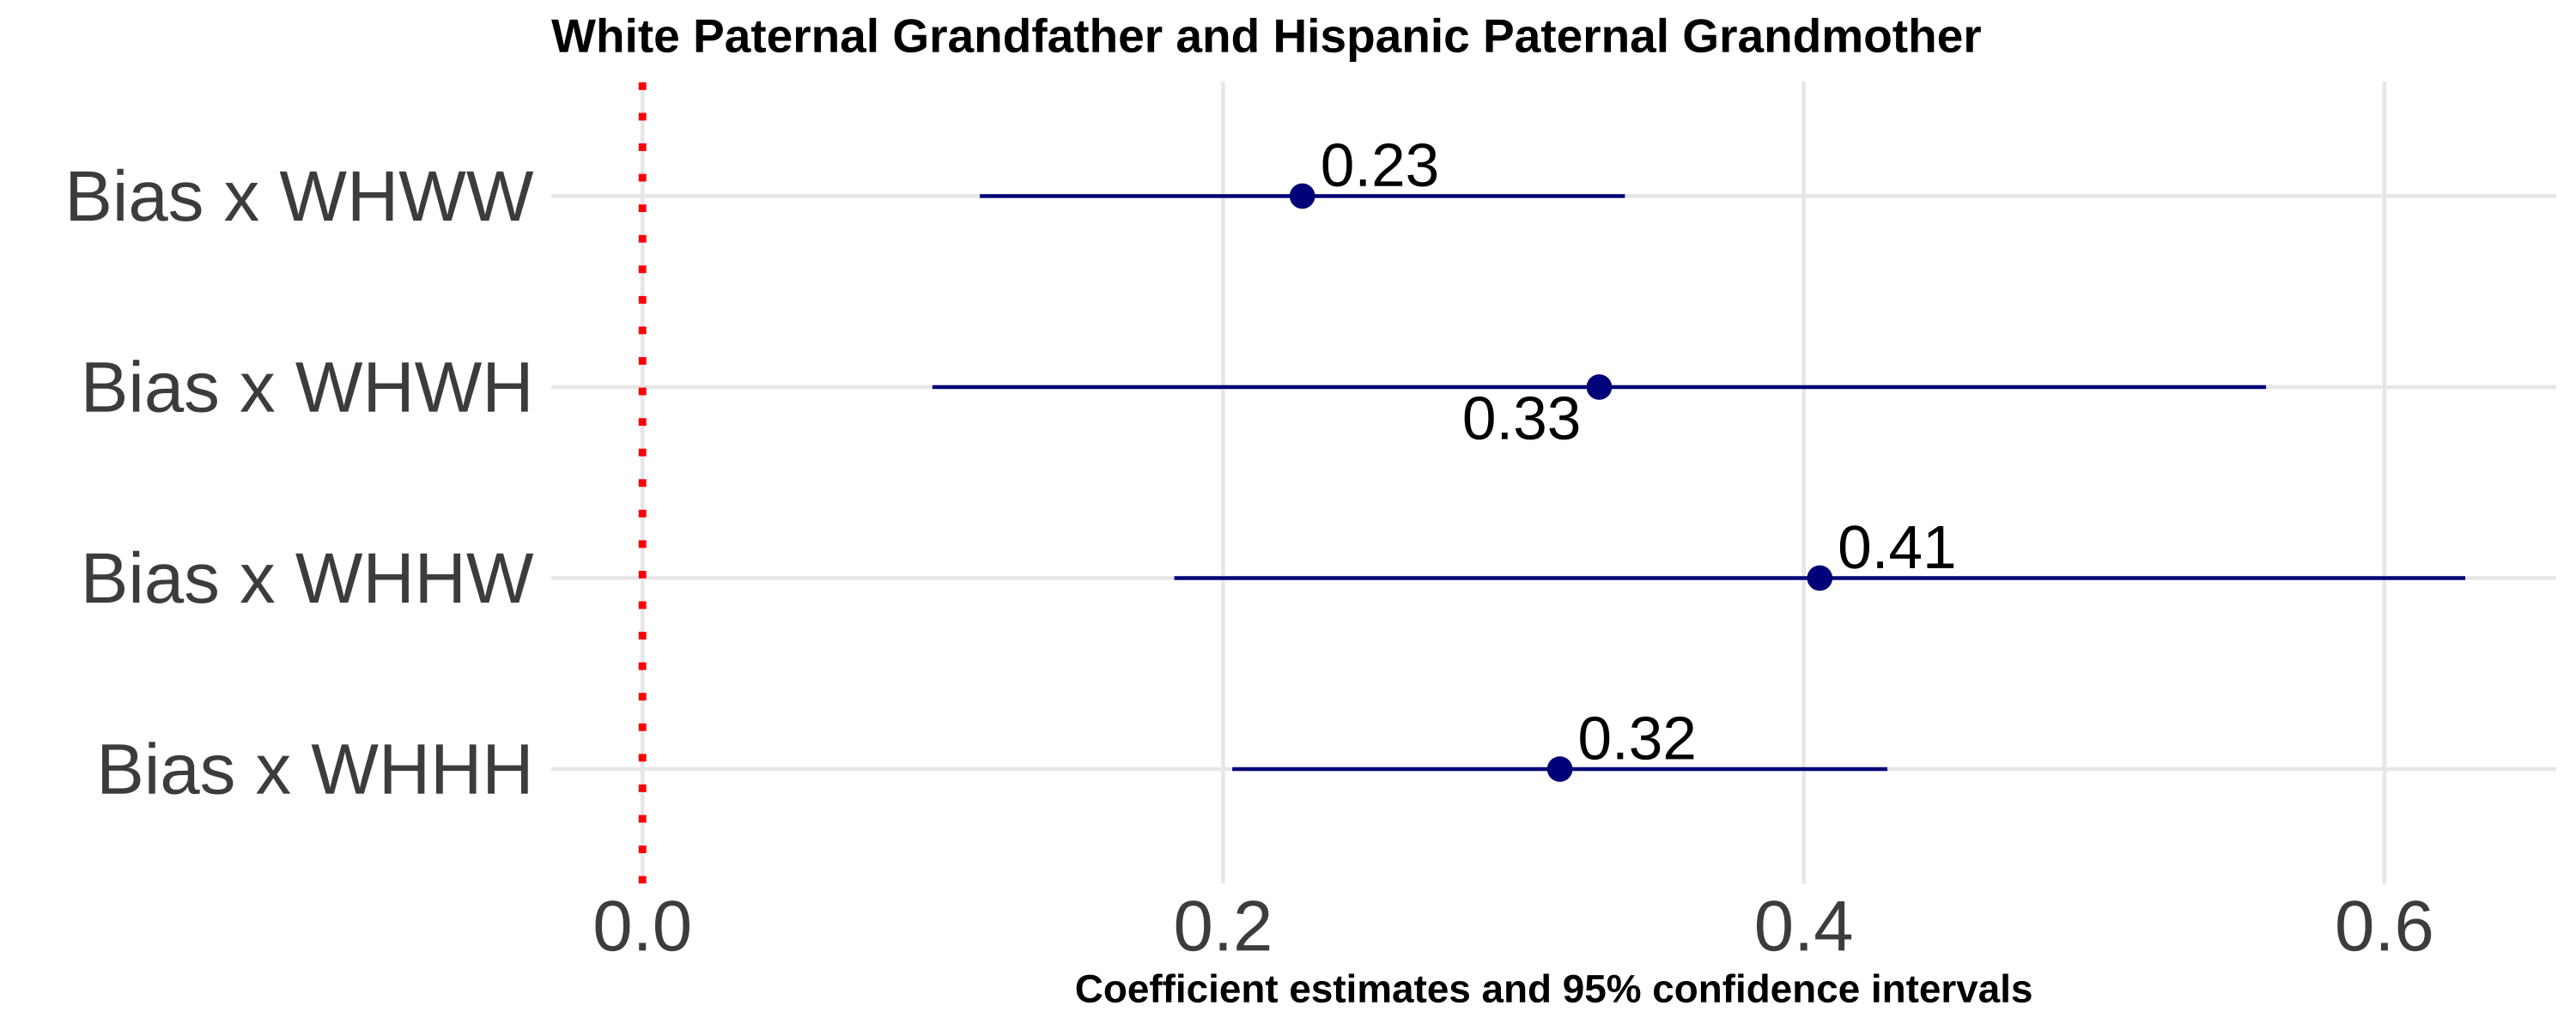
\includegraphics[width=.9\linewidth]{figure/skin-iat-regression-interaction-bygen-plot-WH.png}
\end{subfigure}
\flushleft\footnotesize{\note{I show four panels of estimating equation (\ref{eq:identity_reg_bias_interaction_3}). I include region $\times$ year fixed effects with controls for sex, quartic age, and parental education. Each panel results from the same regression but is presented by different combinations of grandparents' types. The syntax of the grandparents' type consists of four letters. The first letter represents the paternal grandfather, the second letter represents the paternal grandmother, the third letter represents the maternal grandfather, and the fourth letter represents the maternal grandmother. A grandparent would be of type \textit{H} if they were born in a Spanish-speaking country and of type \textit{W} if they were native-born. Robust standard errors are reported. The samples include third-generation Hispanic children ages 17 and below who live in intact families. Third-generation Hispanic immigrant children with native-born parents and at least one grandparent born in a Spanish-speaking country.}}
\end{figure}

I estimate the heterogeneous relationship between bias and self-reported Hispanic identity by parents' types of equation (\ref{eq:identity_reg_bias_interaction_2}) and show the results in figure (\ref{fig:reg-interaction-second}). This specification estimates the heterogeneous effect of bias on a sample of second-generation immigrants by parental type. Moreover, I find a statistically significant positive heterogeneous relationship between bias and parents on self-reported Hispanic identity. I find that a one standard deviation increase in state-level bias correlates with a seven percentage points increase in Hispanic identity in children with an objectively Hispanic Father-White Mother (HW) compared to the reference group---children of an objectively Hispanic father-Hispanic mother (HH). I find that a one standard deviation increase in bias correlates with an eight percentage points increase in self-reported Hispanic identity in children with an objectively White Father-Hispanic Mother (WH) compared to children of an objectively Hispanic father-Hispanic mother.

I estimate the heterogeneous relationship between bias and self-reported Hispanic identity by grandparents' types of equation(\ref{eq:identity_reg_bias_interaction_3}) and show the results in figure (\ref{fig:reg-interaction-third}). I mostly find statistically significant positive heterogeneous effect of bias on the different types of third-generation Hispanic immigrants compared to children of objectively Hispanic paternal grandfather-Hispanic paternal grandmother-Hispanic maternal grandfather-Hispanic maternal grandmother (HHHH).\footnote{The syntax of the grandparents' type consists of four letters. The first letter represents the paternal grandfather, the second letter represents the paternal grandmother, the third letter represents the maternal grandfather, and the fourth letter represents the maternal grandmother. A grandparent would be of type \textit{H} if they were born in a Spanish-speaking country and of type \textit{W} if they were native-born.} 

To simplify, I will discuss the results in four groups by the country of origin of the paternal grandparents with the combination of the maternal grandparents. Among third-generation immigrants with objectively White paternal grandfather-White paternal grandmother (figure \ref{fig:reg-interaction-third-a}): (1) those with objectively Hispanic maternal grandparents are nine percentage points more likely than children with HHHH grandparents to self-identify as Hispanic; (2) those with objectively Hispanic maternal grandfather and White maternal grandmother are 28 percentage points more likely than children with HHHH grandparents to self-identify as Hispanic; (3) those with objectively White maternal grandfather and Hispanic maternal grandmother are 18 percentage points less likely than children with HHHH grandparents to self-identify as Hispanic. 

Among third-generation immigrants with objectively Hispanic paternal grandfather-Hispanic paternal grandmother (figure \ref{fig:reg-interaction-third-b}): (1) those with objectively Hispanic maternal grandfather and White maternal grandfather are 11 percentage points more likely than children with objectively HHHH grandparents to self-identify as Hispanic; (2) those with objectively White maternal grandfather and Hispanic maternal grandmother are as likely as children with HHHH grandparents to self-identify as Hispanic; (3) those with objectively White maternal grandfather and White maternal grandmother are 31 percentage points more likely than children with HHHH grandparents to self-identify as Hispanic.

Among third-generation immigrants with objectively Hispanic paternal grandfather-White paternal grandmother (figure \ref{fig:reg-interaction-third-c}): (1) those with objectively Hispanic maternal grandparents are 16 percentage points more likely than children with HHHH grandparents to self-identify as Hispanic; (2) those with objectively Hispanic maternal grandfather and White maternal grandmother are as likely as children with HHHH grandparents to self-identify as Hispanic; (3) those with objectively White maternal grandfather and Hispanic maternal grandmother are 86 percentage points more likely than children with HHHH grandparents to self-identify as Hispanic; (4) those with objectively White maternal grandfather and White maternal grandmother are 27 percentage points more likely than children with HHHH grandparents to self-identify as Hispanic. 

Among third-generation immigrants with objectively White paternal grandfather-Hispanic paternal grandmother (figure \ref{fig:reg-interaction-third-d}): (1) those with objectively Hispanic maternal grandparents are 32 percentage points more likely than children with HHHH grandparents to self-identify as Hispanic; (2) those with objectively Hispanic maternal grandfather and White maternal grandmother are 41 percentage points more likely than children with HHHH grandparents to self-identify as Hispanic; (3) those with objectively White maternal grandfather and Hispanic maternal grandmother are 33 percentage points more likely than children with HHHH grandparents to self-identify as Hispanic; (4) those with objectively White maternal grandfather and White maternal grandmother are 23 percentage points more likely than children with HHHH grandparents to self-identify as Hispanic. 


\subsection{The Relationship Between Bias, Interethnic Marriages, and Migration}\label{sub:inter_eth_mar}

In this section, I will discuss the results of estimating the relationship between bias and intermarriages (equation \ref{eq:inter-hw}), and bias and migration (equations \ref{eq:migration-3}, \ref{eq:migration-4}, and \ref{eq:migration-5}). Since the CPS does not report the state of birth of a person, I use the 2004-2021 Censuses to construct a sample of second-generation Hispanic immigrants \citep{floodsarahIntegratedPublicUse2021}. I construct a mover variable if they moved from their state of birth to another state. I find that bias is not correlated with migration decisions among second-generation immigrants. I find that self-reported Hispanic sort out of state of birth with low bias into states with higher bias. I also find that an increase in bias is associated with a decrease in the likelihood of interethnic marriage formation.

I find no relationship between and the migration decisions objectively Hispanic parents of second-generation Hispanic children make. I show the results of estimating regressions  \ref{eq:migration-3},  \ref{eq:migration-4} , and \ref{eq:migration-5} in table (\ref{regtab-mig-01}). The results of estimating regression \ref{eq:migration-3} are in column (1) of table (\ref{regtab-mig-01}), where the dependent variable is an indicator variable that is equal to one if a person migrated from the state they were born in, and zero otherwise. $Bias_{st}$ is the average bias in the state the interviewee is currently living $s$ during the year of the survey $t$. I find that bias is not significantly correlated with the migration decisions. The results of estimating regression \ref{eq:migration-4} are in column (2), where the dependent variable is an indicator variable that is equal to one if a person migrated from the state they were born in, and zero otherwise. $Bias_{lb}$ is the average bias in the state the interviewee was born in $l$ during their year of birth $b$. I find no statistically significant effect of bias on migration decisions taken by the parents of second-generation Hispanic immigrants.

By estimating equation (\ref{eq:migration-5}), I find that among second generation Hispanic immigrants movers with objectively Hispanic parents, those that self-report Hispanic identity move from a state of birth with lower bias to a state with higher bias. The results to estimating (\ref{eq:migration-5}) are shown in table (\ref{regtab-mig-01}) column (3). The dependent variable is the difference in bias between the state person $i$ currently lives in at time $t$ and bias in the state of birth $l$ during birth year $b$, i.e. $Bias_{ist} - Bias_{ilb}$. Among second-generation Hispanic immigrant movers, those that self-report Hispanic identity live in states that are 0.02 standard deviations more biased than the state they were born. Even though this result shows that there is selection into more biassed states among second-generation immigrants, it does not affect my main results showing correlation between bias and self-reported Hispanic identity. Since those that identify as Hispanics are the movers, this implies that my assessments of the relationship between bias and self-reported Hispanic identity might underestimate the effect of bias. 

\begin{table}[H]

\caption{Relationship Between Bias and Migration \label{regtab-mig-01}}
\centering
\resizebox{0.65\textwidth}{!}{
\begin{threeparttable}
\begin{tabular}[t]{lccc}
\toprule
  & \specialcell{(1) \\ Migrated from \\ Birth Place} & \specialcell{(2) \\ Migrated from \\ Birth Place} & \specialcell{(3) \\ $Bias_{ist} - Bias_{ilb}$}\\
\midrule
$Bias_{st}$ & \num{0.06} &  & \\
 & (\num{0.12}) &  & \\
$Bias_{lb}$ &  & \num{-0.09} & \\
 &  & (\num{0.26}) & \\
Hispanic &  &  & \num{0.02}***\\
 &  &  & (\num{0.01})\\
Female & \num{0.00} & \num{0.00} & \num{0.00}*\\
 & (\num{0.00}) & (\num{0.00}) & (\num{0.00})\\
College Graduate: Mother & \num{0.03}*** & \num{0.03}*** & \num{0.00}\\
 & (\num{0.01}) & (\num{0.01}) & \vphantom{1} (\num{0.01})\\
College Graduate: Father & \num{0.02}** & \num{0.02}*** & \num{-0.01}\\
 & (\num{0.01}) & (\num{0.01}) & (\num{0.01})\\
\midrule
N & \num{352712} & \num{185024} & \num{12806}\\
Mean & \num{0.09} & \num{0.09} & \num{-0.02}\\
Year $(t) \times$ Region FE & X &  & \\
Birthyear $(b) \times$ Birth Region FE &  & X & \\
\bottomrule
\multicolumn{4}{l}{\rule{0pt}{1em}* p $<$ 0.1, ** p $<$ 0.05, *** p $<$ 0.01}\\
\end{tabular}
\begin{tablenotes}
\small
\item[1] \footnotesize{Each column is an estimation of equations (\ref{eq:migration-3}) in column (1), 
                      (\ref{eq:migration-4}) in column (2), and
                      (\ref{eq:migration-5}) in column (3).}
\item[2] \footnotesize{Column (1) is a regression where the left hand side variable is 
                      a dummy variable that is equal to one if a person migrated from the state
                      were born in and the right hand side variable is bias the year of survey.
                      Column (2) is a regression where the left hand side variable is 
                      a dummy variable that is equal to one if a person migrated from the state
                      were born in and the right hand side variable is bias the year of birth in the state of birth.
                      Column (3) is a regression where the left hand side variable is 
                      the difference between state-level bias during the year of the survey in the current state the 
                      respondent is living in, and state-level bias during the year of birth in the state of birth 
                      and the right hand side variable is self-reported Hispanic identity. This regression captures
                      the selection of those that self-reported Hispanic identity into states with different levels of bias.
                      I include controls for sex, quartic age, parental education, fraction of Hispanics in a state, and region × year fixed effects.
                      Standard errors are clustered on the state level.}
\item[3] \footnotesize{The samples include children ages 17 and below who live in intact families. 
                      Native born second-generation Hispanic immigrant children with both
                      parents born in a Spanish speaking country. The sample in the column (3) regression is further restricted to only those that migrated from their birth state.}
\item[4] \footnotesize{Data source is the 2004-2021 Census Data.}
\end{tablenotes}
\end{threeparttable}}
\end{table}


Moreover, I estimate equations (\ref{eq:inter-interethnic}) as a linear probability model and find that a one standard deviation increase in state-level bias increases the likelihood of interethnic marriages. In table (\ref{regtab-logit-02}) I present the regression results. I find that a one standard deviation increase in bias increases the probability of having inter-ethnic parents by five percentage points. Moreover, I break down the analysis by the ethnicity of the couples. Estimate the a regression on a sample of Hispanic men (table \ref{regtab-logit-02} column 1) and women (table \ref{regtab-logit-02} column 2) with a left hand side variable being a dummy variable that is equal to one if they married someone from a different ethnicity and zero otherwise, and the right hand side variable is state-level bias. A one standard deviation increase in state-level bias is associated six percentage points increase in the chances of a Hispanic husband having a White wife. A one standard deviation increase in state-level bias is associated seven percentage points increase in the chances of a Hispanic wife having a White husband. The fact that bias and interethnic marriage are positively correlated could be a result of the fact that Hispanic immigrants in state with high bias would like to decrease the chances that their children would have Hispanic ethnicity signals. For example, Hispanic women in high bias states could marry a non-Hispanic White husband, and their children will have a non-Hispanic last name.

\begin{table}[H]

\caption{Relationship Between Bias and Interethnic Marriages \label{regtab-logit-02}}
\centering
\begin{threeparttable}
\begin{tabular}[t]{lccc}
\toprule
\multicolumn{2}{c}{ } & \multicolumn{1}{c}{Hispanic Men} & \multicolumn{1}{c}{Hispanic Women} \\
\cmidrule(l{3pt}r{3pt}){3-3} \cmidrule(l{3pt}r{3pt}){4-4}
  & \specialcell{(1) \\ Interethnic} & \specialcell{(2) \\ Interethnic} & \specialcell{(3) \\ Interethnic}\\
\midrule
Bias & \num{0.05}*** & \num{0.06}*** & \num{0.07}***\\
 & (\num{0.01}) & (\num{0.01}) & (\num{0.01})\\
College Graduate: Wife & \num{0.05}*** & \num{0.04}*** & \num{0.04}***\\
 & (\num{0.00}) & (\num{0.00}) & \vphantom{1} (\num{0.00})\\
College Graduate: Husband & \num{0.08}*** & \num{0.04}*** & \num{0.06}***\\
 & (\num{0.00}) & (\num{0.00}) & (\num{0.00})\\
\midrule
N & \num{477672} & \num{433232} & \num{434297}\\
Year $\times$ Region FE & X & X & X\\
\bottomrule
\multicolumn{4}{l}{\rule{0pt}{1em}* p $<$ 0.1, ** p $<$ 0.05, *** p $<$ 0.01}\\
\end{tabular}
\begin{tablenotes}
\small
\item[1] \footnotesize{This is the result to estimating (\ref{eq:inter-interethnic}) as a
                      linear probability model.}
\item[2] \footnotesize{I include controls for partners' sex, age, education, 
                      and years since immigrating to the United States.
                      Standard errors are clustered on the household level.}
\item[3] \footnotesize{Data source is the 2004-2020 Current Population Survey Data.}
\end{tablenotes}
\end{threeparttable}
\end{table}


\subsection{Discussion} \label{subsec:disc}

The results in this paper show that bias is negatively correlated with the self-reported Hispanic identity of Hispanic immigrants. In this paper, my aim is not to establish a causal effect of bias on self-reported Hispanic identity. I aim to establish a correlation between bias and self-reported identity to show that depending on the bias levels in a state, the racial and ethnic gaps that rely on self-reported identity might be overestimating or underestimating the effect of discrimination. 

A few questions could arise regarding the validity of the results. First, the self-reported identity in the Current Population Survey (CPS) is reported by a household respondent---parent or adult caregiver. Thus, the `self-reported' ethnic identity might not reflect a child's true identity. I view the identity that a parent or a caregiver reports to be a true representation of the child's true identity since parents are essential in shaping the identity of their children. Also, I compare states with a high and low bias for my analysis. The estimates will not be threatened as long as the likelihood of self-reporting does not differ between these states. 
Moreover, \citet{duncanIntermarriageIntergenerationalTransmission2011} show that reported Hispanic identification does not vary with who is the household respondent. Additionally, I present the main effect of self-reported Hispanic identity by the household respondent in table (\ref{tab:hispbyproxy}) and the results to estimating estimation of equation (\ref{eq:identity_reg_bias}) by the proxy respondent in table (\ref{regtab-proxy-01}) on all the generation. The main effect of the reported Hispanic identity of children is 94\% when the mother is the proxy, 92\% when the father is the proxy, and 96\% when the child themselves or another caregiver was the household respondent.\footnote{According to the Current Population Survey (CPS), a person can be the household respondent if they are at least 15-year-old with enough knowledge about the household. Thus, when the proxy is `self', the respondent is between the ages of 15 and 17.} The estimation of equation (\ref{eq:identity_reg_bias}) by the proxy respondent, table (\ref{regtab-proxy-01}), mostly yields a negative effect of bias on self-reported Hispanic identity for all types of proxy respondents. The relationship between bias and self-reported Hispanic identity is an increase of one percentage point when the objectively White mother is the proxy respondent, but the result is not statistically significant. The relationship between bias and self-reported Hispanic identity is a reduction of six percentage points when the objectively Hispanic mother is the proxy respondent, but the result is not statistically significant. The relationship between bias and self-reported Hispanic identity is a reduction of 13 percentage points when the objectively White father is the proxy respondent, but the result is not statistically significant. The relationship between bias and self-reported Hispanic identity is a reduction of seven percentage points when the objectively Hispanic father is the proxy respondent, and the result is statistically significant. The relationship between bias and self-reported Hispanic identity is a reduction of seven percentage points when the person themselves is the proxy respondent, but the result is not statistically significant. The relationship between bias and self-reported Hispanic identity is a reduction of 17 percentage points when another caregiver is the proxy respondent, and the result is statistically significant. 

\begin{table}[H]

\caption{Main Effect of Proxy on Second-Generation's Hispanic Self-identification \label{tab:hispbyproxy}}
\centering
\fontsize{12}{14}\selectfont
\begin{tabular}[c]{>{}lllll}
\toprule
Parents Type & All & Hispanic-Hispanic & Hispanic-White & White-Hispanic\\
\midrule
\textbf{Proxy:} &  &  &  & \\
\hspace{1em}\textbf{Mother} & 0.94 & 0.96 & 0.9 & 0.84\\
\hspace{1em}\textbf{Father} & 0.92 & 0.96 & 0.86 & 0.8\\
\hspace{1em}\textbf{Self} & 0.96 & 0.97 & 0.9 & 0.84\\
\hspace{1em}\textbf{Others} & 0.96 & 0.97 & 0.92 & 0.9\\
\bottomrule
\end{tabular}
\end{table}


A second concern is that the Implicit Association Test (IAT) is voluntary and not representative of the population. While I do not claim that the Implicit Association Test (IAT) as a proxy for bias will represent the population, \citet{egloffPredictiveValidityImplicit2002} show that they are hard to manipulate. Several studies had shown that Implicit Association Test (IAT) are correlated with economic outcomes \citep{chettyRaceEconomicOpportunity2020,gloverDiscriminationSelfFulfillingProphecy2017}, voting behavior \citep{friesePredictingVotingBehavior2007}, decision-making \citep{bertrandImplicitDiscrimination2005,carlanaImplicitStereotypesEvidence2019}, and health \citep{leitnerRacialBiasAssociated2016}. Another concern could be that the Implicit Association Test (IAT) test takers' characteristics is changing over time and thus, are not the same. I address this concern by including non-parametric region $\times$ year fixed effects that would control for the systematic difference in the characteristics of test takers between regions. These changes will be controlled for as long as the differences in the characteristics between test takers do not vary across states within a region. 

Moreover, I use different specification and prejudice measures as a robustness check. First, I use the General Security Survey (GSS)---nationally representative survey---to construct a measure of racial prejudice following \citet{charlesPrejudiceWagesEmpirical2008}. A downside of using the GSS is that most of the questions used to build the prejudice measure in \citet{charlesPrejudiceWagesEmpirical2008} were discontinued after 1996. Consequently, making it is hard to merge the measure with the CPS data since the CPS only started to ask about the place of birth of parents in 1994. Thus, I use the GSS to construct a residual prejudice 15-20 years before the CPS survey year, which means that it will be a measure of prejudice at roughly the time of birth of the CPS sample. Using the GSS data, I mostly find negative effects of prejudice on self-reported Hispanic identity. However, these results are only significant among second-generation Hispanic immigrant children of native-born fathers and Spanish speaking country born mothers, third-generation Hispanic immigrants, and third-generation Hispanic immigrants with two grandparents that were born in a Spanish-speaking country (see tables \ref{regtab-bygen-cg}, \ref{regtab-byparent-cg}, and \ref{regtab-bygrandparent-cg}.) These results suggest that `residual' prejudice mainly affects interethnic children. 

Another concern could be reverse causality between having more Hispanic people in a state and implicit bias. It could be the case that the number of Hispanic people in a state affects the implicit bias on the residents of that state. For example, having more Hispanics in Florida could affect the implicit bias of the residents of Florida. To show that this is not the case, I provide figures (\ref{scatter-plot-1}) and (\ref{scatter-plot-4}) as evidence. Figure (\ref{scatter-plot-1}) plot the percent of self-reported Hispanics in a state at a specific year on the average implicit bias in the same state during that year. Figure (\ref{scatter-plot-4}) plots the percent of objectively second-generation Hispanic children of endogamous marriages in a state at a certain year on the average implicit bias in the same state during that year. I find no correlation between bias and the number of Hispanics in a state, thus, making the case of reverse causality unlikely. 

Finally, estimating the relationship between bias (prejudice) and self-reported Hispanic identity could be biased if those that do not self-report Hispanic identity migrate to more prejudiced states. I have shown in a section above that this is not the case (table \ref{regtab-mig-01}). I find no evidence that there's a relationship between migration decisions and bias. Additionally, I find that those that report Hispanic identity move out of birth states that are less biases and live in states that are more biased at the time of the survey. Thus, my results might underestimate the relationship between bias. 

\subsection{Conclusion}\label{sec:conc}

As the United States becomes more multi-racial and multi-ethnic, self-reported identity will significantly affect representation, distributional politics, and government transfers. The determinants of endogenous identity are particularly important to researchers interested in the role of discrimination on earnings gaps. In this paper, I show how individual characteristics and social attitudes toward racial and ethnic minorities affect the self-reported identity of persons with Hispanic ancestry in the United States. I find that people of Hispanic ancestry are less likely to identify as Hispanic in states with more significant bias. The relationship between self-reported Hispanic identity and bias is more prominent among first- and second-generation immigrants, where a one standard deviation increase in bias correlated with a seven and 13 percentage points decrease in self-reported Hispanic identity. Also, among second-generation immigrants children with Hispanic Fathers-Hispanic Mothers are affected more by state-level bias. A one standard deviation increase in bias is correlated with 15 percentage points decrease in self-reported Hispanic identity among second-generation Hispanic immigrants children of objectively Hispanic parents. I also find that bias is positively correlated with interethnic marriage and is uncorrelated with migration decisions.

The results are important because of the consequences of assimilation and mobility. They could indicate that bias could significantly affect how economists estimate the earnings gap. Most research concerning race and ethnicity relies on self-reported race and ethnic identity measures. Since state-level bias is correlated with less self-reported Hispanic identity, the characteristics of those who do not self-report Hispanic identity would have important consequences. For example, suppose the people whose identities are most likely to be affected by bias are the most educated. In this case, the racial and ethnic gaps will be overestimated in the most biased states. Additionally, the identity decisions will most likely affect people's decisions, investments, and well-being in profound way. 

Furthermore, this paper could open the door to other areas where researchers could estimate the relationship of bias on self-reported identities. The analysis of bias on self-reported Hispanic identity could be applied to other groups. For example, we could estimate the effect of bias on the identities of sexual minorities and other ethnic and racial minorities such as Asian, Black, Native American, and Arab populations in the United States. Researchers could also explore the differences in outcomes between the ethnic and racial minorities that self-report to those that do not by using restricted administrative data. 

\appendix

\section{Figures}

\begin{figure}[H]
\begin{center}
\caption{Proportion of non-Whites in the United States from 1995 to 2019}
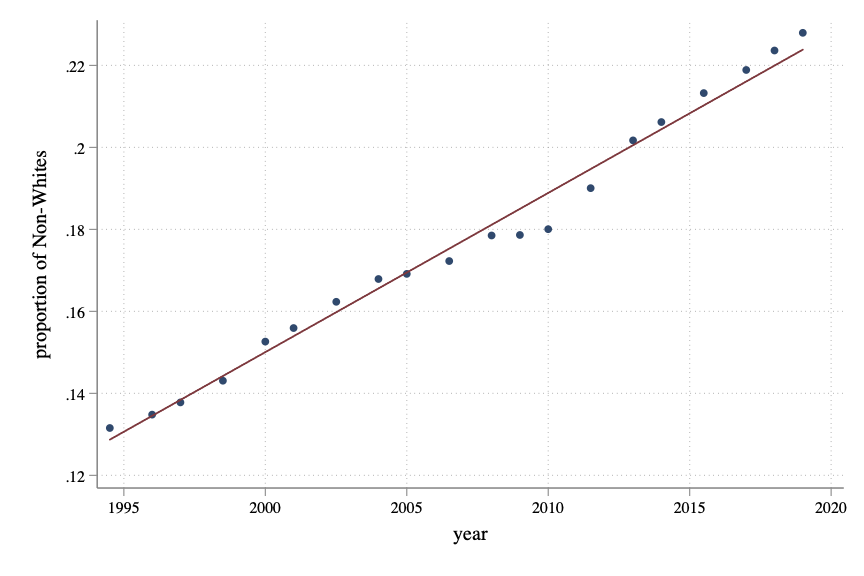
\includegraphics[width=\textwidth]{GraphNonWhites.png} 
\label{fig:1}
\end{center}
\end{figure}

\newpage

\begin{figure}[H]
\begin{center}
\caption{Hispanics as a percentage of the total population in the United States from 1995 to 2019.}
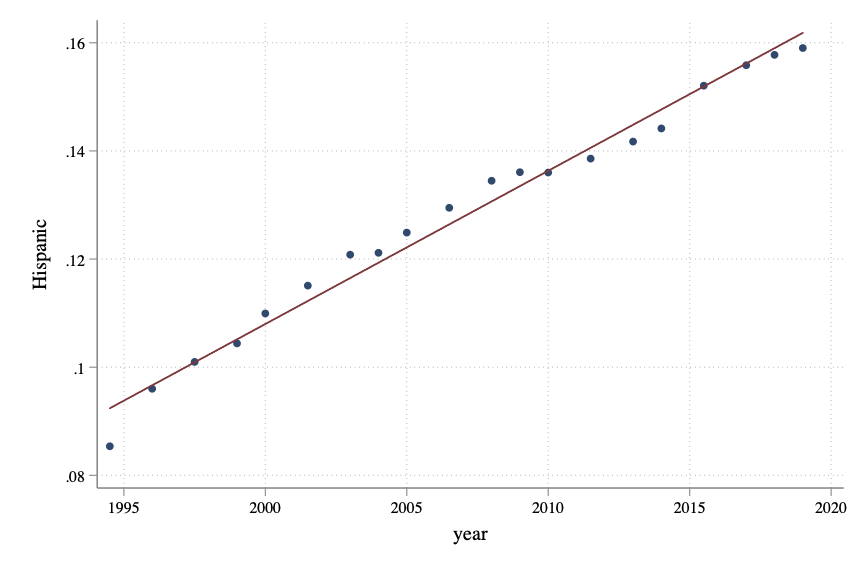
\includegraphics[width=\textwidth]{HispanicUSA.png} 
\label{fig:2}
\end{center}
\end{figure}

\newpage

\begin{figure}[H]
\begin{center}
\caption{Inter-racial marriages as a percent of all marriages \\
 in the United States from 1995 to 2020.}
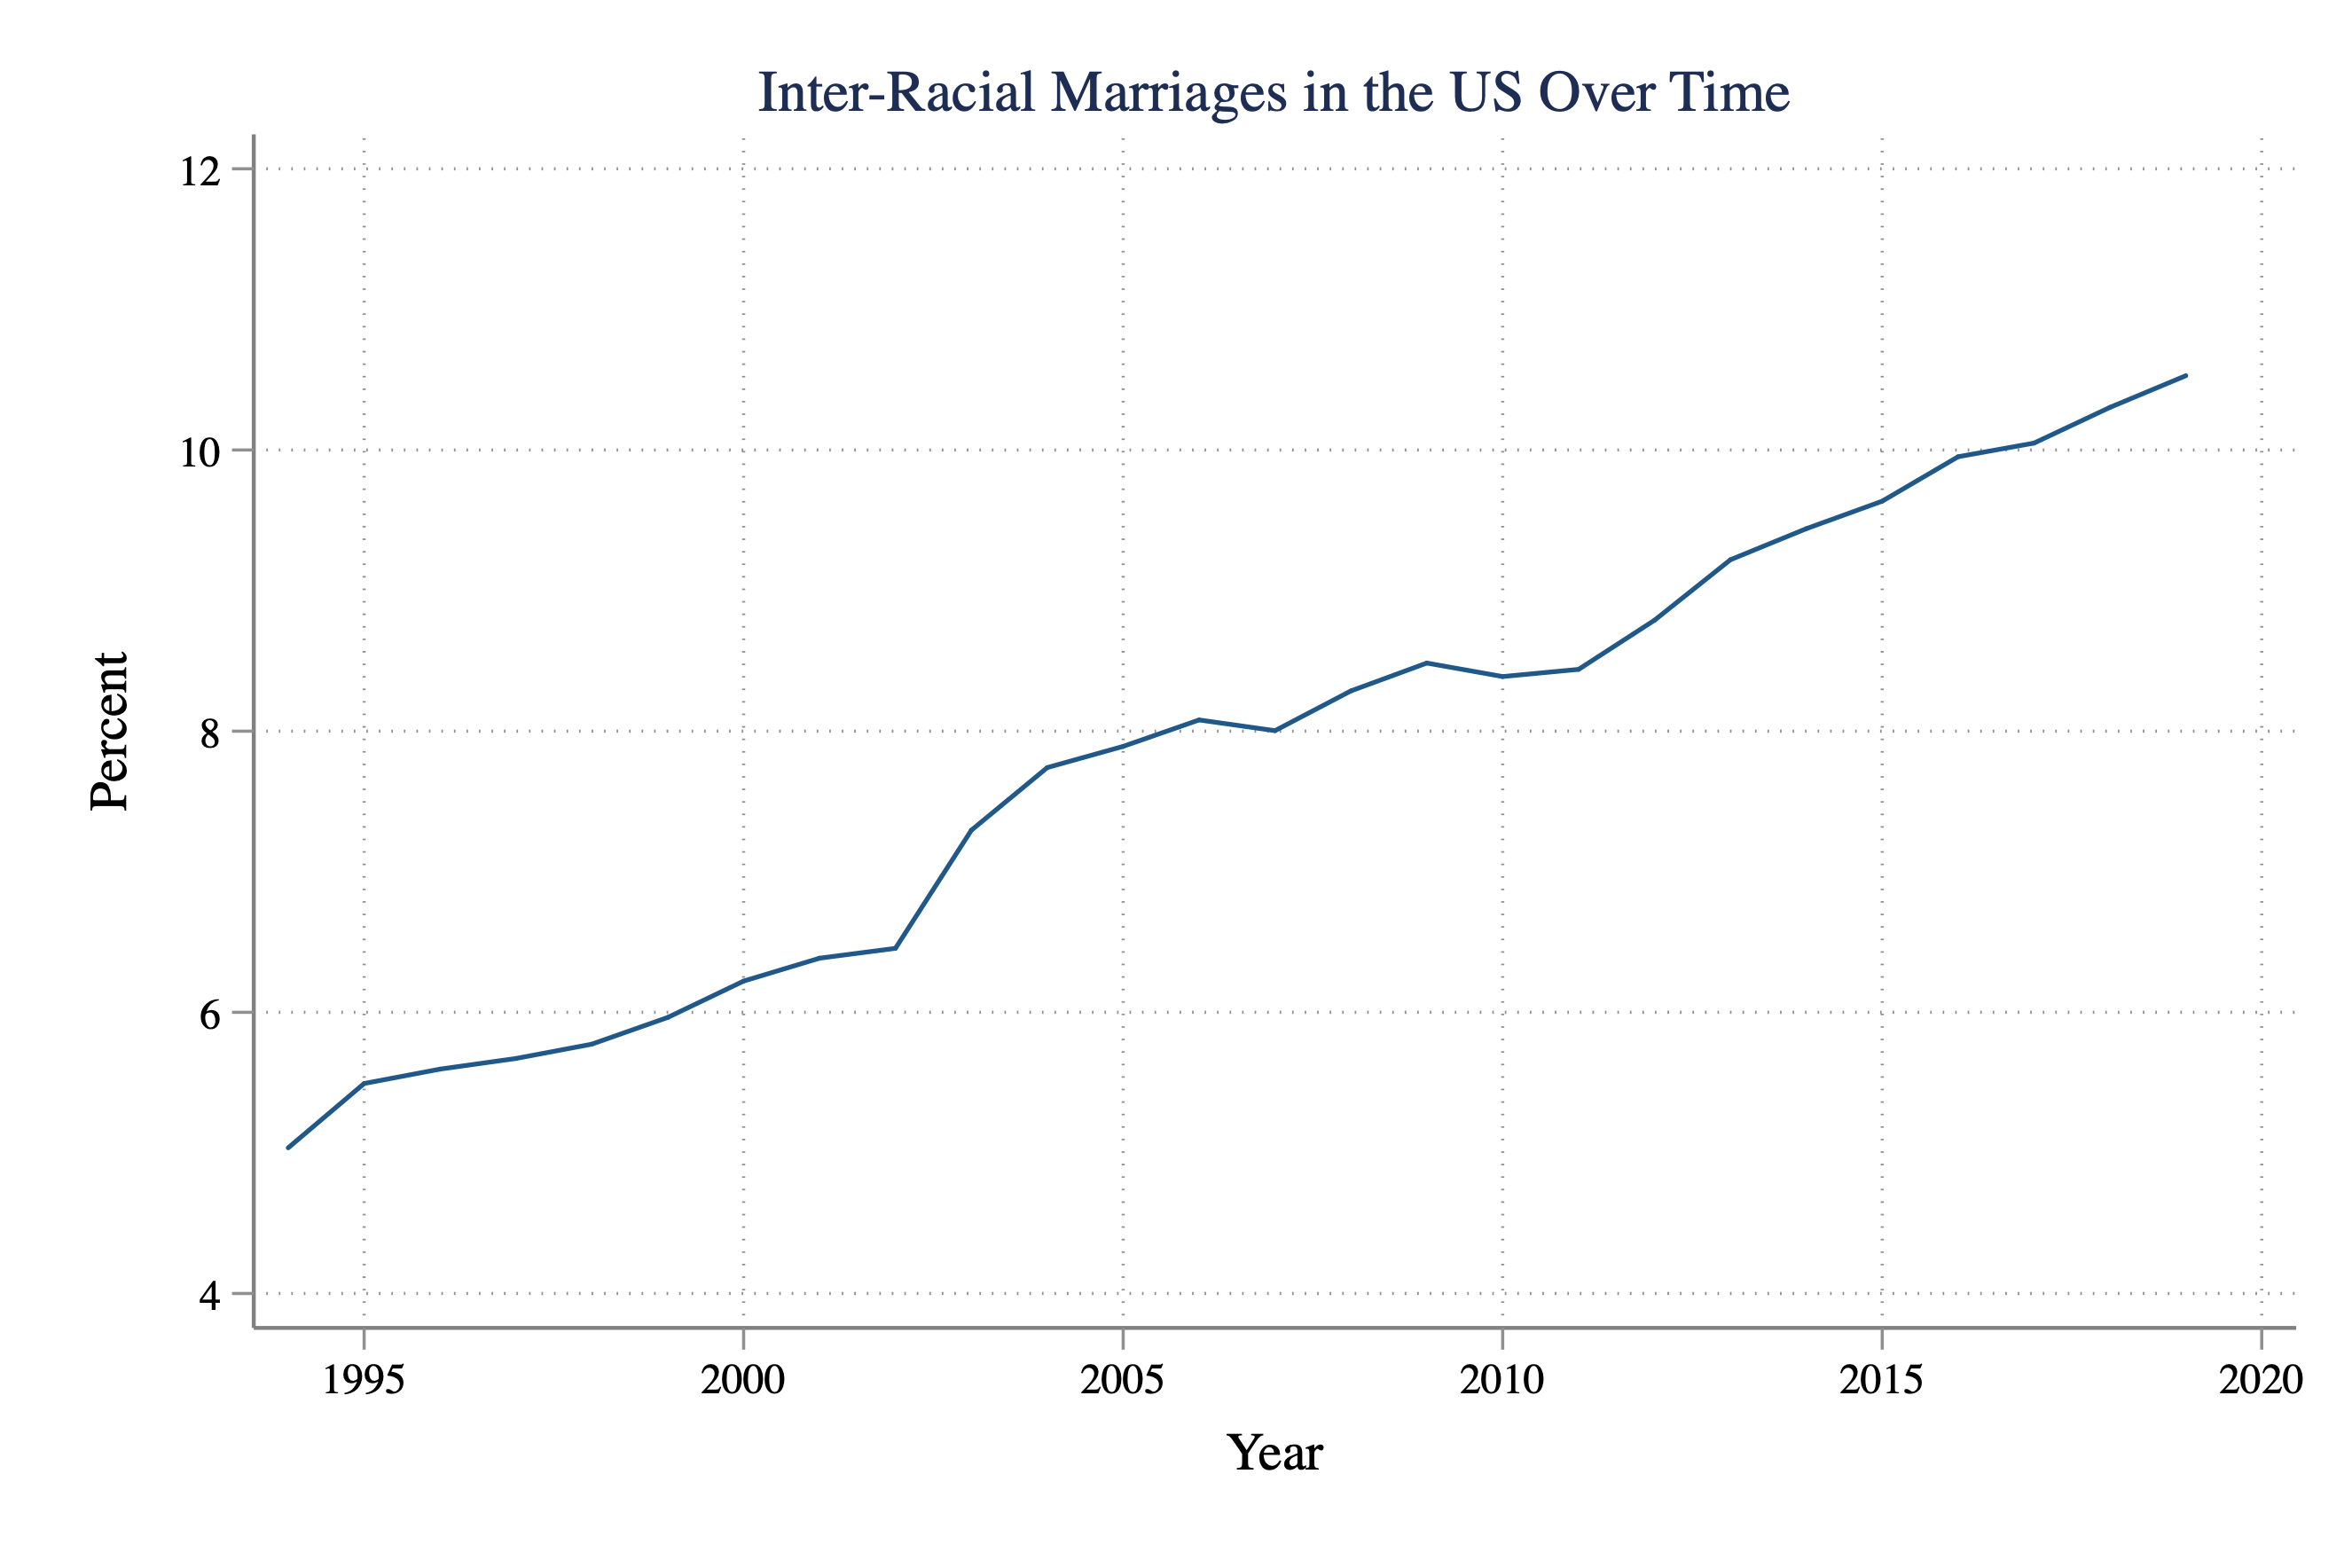
\includegraphics[width=\textwidth]{interracialovertime.png} 
\label{fig:3}
\end{center}
\end{figure}

\newpage

\begin{figure}[H]
\begin{center}
\caption{Distribution of the four types of children.}
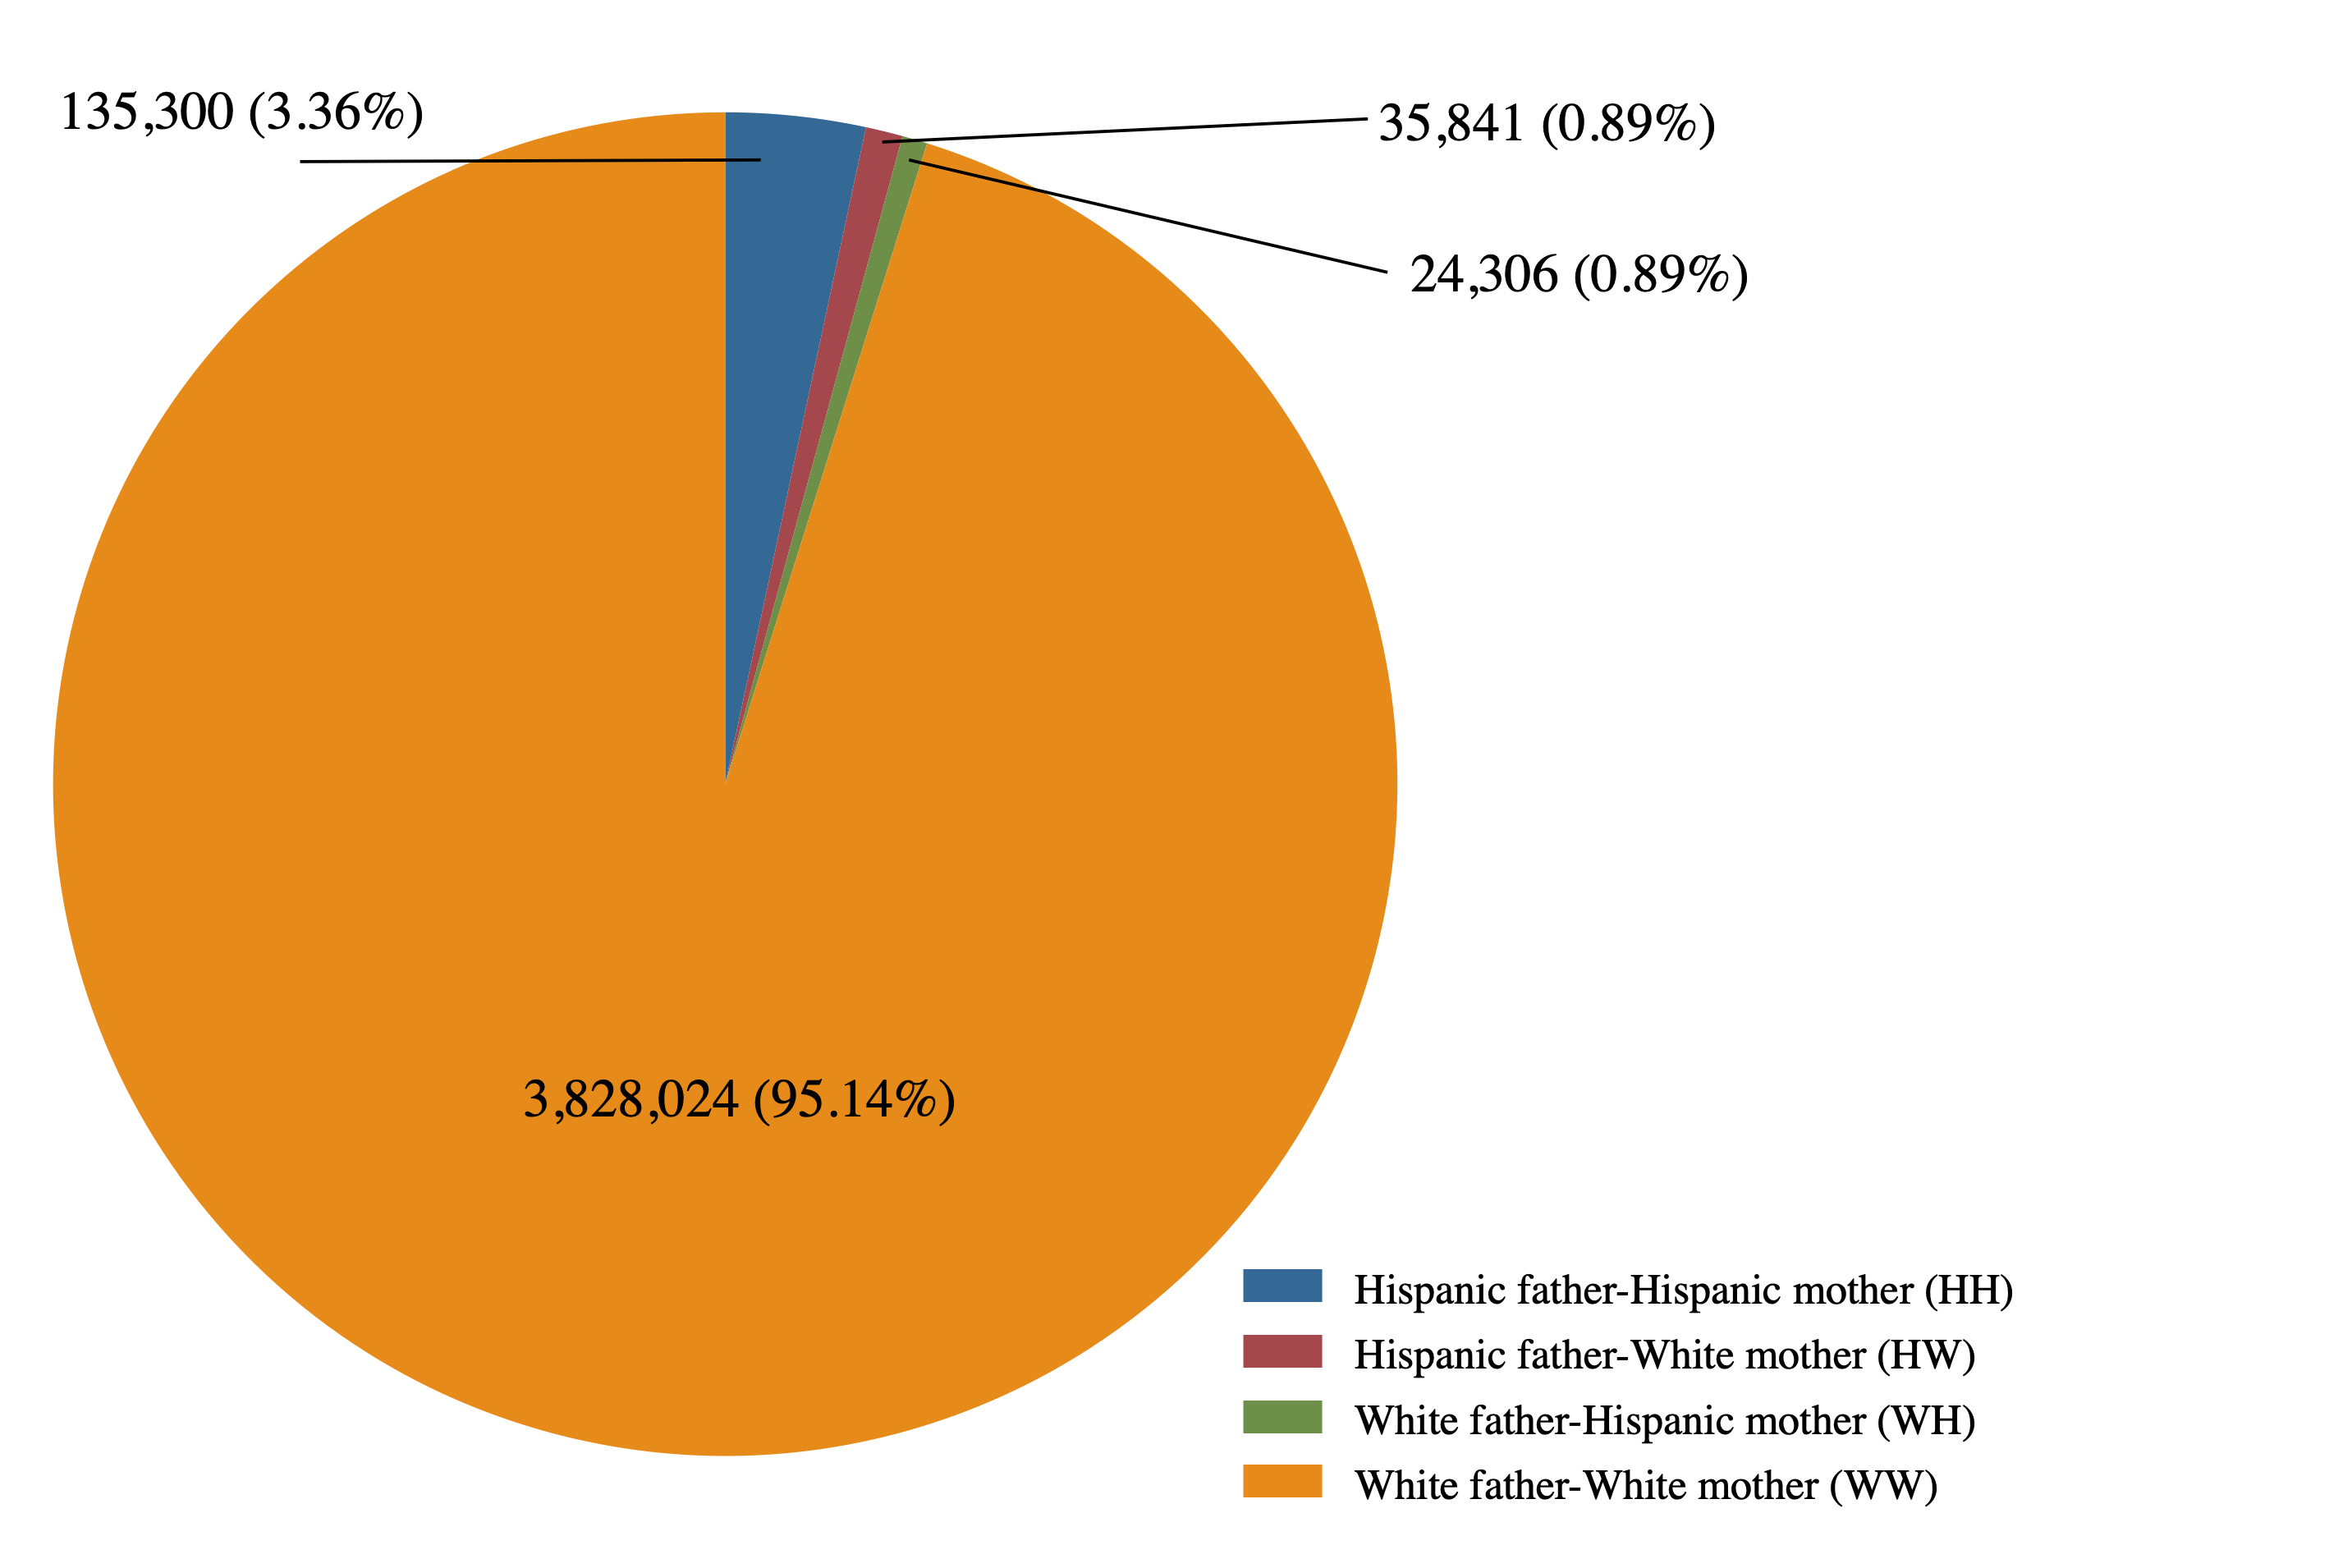
\includegraphics[width=\textwidth]{PirChart2.png} 
\label{fig:dist}
\end{center}
\end{figure}

\newpage
\begin{figure}[H]
\begin{center}
\caption{Chart explaining which synthetic parents and children \\
and when we observe them.}
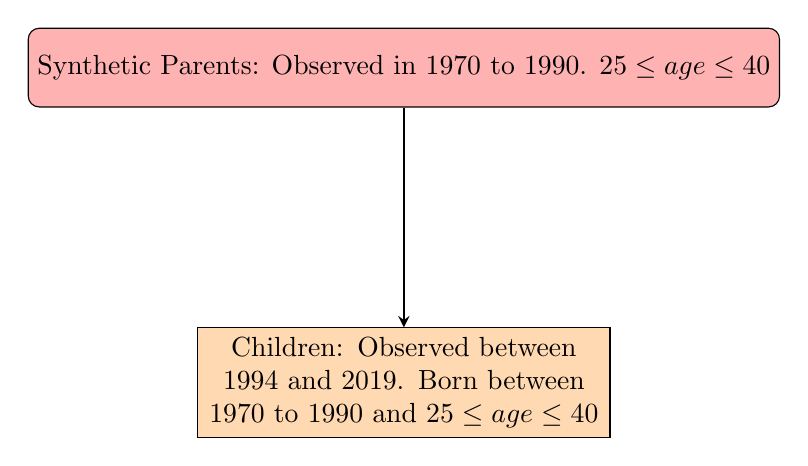
\begin{tikzpicture}[node distance =2cm]
\node (start) [startstop] {Synthetic Parents: Observed in 1970 to 1990. $25 \leq age \leq 40$};

\node (pro1) [process, below of = start, yshift = -2cm] {Children: Observed between 1994 and 2019. Born between 1970 to 1990 and $25 \leq age \leq 40$};

\draw [arrow] (start) -- (pro1);
\end{tikzpicture}
\label{flowchart1}
\end{center}
\end{figure}

\newpage

\begin{figure}[H]
\centering
\caption{Relationship Between Bias and Self-reported Identity on third-generation Hispanics: Interaction}
\label{fig:reg-interaction-third-by-num}
\begin{subfigure}{.48\textwidth}
\centering
\caption{Grandparents Combinations with One Objectively Hispanic Grandparent}
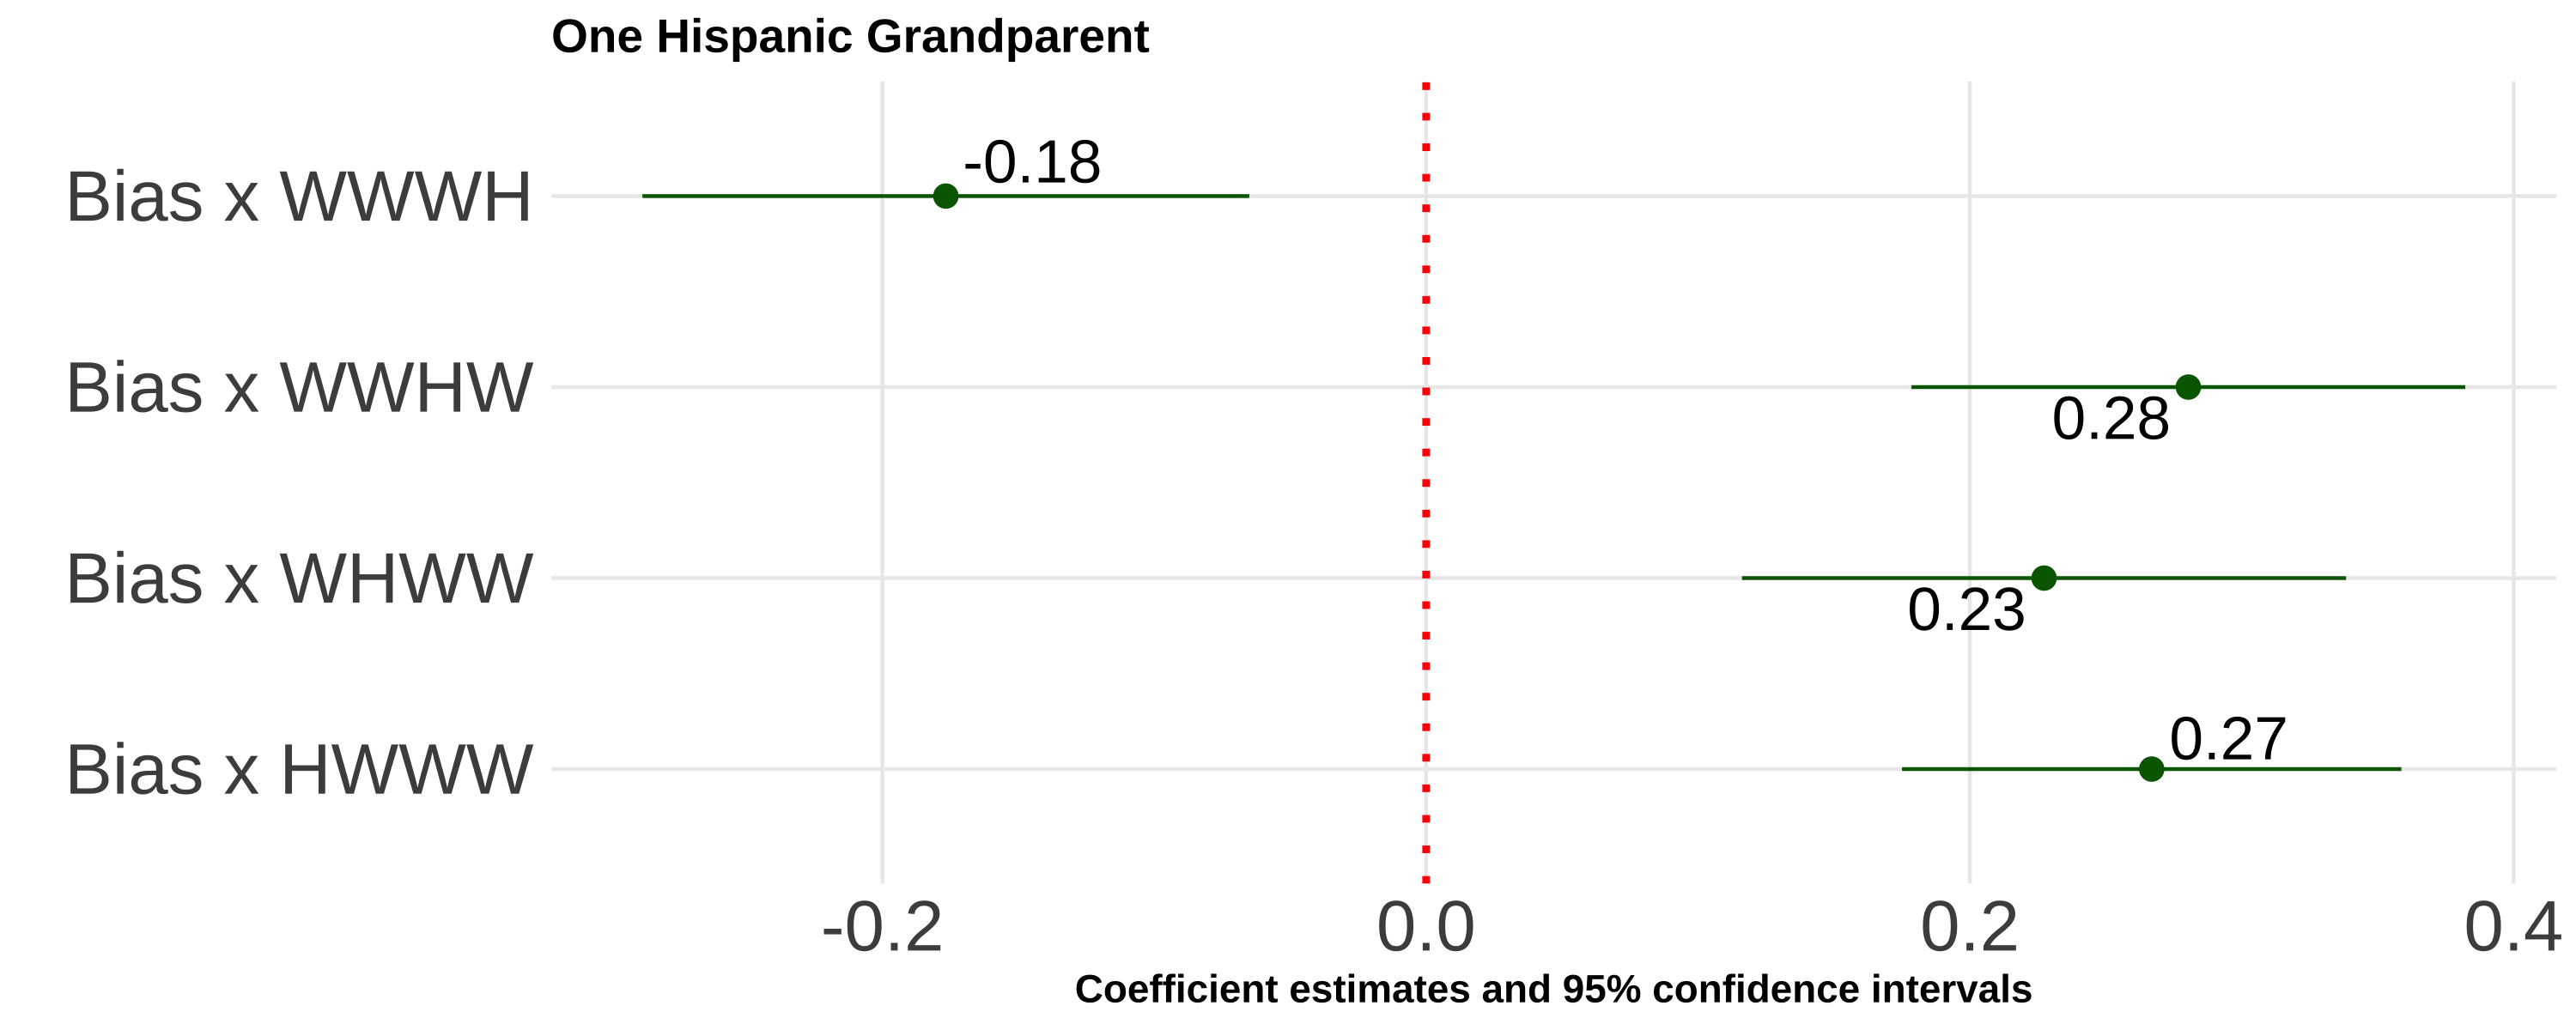
\includegraphics[width=.9\linewidth]{figure/skin-iat-regression-interaction-bygen-plot-one-hisp-grand.png}
\end{subfigure}
\centering
%Second graph
\begin{subfigure}{.48\textwidth}
\centering
\caption{Grandparents Combinations with Two Objectively Hispanic Grandparents}
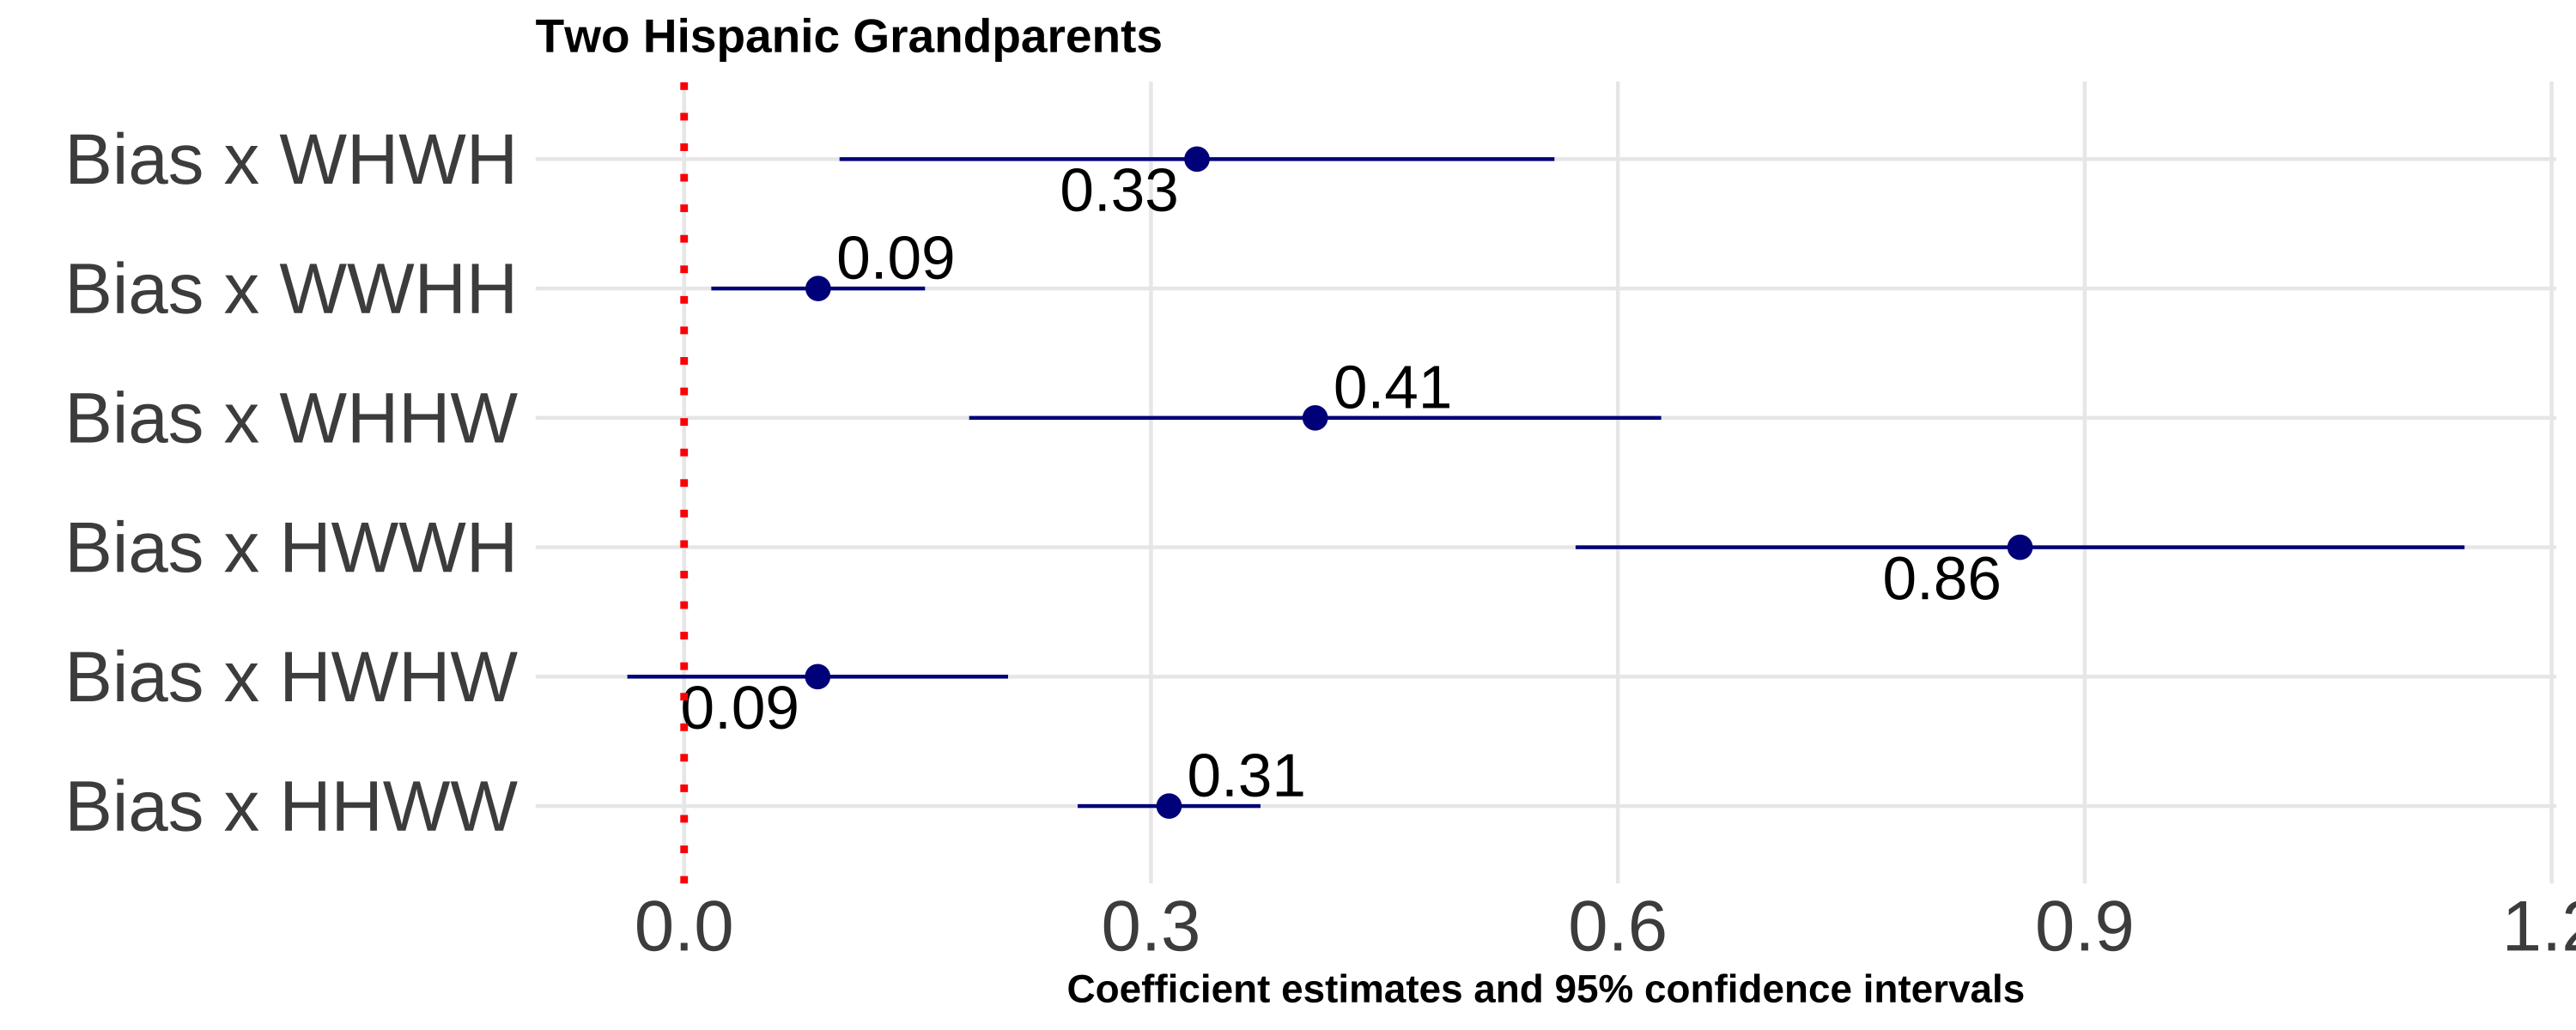
\includegraphics[width=.9\linewidth]{figure/skin-iat-regression-interaction-bygen-plot-two-hisp-grand.png}
\end{subfigure}
%Third
\begin{subfigure}{.48\textwidth}
\centering
\caption{Grandparents Combinations with Three Objectively Hispanic Grandparents}
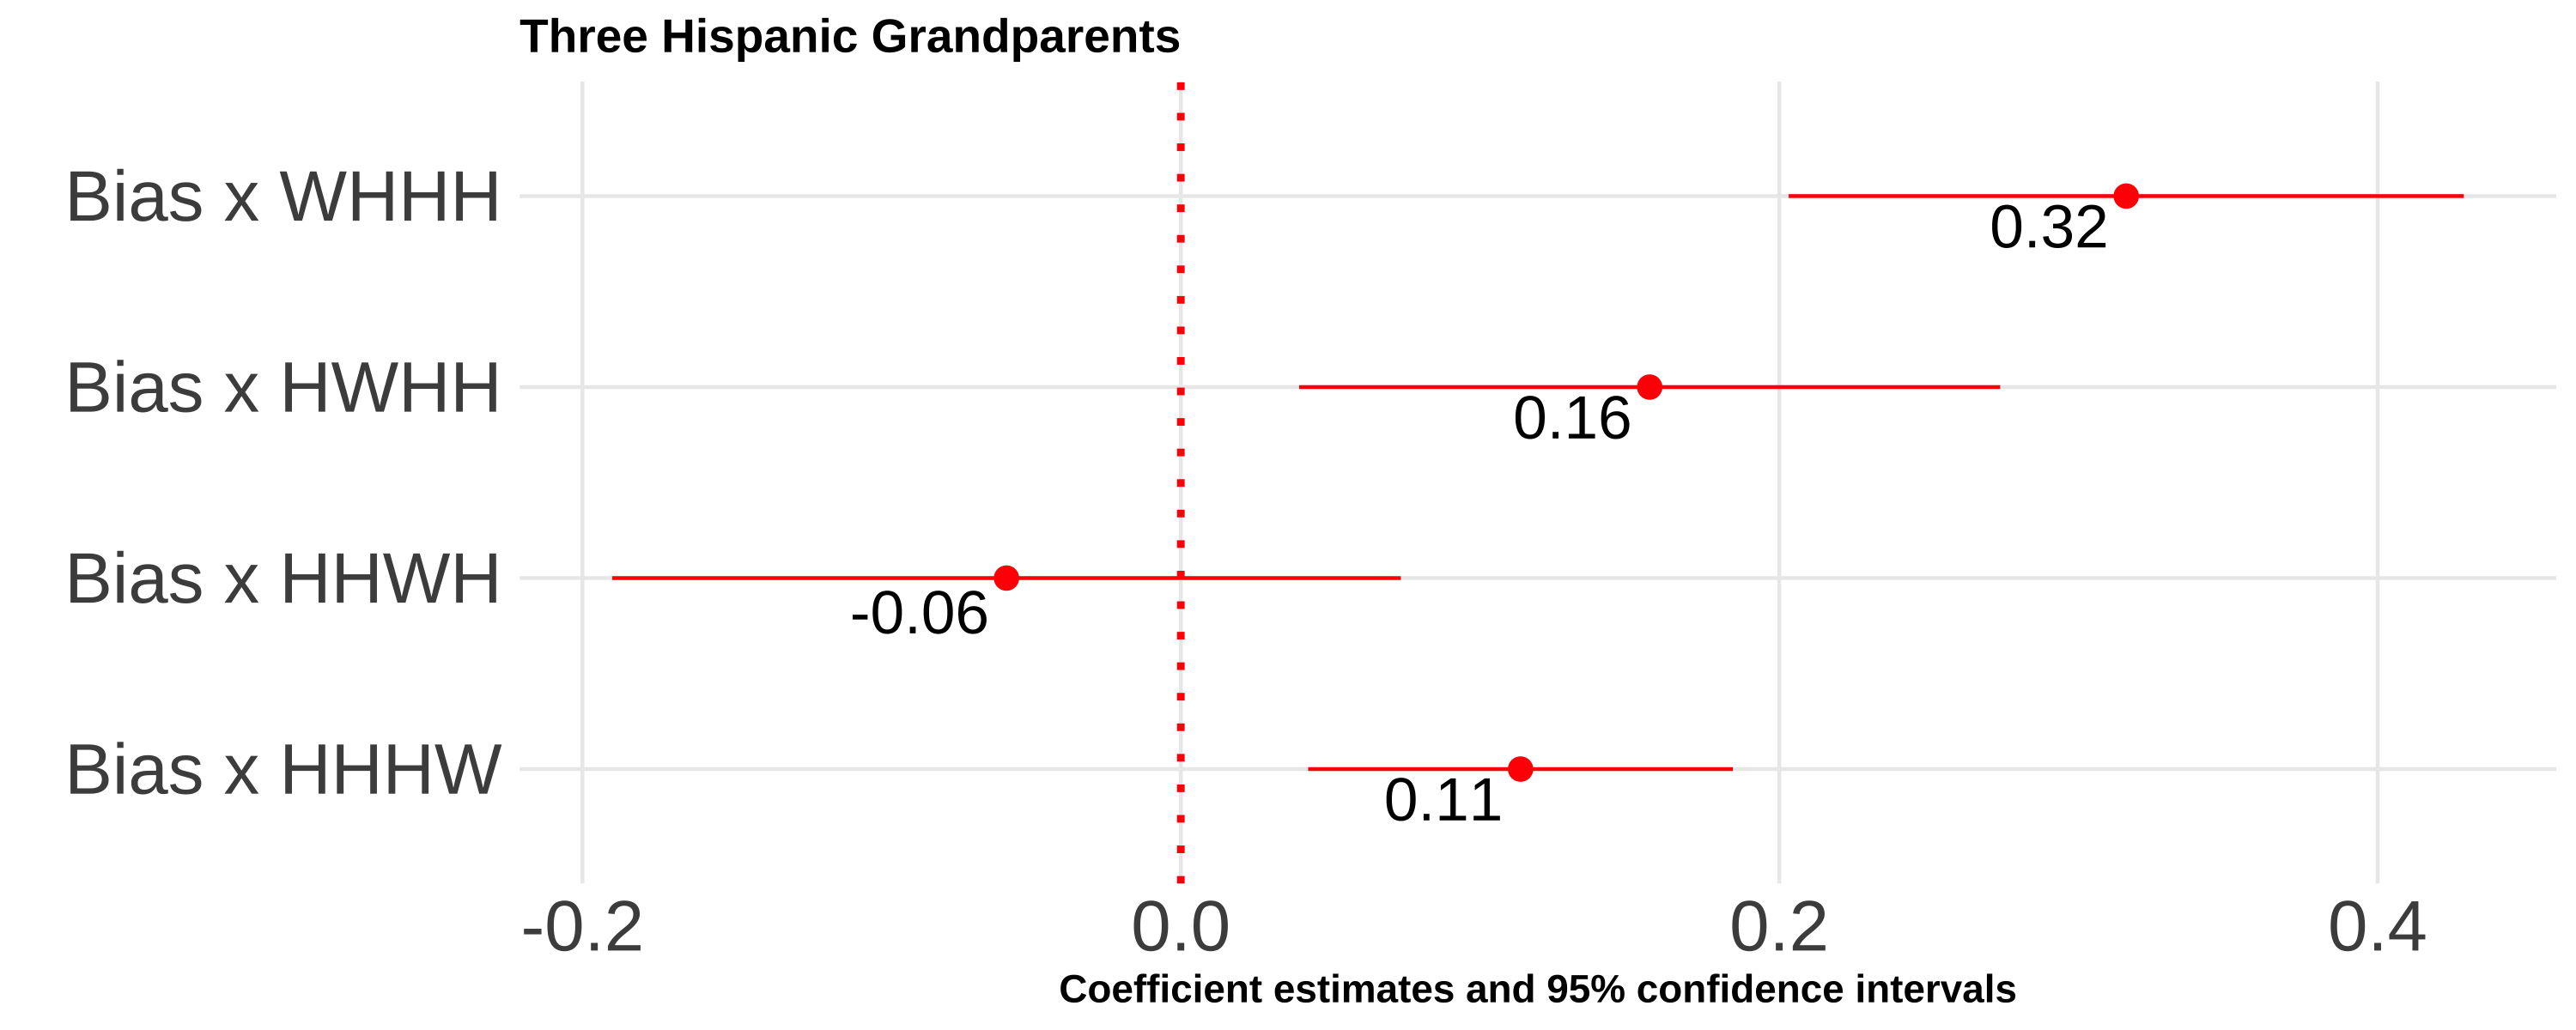
\includegraphics[width=.9\linewidth]{figure/skin-iat-regression-interaction-bygen-plot-three-hisp-grand.png}
\end{subfigure}

\flushleft\footnotesize{\note{I show four panels of estimating equation (\ref{eq:identity_reg_bias_interaction_3}). I include region $\times$ year fixed effects with controls for sex, quartic age, and parental education. Each panel results from the same regression but of a different combination of grandparents types. Robust standard errors are reported. The samples include third-generation Hispanic children ages 17 and below who live in intact families. Third-generation Hispanic immigrant children with native-born parents and at least one grandparent born in a Spanish-speaking country.}}
\end{figure}

\pagebreak
\newpage


\begin{figure}[H]
\centering
\caption{Scatter Plot of Proportion Subjectively Hispanic on Bias}
\label{scatter-plot-1}
\begin{subfigure}{.9\textwidth}
\caption{Year < 2015}
\centering
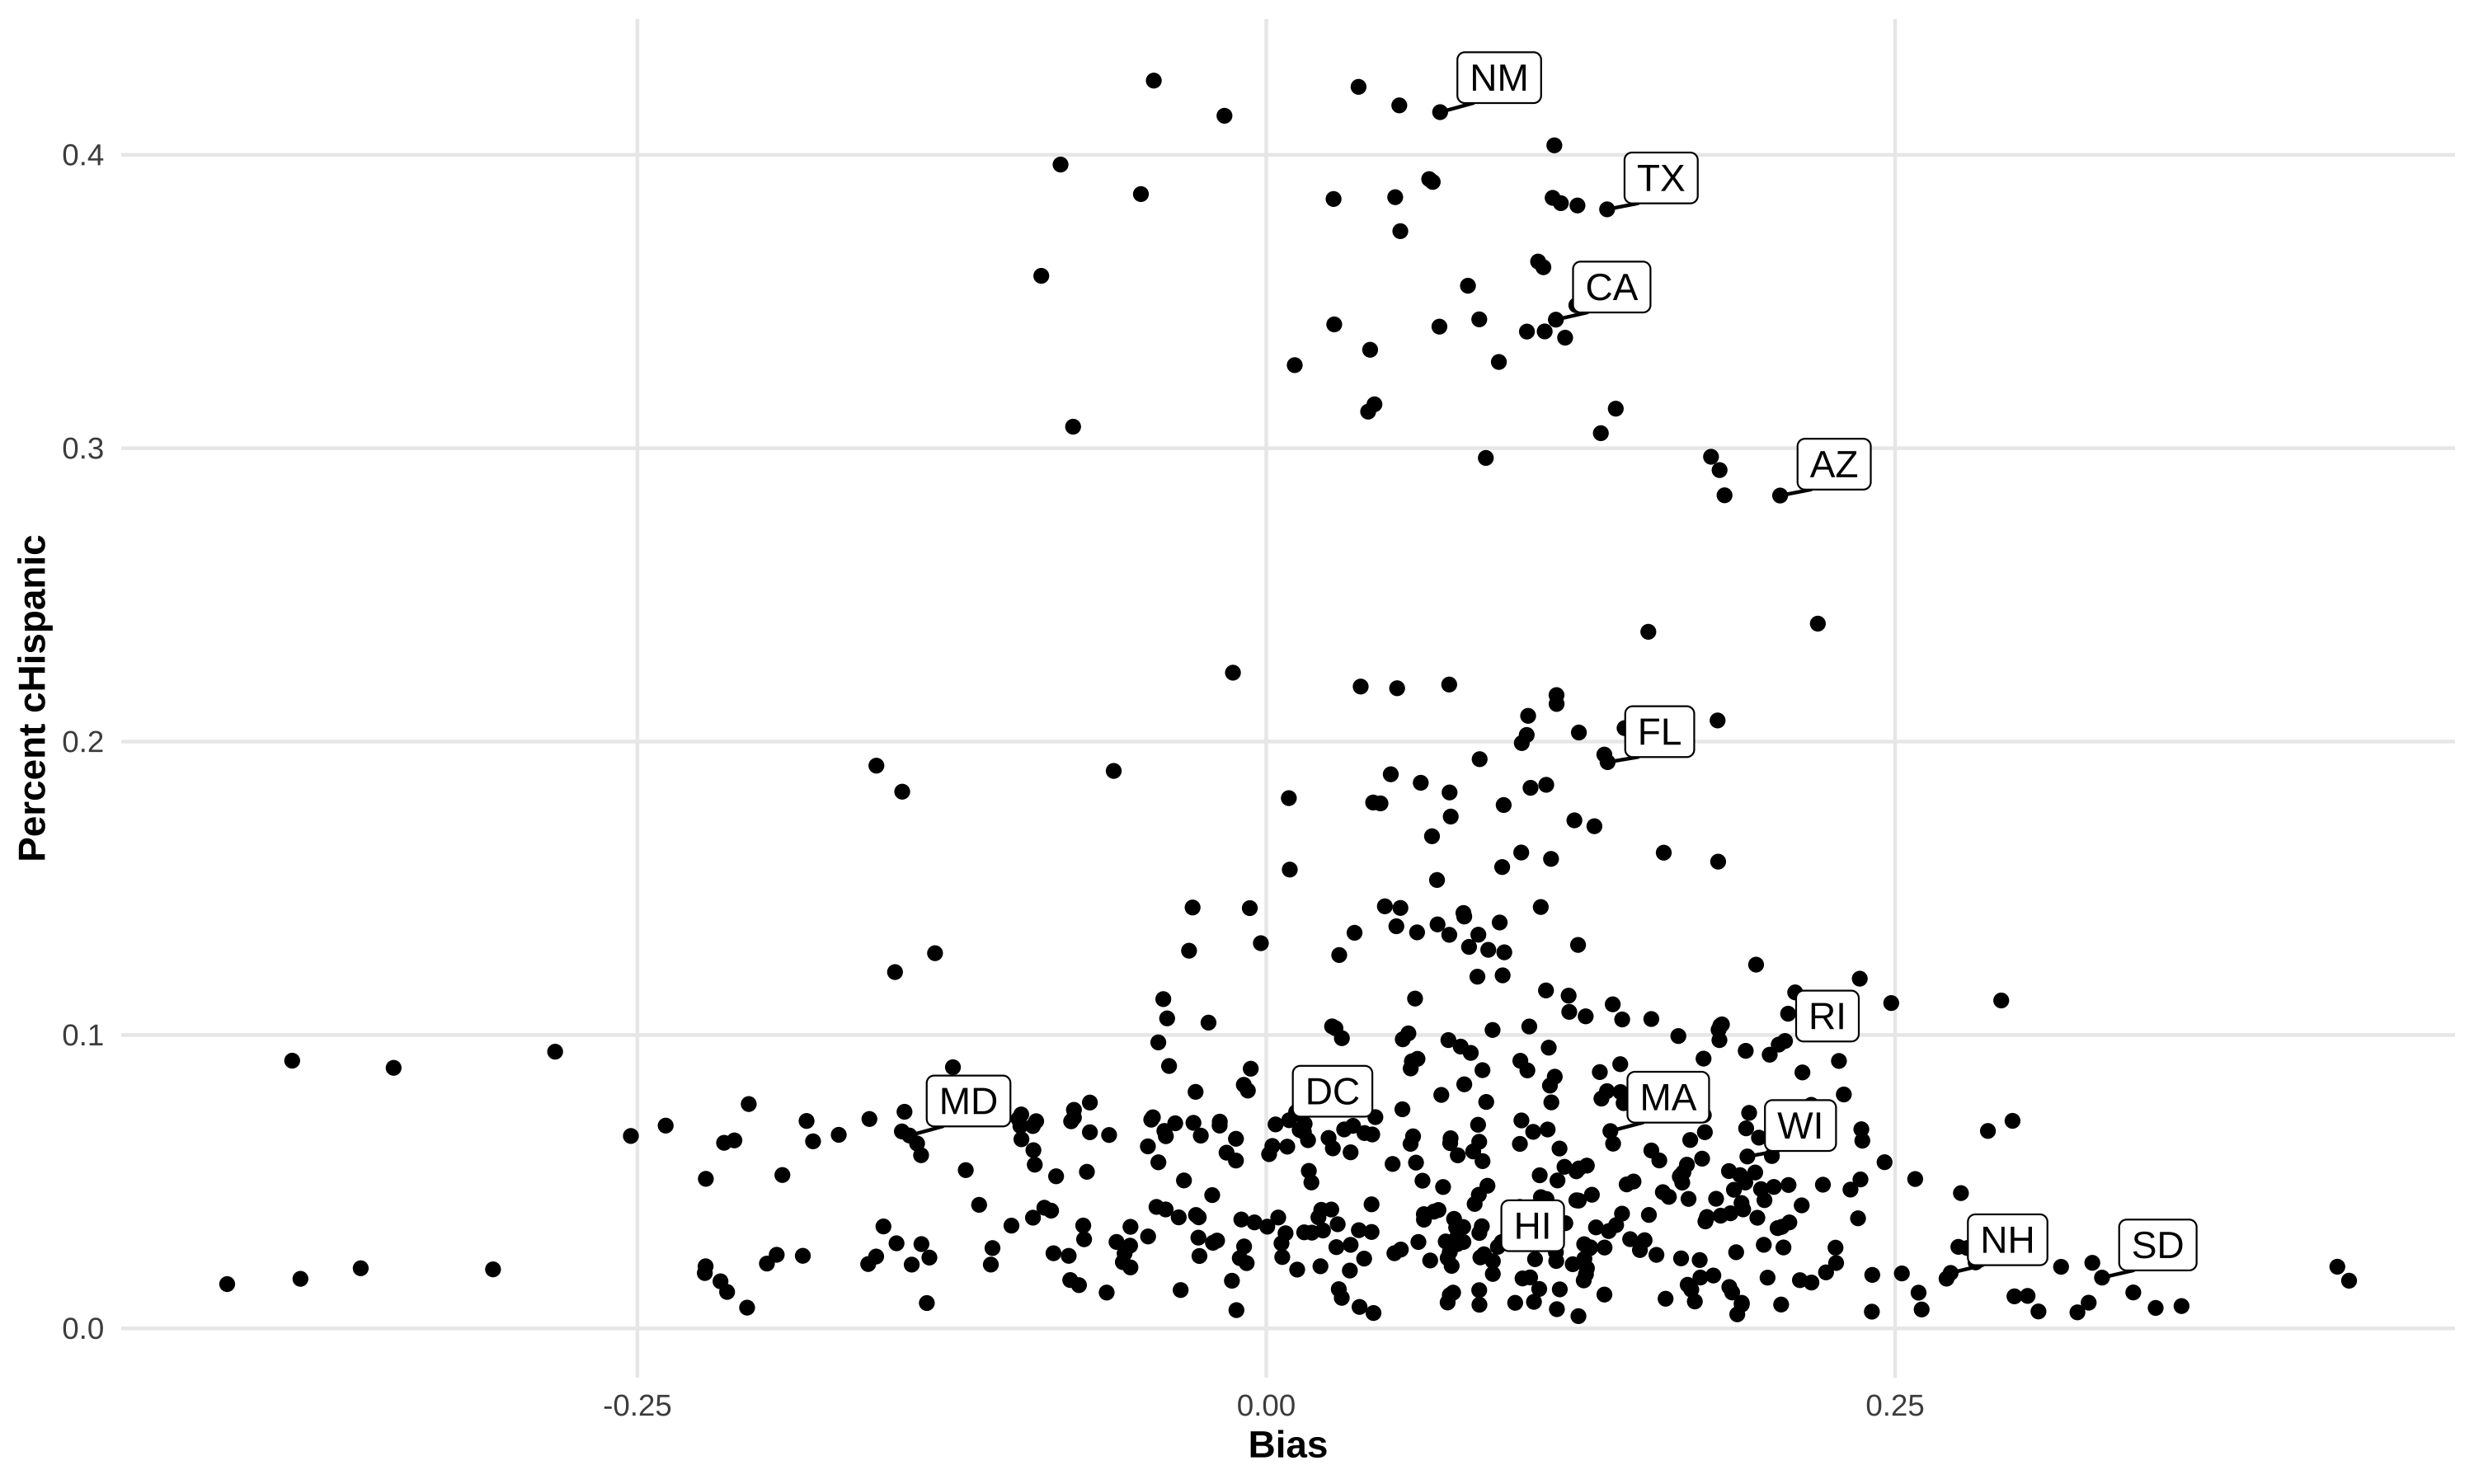
\includegraphics[width=.9\linewidth]{figure/scatter-plot-bias-hispanic-less2015.png}
\end{subfigure}
\centering
%Second graph
\begin{subfigure}{.9\textwidth}
\caption{Year $\geq$ 2015}
\centering
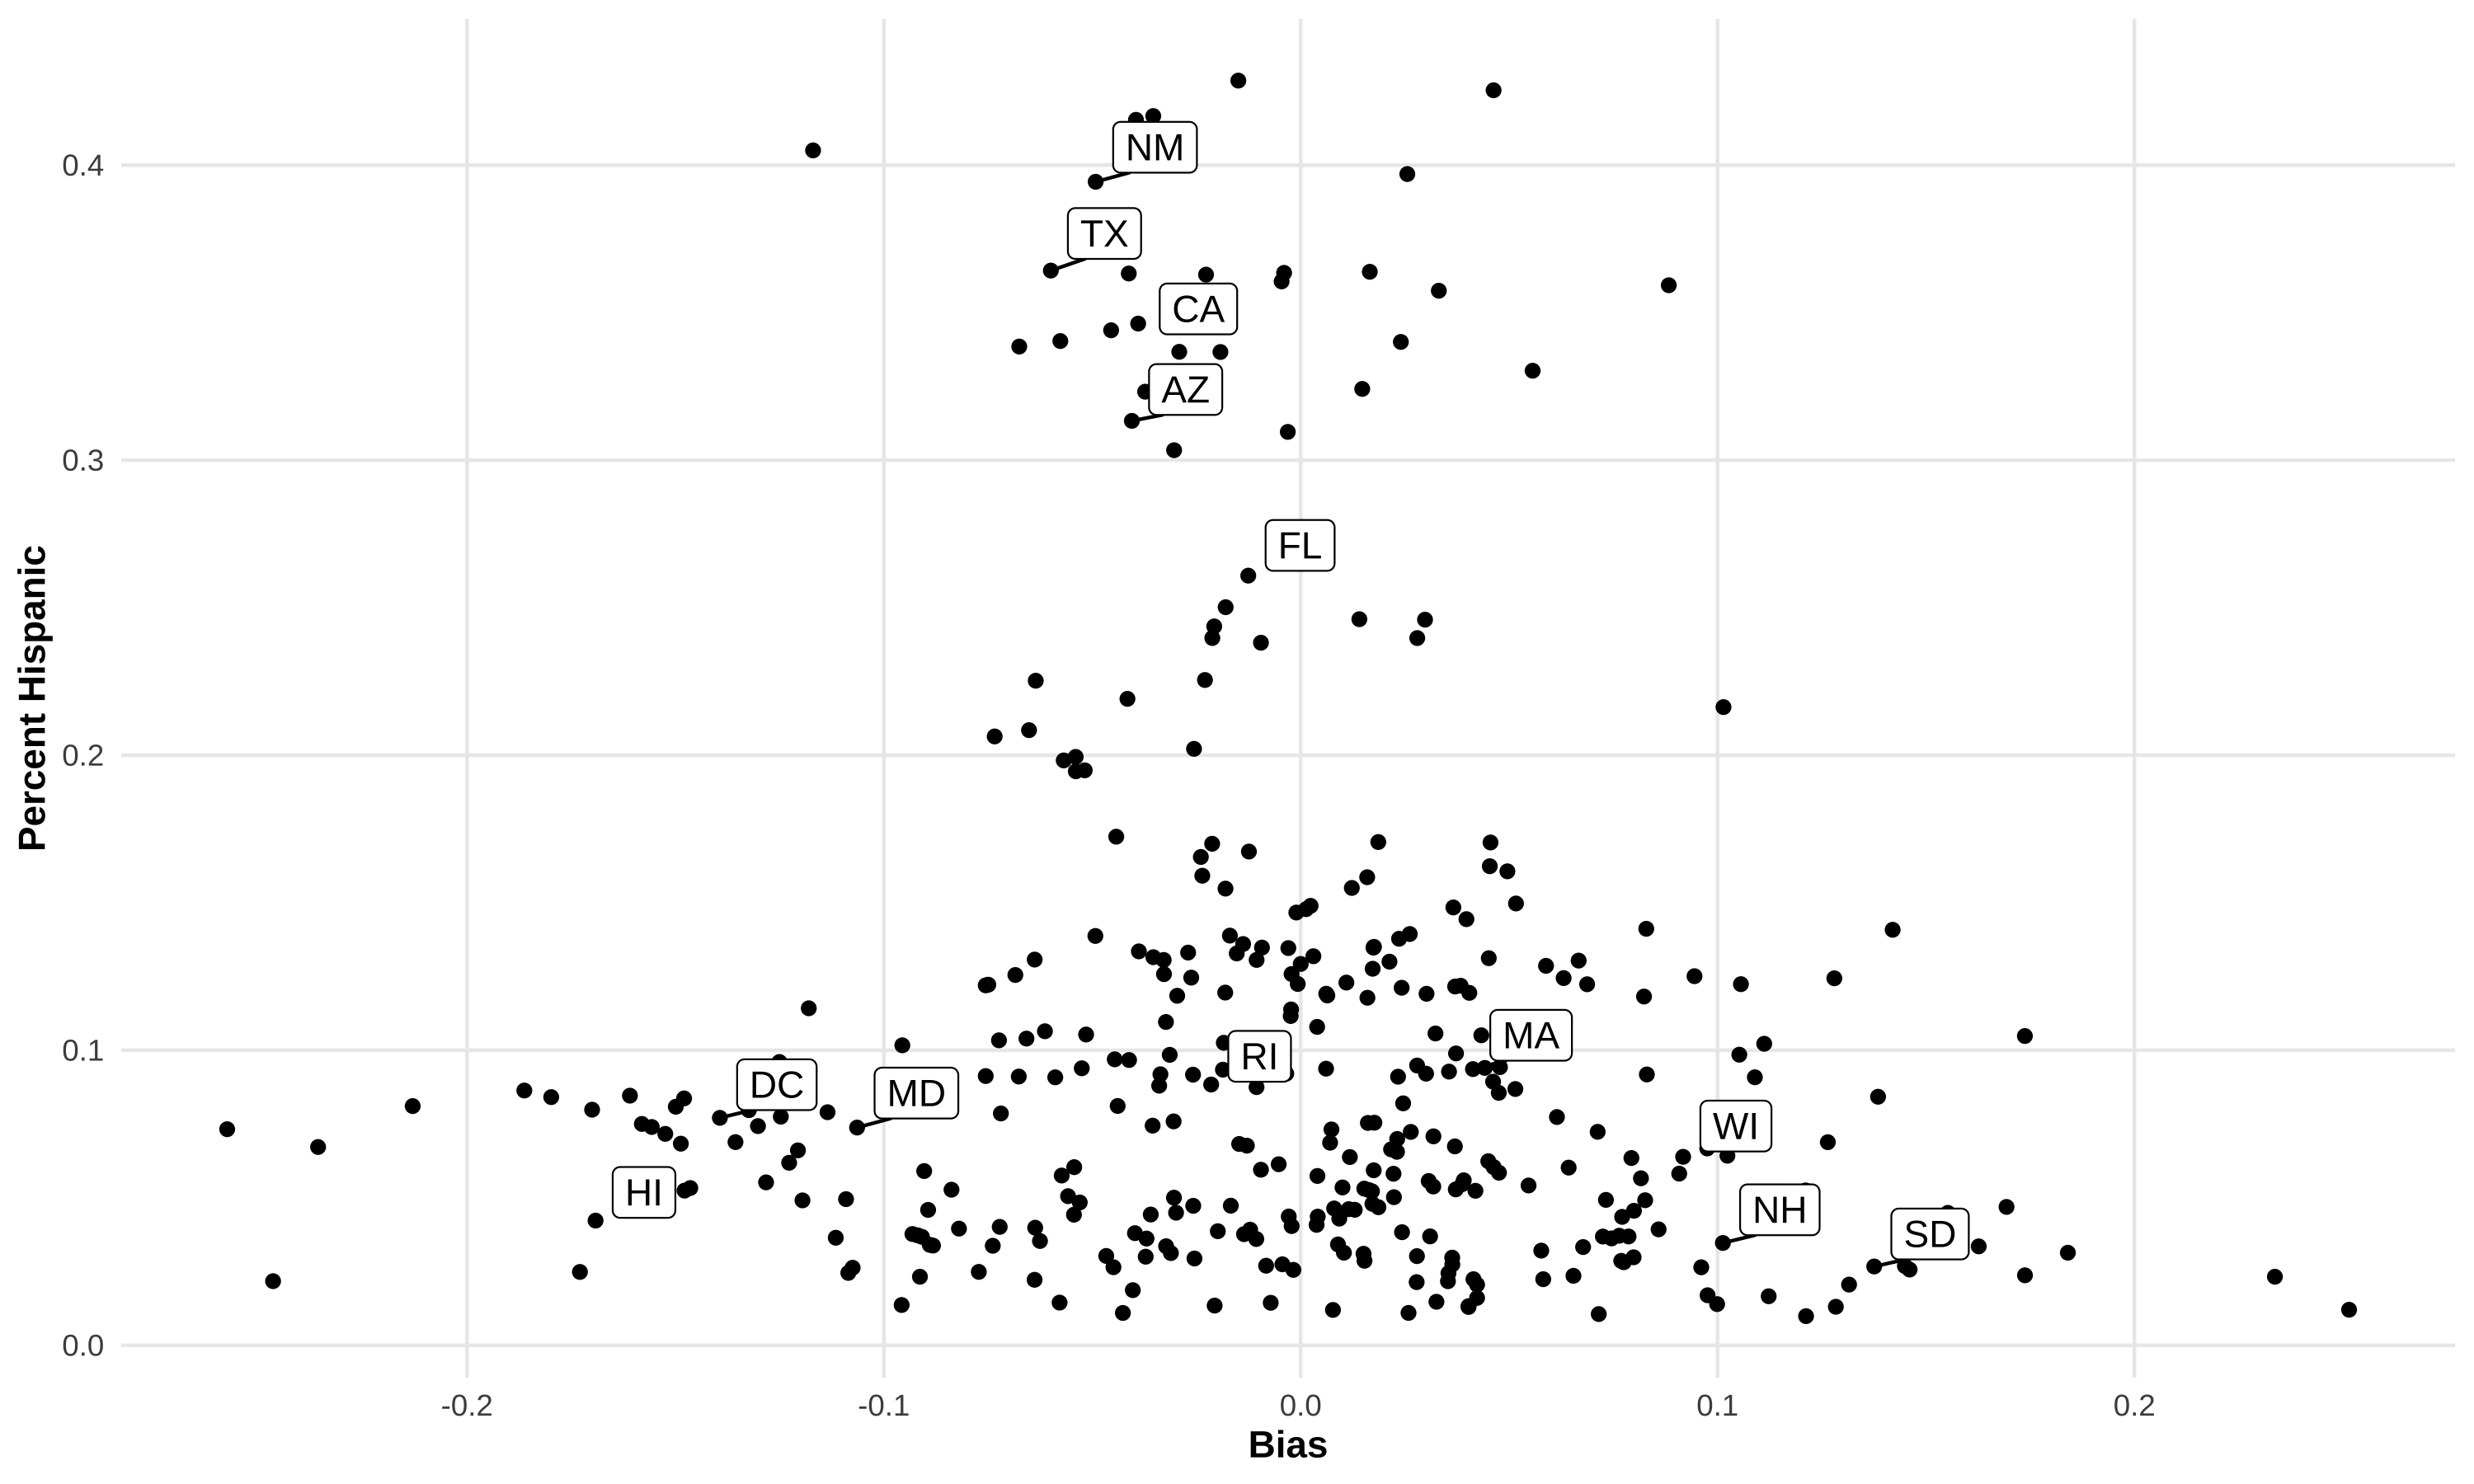
\includegraphics[width=.9\linewidth]{figure/scatter-plot-bias-hispanic-great2015.png}
\end{subfigure}
\flushleft\footnotesize{\note{Here are two scatter plots of bias on subjective Hispanic population in a state. Each dot represents a state in a certain year. Percent subjectively Hispanic = $\frac{\# \text{Hispanics}}{\text{Population}}$ \\
\emph{Source.} 2004-2021 Current Population Survey and 2004-2021 Implicit Association Test as a proxy for bias.}}
\end{figure}

\newpage
\pagebreak

\begin{figure}[H]
\centering
\caption{Scatter Plot of Proportion Second-Generation and Both Parents Born in a Spanish-Speaking Country on Bias}
\label{scatter-plot-4}
\begin{subfigure}{.9\textwidth}
\caption{Year < 2015}
\centering
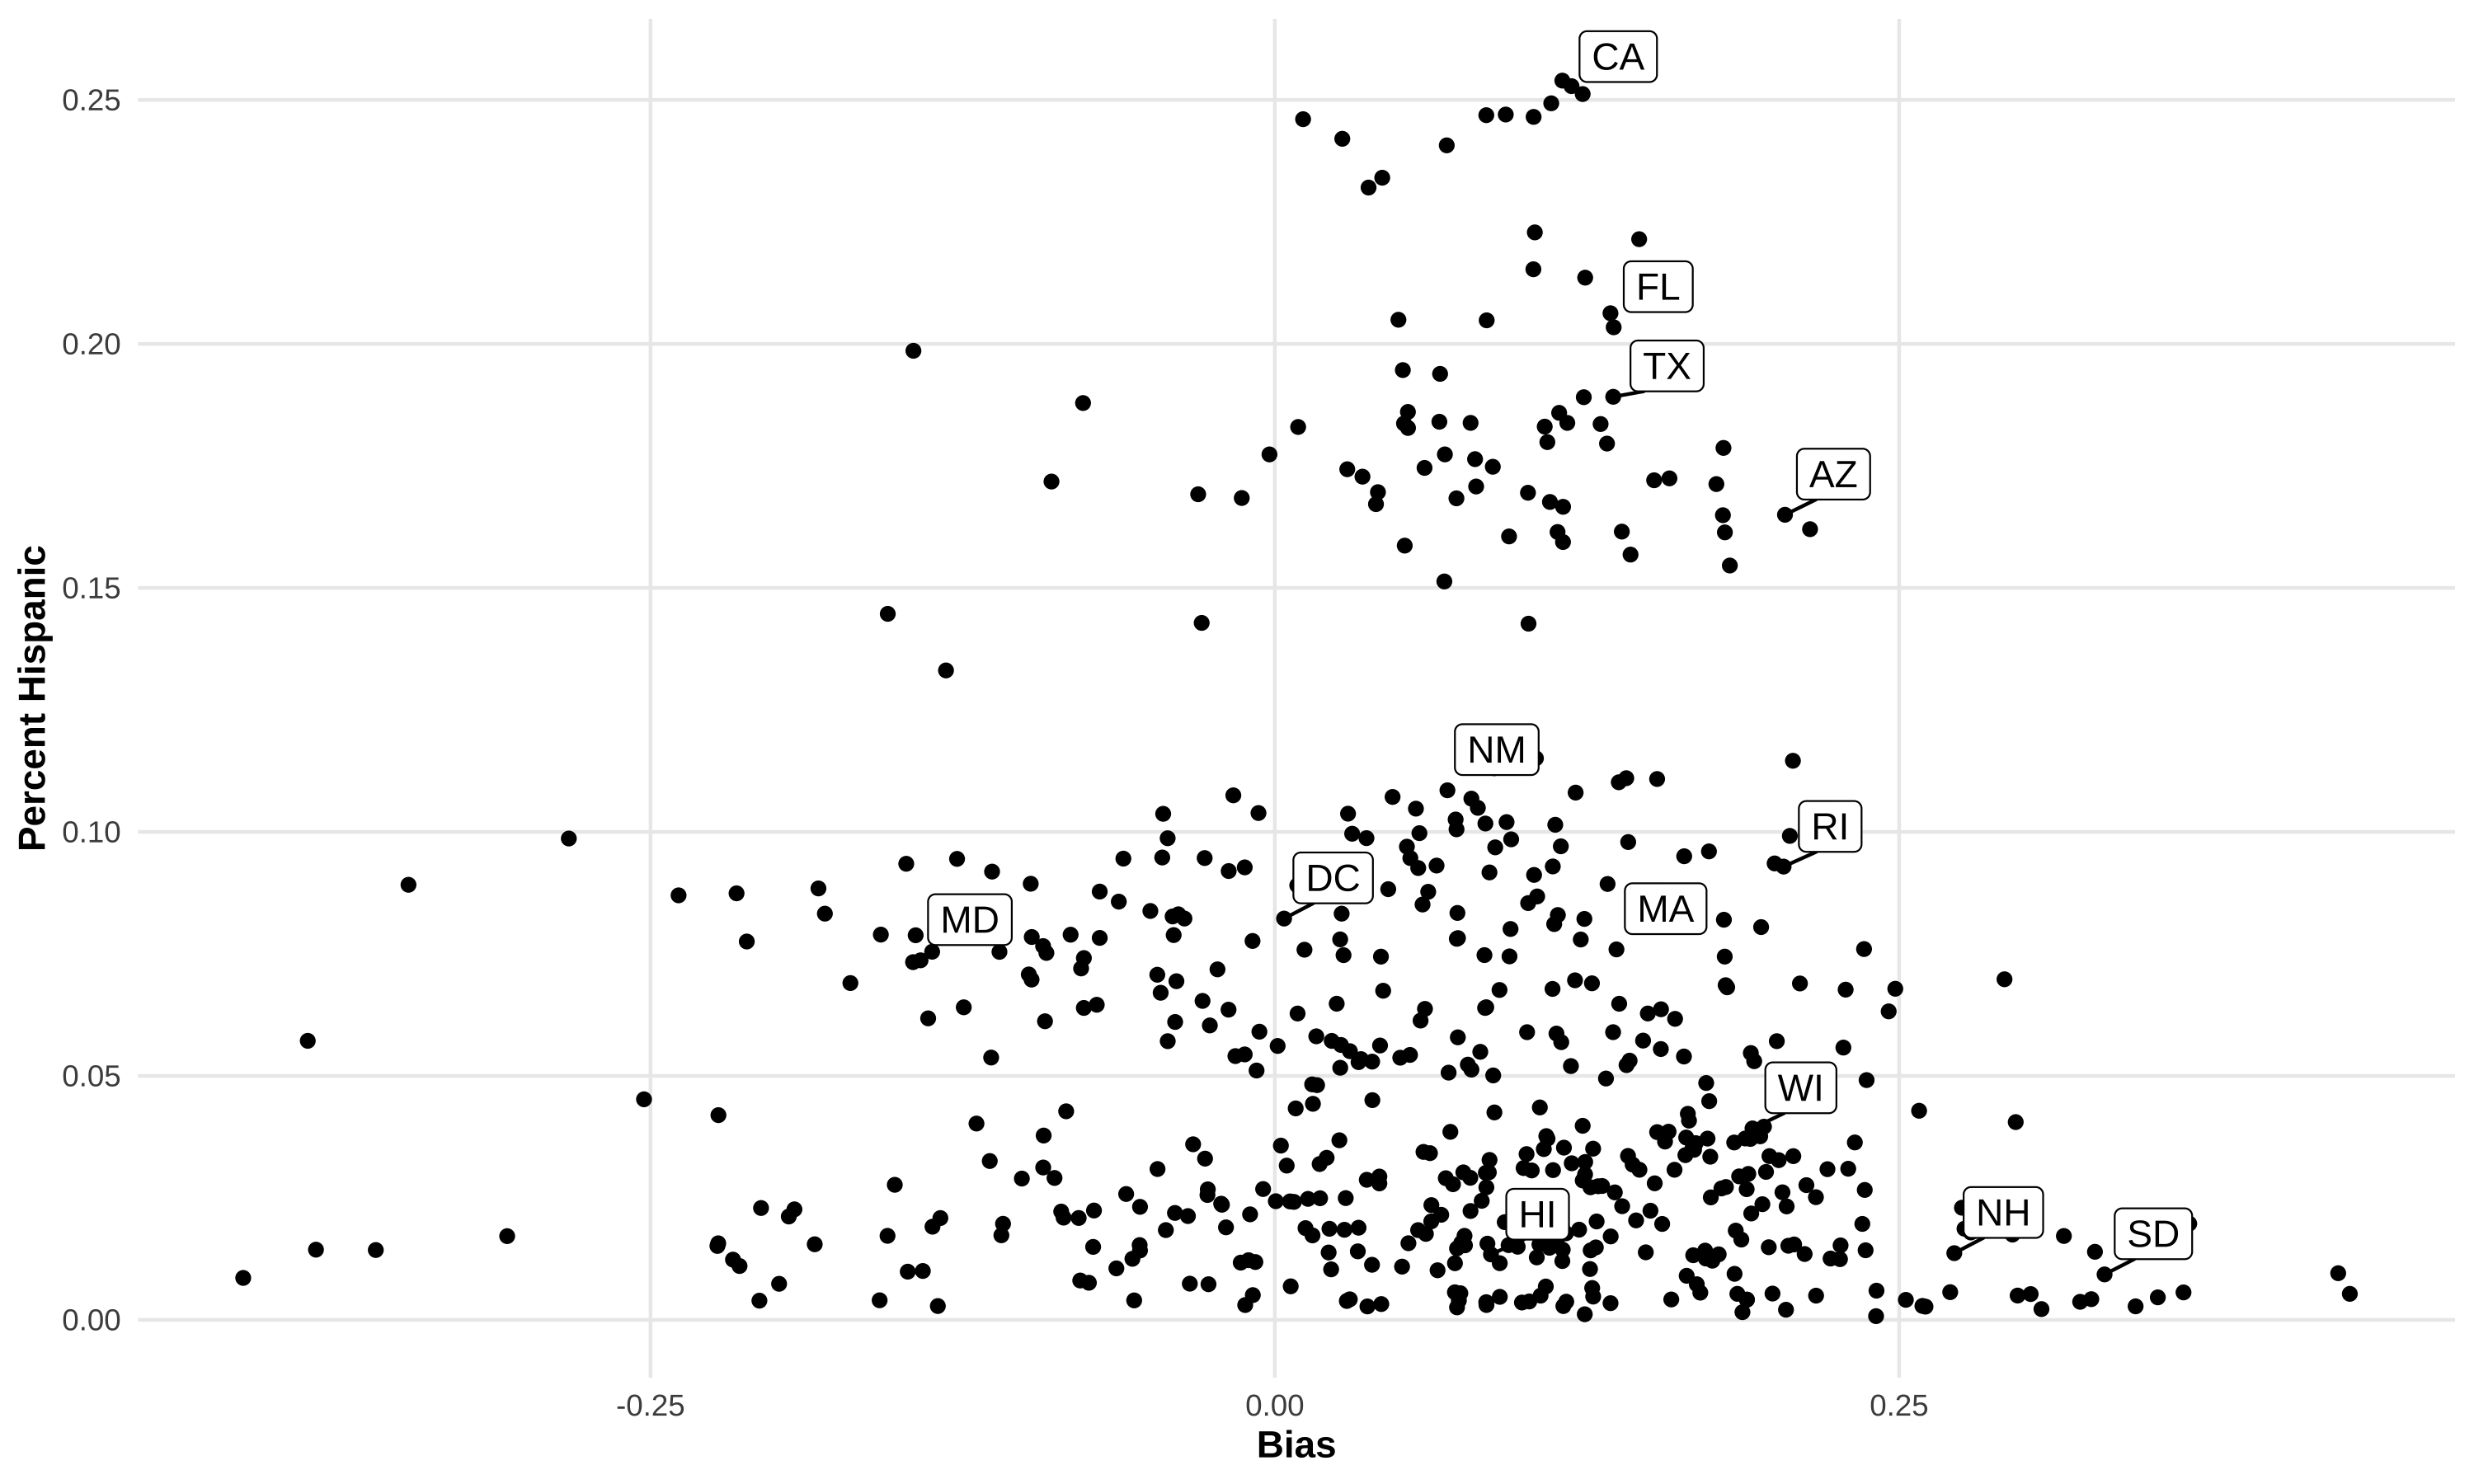
\includegraphics[width=.9\linewidth]{figure/scatter-plot-bias-hh-hispanic-less2015-hh.png}
\end{subfigure}
\centering
%Second graph
\begin{subfigure}{.9\textwidth}
\caption{Year $\geq$ 2015}
\centering
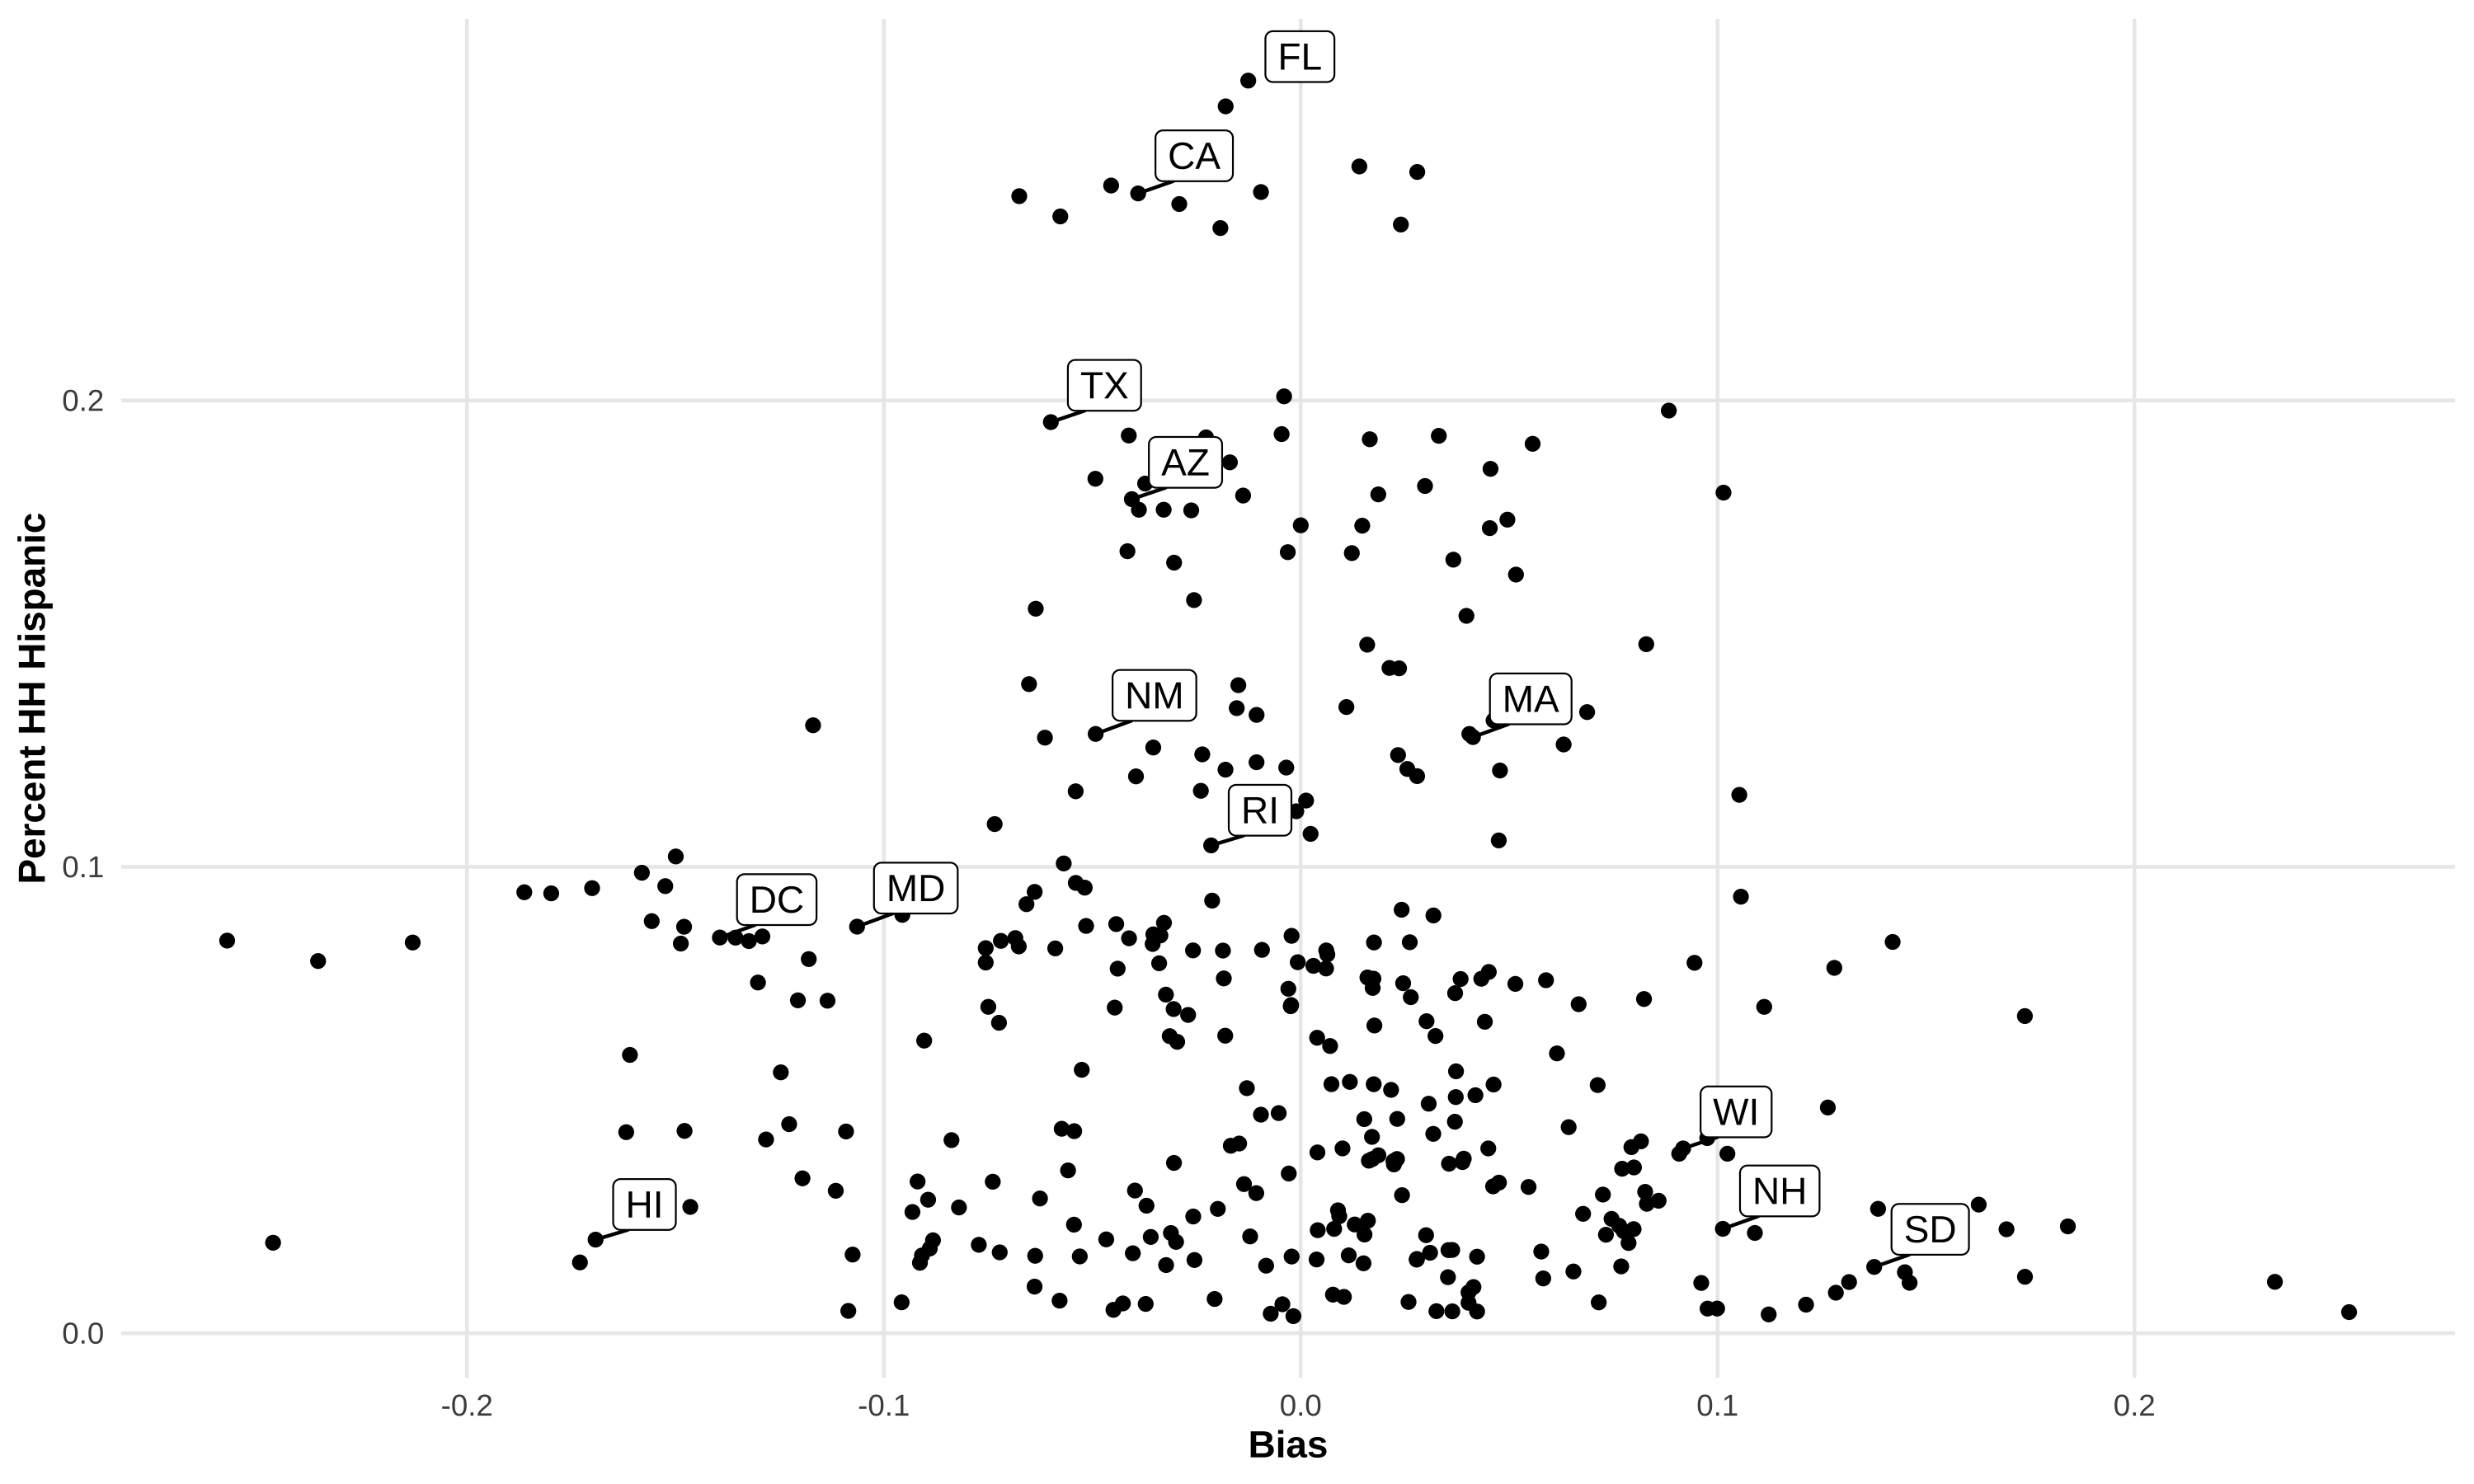
\includegraphics[width=.9\linewidth]{figure/scatter-plot-bias-hh-hispanic-great2015-hh.png}
\end{subfigure}
\flushleft\footnotesize{\note{Here are two scatter plots of bias on subjective Hispanic population in a state. Each dot represents a state in a certain year. \\ Percent HH Hispanic = $\frac{\# \text{Hispanics with two parents born in a Spanish speaking country}}{\text{Population}}$. \\
\emph{Source.} 2004-2021 Current Population Survey and 2004-2021 Implicit Association Test as a proxy for bias.}}
\end{figure}

\newpage
\pagebreak

\begin{center}
\begin{figure}[H]
\caption{Hispanic Identification Among Hispanic Immigrants: By Generation}
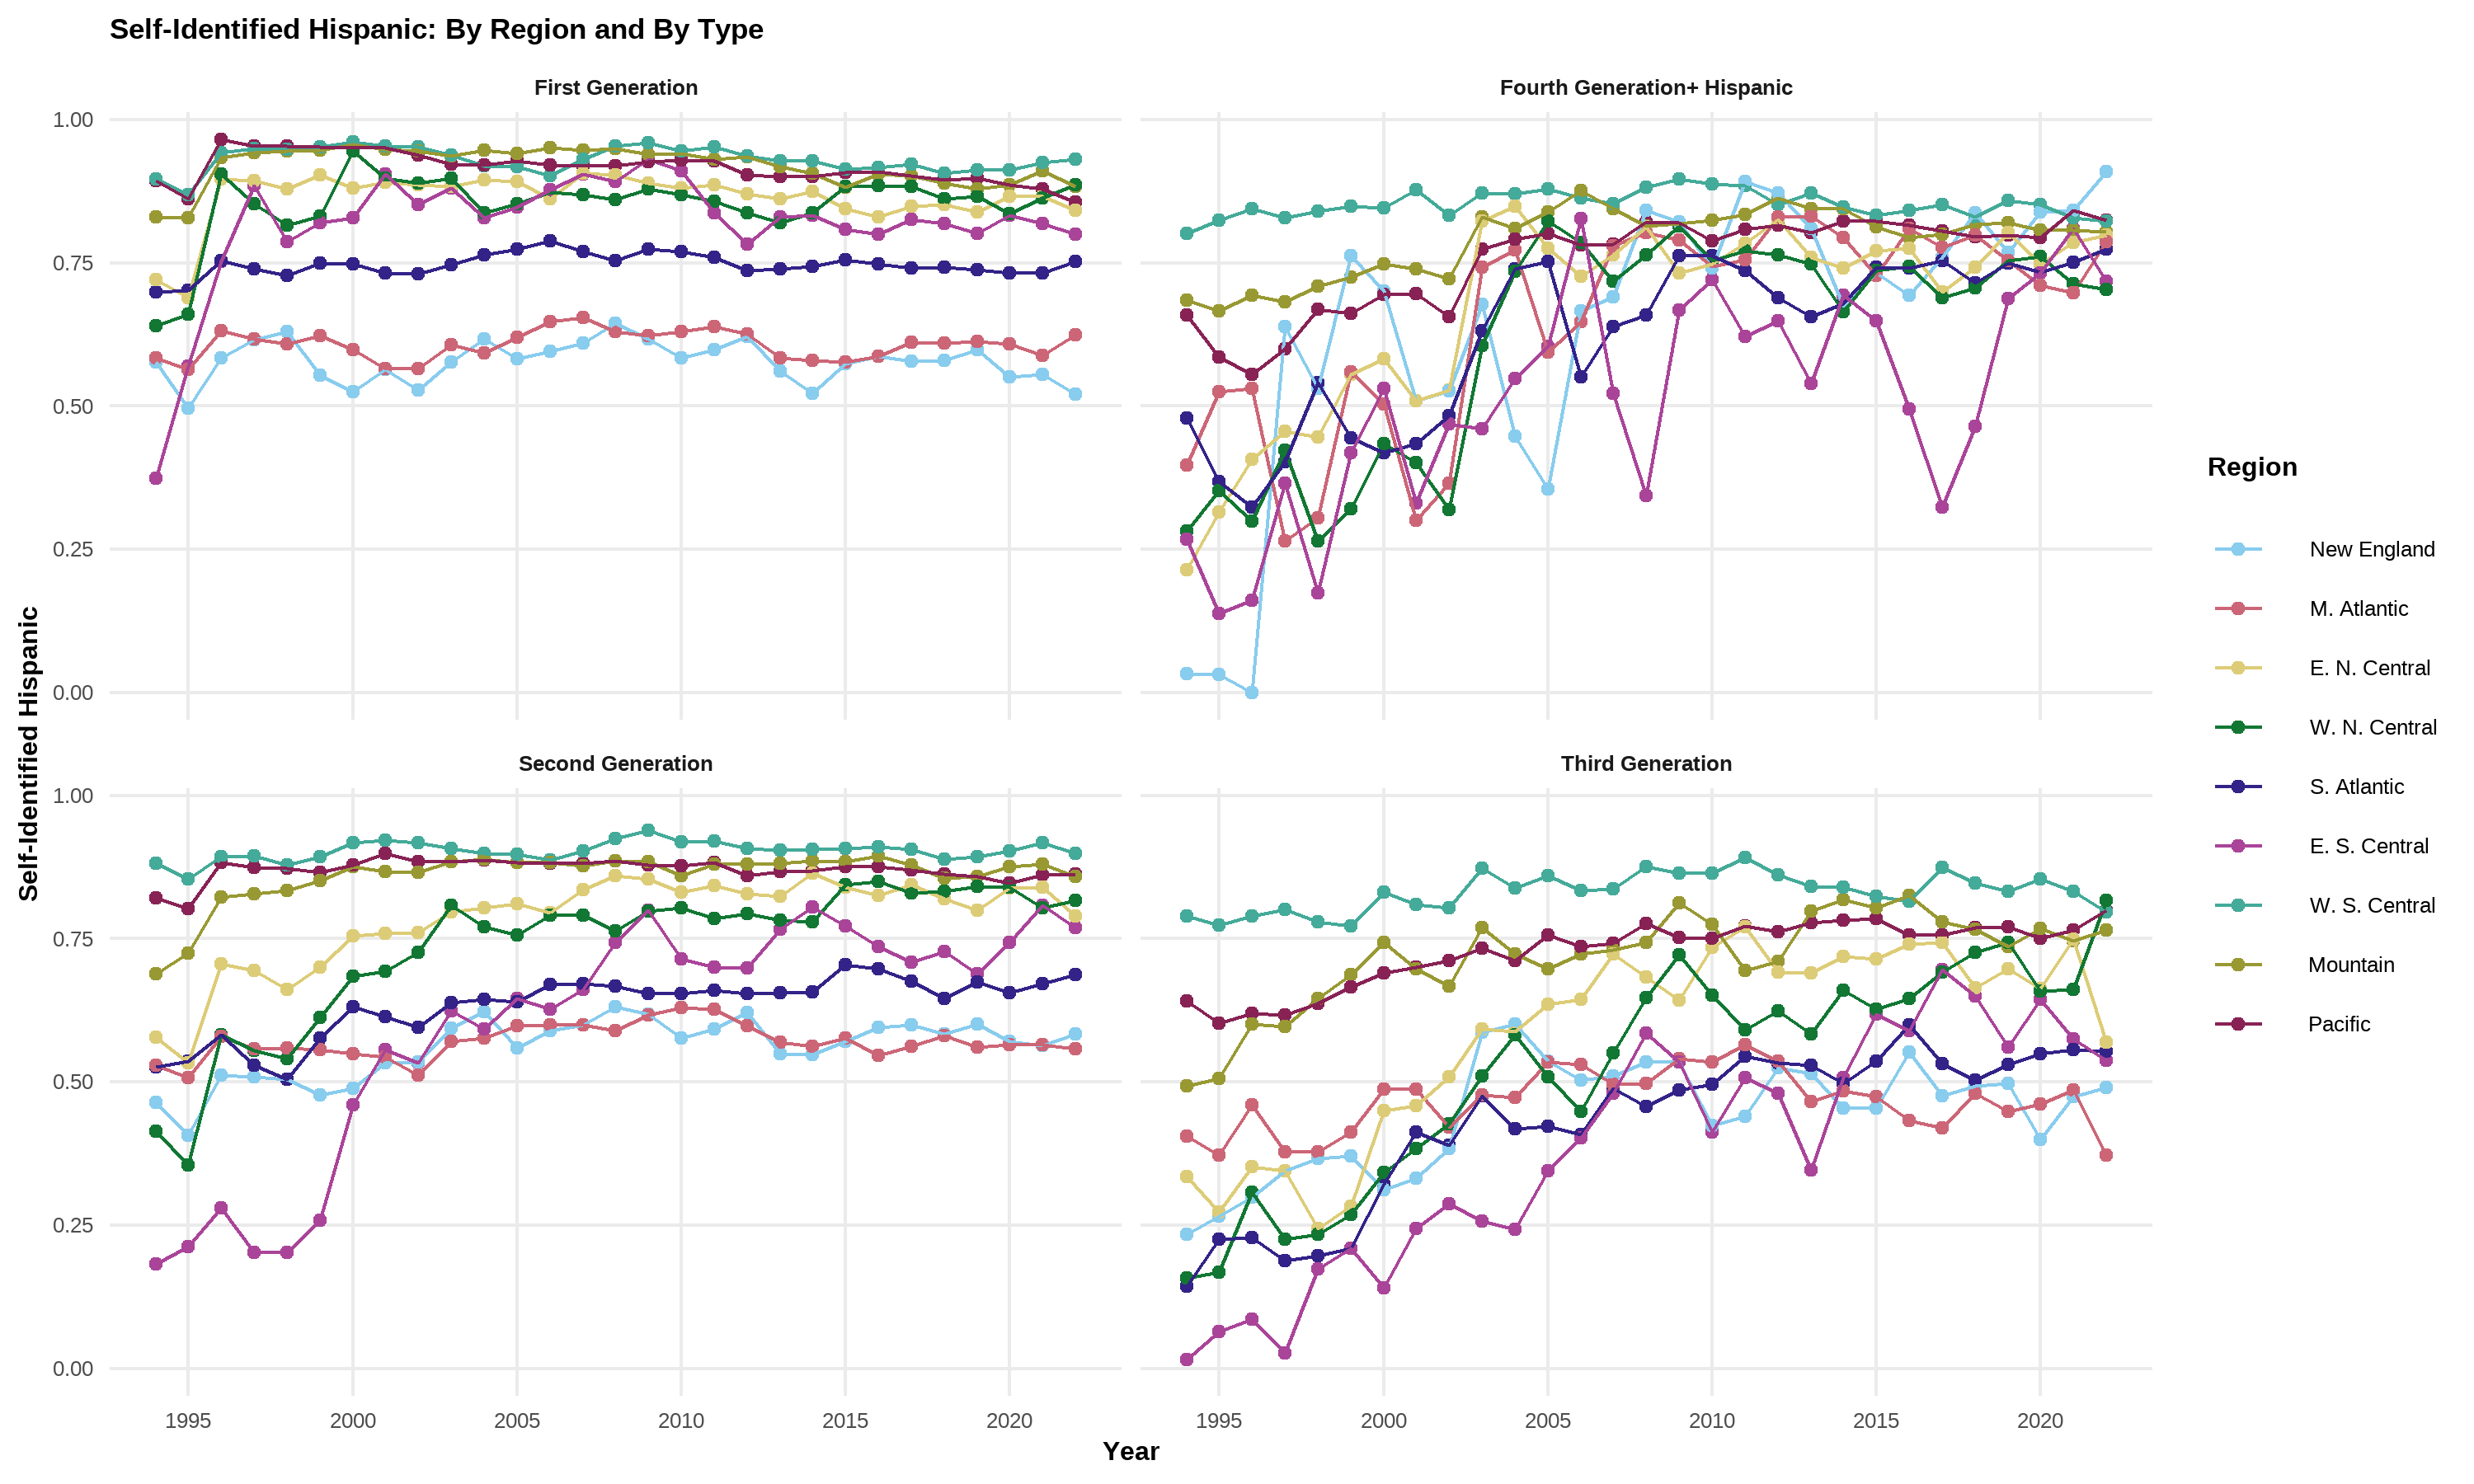
\includegraphics[width=\textwidth]{figure/Hispanics_type.png} 
\label{fig:hispregtype}
\end{figure}
\end{center}

\begin{center}
\begin{figure}[H]
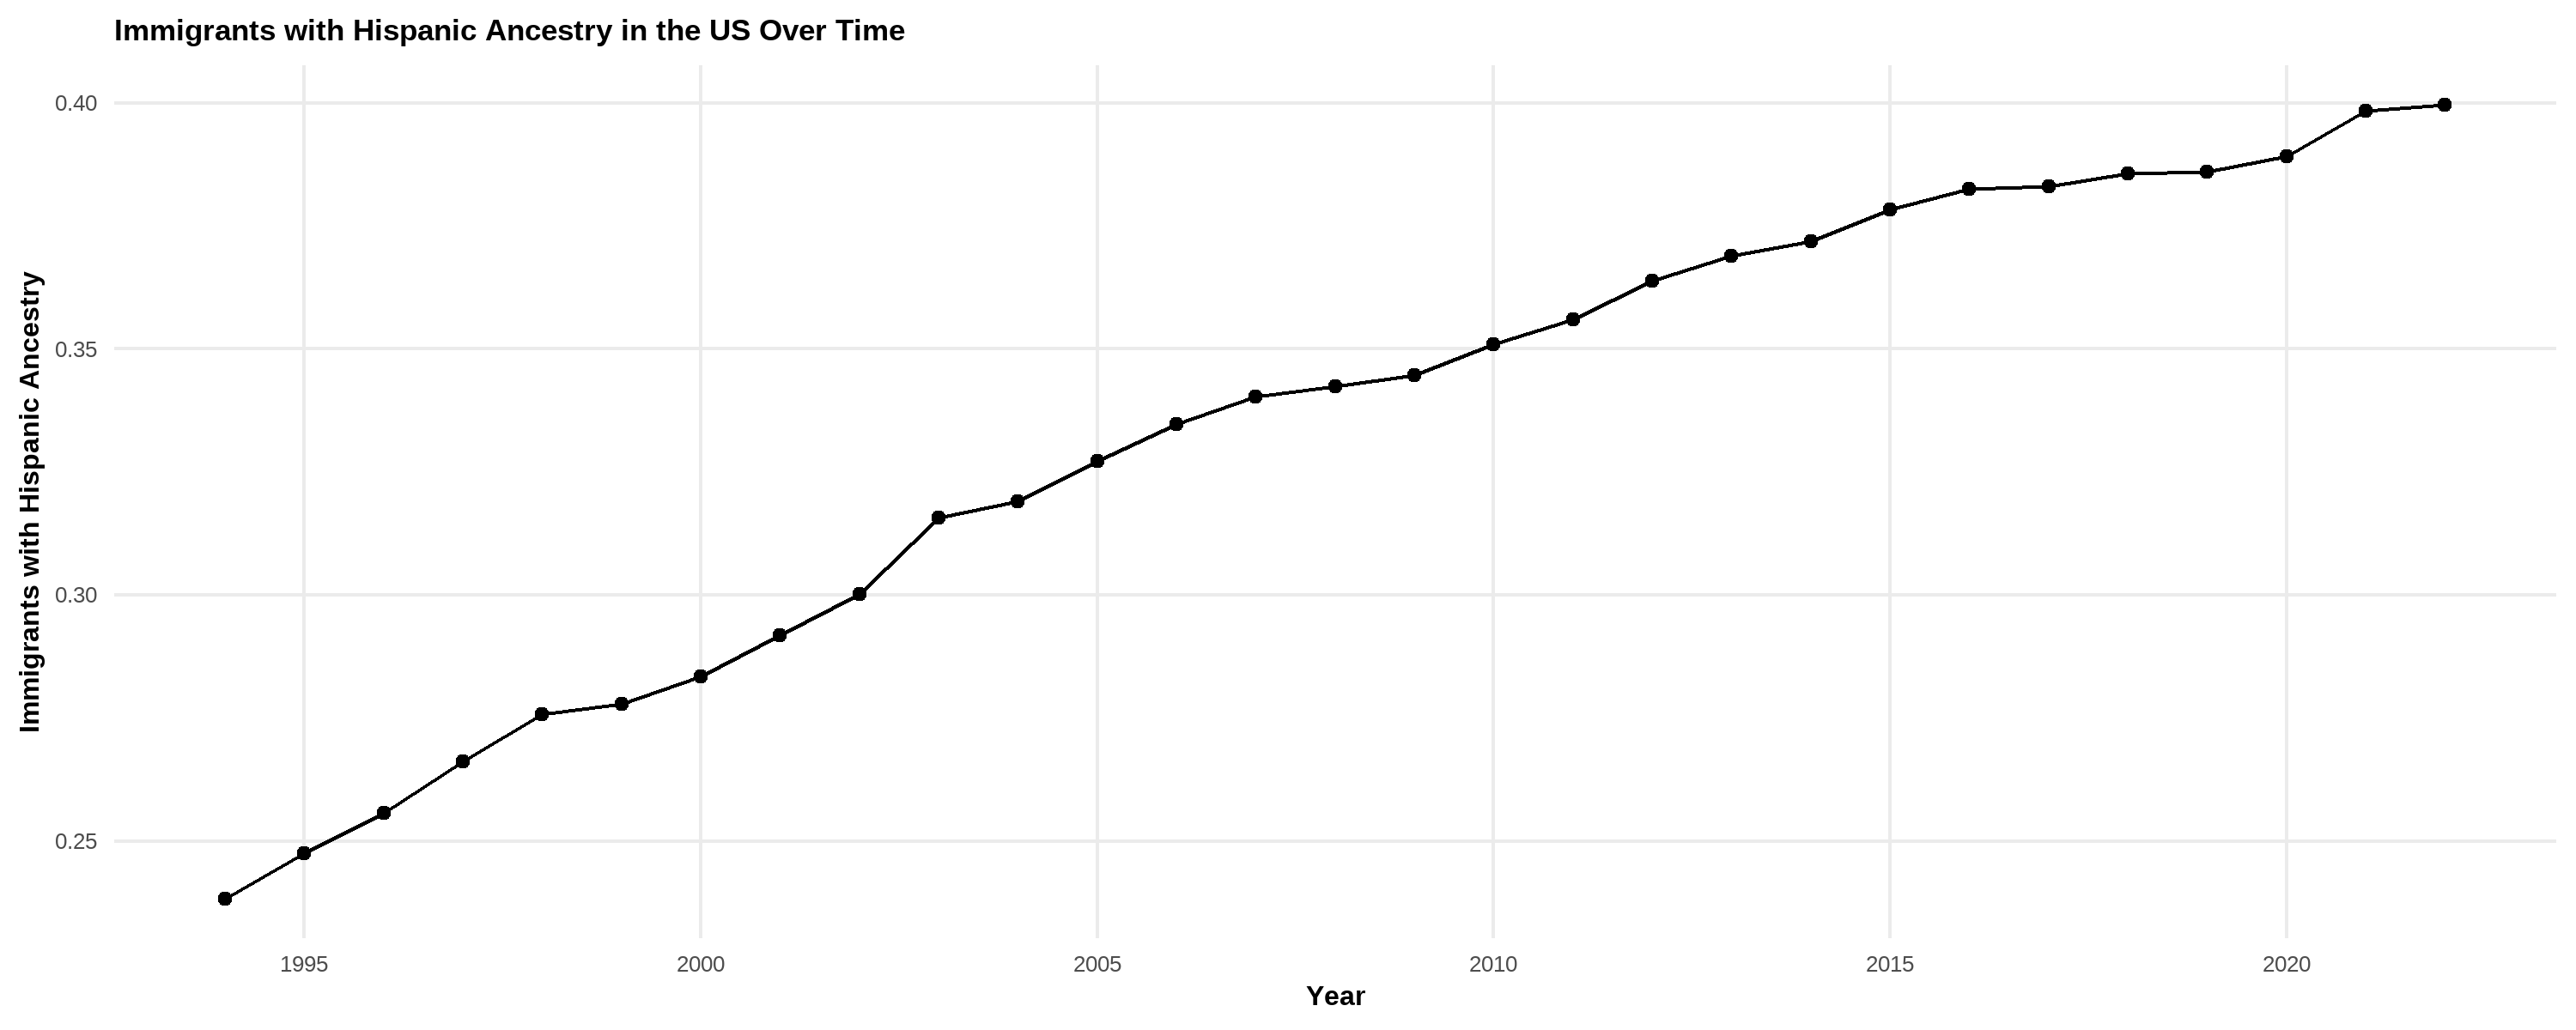
\includegraphics[width=\textwidth]{figure/Hispanics_all_Obj.png} 
\end{figure}
\end{center}


\begin{center}
\begin{figure}[H]
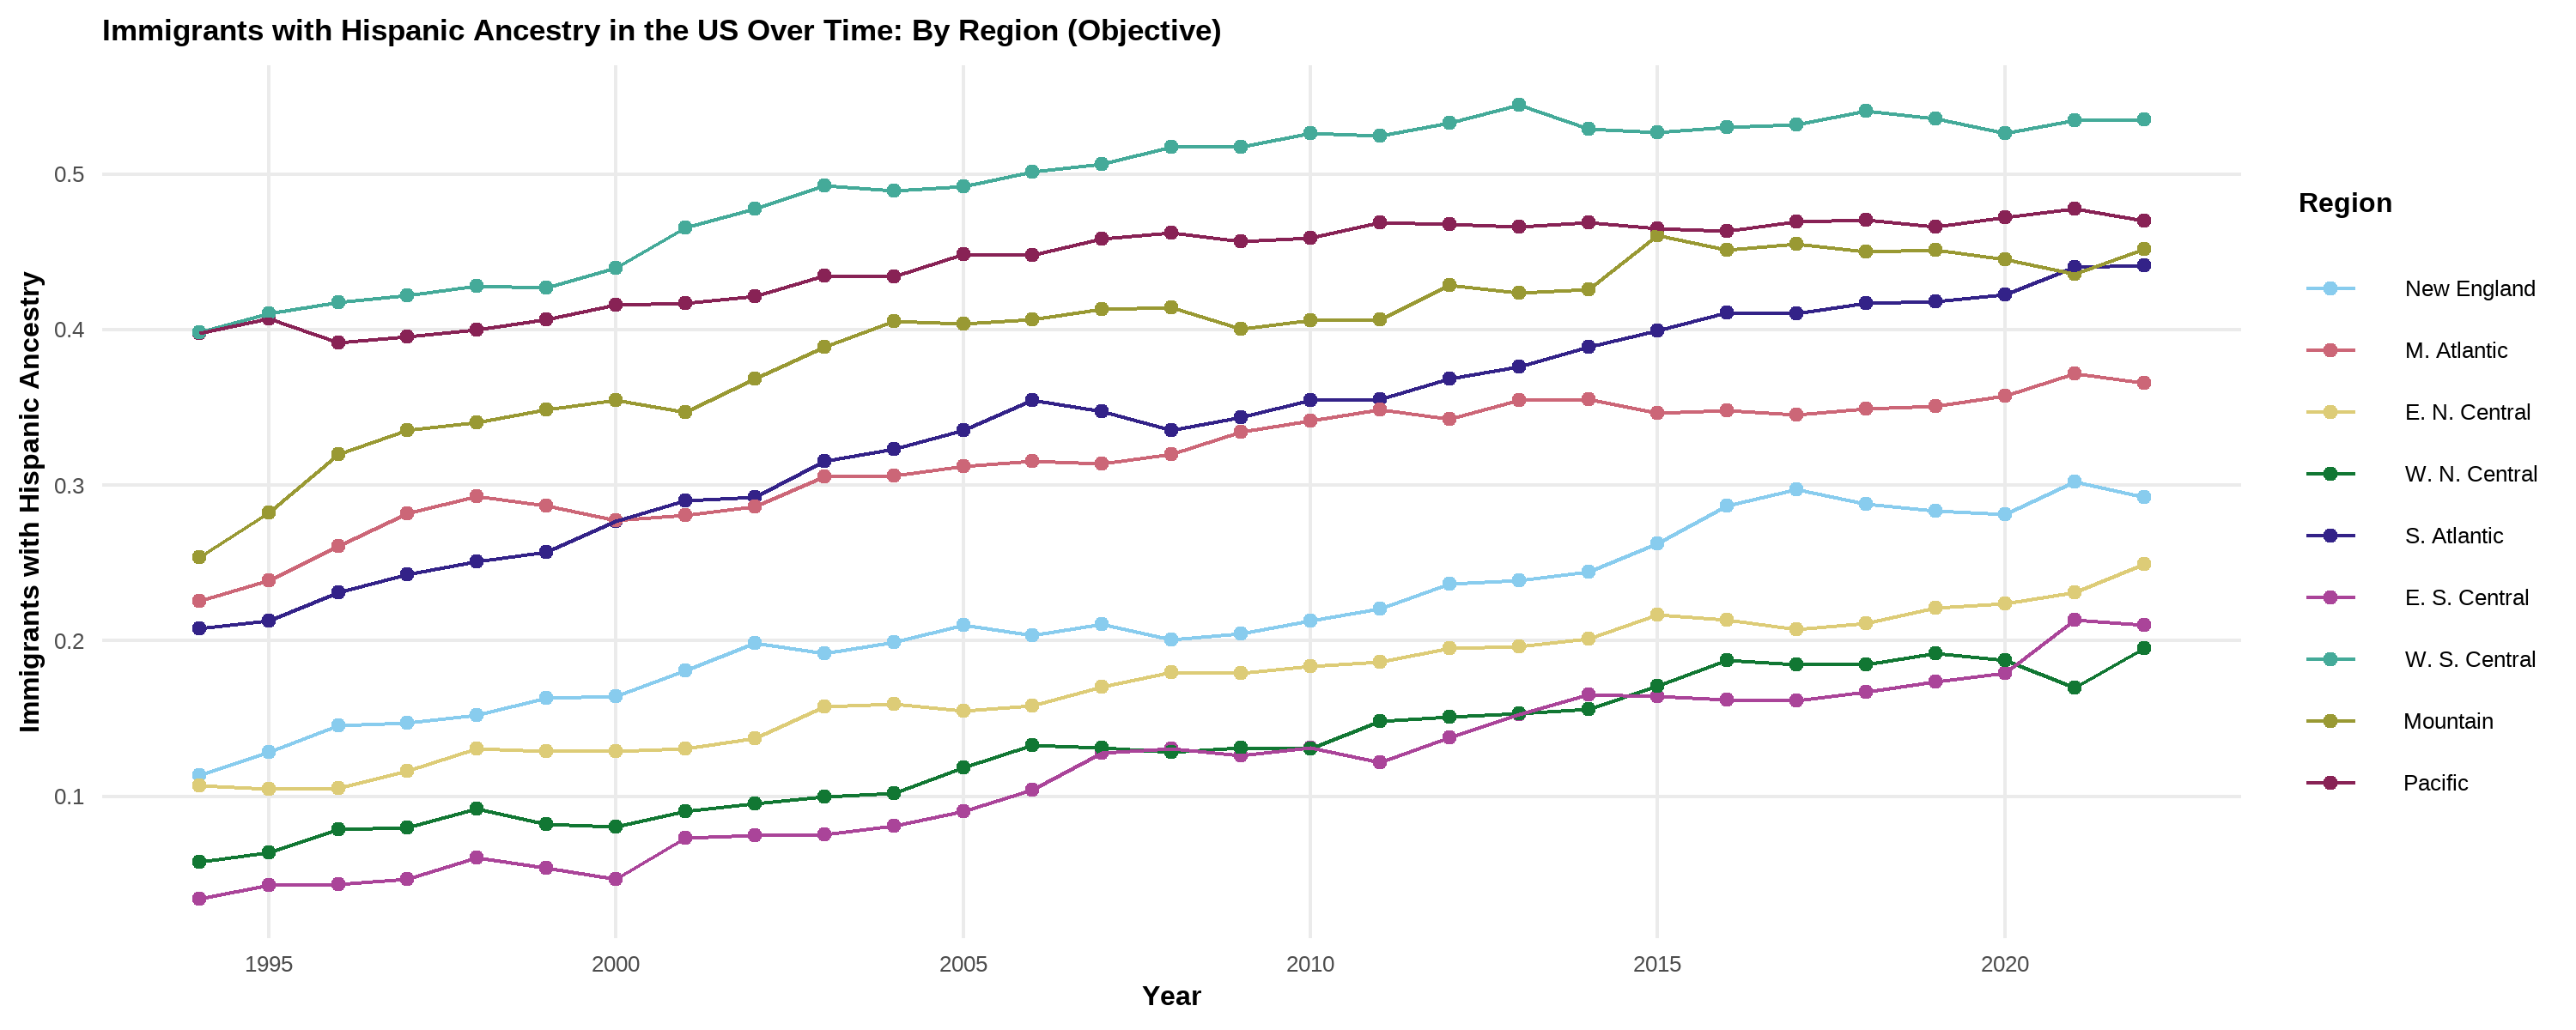
\includegraphics[width=\textwidth]{figure/Hispanics_Obj.png} 
\end{figure}
\end{center}


\newpage
\pagebreak

\begin{center}
\begin{figure}[H]
\caption{Correlation Between Implicit and Explicit Biases: IAT Explicit Bias Question}
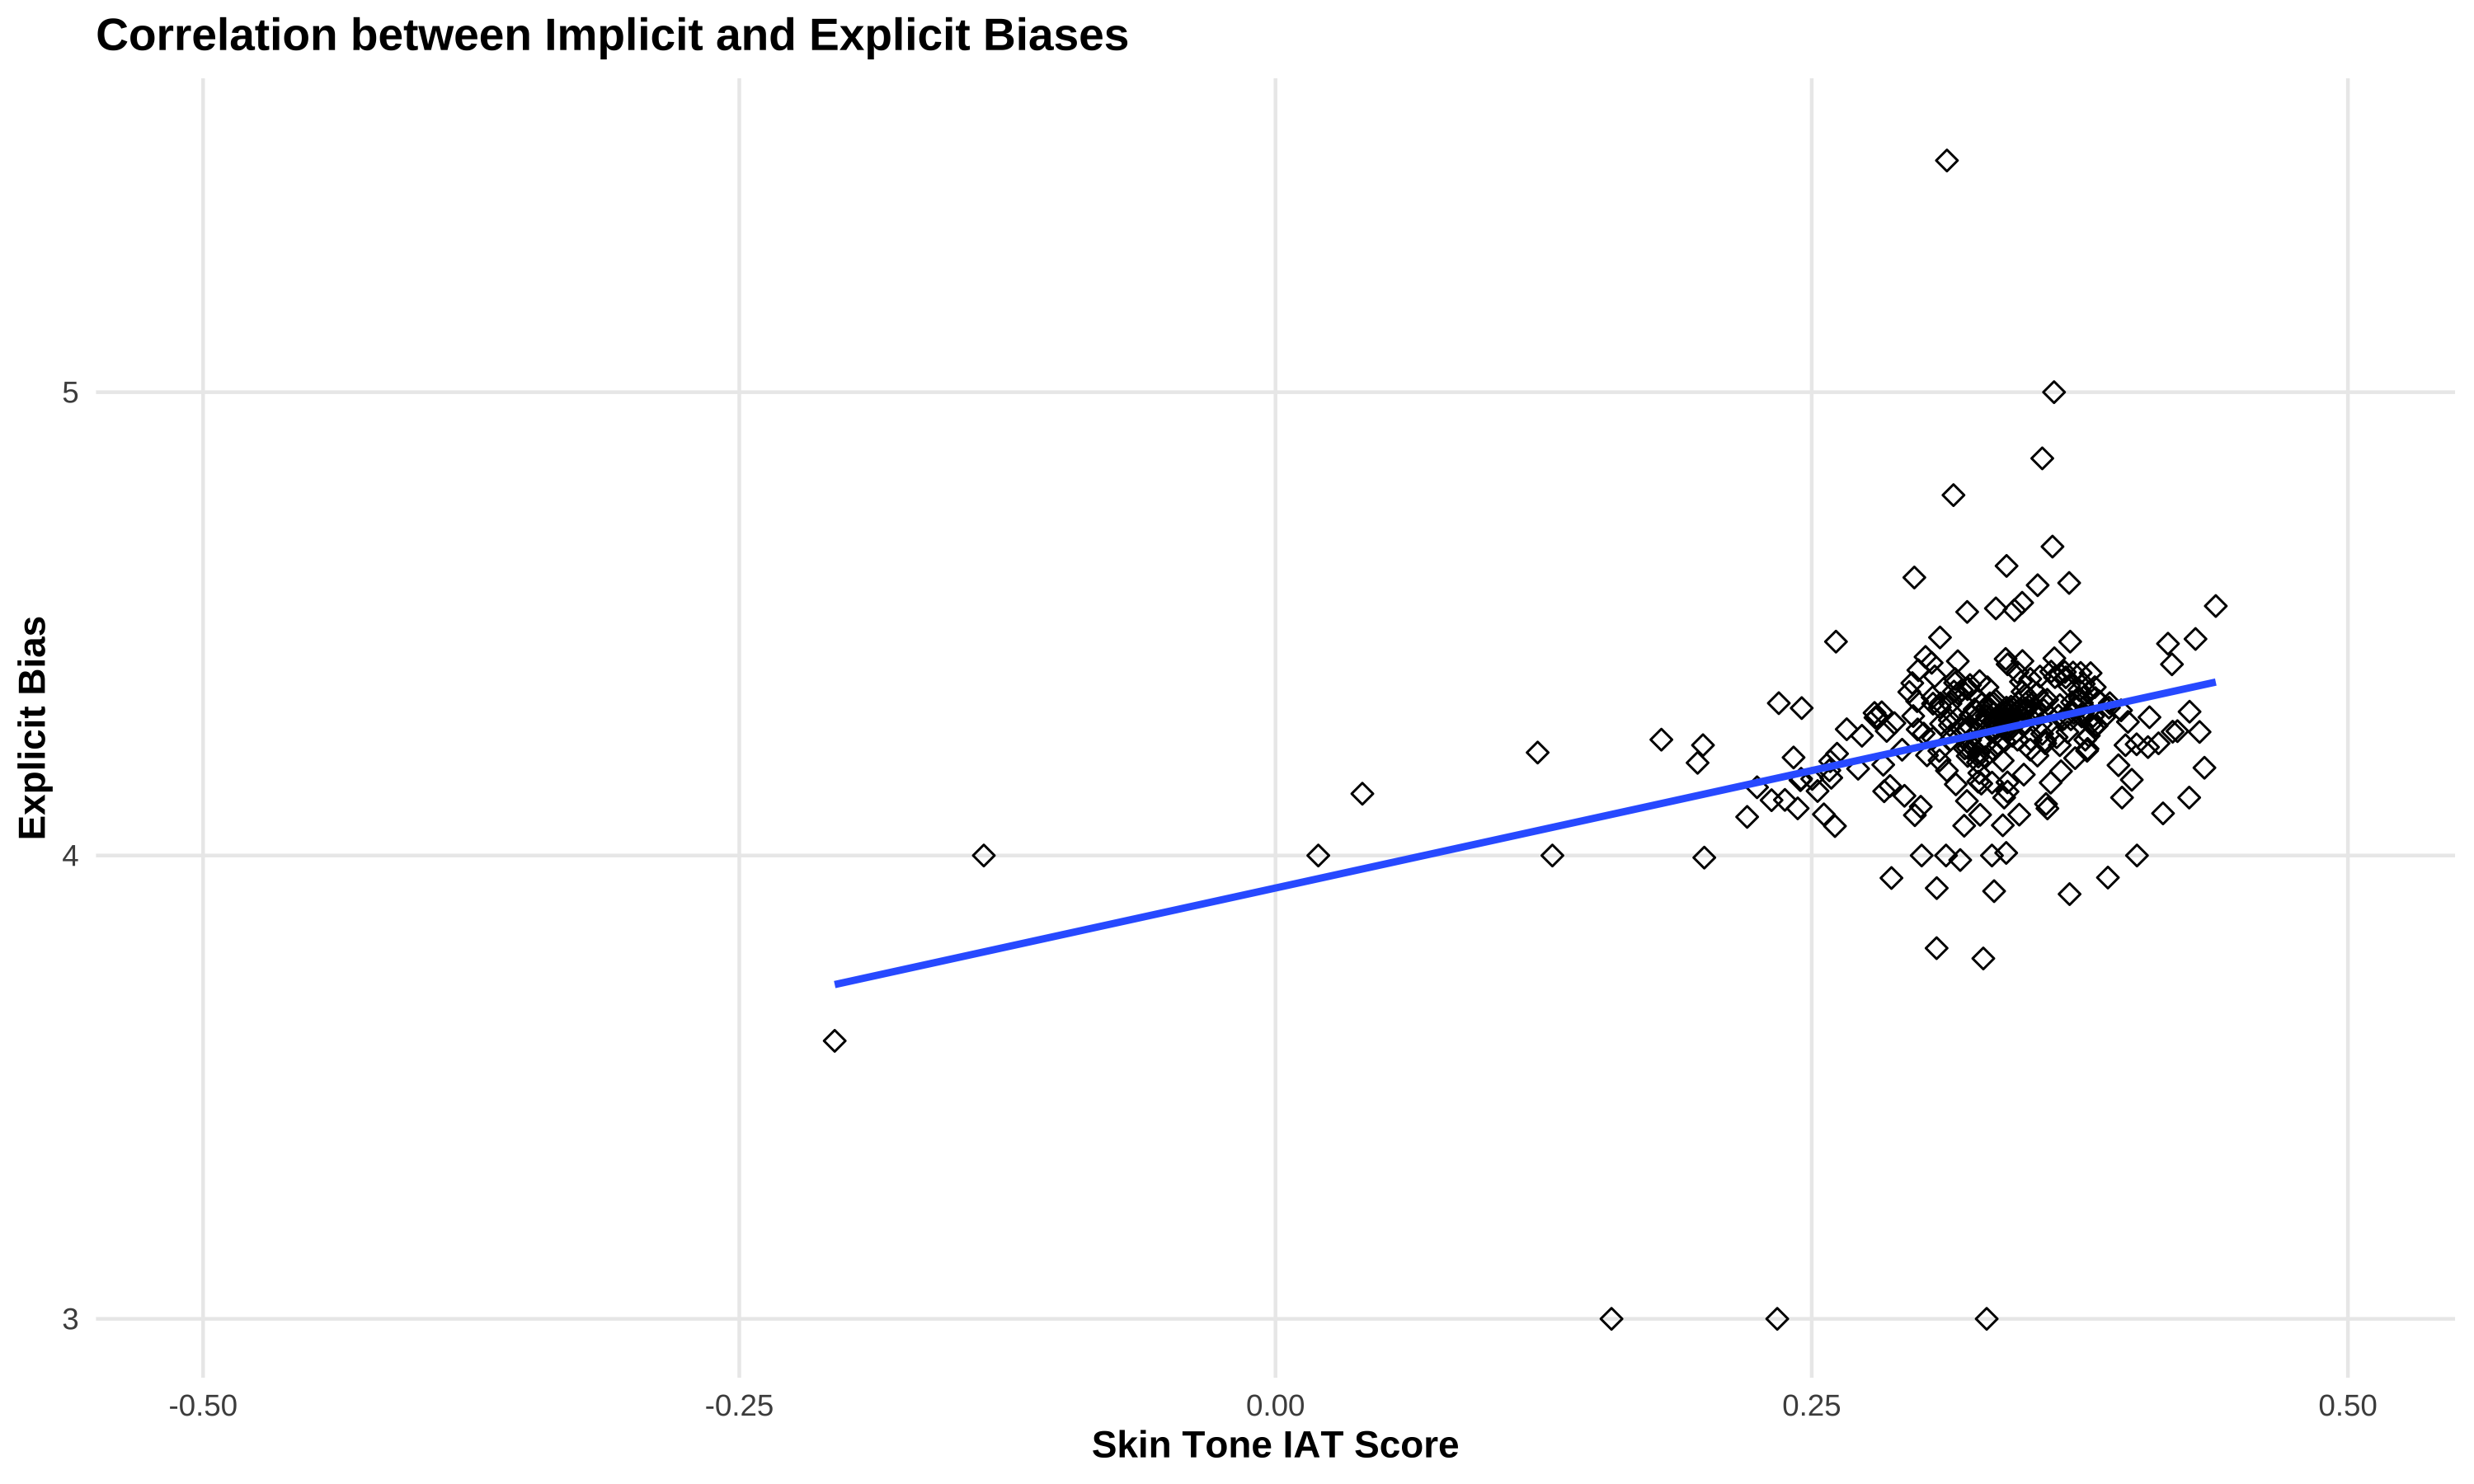
\includegraphics[width=\textwidth]{figure/ImplicitExplicit_scatter.png} 
\label{fig:cor-bias-expl}
\end{figure}
\end{center}

\newpage
\pagebreak

\begin{center}
\begin{figure}[H]
\caption{Correlation Between Implicit and Explicit Biases: GSS Close to Black People Question}
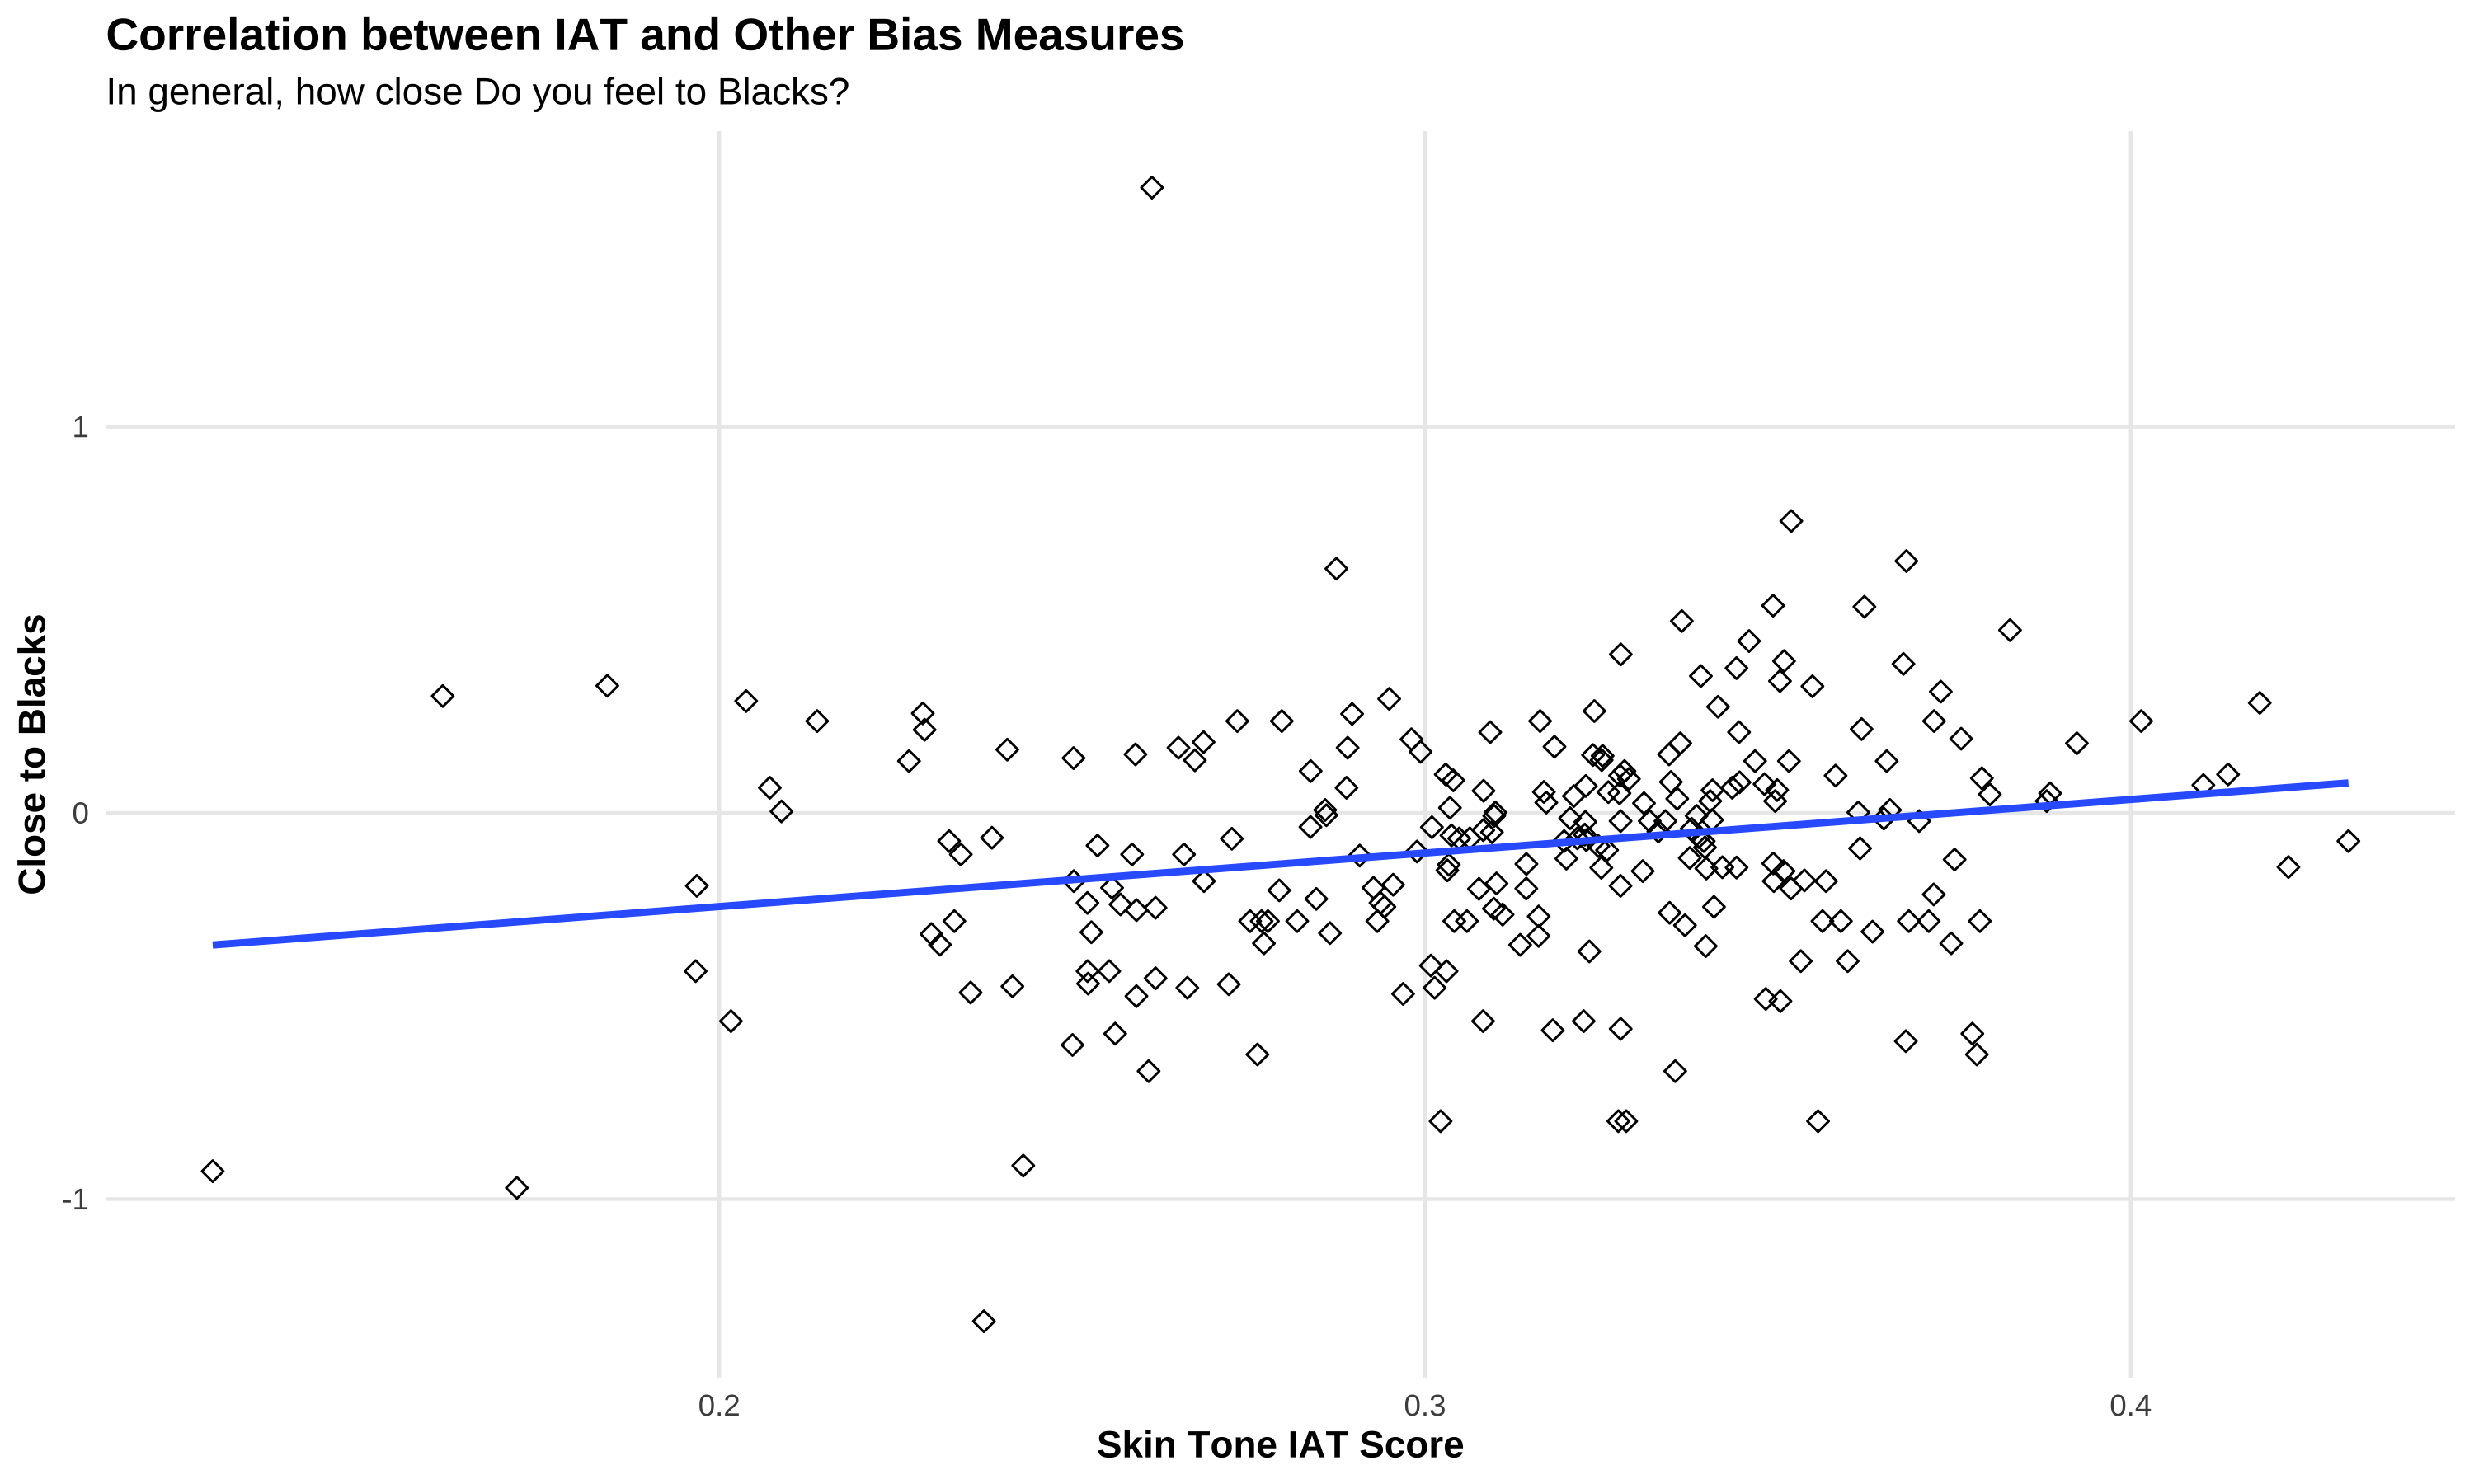
\includegraphics[width=\textwidth]{figure/ImplicitCloseBlk_scatter} 
\label{fig:cor-bias-gss}
\end{figure}
\end{center}

\newpage
\pagebreak

\begin{center}
\begin{figure}[H]
\caption{Correlation Between Implicit and Explicit Biases: GSS Vote for A Black President Question}
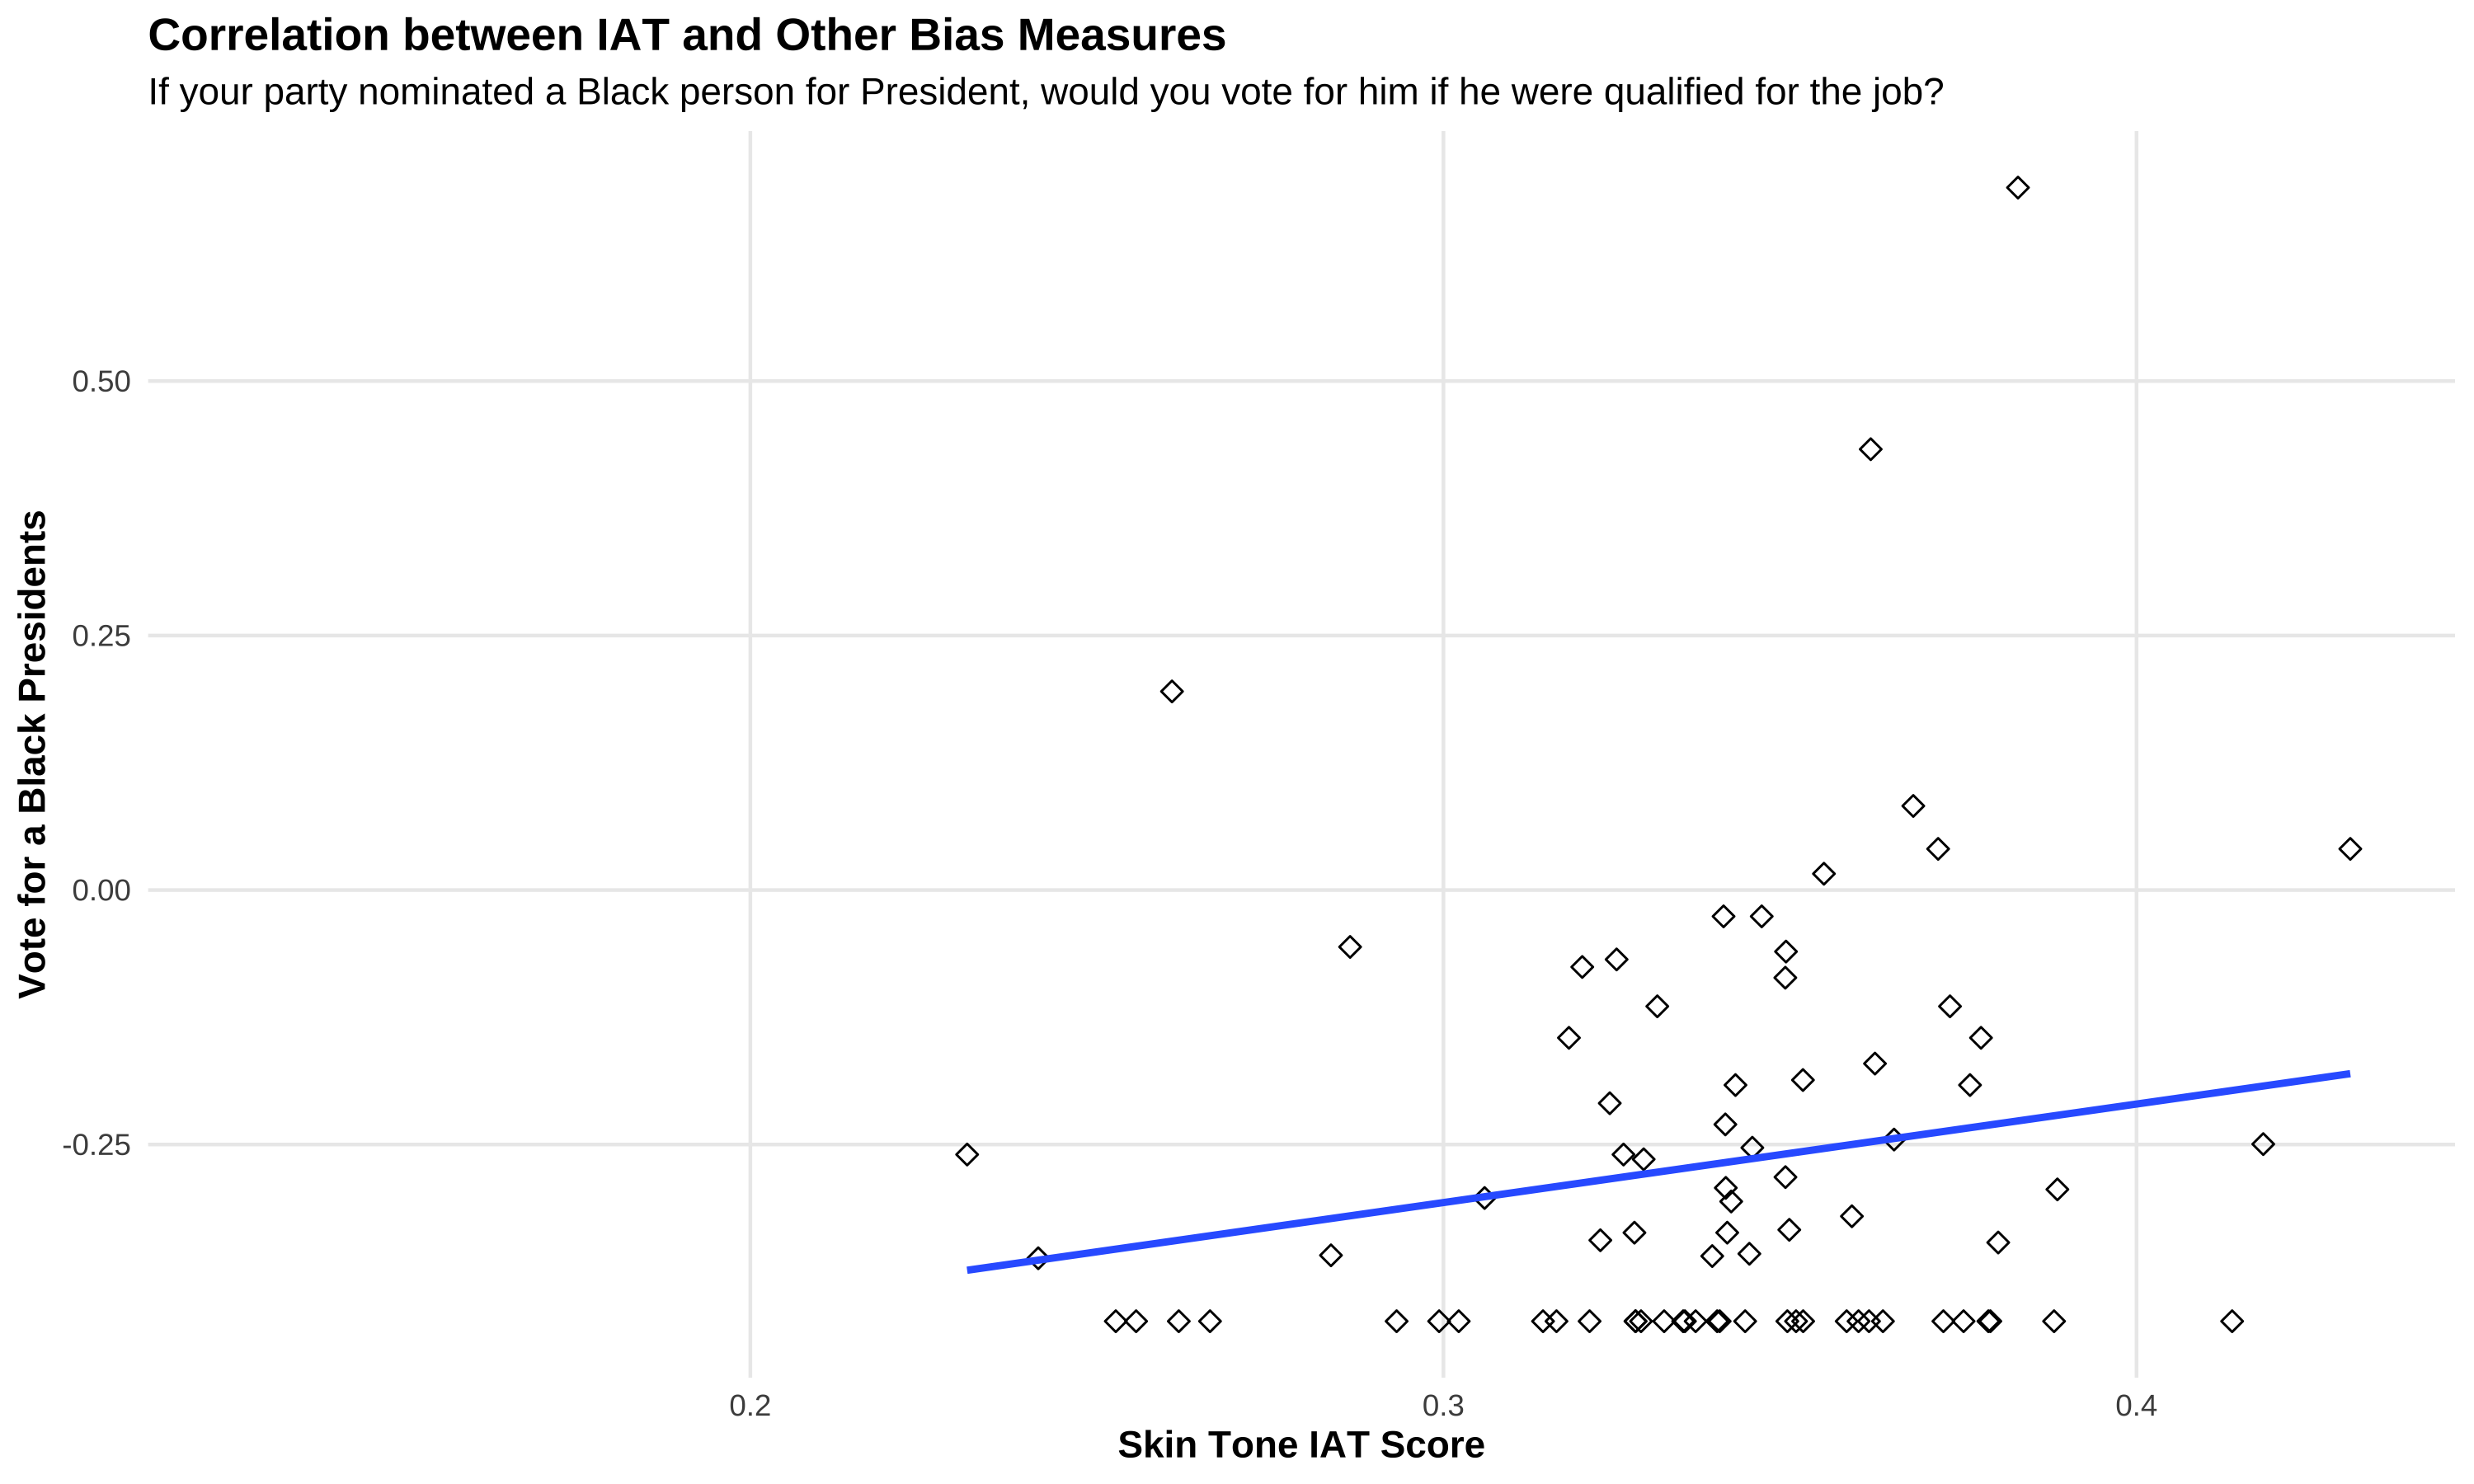
\includegraphics[width=\textwidth]{figure/ImplicitVoteBlk_scatter.png} 
\label{fig:cor-bias-gss-blkpres}
\end{figure}
\end{center}

\newpage
\pagebreak


\begin{figure}[H]
\centering
\caption{Scatter Plot of Non-Hispanic Second-Generation Hispanic-Hispanic Parents on Bias}
\label{scatter-plot-2}
\begin{subfigure}{.9\textwidth}
\caption{Year < 2015}
\centering
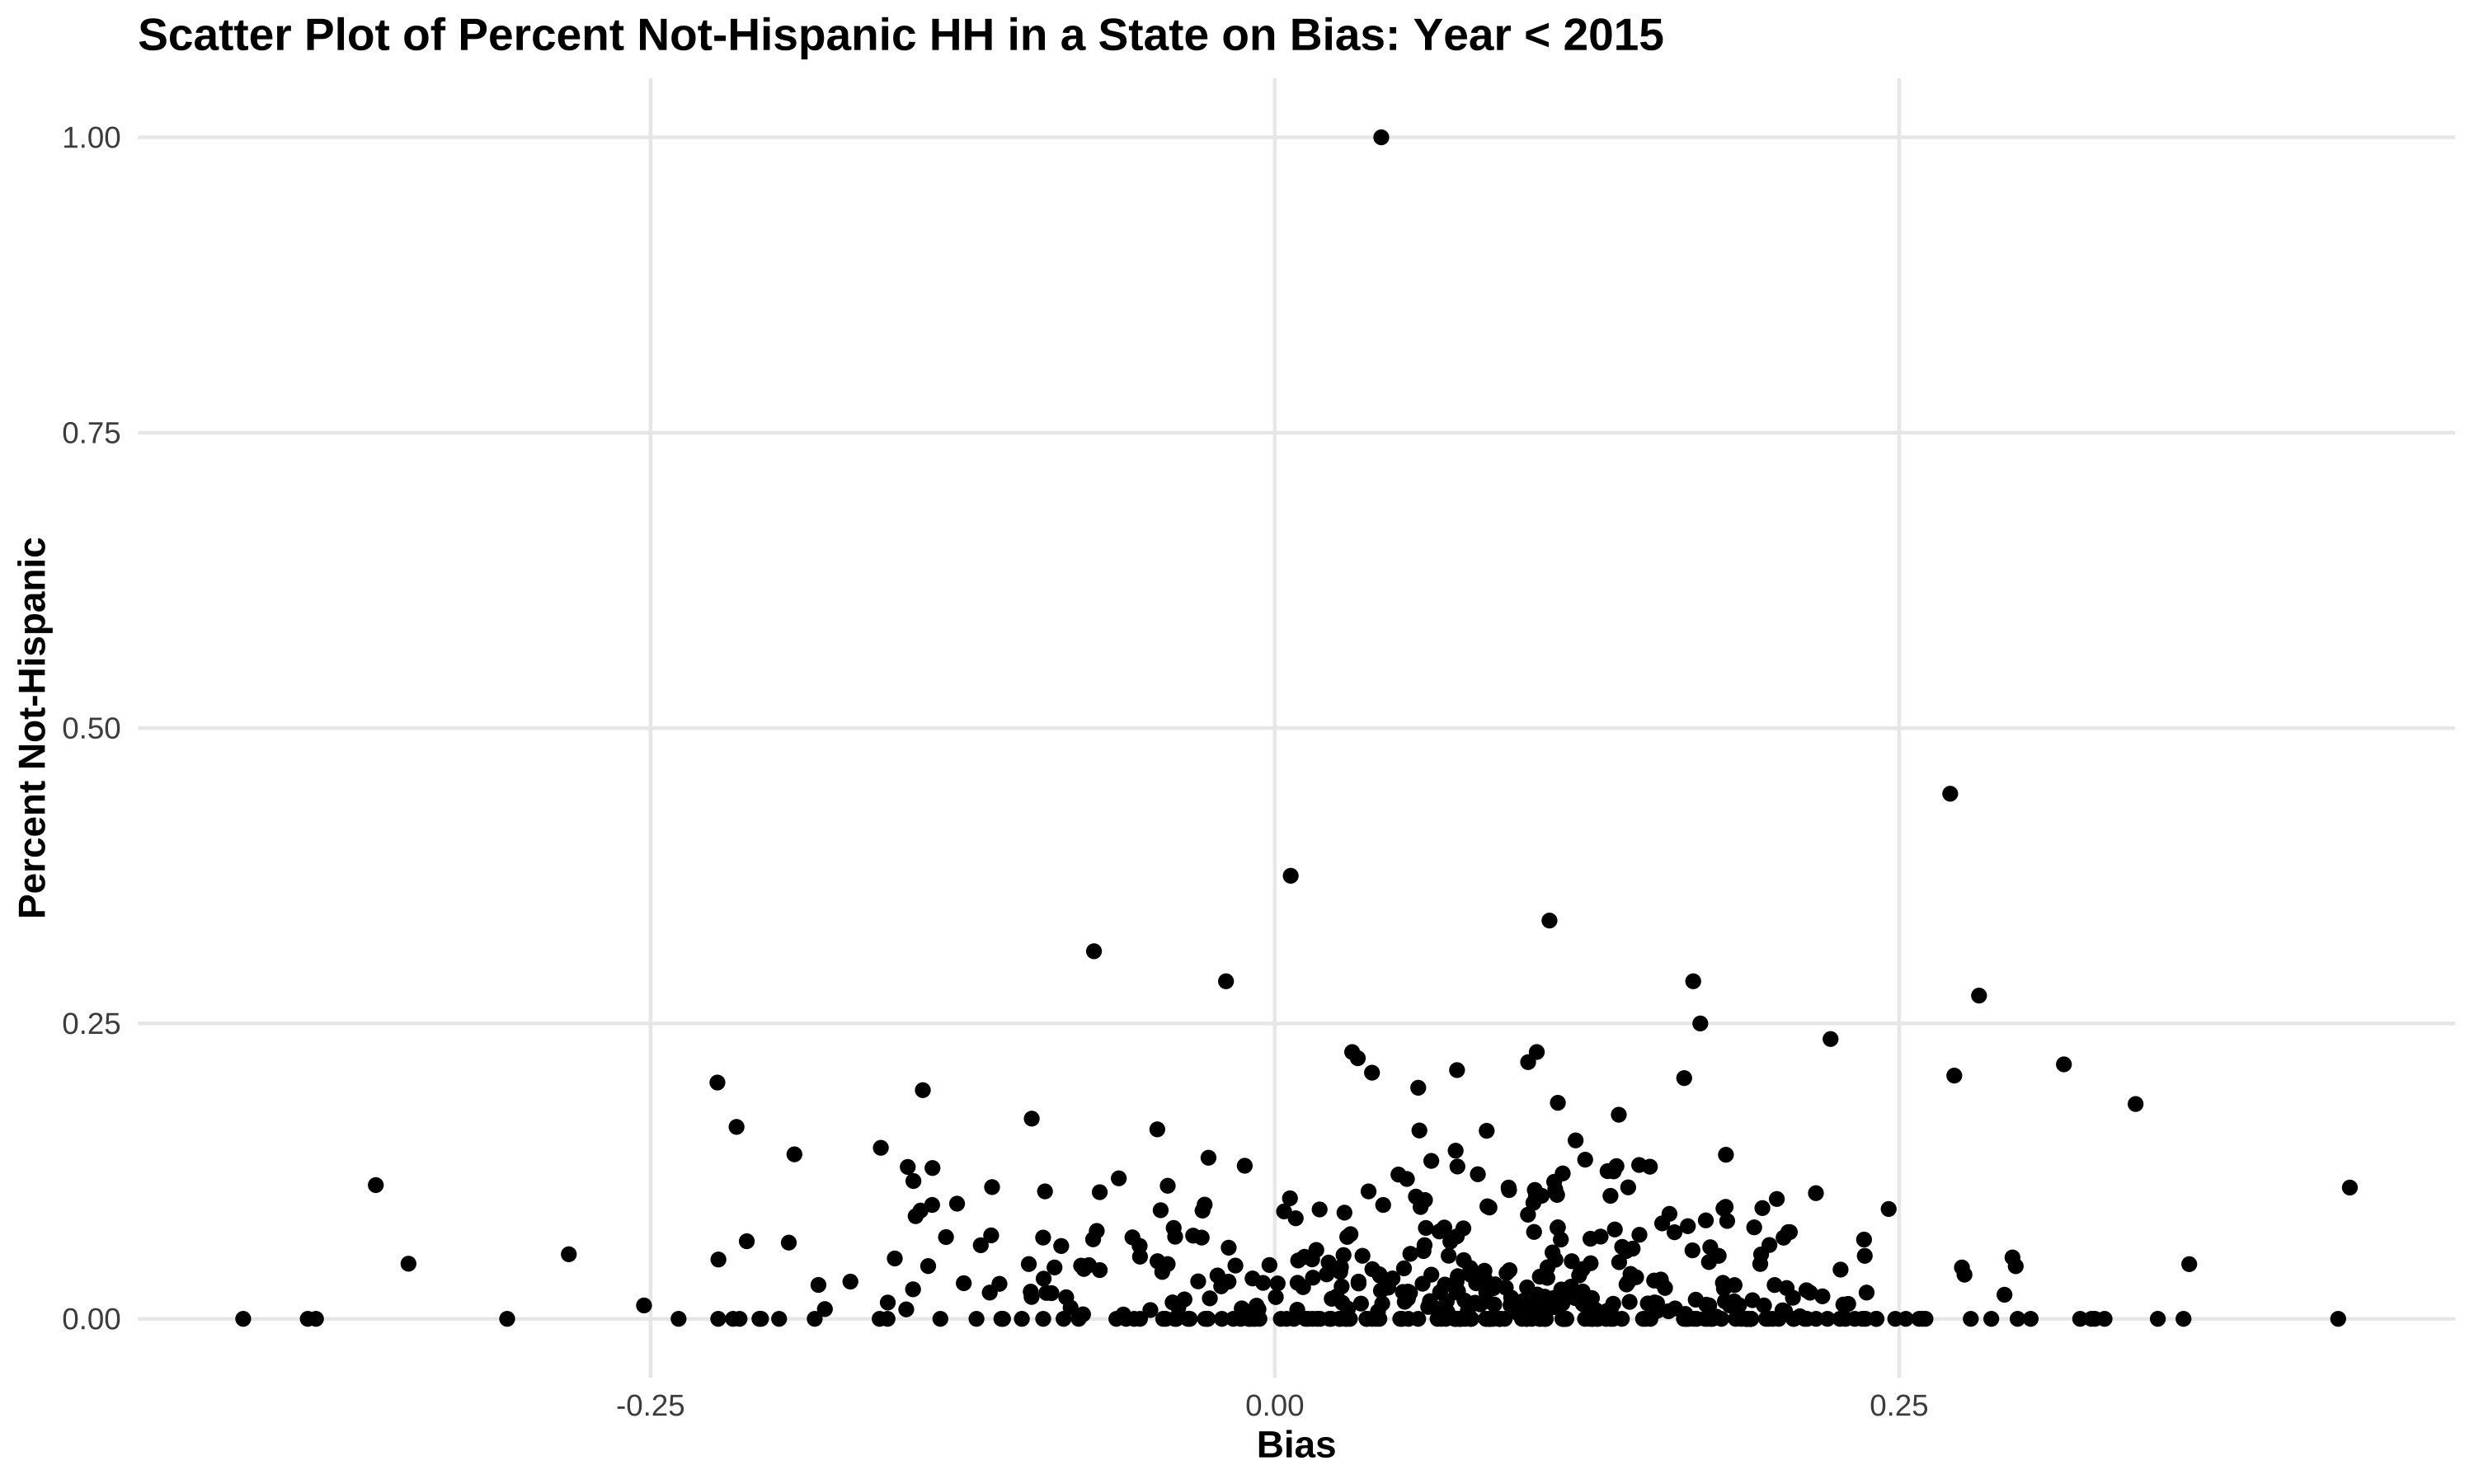
\includegraphics[width=.9\linewidth]{figure/scatter-plot-bias-hh-nothispanic-less2015.png}
\end{subfigure}
\centering
%Second graph
\begin{subfigure}{.9\textwidth}
\caption{Year $\geq$ 2015}
\centering
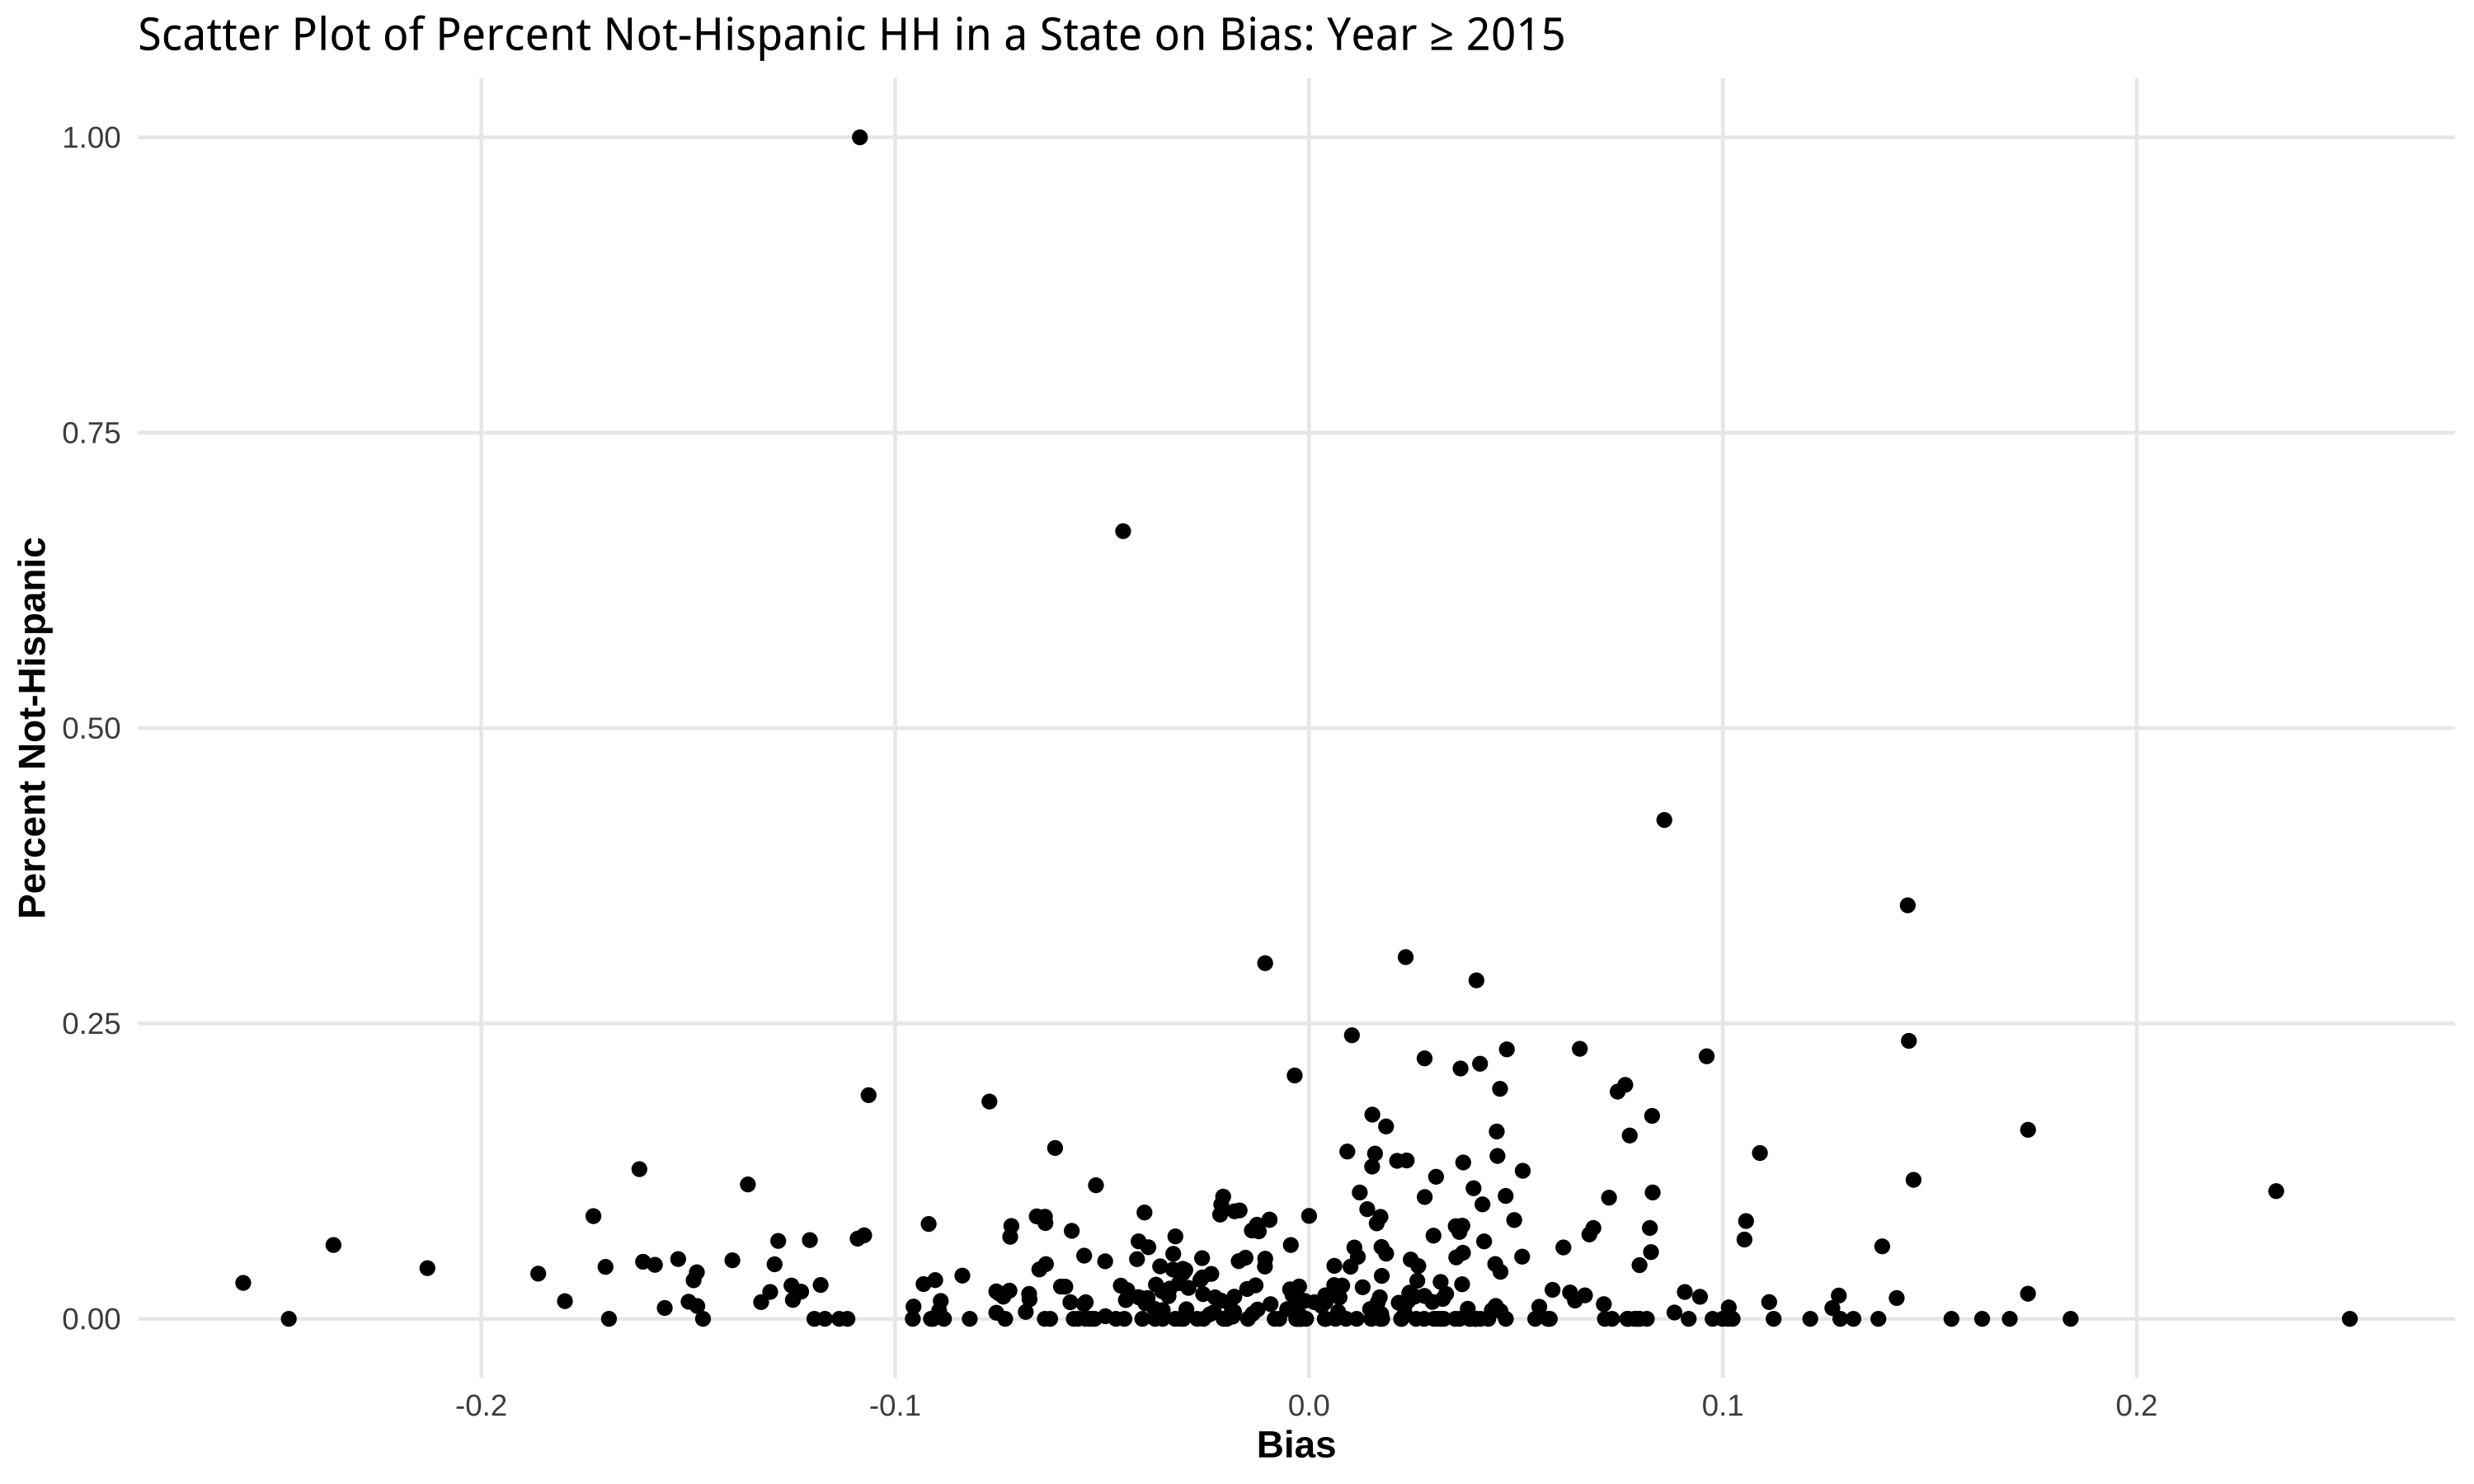
\includegraphics[width=.9\linewidth]{figure/scatter-plot-bias-hh-nothispanic-great2015.png}
\end{subfigure}
\end{figure}

\newpage
\pagebreak


% \begin{center}
% \begin{figure}[H]
% \caption{Scatter Plot of Hispanic second-generation Hispanic-Hispanic Parents on Bias with Year-Region FE}
% 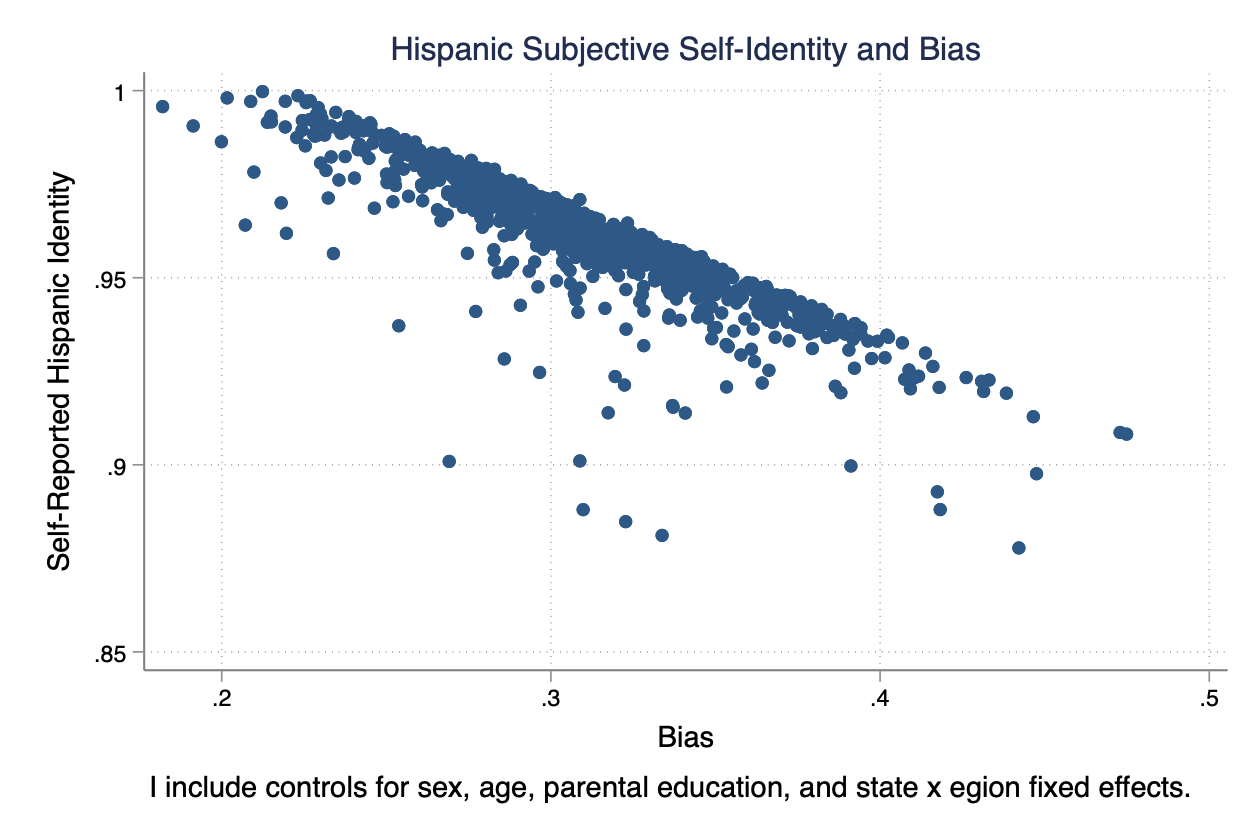
\includegraphics[width=\textwidth]{figure/fe-scatter-plot-byyearstate.png} 
% \label{scatter-plot-3}
% \end{figure}
% \end{center}


\section{Data} % (fold)
\label{sec:data-ap}


\begin{figure}[H]
\centering
\caption{Examples of an Implicit Association Test}
\label{fig:iatexamples}
\begin{subfigure}{.48\textwidth}
\centering
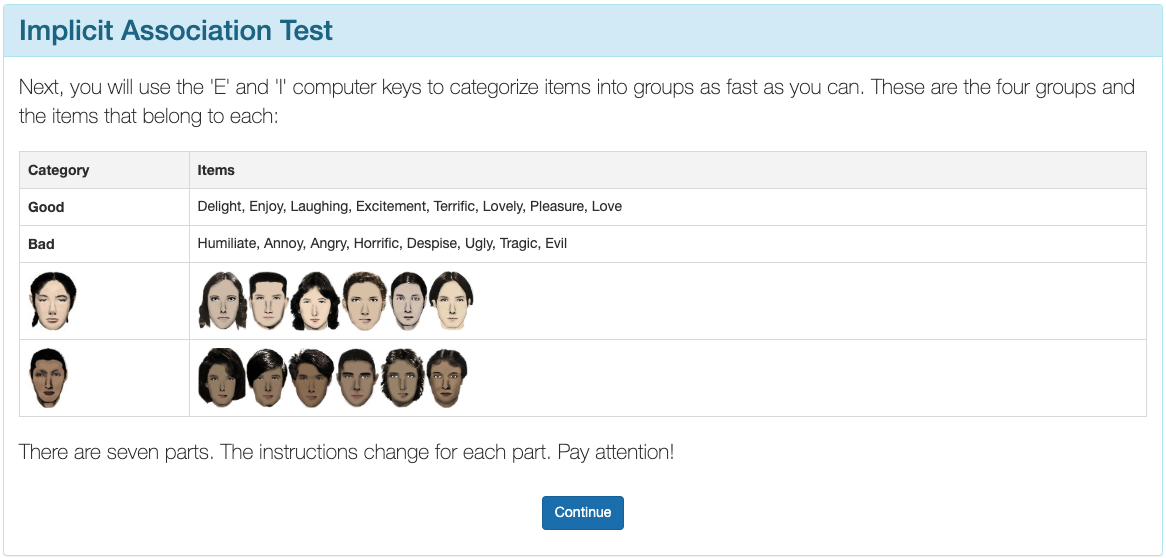
\includegraphics[width=.9\linewidth]{figure/iatexample1.png}
\end{subfigure}
\centering
%Second graph
\begin{subfigure}{.48\textwidth}
\centering
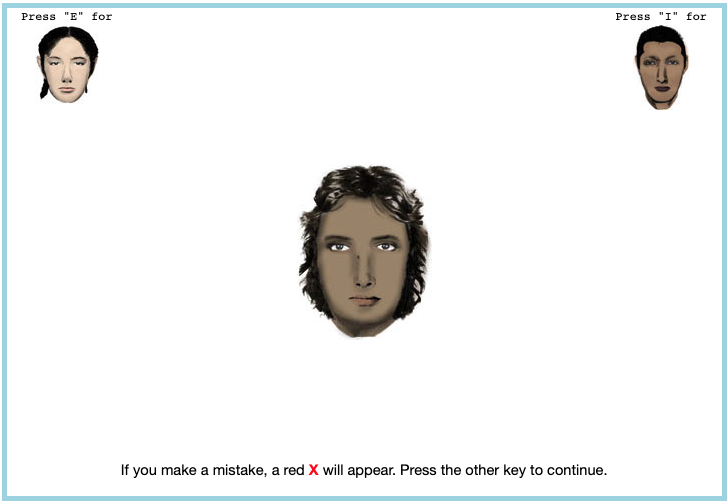
\includegraphics[width=.9\linewidth]{figure/iatexample2.png}
\end{subfigure}
%Third
\begin{subfigure}{.48\textwidth}
\centering
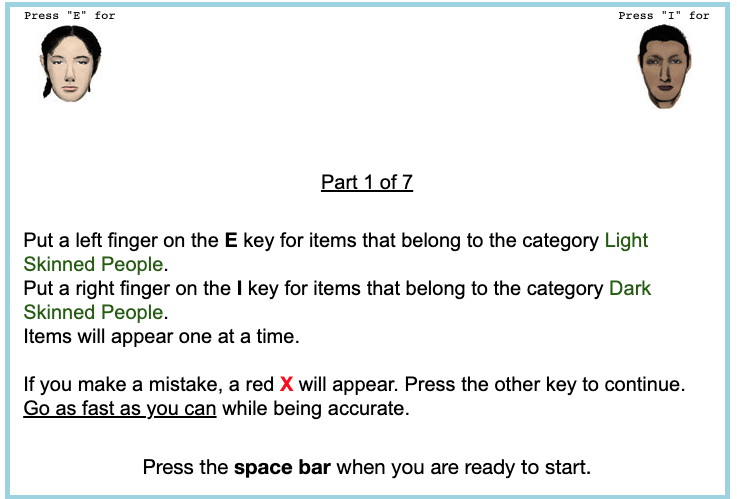
\includegraphics[width=.9\linewidth]{figure/iatexample3.png}
\end{subfigure}
% Fourth
\begin{subfigure}{.48\textwidth}
\centering
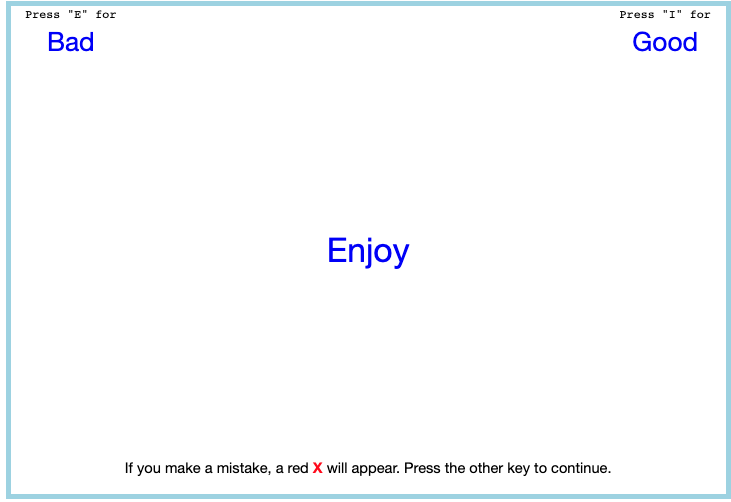
\includegraphics[width=.9\linewidth]{figure/iatexample4.png}
\end{subfigure}
%Fifth
\begin{subfigure}{.48\textwidth}
\centering
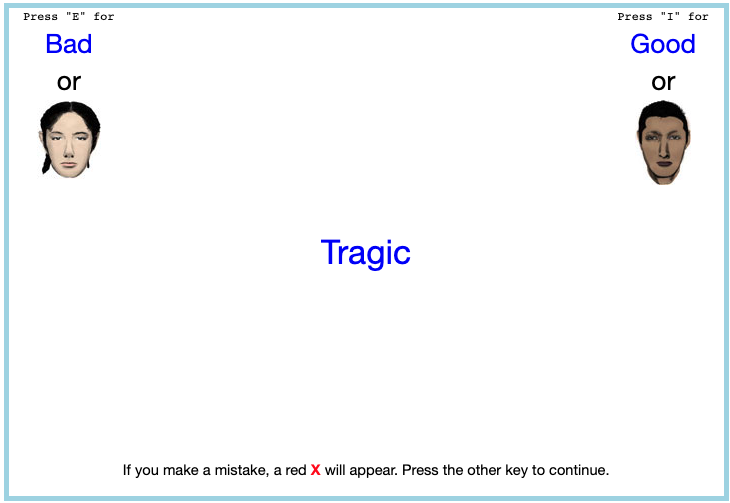
\includegraphics[width=.9\linewidth]{figure/iatexample5.png}
\end{subfigure}
\flushleft\footnotesize{\note{Here are a few examples of what a respondent would see on an implicit association test.}}
\end{figure}


\section{Tables}

\begin{table}[H]

\caption{Number of Children from the Different Types of Parents \label{tab:mat1}}
\centering
\resizebox{\linewidth}{!}{
\begin{threeparttable}
\begin{tabular}[t]{>{}lcccc}
\toprule
\multicolumn{1}{c}{ } & \multicolumn{4}{c}{Perent's Type} \\
\cmidrule(l{3pt}r{3pt}){2-5}
Parents' Type & \specialcell{White Father \\ White Mother} & \specialcell{White Father \\ Hispanic Mother} & \specialcell{Hispanic Father \\ White Mother} & \specialcell{Hispanic Father \\ Hispanic Mother}\\
\midrule
\textbf{Observations} & \specialcell{3,828,024\\(0.95)} & \specialcell{24,306\\(0.01)} & \specialcell{35,841\\(0.01)} & \specialcell{135,300\\(0.03)}\\
\bottomrule
\end{tabular}
\begin{tablenotes}
\item[1] The data is restricted to people interviewed between 1994 and 2019, also White, married, and between the ages of 18 and 65. I identify the ethnicity of a person's parents through the parent's place of birth. A parent is Hispanic if both her parents were born in a Spanish-speaking country. A parent is White if born parents were born in the United States.
\end{tablenotes}
\end{threeparttable}}
\end{table}


\newpage

\begin{table}[H]

\caption{Couples' Type \label{tab:mat2}}
\centering
\resizebox{\linewidth}{!}{
\begin{threeparttable}
\begin{tabular}[t]{>{}lcccc}
\toprule
\multicolumn{1}{c}{ } & \multicolumn{4}{c}{Couples' Type} \\
\cmidrule(l{3pt}r{3pt}){2-5}
  & \specialcell{White Husband \\ White Wife} & \specialcell{White Husband \\ Hispanic Wife} & \specialcell{Hispanic Husband \\ White Wife} & \specialcell{Hispanic Husband \\ Hispanic Wife}\\
\midrule
\textbf{Observations} & \specialcell{1,286,731\\(0.97)} & \specialcell{7,178\\(0.01)} & \specialcell{7,606\\(0.01)} & \specialcell{20,911\\(0.02)}\\
\bottomrule
\end{tabular}
\begin{tablenotes}
\item[1] The data is restricted to people interviewed in 1970 and 1960 and also White and married. I identify the ethnicity of a person through their place of birth. A parent is Hispanic if they were born in a Spanish-speaking country. A parent is White if they were born in the United States.
\item[2] The table includes information on the proportion of the four types of synthetic parents that I have constructed.
\end{tablenotes}
\end{threeparttable}}
\end{table}


\newpage

\begin{table}[H]

\caption{Children's outcome using parent's place of birth \label{tab:c&p1}}
\centering
\resizebox{0.9\linewidth}{!}{ % <-- Add this line to scale down the table
\begin{threeparttable}
\begin{tabular}[t]{lcccccc}
\toprule
\multicolumn{1}{c}{ } & \multicolumn{4}{c}{Father's and Mother's Ethnicities} & \multicolumn{2}{c}{Differences} \\
\cmidrule(l{3pt}r{3pt}){2-5} \cmidrule(l{3pt}r{3pt}){6-7}
Variables & \specialcell{White Father \\ White Mother \\ (WW) \\ (i)} & \specialcell{White Father \\ Hispanic Mother \\ (WH) \\ (ii)} & \specialcell{Hispanic Father \\ White Mother \\ (HW) \\ (iii)} & \specialcell{Hispanic Father \\ Hispanic Mother \\ (HH) \\ (iv)} & \specialcell{HH - WW \\ (v)} & \specialcell{HW - WH \\ (vi)}\\
\midrule
\textbf{Panel A: Parent’s} & \textbf{} & \textbf{} & \textbf{} & \textbf{} & \textbf{} & \textbf{}\\
\hspace{1em}Husband’seducation (Total Years) & \specialcell{13.05\\(2.44)} & \specialcell{12.32\\(3.33)} & \specialcell{10.65\\(4.39)} & \specialcell{8.93\\(4.41)} & \specialcell{-4.11\\(0.02)} & \specialcell{-1.67\\(0.04)}\\
\hspace{1em}Wife’seducation (Total Years) & \specialcell{12.74\\(2.12)} & \specialcell{11.03\\(3.92)} & \specialcell{11.54\\(3.12)} & \specialcell{8.6\\(4.13)} & \specialcell{-4.13\\(0.02)} & \specialcell{0.51\\(0.04)}\\
\hspace{1em}Total Household seducation (Total Years) & \specialcell{25.78\\(4.08)} & \specialcell{23.35\\(6.51)} & \specialcell{22.19\\(6.69)} & \specialcell{17.54\\(7.83)} & \specialcell{-4.13\\(0.02)} & \specialcell{0.51\\(0.04)}\\
\textbf{Panel B: Education} & \textbf{} & \textbf{} & \textbf{} & \textbf{} & \textbf{} & \textbf{}\\
\addlinespace
\hspace{1em}Men’s education (Total Years) & \specialcell{13.91\\(2.39)} & \specialcell{13.58\\(2.35)} & \specialcell{13.21\\(2.32)} & \specialcell{12.91\\(2.26)} & \specialcell{-1.00\\(0.01)} & \specialcell{-0.36\\(0.03)}\\
\hspace{1em}Women’s education (Total Years) & \specialcell{14.29\\(2.41)} & \specialcell{13.87\\(2.47)} & \specialcell{13.42\\(2.35)} & \specialcell{13.27\\(2.37)} & \specialcell{-1.01\\(0.01)} & \specialcell{-0.46\\(0.03)}\\
\textbf{Panel C: Employment and Earnings} & \textbf{} & \textbf{} & \textbf{} & \textbf{} & \textbf{} & \textbf{}\\
\hspace{1em}Men’s Employment Rate & \specialcell{0.95\\(0.22)} & \specialcell{0.94\\(0.23)} & \specialcell{0.92\\(0.26)} & \specialcell{0.93\\(0.26)} & \specialcell{-0.02\\(0)} & \specialcell{-0.02\\(0)}\\
\hspace{1em}Women’s Employment Rate & \specialcell{0.96\\(0.2)} & \specialcell{0.95\\(0.22)} & \specialcell{0.93\\(0.25)} & \specialcell{0.94\\(0.24)} & \specialcell{-0.02\\(0)} & \specialcell{-0.02\\(0)}\\
\addlinespace
\hspace{1em}Men’s Log Hourly Earnings & \specialcell{2.48\\(0.45)} & \specialcell{2.41\\(0.45)} & \specialcell{2.4\\(0.44)} & \specialcell{2.41\\(0.43)} & \specialcell{-0.07\\(0.01)} & \specialcell{-0.00\\(0.02)}\\
\hspace{1em}Women’s Hourly Earnings & \specialcell{2.33\\(0.49)} & \specialcell{2.33\\(0.46)} & \specialcell{2.27\\(0.45)} & \specialcell{2.3\\(0.41)} & \specialcell{-0.02\\(0.01)} & \specialcell{-0.06\\(0.02)}\\
\hspace{1em}Men’s Log Annual Earnings & \specialcell{10.25\\(1.01)} & \specialcell{10.08\\(1.05)} & \specialcell{10.04\\(1.06)} & \specialcell{10.01\\(1.04)} & \specialcell{-0.25\\(0.01)} & \specialcell{-0.04\\(0.03)}\\
\hspace{1em}Women’s Hourly Earnings & \specialcell{9.46\\(1.78)} & \specialcell{9.54\\(1.64)} & \specialcell{9.47\\(1.57)} & \specialcell{9.53\\(1.52)} & \specialcell{0.07\\(0.02)} & \specialcell{-0.07\\(0.06)}\\
\textbf{Panel D: Hispanic Identity} & \textbf{} & \textbf{} & \textbf{} & \textbf{} & \textbf{} & \textbf{}\\
\addlinespace
\hspace{1em}Men & \specialcell{0.05} & \specialcell{0.81} & \specialcell{0.88} & \specialcell{0.97} &  & \\
\hspace{1em}Women & \specialcell{0.06} & \specialcell{0.85} & \specialcell{0.87} & \specialcell{0.97} &  & \\
\bottomrule
\end{tabular}
\begin{tablenotes}
\item[1] The data is restricted to native-born United States citizens between 1994 and 2019 who are also White and between the ages of 25 and 40. I identify the ethnicity of a person's parents through the parent's place of birth. A parent is Hispanic if they were born in a Spanish-speaking country. A parent is White if they were born in the United States.
\item[2] In each column, I present the average statistics of the different types of people based on the ethnicities of their parents. In column one, I show the summary statistics of children of White fathers and White mothers. In column two, I present the summary statistics of children of White fathers and Hispanic mothers. In column three, I show the summary statistics of children of Hispanic fathers and White mothers. In column four, I present the summary statistics of children of Hispanic fathers and mothers.
\item[3] Columns five and six have data on the HH--WW gaps (column five) and the HW--WH gaps (column six).
\end{tablenotes}
\end{threeparttable}}
\end{table}


\newpage

\begin{table}[H]

\caption{Children's outcome using parent's place of birth Only for those that Identify as Hispanic \label{tab:c&p2}}
\centering
\resizebox{0.9\linewidth}{!}{ % <-- Add this line to scale down the table
\begin{threeparttable}
\begin{tabular}[t]{lcccccc}
\toprule
\multicolumn{1}{c}{ } & \multicolumn{4}{c}{Father's and Mother's Ethnicities} & \multicolumn{2}{c}{Differences} \\
\cmidrule(l{3pt}r{3pt}){2-5} \cmidrule(l{3pt}r{3pt}){6-7}
Variables & \specialcell{White Father \\ White Mother \\ (WW) \\ (i)} & \specialcell{White Father \\ Hispanic Mother \\ (WH) \\ (ii)} & \specialcell{Hispanic Father \\ White Mother \\ (HW) \\ (iii)} & \specialcell{Hispanic Father \\ Hispanic Mother \\ (HH) \\ (iv)} & \specialcell{HH - WW \\ (v)} & \specialcell{HW - WH \\ (vi)}\\
\midrule
\textbf{Panel A: Parent’s} & \textbf{} & \textbf{} & \textbf{} & \textbf{} & \textbf{} & \textbf{}\\
\hspace{1em}Husband’seducation (Total Years) & \specialcell{13.05\\(2.44)} & \specialcell{12.32\\(3.33)} & \specialcell{10.65\\(4.39)} & \specialcell{8.93\\(4.41)} & \specialcell{-4.11\\(0.02)} & \specialcell{-1.67\\(0.04)}\\
\hspace{1em}Wife’seducation (Total Years) & \specialcell{12.74\\(2.12)} & \specialcell{11.03\\(3.92)} & \specialcell{11.54\\(3.12)} & \specialcell{8.6\\(4.13)} & \specialcell{-4.13\\(0.02)} & \specialcell{0.51\\(0.04)}\\
\hspace{1em}Total Household seducation (Total Years) & \specialcell{25.78\\(4.08)} & \specialcell{23.35\\(6.51)} & \specialcell{22.19\\(6.69)} & \specialcell{17.54\\(7.83)} & \specialcell{-4.13\\(0.02)} & \specialcell{0.51\\(0.04)}\\
\textbf{Panel B: Education} & \textbf{} & \textbf{} & \textbf{} & \textbf{} & \textbf{} & \textbf{}\\
\addlinespace
\hspace{1em}Men’s education (Total Years) & \specialcell{12.97\\(2.15)} & \specialcell{13.45\\(2.37)} & \specialcell{13.13\\(2.27)} & \specialcell{12.89\\(2.25)} & \specialcell{-0.08\\(0.01)} & \specialcell{-0.32\\(0.03)}\\
\hspace{1em}Women’s education (Total Years) & \specialcell{13.23\\(2.25)} & \specialcell{13.75\\(2.41)} & \specialcell{13.32\\(2.34)} & \specialcell{13.26\\(2.37)} & \specialcell{0.03\\(0.01)} & \specialcell{-0.43\\(0.03)}\\
\textbf{Panel C: Employment and Earnings} & \textbf{} & \textbf{} & \textbf{} & \textbf{} & \textbf{} & \textbf{}\\
\hspace{1em}Men’s Employment Rate & \specialcell{0.93\\(0.26)} & \specialcell{0.94\\(0.23)} & \specialcell{0.92\\(0.27)} & \specialcell{0.93\\(0.26)} & \specialcell{0\\(0)} & \specialcell{-0.02\\(0)}\\
\hspace{1em}Women’s Employment Rate & \specialcell{0.94\\(0.25)} & \specialcell{0.94\\(0.23)} & \specialcell{0.93\\(0.26)} & \specialcell{0.94\\(0.24)} & \specialcell{0\\(0)} & \specialcell{-0.02\\(0)}\\
\addlinespace
\hspace{1em}Men’s Log Hourly Earnings & \specialcell{2.4\\(0.44)} & \specialcell{2.41\\(0.45)} & \specialcell{2.4\\(0.44)} & \specialcell{2.41\\(0.43)} & \specialcell{0.01\\(0.01)} & \specialcell{-0.01\\(0.02)}\\
\hspace{1em}Women’s Hourly Earnings & \specialcell{2.26\\(0.43)} & \specialcell{2.32\\(0.45)} & \specialcell{2.27\\(0.45)} & \specialcell{2.3\\(0.41)} & \specialcell{0.04\\(0.01)} & \specialcell{-0.05\\(0.02)}\\
\hspace{1em}Men’s Log Annual Earnings & \specialcell{10.02\\(1.02)} & \specialcell{10.06\\(1.06)} & \specialcell{10.03\\(0.99)} & \specialcell{10\\(1.04)} & \specialcell{-0.02\\(0.01)} & \specialcell{-0.03\\(0.04)}\\
\hspace{1em}Women’s Hourly Earnings & \specialcell{9.44\\(1.59)} & \specialcell{9.55\\(1.59)} & \specialcell{9.47\\(1.55)} & \specialcell{9.52\\(1.52)} & \specialcell{0.08\\(0.02)} & \specialcell{-0.08\\(0.05)}\\
\bottomrule
\end{tabular}
\begin{tablenotes}
\item[1] The data is restricted to native-born United States citizens between 1994 and 2019 who are also White and between the ages of 25 and 40. I identify the ethnicity of a person's parents through the parent's place of birth. A parent is Hispanic if they were born in a Spanish-speaking country. A parent is White if they were born in the United States.
\item[2] In each column, I present the average statistics of the different types of people based on the ethnicities of their parents. In column one, I show the summary statistics of children of White fathers and White mothers. In column two, I present the summary statistics of children of White fathers and Hispanic mothers. In column three, I show the summary statistics of children of Hispanic fathers and White mothers. In column four, I present the summary statistics of children of Hispanic fathers and mothers.
\item[3] Columns five and six have data on the HH--WW gaps (column five) and the HW--WH gaps (column six).
\end{tablenotes}
\end{threeparttable}}
\end{table}


\newpage

\begin{table}[H]

\caption{Effect of Having Hispanic Last Name \label{tab:lastnamereg}}
\centering
\resizebox{\linewidth}{!}{
\begin{threeparttable}
\begin{tabular}[t]{lcc}
\toprule
  & \specialcell{(1) \\ Log annual earnings} & \specialcell{(2) \\  Log annual earnings}\\
\midrule
$WH_{i}$ & \num{-0.14}*** & \num{-0.09}***\\
 & (\num{0.03}) & (\num{0.02})\\
$HW_{i}$ & \num{-0.20}*** & \num{-0.11}***\\
 & (\num{0.02}) & \vphantom{1} (\num{0.01})\\
$HH_{i}$ & \num{-0.24}*** & \num{-0.12}***\\
 & (\num{0.02}) & (\num{0.01})\\
\midrule
$HW_{i} - WH_{i}$ & -0.06** & -0.02\\
 & (0.03) & (0.02)\\
\midrule
Observations & \num{129359} & \num{129359}\\
State FE & X & X\\
Year FE & X & X\\
\textit{Controlling for:} &  & \\
Hours Worked & X & X\\
Age & X & X\\
Education &  & X\\
\bottomrule
\multicolumn{3}{l}{\rule{0pt}{1em}* p $<$ 0.1, ** p $<$ 0.05, *** p $<$ 0.01}\\
\end{tabular}
\begin{tablenotes}
\item[1] \footnotesize{This table includes the estimation results of equation (\ref{eq:1a}).}
\item[2] \footnotesize{The four groups stand for White Husband White Wife (WW), White Husband Hispanic Wife (WH), Hispanic Husband White (HW), and Hispanic Husband Hispanic Wife (HH).}
\item[3] \footnotesize{The sample is restricted to men working full-time full-year and are waged and salaried workers.}
\item[4] \footnotesize{Column one has the regression results when controlling for hours worked, age, and fixed effects. Column two has the results after controlling for education.}
\item[5] \footnotesize{Standard errors are clustered on the state level.}
\end{tablenotes}
\end{threeparttable}}
\end{table}


\newpage

\begin{table}[H]

\caption{Effect of Having Hispanic Last Name \label{tab:identreg}}
\centering
\resizebox{\linewidth}{!}{
\begin{threeparttable}
\begin{tabular}[t]{lcc}
\toprule
  & \specialcell{(1) \\ Log annual earnings} & \specialcell{(2) \\  Log annual earnings}\\
\midrule
$WH_{i} \times Hispanic_{i}$ & \num{-0.14}*** & \num{-0.08}\\
 & (\num{0.05}) & (\num{0.05})\\
$HW_{i} \times Hispanic_{i}$ & \num{-0.18}*** & \num{-0.12}*\\
 & (\num{0.07}) & (\num{0.06})\\
$HH_{i} \times Hispanic_{i}$ & \num{-0.10}* & \num{-0.06}\\
 & (\num{0.06}) & (\num{0.05})\\
\midrule
$HW_{i} \times Hispanic_{i} - WH_{i} \times Hispanic_{i}$ & -0.03 & -0.04\\
 & (0.07) & (0.06)\\
\midrule
Observations & \num{129359} & \num{129359}\\
State FE & X & X\\
Year FE & X & X\\
\textit{Controlling for:} &  & \\
Hours Worked & X & X\\
Age & X & X\\
Education &  & X\\
\bottomrule
\multicolumn{3}{l}{\rule{0pt}{1em}* p $<$ 0.1, ** p $<$ 0.05, *** p $<$ 0.01}\\
\end{tabular}
\begin{tablenotes}
\item[1] \footnotesize{This table includes the estimation results of equation (\ref{eq:iden}).}
\item[2] \footnotesize{The four groups stand for White Husband White Wife (WW), White Husband Hispanic Wife (WH), Hispanic Husband White (HW), and Hispanic Husband Hispanic Wife (HH). $Hispanic_{i}$ is a dummy variable equal to one if a person identifies as Hispanic and zero otherwise.}
\item[3] \footnotesize{The sample is restricted to men working full-time full-year and are waged and salaried workers.}
\item[4] \footnotesize{Column one has the regression results when controlling for hours worked, age, and years of fixed effects. Column two has the results after controlling for education.}
\item[5] \footnotesize{Standard errors are clustered on the state level.}
\end{tablenotes}
\end{threeparttable}}
\end{table}


\newpage

\begin{table}[H]

\caption{Hsiapnic–White Earnings Gap Using Hispanic Variable Only \label{tab:hispwhitegap}}
\centering
\resizebox{\linewidth}{!}{
\begin{threeparttable}
\begin{tabular}[t]{lcc}
\toprule
  & \specialcell{(1) \\ Log annual earnings} & \specialcell{(2) \\  Log annual earnings}\\
\midrule
$Hispanic_{i}$ & \num{-0.22}*** & \num{-0.11}***\\
 & (\num{0.02}) & (\num{0.01})\\
\midrule
Observations & \num{137977} & \num{137977}\\
\textit{Controlling for:} &  & \\
Hours Worked & X & X\\
Year FE & X & X\\
State FE & X & X\\
Age & X & X\\
Education &  & X\\
\bottomrule
\multicolumn{3}{l}{\rule{0pt}{1em}* p $<$ 0.1, ** p $<$ 0.05, *** p $<$ 0.01}\\
\end{tabular}
\begin{tablenotes}
\item[1] \footnotesize{This table includes the estimation results of equation (\ref{eq:naive}).}
\item[2] \footnotesize{$Hispanic_{i}$ is a dummy variable equal to one if a person identifies as Hispanic and zero otherwise.}
\item[3] \footnotesize{The sample is restricted to men working full time full-year and are waged and salaried workers.}
\item[4] \footnotesize{Column one has the regression results when controlling for hours worked, age, and fixed effects. Column two has the results after controlling for education.}
\end{tablenotes}
\end{threeparttable}}
\end{table}


\newpage

\begin{table}[H]

\caption{Relationship Between Bias and Self-Reported Hispanic Identity: By Proxy Respondent\label{regtab-proxy-01}}
\centering
\resizebox{\linewidth}{!}{
\begin{threeparttable}
\begin{tabular}[t]{lcccccc}
\toprule
\multicolumn{1}{c}{ } & \multicolumn{6}{c}{Proxy Respondent} \\
\cmidrule(l{3pt}r{3pt}){2-7}
\multicolumn{1}{c}{ } & \multicolumn{1}{c}{White Mother} & \multicolumn{1}{c}{Hispanic Mother} & \multicolumn{1}{c}{White Father} & \multicolumn{1}{c}{Hispanic Father} & \multicolumn{1}{c}{Self} & \multicolumn{1}{c}{Other} \\
\cmidrule(l{3pt}r{3pt}){2-2} \cmidrule(l{3pt}r{3pt}){3-3} \cmidrule(l{3pt}r{3pt}){4-4} \cmidrule(l{3pt}r{3pt}){5-5} \cmidrule(l{3pt}r{3pt}){6-6} \cmidrule(l{3pt}r{3pt}){7-7}
  & \specialcell{(1) \\ $H_{ist}$} & \specialcell{(2) \\ $H_{ist}$} & \specialcell{(3) \\ $H_{ist}$} & \specialcell{(4) \\ $H_{ist}$} & \specialcell{(5) \\ $H_{ist}$} & \specialcell{(6) \\ $H_{ist}$}\\
\midrule
Prejudice Measure & \num{0.01} & \num{-0.06} & \num{-0.13} & \num{-0.07}*** & \num{-0.07} & \num{-0.17}**\\
 & (\num{0.11}) & (\num{0.03}) & (\num{0.11}) & (\num{0.02}) & (\num{0.05}) & (\num{0.07})\\
Female & \num{-0.01} & \num{0.00} & \num{0.01} & \num{0.00}*** & \num{0.00} & \num{0.00}\\
 & (\num{0.01}) & (\num{0.00}) & (\num{0.01}) & (\num{0.00}) & (\num{0.01}) & (\num{0.00})\\
College Graduate: Mother & \num{-0.02} & \num{-0.03}*** & \num{-0.04}*** & \num{-0.03}*** & \num{-0.03}* & \num{-0.03}***\\
 & (\num{0.02}) & (\num{0.01}) & (\num{0.02}) & (\num{0.01}) & (\num{0.02}) & \vphantom{1} (\num{0.01})\\
College Graduate: Father & \num{-0.09}*** & \num{-0.05}*** & \num{-0.01} & \num{-0.03}*** & \num{-0.10}*** & \num{-0.06}***\\
 & (\num{0.02}) & (\num{0.01}) & (\num{0.02}) & (\num{0.01}) & (\num{0.02}) & (\num{0.01})\\
First Gen & \num{-0.10}* & \num{0.07}*** & \num{0.03} & \num{0.09}*** & \num{0.13}*** & \num{0.08}***\\
 & (\num{0.06}) & (\num{0.01}) & (\num{0.05}) & (\num{0.02}) & (\num{0.02}) & (\num{0.02})\\
Second Gen & \num{0.05}* & \num{0.04}*** & \num{0.06}*** & \num{0.05}*** & \num{0.12}*** & \num{0.07}***\\
 & (\num{0.03}) & (\num{0.01}) & (\num{0.02}) & (\num{0.01}) & (\num{0.02}) & (\num{0.02})\\
\midrule
N & \num{64052} & \num{380625} & \num{47233} & \num{267690} & \num{10472} & \num{69301}\\
Year-Region FE & X & X & X & X & X & X\\
\bottomrule
\multicolumn{7}{l}{\rule{0pt}{1em}* p $<$ 0.1, ** p $<$ 0.05, *** p $<$ 0.01}\\
\end{tabular}
\begin{tablenotes}
\small
\item[1] \footnotesize{Each column is an estimation of a heterogeneous effect of regression (\ref{eq:identity_reg_bias}) by 
                      the proxy household respondent with region × year fixed effects. 
                      I include controls for sex, quartic age, fraction of Hispanics in a state, parental education.
                      Standard errors are clustered on the state level.}
\item[2] \footnotesize{The samples include children ages 17 and below who live in intact families. 
                      First-generation Hispanic immigrant children that were born in a 
                      Spanish speaking county. Native born second-generation Hispanic 
                      immigrant children with at least one parent born in a Spanish speaking 
                      country. Finally, native born third-generation Hispanic immigrant children 
                      with native born parents and at least one grandparent born in a Spanish 
                      speaking country.}
\item[3] \footnotesize{Data source is the 2004-2021 Current Population Survey.}
\end{tablenotes}
\end{threeparttable}}
\end{table}


\pagebreak
\newpage

\begin{table}[H]

\caption{Relationship Between Bias and Self-Reported Hispanic Identity \label{regtab-01}}
\centering
\resizebox{0.8\textwidth}{!}{
\begin{threeparttable}
\begin{tabular}[t]{lccccc}
\toprule
  & \specialcell{(1) \\ $H_i$} & \specialcell{(2) \\ $H_i$} & \specialcell{(3) \\ $H_i$} & \specialcell{(4) \\ $H_i$} & \specialcell{(5) \\ $H_i$}\\
\midrule
Bias & \num{-0.04} & \num{0.00} & \num{-0.03}*** & \num{0.03} & \num{-0.10}**\\
 & (\num{0.03}) & (\num{0.05}) & (\num{0.01}) & (\num{0.03}) & (\num{0.04})\\
Female & \num{0.00} & \num{0.00} & \num{0.00} & \num{0.00} & \num{0.00}\\
 & (\num{0.00}) & (\num{0.00}) & (\num{0.00}) & (\num{0.00}) & (\num{0.00})\\
College Graduate: Mother & \num{-0.05}*** & \num{-0.06}*** & \num{-0.05}*** & \num{-0.05}*** & \num{-0.05}***\\
 & (\num{0.01}) & (\num{0.01}) & (\num{0.01}) & (\num{0.01}) & (\num{0.01})\\
College Graduate: Father & \num{-0.07}*** & \num{-0.07}*** & \num{-0.06}*** & \num{-0.06}*** & \num{-0.06}***\\
 & (\num{0.00}) & (\num{0.00}) & (\num{0.01}) & (\num{0.01}) & (\num{0.01})\\
First Gen & \num{-1.18}*** & \num{0.13}*** & \num{0.36}*** & \num{0.04}*** & \num{0.26}***\\
 & (\num{0.03}) & (\num{0.01}) & (\num{0.03}) & (\num{0.01}) & (\num{0.03})\\
Second Gen & \num{-1.19}*** & \num{0.11}*** & \num{0.34}*** & \num{0.02}*** & \num{0.24}***\\
 & (\num{0.02}) & (\num{0.01}) & (\num{0.02}) & (\num{0.01}) & (\num{0.03})\\
\midrule
N & \num{844481} & \num{844481} & \num{844481} & \num{844481} & \num{844481}\\
State FE &  &  & X & X & \\
Year FE &  & X &  & X & \\
Mean & \num{0.91} & \num{0.91} & \num{0.91} & \num{0.91} & \num{0.91}\\
Year $\times$ Region FE &  &  &  &  & X\\
\bottomrule
\multicolumn{6}{l}{\rule{0pt}{1em}* p $<$ 0.1, ** p $<$ 0.05, *** p $<$ 0.01}\\
\end{tabular}
\begin{tablenotes}
\small
\item[1] \footnotesize{Each column is an estimation of a regression the following regression 
                      (\ref{eq:identity_reg_bias}) with different set of
                      fixed effects. I include controls for sex, quartic age, parental education, fraction of Hispanics in a state, and generational, parents' and grandparents' type dummy variables.
                      Standard errors are clustered on the state level.}
\item[2] \footnotesize{The samples include children ages 17 and below who live in intact families. 
                      First-generation Hispanic immigrant children that were born in a 
                      Spanish speaking county. Native born second-generation Hispanic 
                      immigrant children with at least one parent born in a Spanish speaking 
                      country. Finally, native born third-generation Hispanic immigrant children 
                      with native born parents and at least one grandparent born in a Spanish 
                      speaking country.}
\item[3] \footnotesize{Data source is the 2004-2021 Current Population Survey.}
\end{tablenotes}
\end{threeparttable}}
\end{table}



\pagebreak
\newpage

\begin{table}[H]

\caption{Self-Reported Hispanic Identity and \citet{charlesPrejudiceWagesEmpirical2008} Prejudice  Measure: By Generation \label{regtab-bygen-cg}}
\centering
\resizebox{0.75\textwidth}{!}{
\begin{threeparttable}
\begin{tabular}[t]{lcccc}
\toprule
  & \specialcell{(1) \\ All Gens \\ $H_{ist}$} & \specialcell{(2) \\  First Gen \\ $H^1_{ist}$} & \specialcell{(3) \\  Second Gen \\ $H^2_{ist}$} & \specialcell{(4) \\  Third Gen \\ $H^3_{ist}$}\\
\midrule
Bias & \num{-0.03} & \num{-0.02} & \num{-0.01} & \num{-0.13}**\\
 & (\num{0.03}) & (\num{0.02}) & (\num{0.02}) & (\num{0.06})\\
Female & \num{0.00} & \num{0.00} & \num{0.00} & \num{0.00}\\
 & (\num{0.00}) & (\num{0.00}) & (\num{0.00}) & (\num{0.00})\\
College Graduate: Mother & \num{-0.05}*** & \num{-0.04}*** & \num{-0.08}*** & \num{-0.07}***\\
 & (\num{0.01}) & (\num{0.01}) & (\num{0.01}) & (\num{0.01})\\
College Graduate: Father & \num{-0.07}*** & \num{-0.04}*** & \num{-0.10}*** & \num{-0.10}***\\
 & (\num{0.01}) & (\num{0.01}) & (\num{0.01}) & (\num{0.02})\\
\midrule
N & \num{906106} & \num{111960} & \num{605316} & \num{188830}\\
Mean & \num{0.89} & \num{0.96} & \num{0.92} & \num{0.76}\\
Year $\times$ Region FE & X & X & X & X\\
\bottomrule
\multicolumn{5}{l}{\rule{0pt}{1em}* p $<$ 0.1, ** p $<$ 0.05, *** p $<$ 0.01}\\
\end{tabular}
\begin{tablenotes}
\small
\item[1] \footnotesize{Each column is an estimation of equation (\ref{eq:identity_reg_bias}) by 
                      parents' type with region × year fixed effects with \citet{charlesPrejudiceWagesEmpirical2008} Prejudice  measure. 
                      \citet{charlesPrejudiceWagesEmpirical2008} use the General Security Survey of the most common racial questions between 1970-2000 for their measure of prejudice.
                      To use the prejudice   measure, I take the average of the GSS questions by year groups. The groups I use are as follows:
                      (1) 1977 and 1982, (2) 1985 and 1988, and 1989, (3) 1990, 1991, and 1993, and (4) 1994 and 1996. I link these groups to the following
                      grouped Current Population Survey (CPS) years: (1) 1994-1999, (2) 2000-2005, (3) 2006-2010, and (4) 2011-2016. 
                      In other words, I merge CPS data with the residual prejudice  measure from 20 years before the survey.
                      I include controls for sex, quartic age, parental education.
                      Standard errors are clustered on the state level.}
\item[2] \footnotesize{The samples include children ages 17 and below who live in intact families. 
                      First-generation Hispanic immigrant children that were born in a 
                      Spanish speaking county. Native born second-generation Hispanic 
                      immigrant children with at least one parent born in a Spanish speaking 
                      country. Finally, native born third-generation Hispanic immigrant children 
                      with native born parents and at least one grandparent born in a Spanish 
                      speaking country.}
\item[3] \footnotesize{Data source is the 2004-2021 Current Population Survey.}
\end{tablenotes}
\end{threeparttable}}
\end{table}


\pagebreak
\newpage

\begin{table}[H]

\caption{Relationship Between Self-Reported Hispanic Identity and \citet{charlesPrejudiceWagesEmpirical2008} Prejudice  Measure Among Second Generation Hispanic Immigrants: By Parental Type\label{regtab-byparent-cg}}
\centering
\resizebox{0.65\textwidth}{!}{
\begin{threeparttable}
\begin{tabular}[t]{lcccc}
\toprule
\multicolumn{1}{c}{Parents Type} & \multicolumn{1}{c}{All} & \multicolumn{1}{c}{HH} & \multicolumn{1}{c}{HW} & \multicolumn{1}{c}{WH} \\
\cmidrule(l{3pt}r{3pt}){1-1} \cmidrule(l{3pt}r{3pt}){2-2} \cmidrule(l{3pt}r{3pt}){3-3} \cmidrule(l{3pt}r{3pt}){4-4} \cmidrule(l{3pt}r{3pt}){5-5}
  & \specialcell{(1) \\ $H^2_{ist}$} & \specialcell{(2) \\ $H^2_{ist}$} & \specialcell{(3) \\ $H^2_{ist}$} & \specialcell{(4) \\ $H^2_{ist}$}\\
\midrule
Bias & \num{-0.01} & \num{0.02} & \num{-0.01} & \num{-0.15}**\\
 & (\num{0.02}) & (\num{0.02}) & (\num{0.08}) & (\num{0.07})\\
Female & \num{0.00} & \num{0.00} & \num{-0.01} & \num{0.02}\\
 & (\num{0.00}) & (\num{0.00}) & (\num{0.01}) & (\num{0.01})\\
College Graduate: Mother & \num{-0.08}*** & \num{-0.04}*** & \num{-0.10}*** & \num{-0.11}***\\
 & (\num{0.01}) & (\num{0.01}) & (\num{0.01}) & (\num{0.02})\\
College Graduate: Father & \num{-0.10}*** & \num{-0.04}*** & \num{-0.15}*** & \num{-0.15}***\\
 & (\num{0.01}) & (\num{0.01}) & (\num{0.02}) & (\num{0.01})\\
\midrule
N & \num{605316} & \num{433135} & \num{97699} & \num{74482}\\
Year $\times$ Region FE & X & X & X & X\\
Mean & \num{0.92} & \num{0.96} & \num{0.83} & \num{0.77}\\
\bottomrule
\multicolumn{5}{l}{\rule{0pt}{1em}* p $<$ 0.1, ** p $<$ 0.05, *** p $<$ 0.01}\\
\end{tabular}
\begin{tablenotes}
\small
\item[1] \footnotesize{Each column is an estimation of equation (\ref{eq:identity_reg_bias}) by 
                      parents' type with region × year fixed effects with \citet{charlesPrejudiceWagesEmpirical2008} Prejudice measure. 
                      \citet{charlesPrejudiceWagesEmpirical2008} use the General Security Survey of the most common racial questions between 1970-2000 for their measure of prejudice.
                      To use the prejudice measure, I take the average of the GSS questions by year groups. The groups I use are as follows:
                      (1) 1977 and 1982, (2) 1985 and 1988, and 1989, (3) 1990, 1991, and 1993, and (4) 1994 and 1996. I link these groups to the following
                      grouped Current Population Survey (CPS) years: (1) 1994-1999, (2) 2000-2005, (3) 2006-2010, and (4) 2011-2016.
                      In other words, I merge CPS data with the residual prejudice  measure from 20 years before the survey.
                      I include controls for sex, quartic age, parental education.
                      Standard errors are clustered on the state level}
\item[2] \footnotesize{The samples include second-generation Hispanic children ages 17 and below who live in intact families. 
                      Native born second-generation Hispanic 
                      immigrant children with at least one parent born in a Spanish speaking 
                      country.}
\item[3] \footnotesize{Data source is the 1994-2021 Current Population Survey.}
\end{tablenotes}
\end{threeparttable}}
\end{table}


\pagebreak
\newpage

\begin{table}[H]

\caption{Relationship Between Self-Reported Hispanic identity and \citet{charlesPrejudiceWagesEmpirical2008} Prejudice Measure Among Third-Generation Hispanic Immigrants: By Grandparentental Type \label{regtab-bygrandparent-cg}}
\centering
\resizebox{0.65\textwidth}{!}{
\begin{threeparttable}
\begin{tabular}[t]{lcccc}
\toprule
\multicolumn{1}{c}{ } & \multicolumn{4}{c}{Numer of Hispanic Grandparents} \\
\cmidrule(l{3pt}r{3pt}){2-5}
  & \specialcell{(1) \\ One} & \specialcell{(2) \\ Two} & \specialcell{(3) \\ Three} & \specialcell{(4) \\ Four}\\
\midrule
Bias & \num{-0.14} & \num{-0.19}*** & \num{-0.13} & \num{-0.02}\\
 & (\num{0.10}) & (\num{0.07}) & (\num{0.19}) & (\num{0.03})\\
Female & \num{0.00} & \num{0.00} & \num{0.00} & \num{0.00}\\
 & (\num{0.01}) & (\num{0.01}) & (\num{0.01}) & (\num{0.00})\\
College Graduate: Mother & \num{-0.10}*** & \num{-0.08}*** & \num{0.02} & \num{-0.04}***\\
 & (\num{0.02}) & (\num{0.02}) & (\num{0.01}) & (\num{0.02})\\
College Graduate: Father & \num{-0.13}*** & \num{-0.09}*** & \num{0.00} & \num{-0.01}\\
 & (\num{0.03}) & (\num{0.02}) & (\num{0.02}) & (\num{0.02})\\
\midrule
N & \num{62969} & \num{68431} & \num{12111} & \num{45319}\\
Year $\times$ Region FE & X & X & X & X\\
\bottomrule
\multicolumn{5}{l}{\rule{0pt}{1em}* p $<$ 0.1, ** p $<$ 0.05, *** p $<$ 0.01}\\
\end{tabular}
\begin{tablenotes}
\small
\item[1] \footnotesize{Each column is an estimation of equation (\ref{eq:identity_reg_bias}) by 
                      grandparents' type with region × year fixed effects with \citet{charlesPrejudiceWagesEmpirical2008} prejudice measure. 
                      \citet{charlesPrejudiceWagesEmpirical2008} use the General Security Survey of the most common racial questions between 1970-2000 for their measure of prejudice.
                      To use the prejudice measure, I take the average of the GSS questions by year groups. The groups I use are as follows:
                      (1) 1977 and 1982, (2) 1985 and 1988, and 1989, (3) 1990, 1991, and 1993, and (4) 1994 and 1996. I link these groups to the following
                      grouped Current Population Survey (CPS) years: (1) 1994-1999, (2) 2000-2005, (3) 2006-2010, and (4) 2011-2016.
                      In other words, I merge CPS data with the residual prejudice measure from 20 years before the survey.
                      I include controls for sex, quartic age, parental education.
                      Standard errors are clustered on the state level.}
\item[2] \footnotesize{The samples include third-generation Hispanic children ages 17 and below who live in intact families. 
                      Native born third-generation Hispanic 
                      immigrant children with at least one grandparent born in a Spanish speaking 
                      country.}
\item[3] \footnotesize{Data source is the 2004-2021 Current Population Survey.}
\end{tablenotes}
\end{threeparttable}}
\end{table}


\pagebreak
\newpage

\bibliography{Dissertation}
\bibliographystyle{apalike}

\end{document}

